%
%    Copyright (C) 2015
%    Permission is granted to copy, distribute and/or modify this document
%    under the terms of the GNU Free Documentation License, Version 1.3
%    or any later version published by the Free Software Foundation;
%    with no Invariant Sections, no Front-Cover Texts, and no Back-Cover Texts.
%    A copy of the license is included in the section entitled ``GNU
%    Free Documentation License''.
%

\documentclass[a4paper] {report}

%\def\thesection{\arabic{section}.\arabic{section}}
\def\thesection{\arabic{section}}
\usepackage{amssymb}
\usepackage{amsmath}
\usepackage{bbold}
\usepackage{enumerate}
\usepackage{natbib}

\newtheorem{defi}{Definition}
\newtheorem{lem}{Lemma}
\newtheorem{Hypothesis}{Hypothesis}
\newcommand{\e}[1]{{\mathbb E}\left[ #1 \right]}
\newcommand\VaR{\mathit{VaR}}
\DeclareMathOperator\erf{erf}
\newcommand{\lb}{\left[}
\newcommand{\rb}{\right]}
\usepackage[space]{grffile}
\usepackage{caption}
\usepackage{subcaption}
\usepackage{graphicx}
\usepackage{epstopdf} 
\usepackage{algpseudocode}
\usepackage{tabularx}
\usepackage{hyperref}
\usepackage{changepage}
\usepackage{listings}
\usepackage{color}
\usepackage{xcolor}
\usepackage{url}
\usepackage{rotating}
\usepackage{afterpage}
% Tables extending over multiple pages:
\usepackage{longtable}
\usepackage{mathtools} % multline equation environment
\usepackage{arydshln}

\usepackage{textpos} % absolute positioning
\setlength{\TPHorizModule}{1mm}
\setlength{\TPVertModule}{1mm}

\usepackage{tikz}

\usepackage{color}

\definecolor{pblue}{rgb}{0.13,0.13,1}
\definecolor{pgreen}{rgb}{0,0.5,0}
\definecolor{pred}{rgb}{0.9,0,0}
\definecolor{pgrey}{rgb}{0.46,0.45,0.48}

\usepackage{listings}
\lstset{
  language=Java,
  backgroundcolor=\color[HTML]{F7F7F7},
  showspaces=false,
  showtabs=false,
  breaklines=true,
  showstringspaces=false,
  breakatwhitespace=true,
  commentstyle=\color{pgreen},
  keywordstyle=\color{pblue},
  stringstyle=\color{pred},
  basicstyle=\fontsize{8}{12}\selectfont\tt,
  moredelim=[il][\textcolor{pgrey}]{$ $},
  moredelim=[is][\textcolor{pgrey}]{\%\%}{\%\%}
}

\newlength{\offsetpage}
\setlength{\offsetpage}{2.3cm}
\newenvironment{widepage}{\vspace*{5mm}
   \begin{adjustwidth}{-\offsetpage}{-\offsetpage}%
   \addtolength{\textwidth}{2\offsetpage}}%
{\end{adjustwidth}\vspace*{5mm}}

\usepackage{eso-pic}
\newcommand\BackgroundPic{%
\put(0,0){%
\parbox[b][\paperheight]{\paperwidth}{%
\vfill
\centering
\includegraphics[width=\paperwidth,height=\paperheight,%
keepaspectratio]{background.png}%
\vfill
}}}

\setcounter{secnumdepth}{6}
\setcounter{tocdepth}{6}
\newcommand{\code}[1]{\texttt{#1}}

% subsubsubsection
\usepackage{titlesec}
\titleclass{\subsubsubsection}{straight}[\subsubsection]
\newcounter{subsubsubsection}[subsubsection]
\newcounter{paragraphsubsection}[subsubsubsection]

\renewcommand\thesubsubsubsection{\thesubsubsection.\arabic{subsubsubsection}}
\renewcommand\theparagraphsubsection{\theparagraphsubsection.\arabic{paragraphsubsection}}
\renewcommand\theparagraph{\thesubsubsubsection.\arabic{paragraph}}
\renewcommand\thesubparagraph{\theparagraph.\arabic{subparagraph}}

\titleformat{\subsubsubsection}
  {\normalfont\normalsize\bfseries}{\thesubsubsubsection}{1em}{}
\titlespacing*{\subsubsubsection}
{0pt}{3.25ex plus 1ex minus .2ex}{1.5ex plus .2ex}

\newcommand{\paragraphsubsection}[1]{\paragraph{#1}\mbox{}\\}

\def\l@paragraphsubsection{\@dottedtocline{5}{15em}{4em}}

\makeatletter
\renewcommand\paragraph{\@startsection{paragraph}{6}{\z@}%
  {3.25ex \@plus1ex \@minus.2ex}%
  {-1em}%
  {\normalfont\normalsize\bfseries}}
\renewcommand\subparagraph{\@startsection{subparagraph}{7}{\parindent}
  {3.25ex \@plus1ex \@minus .2ex}%
  {-1em}%
  {\normalfont\normalsize\bfseries}}
\def\toclevel@subsubsubsection{4}
\def\toclevel@paragraphsubsection{5}
\def\l@subsubsubsection{\@dottedtocline{5}{11em}{4em}}
\def\l@paragraph{\@dottedtocline{6}{14em}{5em}}
\def\l@subparagraph{\@dottedtocline{7}{14em}{6em}}
\@addtoreset{subsubsubsection}{section}
\@addtoreset{subsubsubsection}{subsection}
\@addtoreset{subsubsubsection}{subsubsection}
\@addtoreset{paragraphsubsection}{section}
\@addtoreset{paragraphsubsection}{subsection}
\@addtoreset{paragraphsubsection}{subsubsection}
\@addtoreset{paragraphsubsection}{subsubsubsection}
\makeatother

\setcounter{secnumdepth}{6}
\setcounter{tocdepth}{6}

% Smaller bullet icons:
\newlength{\mylen}
\setbox1=\hbox{$\bullet$}\setbox2=\hbox{\tiny$\bullet$}
\setlength{\mylen}{\dimexpr0.5\ht1-0.2\ht2}
\renewcommand\labelitemi{\raisebox{\mylen}{\tiny$\bullet$}}

\begin{document}
\AddToShipoutPicture*{\BackgroundPic}
\author{
\hspace*{-3.3cm}
\begin{minipage}{1.5\linewidth}
\begin{center}
J. Kieran Phillips and Bal�zs Adamcsek, Christoph Aymanns, \\
Tibor Barany, Bal\'{a}zs B\'{a}lint, Olaf Bochmann, Fabio Caccioli, \\
Ermanno Catullo, Bob De Caux, Fulvio Corsi, Viktor Erd�lyi, \\
J. Doyne Farmer, G\'{a}bor Ferschl, Luke Friendshuh, Domenico Delli Gatti, \\
Anatolij Gelimson, Jakob Grazzini, Alessandro Gobbi, L\'{a}szl\'{o} Guly�s, \\
Gerald Gurtner, Ariel Y. Hoffman, Giulia Iori, M\'{a}rton, Iv\'{a}ny, \\
Peter Klimek, Zsolt K\'{u}ti, Richard O. Legendi, Milan Lovric, \\
Marotta Luca, Tam\'{a}s M\'{a}hr, R\'{o}bert M\'{e}sz\'{a}ros, Ervin Mikus, \\ 
Sebastian Poledna, James Porter, Bocsi Rajmund, Ross Richardson, \\
Victor Spirin, Attila Szab\'{o}, G\'{a}bor Szemes, Daniel Tang, \\ 
Stefan Thurner, Aur\'{e}lien Vermeir.
\end{center}
\end{minipage}
}
\title{
\begin{minipage}[c]{0.9\linewidth}
\begin{center}
\resizebox{0.85\linewidth}{!}{C\hspace*{0.4mm}R\hspace*{0.4mm}I\hspace*{0.4mm}S\hspace*{0.4mm}I\hspace*{0.4mm}S}
\end{center}
\end{minipage}\vspace*{8mm}
\begin{minipage}[c]{0.9\linewidth}
\begin{center}
An Economics Simulation Platform and the Crisis Standard Model\vspace*{5mm}
\begin{textblock}{30}(110,110)
\includegraphics[scale=0.65]{./7thframework.png}
\end{textblock}
\begin{textblock}{30}(80,110)
\includegraphics[scale=0.65]{./eu.png}
\end{textblock}
\begin{textblock}{50}(-20,+120)
\huge draft.
\end{textblock}
\end{center}
\end{minipage}
}
\pagestyle{plain}
\maketitle
%
\begin{abstract}
\bigskip
A summary and updated description of the CRISIS simulation platform.  This document furthers the European Commission CRISIS FP7 deliverables 8.2 and 8.3. We give a high level description of the initiative and integrated simulator.\newline

The integrated simulator is a product of contributions by many researchers across the world, and collaborations between universities and financial institutions including the Bank of England.\newline

All scientific code appearing in this document is licensed according to the GNU General Public License (GPL), Version 3. See the GNU website \path{https://www.gnu.org/copyleft/gpl.html} for a copy of this license.\newline

This document uses public sector information and data sourced from government publications, licensed under the Open Government Licence v3.0.

\bigskip\bigskip
\begin{minipage}[l]{0.9\linewidth}
\texttt{Copyright \copyright{}  J. Kieran Phillips, Christoph Aymanns, Olaf 
Bochmann,  Domenico Delli Gatti, J. Doyne Farmer, Jakob 
Grazzini, Giulia Iori, Peter Klimek, Milan Lovric, Sebastian  
Poledna, James Porter, David Pugh, Ross E. Richardson, Stefan Thurner, 
AITIA International Inc.\newline\newline
Permission is granted to copy, distribute and/or modify this document
under the terms of the GNU Free Documentation License, Version 1.3,
or any later version published by the Free Software Foundation;
with no Invariant Sections, no Front-Cover Texts, and no Back-Cover Texts.
A copy of the license is included in the section entitled `GNU
Free Documentation License'.
}\newline
\end{minipage}
\bigskip
\end{abstract}
\newpage
%
\begin{center}
\begin{minipage}[l]{0.9\linewidth}
\begin{center}
\bf Partners
\end{center}\bigskip
Universit\`{a} Cattolica del Sacro Cuore ({\small UCSC})\vspace*{2mm}\newline
The Chancellor, Masters and Scholars of the University of Oxford\vspace*{2mm}\newline
Universiteit van Amsterdam ({\small UvA})\vspace*{2mm}\newline
Centre de Recerca en Economia Internacional ({\small CREI})\vspace*{2mm}\newline
Medizinische Universitaet Wien ({\small MUV})\vspace*{2mm}\newline
The City University ({\small CITY})\vspace*{2mm}\newline
{\small AITIA} International, Inc. ({\small AITIA})\vspace*{2mm}\newline
Universit\`{a} degli Studi di Palermo ({\small UNIPA})\vspace*{2mm}\newline
Commisariat \`{a} l'Energie Atomique et aux Energies Alternatives ({\small CEA})\vspace*{2mm}\newline
Universit\`{a} Politecnica delle Marche ({\small UPM})\vspace*{2mm}\newline
Scuola Normale Superiore di Pisa ({\small SNS})\bigskip\bigskip\bigskip
\begin{center}
\bf FP7 Commission Packages
\end{center}\bigskip
{\small WP1} Database construction\vspace*{2mm}\newline
{\small WP2} Agent-based model of the financial system ({\small FABM})\vspace*{2mm}\newline
{\small WP3} Agent-based model of the macroeconomy ({\small MABM})\vspace*{2mm}\newline
{\small WP4} Economic experiments\vspace*{2mm}\newline
{\small WP5} Online economic game\vspace*{2mm}\newline
{\small WP6} A user-friendly economic simulator\vspace*{2mm}\newline
{\small WP7} Stylized complex systems models\vspace*{2mm}\newline
{\small WP8} Integration and coordination of Agent Based models
\end{minipage}
\end{center}
\newpage
%
\tableofcontents
\newpage
\chapter{The Complexity Research Initiative for Systemic Instabilities}
\tikz[remember picture,overlay]
\node[rotate=0,opacity=0.15,inner sep=0pt,right=1cm,above=-12cm] at (current page.center){\includegraphics[scale=1.0]{./CRISIS-full.big.png}};
\clearpage
\newpage
\section{Introduction}

CRISIS is the Complexity Research Initiative for Systemic Instabilities, a special consortium of university scholars, private firms and policymakers that aims to build a new model of the economy and financial system based on how people and institutions truly behave. The consortium was established in the wake of the global financial crisis, which demonstrated that existing models that had been adequate for `good times' were entirely inadequate for the purpose of predicting and understanding major crises.\newline

CRISIS is a Seventh Framework partnership of researchers from 11 leading European academic and private sector institutions, supported by an advisory board of senior current and former policymakers and financiers. The three-year project (2011--2014) was funded by the European Commission and continues both under the auspices of the Institute for New Economic Thinking, Oxford, and via contributions and guidance from its founders, members and their peers.\newline

The goal of CRISIS and its satellite projects has been to build new models of modern economies, which, viewed as a complex systems, are unpredictable and poorly understood. The components of CRISIS are transformed into integrated software for use by central banks and governments. For that reason, CRISIS works in collaboration with major state central banks, government economic and financial ministries, and with several multilateral institutions.\newline

CRISIS aims to develop tools to deepen policymakers' understanding of the economic and financial system and give them realistic options for modelling the economy and designing policies and regulations. The FP7 initiative delivers three products:

\begin{itemize}
\item A model of the European Union financial system and macroeconomy, with a user friendly graphical simulator interface and, in addition, a web--based gaming mode.
\item A granular database of households, firms, and financial institutions.
\item Analyses of critical European Union financial and economic issues based on the model.
\end{itemize}

The Project Coordinator for CRISIS was Domenico Delli Gatti, Milan, Italy. The Scientific Coordinator was Doyne Farmer, University of Oxford, UK. The Chief Engineer was J. Kieran Phillips, University of Oxford, UK.\newline

The members of the CRISIS Advisory Board were:

\begin{itemize}
\item Andrea Enria, Chairman, the European Banking Authority
\item Diana Farrell, Director, the McKinsey Center for Government; former Deputy Director of the National Economic Council, the US White House
\item Andrew Haldane, Executive Director, Financial Stability, the Bank of England
\item Lex Hoogduin, Professor of Economics, the University of Gronigen, former Board Member, Bank of the Netherlands
\item Paul Jenkins, Distinguished Fellow, the Centre for International Governance Innovation, former Deputy-Governor, Bank of Canada
\item Mitchell Julis, Co-Chairman and co-CEO, Canyon Capital Advisers
\item Hans-Helmut Kotz, Visiting Professor, Harvard, former Executive Board Member for Financial Stability, Deutsche Bundesbank
\item Ewald Nowotny, Governor, the National Bank of Austria
\item Lord Gus O'Donnell, Former Cabinet Secretary and former Permanent Treasury Secretary, British Government
\item Svein Harald Oygard Former Deputy Finance Minister, Norway, Former Governor Bank of Iceland
\item Simon Potter, Executive Vice President, Markets Group, Federal Reserve Bank of New York
\item George Soros, Chairman, Soros Fund Management
\item Coen Teulings, Director, the Netherlands Bureau of Economic Policy Analysis
\item Jean-Claude Trichet Chairman of Bruegel and former President of the European Central Bank
\item William White, Chairman, Economic Development and Review Committee of the OECD, former Executive Committee Member, Bank for International Settlements (BIS)
\item Michael Wilens Vice Chairman, Fidelity
\end{itemize}

\section{Why is CRISIS needed?}

The global financial crisis destroyed the faith that policymakers and the general public had in existing economic models, and the economic thinking that had failed to foresee the disaster.\newline

The CRISIS initiative aims to fill that gap by developing a new approach to economic modelling and by understanding risks and instabilities in the global economy and the financial system from their roots.\newline

In his opening address to the European Central Bank's annual conference on 18 November, 2010, ECB President Jean-Claude Trichet said `macro models failed to predict the crisis' and added: `In the face of the crisis, we felt abandoned by conventional tools'. The models and tools that central banks, finance ministries, and regulators still use today generally rely on three key assumptions: (a) that households, firms and governments are perfectly rational entities and that these tend to behave in similar ways to each other; (b) that markets always ensure supply and demand are balanced and that the economy does settle into a balanced `equilibrium' state, and (c) that detailed institutional structures and the interconnections of the financial system (the `plumbing' of financial markets) do not generally matter for macroeconomic policies. One lesson from the crisis was that the models failed to match how people and institutions behaved. This meant that all these assumptions were fundamentally wrong: markets failed to clear; major economic imbalances emerged; and the plumbing connections had systemic implications for real economies.\newline

The CRISIS initiative is very different from current models in that it will:

\begin{itemize}
\item be a `bottom-up' rather than `top-down' model that takes account of the different ways that households, firms and governments behave;
incorporating the latest evidence from behavioural economics;
\item collect new data on how people make decisions using experimental economic techniques;
\item explicitly look at the network and institutional structure of the financial system and how that impacts on the economy; and
ultimately test the model using empirical data.
\end{itemize}

\section{License}

The CRISIS software is released under the GNU General Public License, Version 3, 29 June 2007. Documentation included with the CRISIS software is licensed under the GNU Free Documentation License, Version 1.3, 3 November 2008. See the GNU website \path{https://www.gnu.org/copyleft/gpl.html} for a copy of this license.

\section{The Purpose of this Document}\label{aModel}

This deliverable expands upon several earlier European Commission deliverables, including
\begin{enumerate}
\item \textit{A Simulation Platform of a Model Incorporating the Real Economy} (delivered November 22nd 2013)
\item Deliverable 8.2 \textit{Description of Integrated Model}
\item Deliverable 8.3 \textit{Simulator}, and
\item The European Commission Final Review presentations, Brussels, November 2014.
\end{enumerate}

The above are superseded by this document.  This document outlines our progress toward making the overall CRISIS economics system. The integrated simulator was highlighted to the Bank of England in late 2014 and received very positive feedback. \newline

\newpage

\section{Contributors to the Integrated Codebase}

Contributors to the integrated codebase include, but are not limited to:\newline

{
\setlength{\tabcolsep}{20pt}
\bgroup
\bigskip
\def\arraystretch{1.5}
\centering
\begin{tabular}{cc}
J. Kieran Phillips & Tam\'{a}s M\'{a}hr \\[1.5ex]
Ross Richardson & Daniel Tang \\[1.5ex]
Milan Lovric & Victor Spirin \\[1.5ex]
Olaf Bochmann & Aur\'{e}lien Vermeir \\[1.5ex]
Bob De Caux & Marotta Luca \\[1.5ex]
Sebastian Poledna & Bocsi Rajmund \\[1.5ex]
Christoph Aymanns & Anatolij Gelimson \\[1.5ex]
Gerald Gurtner & Luke Friendshuh \\[1.5ex]
Ermanno Catullo & Ariel Y. Hoffman \\[1.5ex]
Jakob Grazzini & Peter Klimek \\[1.5ex]
James Porter & Alessandro Gobbi \\[1.5ex]
Richard O. Legendi & Fabio Caccioli \\[1.5ex]
Fulvio Corsi & Bal\'{a}zs B\'{a}lint \\[1.5ex]
G\'{a}bor Ferschl & Attila Szab\'{o} \\[1.5ex]
L\'{a}szl\'{o} Guly�s & Zsolt K\'{u}ti \\[1.5ex]
G\'{a}bor Szemes & Bal�zs Adamcsek \\[1.5ex]
Tibor Baranya & Viktor Erd�lyi \\[1.5ex]
M\'{a}rton Iv\'{a}ny & R\'{o}bert M\'{e}sz\'{a}ros \\[1.5ex]
Ervin Mikus
\end{tabular}\par
\egroup
}

\newpage
\chapter{Description and Discussion of the Platform}
\tikz[remember picture,overlay]
\node[rotate=0,opacity=0.15,inner sep=0pt,right=1cm,above=-12cm] at (current page.center){\includegraphics[scale=1.0]{./CRISIS-full.big.png}};
\clearpage
\newpage

\section{Recent Updates and Improvements}\label{recentUpdatesAndImprovements}

2014--15 was an especially active period of development for the simulator. This period culminated in the initial public release under the GNU GPL license (Version 3).\newline

The integrated codebase is currently hosted on a public github repository located at \code{github.com/crisis-economics/CRISIS}. Prerequisites for the use of the simulator include the Java Virtual Machine (available from Oracle) and \code{git} (a source version control system).\newline

When using a Linux operating system, such a Debian or Ubuntu, \code{git} can be installed via a terminal:\newline

\code{sudo apt-get install git}\newline

\noindent A copy of the codebase can then be downloaded using:\newline

\code{git clone https://github.com/crisis-economics/CRISIS.git .}\newline

This instruction will download a copy of the repository and place it in the current directory (namely, \code{.}). Depending on the speed of your internet connection, this download may take time.\newline

On Windows/Macintosh computers \code{git} may be available via powershell/mac terminals, respectively. Windows and Macintosh systems also support a variety of github desktop clients.\newline

The repository can also be downloaded as a zip file directly from:\newline

\code{https://github.com/crisis-economics/CRISIS/archive/master.zip}

\subsection{New Components of the Model}

Among other deliveries in 2014/2015, new components and features in the integrated codebase include:

\begin{enumerate}
\item General stabilisation and repairs for the financial subsystem, including repairs for Basel II regulations and policies. Realistic, permanent procyclical leverage cycles are now observed in all sectors of the economy when Value at Risk leverage constraints are enabled.

\item Various improvements and new features for the macroeconomic subsystem including (a) customizable Input--Output (IO) production networks, (b) capital and durable goods economics, (c) some differentiation between retailer/manufacturer type firms (constrained consumption) and (d) yield shocks (non--constant firm productivity factors), including lognormal random walk productivities and Ornstein--Uhlenbeck productivities.

\item Management and configuration tools for model parameters.

\item Simulations have improved numerical reproducibility for otherwise identical initial conditions.

\item Modularisation and the ongoing effort to produce interchangeable (namely `lego brick') components has been very effective. The model contains several hundred distinct configuration options and a graphical user interface dedicated to managing these components. GUIs have been improved, both in terms of their aesthetic appearance and their usability.

\item Sporadic unrecoverable runtime exceptions raised by the legacy codebase have, in the large part, been addressed. The codebase is at this stage sufficiently robust that no runtime failures were observed using any reasonable initial conditions for a large part of a year. Spontaneous bank respawning behaviour following bank liquidation (the creation of new bank agents at times other than at initialization) remains unimplemented for technical reasons. Therefor one of the only ways for a simulation to terminate naturally is for the financial system to collapse as a result of a chain of bank liquidations.

\item Unit tests and code coverage have been significantly expanded. The test suite now includes agent behavioural tests, numerical market tests and random--configuration based stress testing (neverending tests running randomly configured simulations in order to identify runtime failures).

\item Sophisticated general purpose market processing algorithms have been installed, including heterogeneous commercial loan markets, bond and gilt markets and some support for risk--graded commercial loans.

\item Agent/market/decision rule initial conditions have been modified in such a way that virtually any customizable feature in the codebase (for instance household cash endowments, public stock emission values, firm decision rules, bank bankruptcy policies etc.) can be initialised heterogeneously at $t = 0$. Many simulation parameters can be configured to evolve steadily or change in time (eg. as lognormal random walks) or can be drawn from user--supplied statistical distributions.

\item Bank bankruptcy resolution processes (eg. bailin, bailout) are more realistic than has been the case previously and are implemented to a higher quality standard. These policy modules have significantly more prolonged effects.

\item A gilt-issuing government entity with support for welfare, benefits, public sector employment and government consumption has been added.

\item The central bank (base rate) Taylor rule has been patched. In the legacy model the central bank base rate algorithm was responsible for producing `not--a--number' floating point values that gradually spread through the simulation world. The central bank agent now conducts its business according to plugin financial policies and interchangeable financial decision rules, including rules that regulate whether or not to issue uncollateralized loans. The central bank is able to process share transactions. The government agent may be used in the absence of a central bank agent, but the central bank may not be used in the absence of a government agent.

\item Repo loan activity is nonzero, sustained and more meaningful for appropriate initial conditions. A numerical money sink in which the central bank could drain cash flows from the rest of the economy after a prolonged period of use has been patched.

\item By default commercial bank stock market capitalisation has been reduced to more reasonable levels. Optionally, banks may be prohibited from buying stock in other banks (due to professional competitiveness).

\item Contract classes have been diversified to include (a) extended commercial loans, (b) graded commercial loans, (c) extended commercial bank bonds, (d) extended government bonds (namely, gilts), (e) uncollateralized cash injection loans (UCILs), (f) working repo loans, (g) interbank loans, (h) mortgages, (i) capital and durable inventory assets, and (j) loans with no accumulating interest.

\item Settlements have been extended to include automatic VAT, PAYE and taxable labour wages, customizable (or disabled) dividend taxes, welfare and benefits.

\item Stocks are no longer transient assets. Shares are traceable tradeable cash--flow consistent assets that can be retained until the underlying stock instrument is erased.

\item An interbank market has been integrated into the platform. The interbank market is a residual synchronous financial market over which (notionally expensive) central bank repos are converted to (notionally cheap) interbank loans.  The interbank feature can be disabled.

\item Support for synchronous and asynchronous signals (also known as event busses) have been integrated as a general simulation service to which any agent of algorithm may subscribe.

\item Interchangeable plumbing configurations (agent $\leftrightarrow$ agent and agent $\leftrightarrow$ market relationship diagrams) have been created and integrated with the main simulation GUI.

\item Simplified alternative implementations for several agents have been added to the integrated codebase. These agents are largely interchangeable with their existing macroeconomy counterparts. New agents include (a) exogenous agents (actors whose deposits are isolated from the regular financial system, or whose deposits are partially modelled) and (b) remote--control type actors, whose behaviours and whose future decisions are governed by timeseries that are specified by the user at $t = 0$.

\item Some support is provided for the use of real FTSE100 firm/sector and commercial bank names, input--output tables, stock market capitalisations, and relative agent wealths.

\item Mutual fund agents and their interactions with households have been stabilised. So--called noise--trader banks have been converted to noise--trader funds (NTFs) as per the intent of their original design. Various bank behavioural decision rules have been converted to fund behavioural decision rules.

\item A number of models that depended on duplicated common code were unified as special cases of a flexible master model. Interesting preset use cases for this skeletal model, including endogenous macroeconomic business cycles, artificial/forced bank bankruptcies (bailins, bailouts, liquidation), Basel II policies and procyclical leverage, gilts/bonds/graded commercial loans and simplified economies with no input--output networks are provided via the user GUIs.

\item More intuitive and flexible control over simulation time, relative event scheduling orders, and event priorities.

\item The sequence of named events in the simulation cycle has been revised, owing to questionable choices in the original program.

\item Fixes for some long/short term `money sink' and `money fountain' behaviours, including cash loss caused by central bank hoarding.

\item A longstanding issue with the codebase in which loans requested by borrowers accounted for low (tiny) fractions of borrower equities is believed to have been solved. Macroeconomic firms/establishments now typically borrow a large fraction of their equities from the credit markets. Aggregate commercial loans have been increased by several orders of magnitude.

\item The extent and detail level of inline documentation and javadocs has been increased.

\item Module usage instructions and formal parameter descriptions have been integrated with the user GUIs and can be changed or added (in the case of new modules) by the user.

\item The codebase is Java 8 compatible.
\end{enumerate}

\subsection{Modularisation and Plugins}\label{modularisationAndPlugins}

In early 2014 is became apparent that end users wanted to modify the standard model in order to install their own features. The legacy model thus consisted of a set of disjoint model files numerously copied and slightly modified in each use case. The resulting array of model files became difficult to maintain because a change in the simulator that was a breaking change with respect to one model file was invariably a breaking change with respect to all other model files. In many cases it was of interest, for development and staging purposes, to modify the decisions made by an existing agent and observe the end result of this change in the context of a full simulation. However in the legacy code many agent decisions and behavioural instructions were aggregated with and hardcoded alongside numerous other such decision rules inside agent class file bodies, meaning that multiple slightly different implementations of the same agent all sharing substantial common code seemed inevitable.\newline

To address this problem an amount of effort was dedicated to refactoring existing agent types in such a way that it is possible to specify agent behaviours and agent decision rules as dependencies (to be supplied to the agent when it is constructed). As such it is possible in many cases to implement a new decision rule without needing to copy and coerce an existing monolithic agent class file. These interchangeable decision rules and modules are loosely described as `plugins'. As far as the existing legacy codebase structure would allow, large parts of the core standard model macroeconomy and some parts of the financial system have been modularised and converted to a plugin architecture.\newline

Many actors in the standard model therefor delegate their behavioural decisions to standalone and customisable plugin algorithms. As a result it is often possible to work on a small or isolated subsection of the simulator in order to introduce new behaviour (for instance the algorithms governing household consumption budgets). This approach has greatly increased the scope of possible behaviours for stock agents in the standard model, has empowered the user to create their own behavioural programmes for study, and has also unified a large number of otherwise virtually unmaintainable and disparate model files.\newline

Plugin aspects of the standard model include, but are not limited to:

\begin{enumerate}[(i)]
\item Decisions made by firms when computing the target production ($q^*$).
\item Goods market (bid/ask) price selection algorithms for all market participants.
\item The form of the firm production function (eg. Cobb Douglas, Leontief) and its optimisation procedure.
\item Labour wage bidding algorithms (expected and offered wage $\omega$ per unit labour).
\item Valuation algorithms for inventory.
\item Domestic consumption functions for households.
\item The domestic consumption budget algorithm (a cash value $B \geq 0$ to be spent on goods).
\item The implementation of the goods and labour markets.
\item The distribution of initial household cash endowments.
\end{enumerate}

Almost any algorithm, decision rule or set of behavioural instructions that are encapsulated in an object whose API is governed by an interface can be treated as an interchangeable component in the context of the standard model.\newline

It may be the case that otherwise identical agents delegate the their decision rules to algorithms of different types. For instance two firms belonging to the same simulation may be heterogeneous with respect to their production functions.

\subsection{Lessons}

Broadly speaking the codebase is far more stable and useable than was the case in 2013--2014.  A variety of new, innovative and potentially powerful features have been integrated successfully.  Unfortunately the project continues to evolve around legacy code designs, structural issues and some coding issues inherited from its earliest versions.  Some standard features, for instance an effective logger, are either absent or underutilized.  It is conceivable that this problem arose because insufficient emphasis was placed on professional engineering principles for much of the project, namely that the capabilities of academic and enthusiast contributors were assumed to suffice. The importance of profiling, static analysis, professional software design and integration must not be underestimated in future.  Hacking the codebase in order to insert new features and/or repeatedly installing quick fixes has a cumulative detrimental effect and these actions can require much time and effort to undo.\newline

At length a large number of repairs, bug fixes and general improvements (aesthetic and otherwise) have been committed to the  codebase. In particular the core CRISIS code now contains no Java compilation errors and no warnings at the standard level of inspection. This entailed corrections to many hundred coding problems.\newline

In future care should be exercised in the following areas: (a) events should not be scheduled to occur repeatedly instead of once, as required, as eventually the master simulation event queue becomes congested with defunct simulation events; (b) where standard data structures and/or standard algorithms can be utilised, this should be the case. For instance, searching for an element in an array by sequentially testing each element in the array could very probably be improved by utilising a stock hash data structure; (c) it should be noted that some model GUIs have quadratic $\mathcal{O}(t^2)$ or worse time--complexity after approximately $t \geq 500$. The computational cost of using a GUI can ultimately dominate the total computational cost of the simulation;  (d) unnecessary function calls and/or unnecessarily synchronised methods; (e) excessive or unintelligible reporting and console output; (f) convoluted or circuitous code design.\newline

Based on wall--clock timings using a modern Macintosh computer, the overall performance of the macroeconomic simulator has been sped up by a factor of $\approx 100$ up to $t = 2000$ simulation timesteps. The codebase appears to have negligible cumulative slowdown up to $t = 3000$ simulation cycles ($750$ years simulation time), and similarly the simulator appears to have no memory leaks when run with regular settings. These improvements greatly increase the readiness of the platform for use as an interactive game engine.\newline

It should further be noted that the use of the simulation engine as a game platform entails configuring the simulator to operate in a way that is suitable for the game experience. The timing and the validity of all measurements displayed to the user via the game interface screen must be treated with care.

\section{Overview of the current CRISIS model}

\subsection{Fundamentals}

The concept of future event scheduling is important to the simulation platform.  Future event scheduling is a request made that a piece of simulation code should be executed (evaluated) at a certain future time in the virtual world. The procedure used for future event scheduling has been hugely simplified. The following code snippets indicate two routine examples of scheduling operations.\newline

In this first example a class called \texttt{Schedulable} intends to schedule one of its methods (\texttt{methodToProcess}) for future evaluation. \texttt{methodToProcess} should be evaluated exactly once per simulation cycle at time \texttt{AFTER\_ALL}. The platform automatically establishes a lock to {\texttt{methodToProcess}} and then uses this lock to reflect and execute the method every time it becomes due in the schedule:\newline

{
\begin{widepage}
\begin{lstlisting}[language=Java]
/**
  * Repeatedly schedule an event
  */
public class Schedulable {
   
   public Schedulable() {
      // Process the function "methodToProcess" once every simulation cycle,
      // at time AFTER_ALL.
      Simulation.repeat(this, "methodToProcess", NamedEventOrderings.AFTER_ALL);
   }
   
   @SuppressWarnings("unused")   // Scheduled
   private void methodToProcess() {
      // The method to process.
   }
}
\end{lstlisting}
\end{widepage}
}

Despite its obvious reliance on reflection services this approach does appear to be as efficient as is required.  The underlying reflection process is compiled (streamlined) after a set number of invocations. This approach can be further improved, but changes are postponed until the next edition of the codebase.\newline

Use cases were quickly identified in which events occurring at the same simulation time nevertheless required special mutual orderings, or priorities, over one another (for instance two different methods scheduled at \texttt{AFTER\_ALL} for which the relative evaluation order is important).  An example of this is the need for all stock-releasing agents to compute their intended dividend payments before any such payment is actually made: otherwise the liquidity (cash at hand) of at least one agent is polluted by incoming dividends before the size of the dividend payment is decided, producing a circuitous dividend stream.\newline

For this purposes we added the option of relative scheduling priorities to otherwise concurrent events in the simulation schedule, as indicated by the following example:

{
\begin{widepage}
\begin{lstlisting}[language=Java]
   /**
     * Schedule two events, with relative priorities
     */
  public class Schedulable {
     
     public Schedulable() {
        Simulation.repeat(this, "first",
           CustomSimulationCycleOrdering.create(
              NamedEventOrderings.BANK_SHARE_PAYMENTS, 1));
        Simulation.repeat(this, "second",
           CustomSimulationCycleOrdering.create(
              NamedEventOrderings.BANK_SHARE_PAYMENTS, 2));
     }
     
     private void first() { }   // Executes at BANK_SHARE_PAYMENTS (1)
     
     private void second() { }  // Executes at BANK_SHARE_PAYMENTS (2)
  }
}
\end{lstlisting}
\end{widepage}
}

In the above example \texttt{first} and \texttt{second} are both evaluated at time \newline\texttt{BANK\_SHARE\_PAYMENTS}, but \texttt{first} will always be evaluated before \texttt{second}.

\subsection{Subeconomies}

\subsubsection{Groups of Agents}\label{groupsOfAgents}

One aim of the integrated platform described in this document is to provide a model containing the key elements of both the macro (real) economy and the financial system, making it possible to study interactions between the two.\newline

CRISIS comes with a flexible Standard Model. The standard model is segregated into subeconomies of agents with particular types and aims.  The standard model provides a financial subeconomy of commercial bank and/or shadowbanking agents and financial intermediation actors. The standard model also contains an industrial subeconomy with firms and establishments (which may be macro-- or micro-- scale actors) grouped into productive sectors.  The classification of agents according to subeconomies is notional. End users may wish to construct a model in which firms provide financial products and therefor belong wholly in the financial subeconomy or in both the financial and industrial subeconomies. Subeconomies, like agents in the standard model, are interchangeable components with multiple possible implementations.  The default implemetation of a subeconomy (a null subeconomy) is empty and does nothing.\newline

A list of subeconomies of the standard model is as follows:

\begin{enumerate}
\item {\it The Banking Subeconomy/Banking Financial Institutions (The Financial Sector)}\newline\newline
A financial subeconomy with multiple differentiated commercial banks, customizable bank bankruptcy resolution policies, optional interbank trading activity, and customizable bank market behaviours. The default implementation of this subeconomy consists of fundamentalist and chartist commercial banks and commercial banks whose behaviour is a mixture of fundamentalist and chartist states.\newline

{\it Fundamentalist} banks use a dividend/price ratio when gauging the attractiveness of stock investments in the following way: $r = d / (p \cdot \sigma)$ where $r$ is the expected return rate per unit cash invested in stock, $d$ is the dividend per share payable on the stock, $p$ is the price per share, and $\sigma$ is a divisor called the 'stock risk premium' or the 'stock return adjustment factor'. The dividend per share $d$ and the stock price $p$ are taken to be the most recently observed values. The stock return adjustment factor $\sigma$ is customizable. Returns on other investments, for instance commercial loans, are taken to be their respective values from the end of the previous business cycle.\newline

{\it Chartist (Trend Follower)} banks instead measure the change in stock price over time when calculating the expected return rate of stocks in the following way: $r$ = $(p(t) - p(t - \ell))$ / $p(t - \ell)$ where $p(t)$ is the most recently observed stock price and $\ell$ is a customizable nonzero lag parameter specifying the number of simulation cycles elapsed between price observations. Returns on other investments, for instance commercial loans, are taken to be their respective values from the end of the previous business cycle.\newline

Commercial banks can hold deposits from households, funds and firms, and banks can issue mortgages to households, borrow from funds, and trade in firm (and optionally bank) stocks on the stock market. If a central bank agent (lender of last resort) is enabled, commercial banks can also apply for collateralised central bank loans (repo) and uncollateralized central bank cash injection loans (UCILS). If the interbank market is enabled, commercial banks can form interbank loans via the interbank market.\newline

Typically, at the start of the simulation, in order to raise capital to finance their operations, commercial banks will issue stock. The initial stock offering is held by funds, and funds subsequently trade these shares on the stock market.\newline

It is possible for commercial banks to go bankrupt and/or experience negative equity. This may or may not result in intervention by the government or a bridge bank entity.

\item {\it The Central Bank/Lender of Last Resort}

The central bank ordinarily has a large finite cash reserve at its disposal.  The central bank lends to commercial banks whose cash reserves are low.  Commercial banks apply to the central bank for collateralised loans (repo loans) and for uncollateralized cash injection loans (UCILS).\newline

The willingness or otherwise of the central bank to issue repos or UCILs is governed by its policy decision rules, a set of customizable interchangeable decision rules.  Repo/UCIL interest rates are decided by the central bank.\newline

By default the central bank uses Taylor rules to select the repo loan interest rate.  These Taylor rule are linked to trends in gross (overall) production among firms.

\item {\it Industrial sector (Non-Financial Establishments and Corporations)}

By default this subeconomy is implemented as a collection of macroeconomic firms. Firms produce goods and goods are differentiated by sector and by selling price.  Firms have customizable heterogeneous stock emission values, customizable credit demands, goods pricing and target production decision rules, wage bid prices and dividends (Ie. liquidity targets). The firm production function, and structure of the IO network and its technological weight components are customizable.\newline

Commercial banks are the initial stockholders of firms. Goods can be durable or non-durable, and firms may or may not require input goods for production (as opposed to just labour).\newline

This subeconomy is sometimes called `the real economy' or `the macroeconomy'. Firms demand credit (commercial loans) from the financial sector and use this money to pay labour wages and finance production.\newline

Configurations for the industrial sector include, but are not limited to:
\begin{itemize}
\item {\it Cobb Douglas}

A simple economy in which many competing firms have Cobb Douglas production functions depending only on labour. Firms do not require input goods for production. The labour supply is fixed and firms produce nondurable goods (which may or may not be differentiated). In earlier times this implementation was described as the `mark one' economy (a deprecated term).\newline

\item {\it Input Output (IO) Network}\newline
A more sophisticated economy in which competing firms require both input goods and labour for production.  The structure of the IO network (how firms depend on one another's outputs) is defined by a graph and can in principle have any configuration.  This is typically a completely closed economy in which households are employed by firms and households deposit their money in banks.  Bank receive income from labour wages and from investment accounts.
\end{itemize}

\item {\it Households}

The household subeconomy is usually the driving force of the simulation world. Households supply labour (either in fixed amounts per unit time, or in variable amounts, depending one some criteria) and consume goods produced by firms.\newline

The total quantity of goods consumed by households is determined by interchangeable household decision rules. Ordinarily aggregate household consumption is in proportion to the total wealth of households. By default the household labour supply is fixed in time (though the labour supply may itself be heterogeneous among household agents) and consumption is taken to be a fixed fraction of liquidity. AR1--type consumption is available and buffer-stock consumption is in development. When deciding what type of goods to buy, households select a consumption budget and then divide this budget among differentiated goods according to customizable decision rules. By default households prefer to buy cheaper goods according to a CES algorithm.

\item {\it Bad Bank}

The bad bank is a financial entity that assumes the assets of failing commercial banks in order to liquidate these assets and compensate creditors.  The bad bank is typically active when (and after) a commercial bank is liquidated due to serious bankruptcy.

\item {\it Non-Banking Financial Institutions (Funds)}

Funds provide investment opportunities to households and are not banks.  Funds include mutual funds and repo--issuing funds that lend money to banks collateralised by existing bank assets.  Mutual funds can lend money to banks and can invest in the stock markets.  Typically mutual funds aim to stay at zero equity and maximise their assets.

\item {\it Government}

By default the government subeconomy contains one unique central government agent.  Local government and public institutions may be possible as extensions to the standard model.  The government has a domain of authority.  In all standard configurations the domain of government authority is all other agents in the simulation world (including firms, households and banks).  The government might make welfare payments to unemployed households, employ a public sector workforce and/or consume goods and services offered by firms.  The government is ultimately responsible for financing commercial bank bailouts.  Bailouts may prove to be costly, and the government may be required to reduce spending and consumption as a result of an expensive bank failure.  Following a bailout the government may be compensated with shares as a result of intervening in the activities of a failing bank, and the government may seek to gradually sell these shares.

\item {\it Agencies}

Agencies are agents whose activities do not directly affect the simulation world.  Agencies are observers that provide on-demand information about economic activities eg. data about profits made by firms.  An agency may be able to supply objective risk measurements about firms, or monitor the equity of a firms over an extended period so that this information can be used by potential investors.

\item {\it Markets}

Markets are general structures over which agents exchange goods and services or otherwise conduct trade.  Standard markets include an implementation of a goods market (durable goods or otherwise), a labour market, interbank loans, repo loans and UCILs, secondary commercial loan markets, bank bonds, primary or secondary government gilt markets or stock markets.  These markets may be continuously processed, processed at as a result of triggers/signals or processed at fixed customizable times in the simulation schedule.\newline

Many markets in the standard model provide peer to peer trade.  Market participants respond not to the overall state of the market but rather to all opportunities offered by all other participants: a firm is inclined to secure the cheapest possible commercial loans, so the firm is not only interested in the average commercial loan interest rate but is also interested in the relative attractiveness of all commercial loans offered to it by all known banks.\newline

Until recently the simulator offered a simplified interbank market which implicitly assumed that all firms and all commercial banks shared a single common loan interest rate.  An interbank market not subject to this restriction has been designed and integrated. Markets are outlined further in \S\ref{markets}

\end{enumerate}

Many of the individual components illustrated here have been discussed in other documents in particular \textit{Deliverable 2.2 The Financial ABM} and \textit{Deliverable 3.3 The Macro ABM}.  These components typically require a limited amount of modification and coercion to achieve integration. In due course the simulator should be calibrated against real world data. Ross Richardson (Oxford) was involved in creating model calibration objectives.\newline

Among many objectives one key aim of CRISIS is the ability to study interactions between the financial subsystem and the real economy.  We begin with a discussion of various possible models for the macroeconomy and the background of the standard model. In earlier versions of the simulator the so-called `mark one' economy was known to be incompatible with certain aspects of the financial system including market processing algorithms.  Instead of coercing the mark one model to be compatible with the modern simulator it was instead observed that the mark one economy is similar to a special case of the IO model. 

\subsubsection{Markets}\label{markets}

Three conceptually different types of market are implemented.  These are: (1) the limit order book market, (2) the clearing markets and (3) bipartite graph/simple matching markets. Broadly speaking markets are classified as `homogeneous' if the underlying traded resource (including its price) does not depend in any way on the underlying buyer/seller pair and the market is described as `heterogeneous' if the underlying traded resource depends strongly on the buyer/seller pair, for example if the seller has quoted a price to the buyer and this quote differs for other buyers.\newline

Clearing markets are more complex than other types of market in that participants do not post fixed orders to the marketplace. Clearing market participants state what amount of trade they are prepared to admit \textit{given} a set of parameters $P$ (for instance the prices of goods, or the interest rates due on commercial loans). The market is responsible for selecting the values of $P$. The mechanism used to select $P$ is arbitrary. $P$ is typically chosen so that the supply and demand for each market instrument are equal. Depending on the value of $P$, a participant in a clearing market may behave as a seller or as a buyer or both.\newline

Bipartite graph matching markets are markets composed of seller nodes and buyer nodes. Nodes are either sellers or buyers and not both. In this market the primary concern of each buyer is to secure a quantity $q$ of a resource at no more than price $p$ per unit.  Likewise the primary concern of each seller is to sell a quantity of goods at no less than the ask price.\newline

Some markets implemented in the codebase are outlined below.

\subsubsection*{Stock Markets}

The trading partners on the stock market are funds, commercial banks, bridge banks, the government and financial intermediaries.  The stock market is a clearing market: the response of each stock trader depends on the price of the stock.\newline

Shares are transferable assets and stock traders can, at their option, decline to participate in stock markets and retain the shares they already own.  The value of shares can go down as well as up, meaning that stock traders who do not engage in the stock market can nonetheless make capital gains and capital losses.\newline

Shares are often redistributed, created (Ie. issued) or purposefully destroyed as a result of bankruptcy resolution processes.

\subsubsection*{Commercial Loan Market}

The trading partners on the commercial loan market are commercial banks and firms/establishments. The commercial loan market may optionally be implemented as (a) a limit order book (LoB) market or (b) as a clearing market. The standard model provides a clearing market based on (b).\newline

In case (a) the limit order book loan market is processed as a price--time priority LoB once per simulation cycle. Firms place buy orders and commercial banks place limit sell orders.\newline

In case (b) the market may be processed either in heterogeneous or in homogeneous mode. In heterogeneous mode firms may be quoted different interest rates by each bank and banks may offer different interest rates to each firm. In this configuration there are as many distinct commercial loan interest rates as there are borrower-lender pairs. Banks may, at their option, use risk measurements and/or other historical data when formulating interest rates quoted to each firm. In homogeneous mode all commercial loans have the same interest rate irrespective of the borrower--lender pair.\newline

In the standard model firms compute their ideal credit demands $L^*$ (the size of the commercial loan required by the firm in order to have sufficient liquidity to meet all production targets) and then ration the size of the commercial loan requested $L \leq L^*$ based on the quoted interest rates. A firm will not request any new commercial loans if the interest rate on the loan exceeds the production markup rate because such a loan would inevitably result in a marginal loss.

\subsubsection*{Interbank Market}

Banks (including commercial banks and the central bank) trade loans on the interbank market. Borrower place buy orders and lenders place limit sell orders. Lenders may quote different prices to each counterparty. The market is executed as a price--time priority LoB once per simulation cycle.

\subsubsection*{Labour Market}

The labour market is a bipartite market in which firms and government are employers (labour buyers) and households supply employees (sell labour).  The labour supply among households may be heterogeneous or fixed.  Households may divide their labour among employers.  Double employment is not permitted.\newline

The price per unit labour per unit time is formulated by the employer (the bid price) and by the employee (the ask price).  The market is responsible for matching labour contracts once prices and desired volumes are posted by employers and employees.  Typically the labour market executes this matching by first rationing either the employers (in the event that demand exceeds supply) or by rationing the employees (in the event that supply exceeds demand) and then allowing labour contracts to flow over the resulting balanced graph.\newline

Labour ask/bid prices need not be fixed in time or homogeneous among agents. By default the standard model uses a fixed customizable wage $w > 0$ shared by all employers and employees.

\subsubsection*{Goods Market}

Firms and households trade durable and non-durable goods via the goods market. The commercial loan market may optionally be implemented as (a) a limit order book (LoB) market or (b) as a bipartite matching market. The standard model provides a matching market based on (b).\newline

In case (a) firms submit limit sell orders for goods they produce. Households submit limit buy orders quoting a bid price. The market sorts these orders and selects a price that maximises the traded volume. Any unfulfilled or partially traded sell orders are cancelled at the end of the simulation cycle.\newline

In case (b) firms submit a maximum saleable quantity $q$ and an ask price $p$ per unit.  Buyers (including household agents, government, and other firms) submit desired consumption quantities $d$ and bid prices $p^*$ per unit.  The market is responsible for matching buyers and sellers in such a way that the sum of all goods sold does not exceed $q$ for any seller and the sum of all goods bought does not exceed $d$ for any buyer. All resulting contracts must have a price $\pi$ satisfying $p \leq \pi \leq p^*$.\newline

Buyers and sellers are required to maintain an inventory of goods. In the standard model households do not resell durable goods after consumption. Capital (durable) goods are partially depleted by production activities and also decay in time.\newline

\subsubsection{Implementation}

The following is an overview of the key constructs used to implement the markets described above.  All markets have instruments and participants and some markets have a concept of orders.

\subsubsection*{Instruments}

Instruments represent items and resources being traded on the market (eg. deposits, goods, labour, loans, stocks). Instruments for the same underlying resource may be differentiated by maturity: eg. a labour market may offer distinct instruments for labour contracts of length 1 year and 2 years.

\subsubsection*{Orders}

Market participants submit `orders' to the market via an instrument. Orders are labelled `buy' or `sell' depending on the intentions of the participant. There are specific order implementations for deposits, goods, labour, loans and stocks.  

\subsubsection*{Participants}

For each limit order book market instrument there are a pair of matching participants whose responsibility is to generate buy and sell orders. Examples of these matching participants include:

\begin{center}{
\begin{tabular}{c|c}
Buyer & Seller \\[1ex]
\hline
GoodsBuyer & GoodsSeller \\ 
Employer & Employee \\ 
StockHolder & StockReleaser\\ 
StockBuyer & StockSeller \\ 
Borrower & Lender\\ 
DepositHolder & Depositor  \\ 
\end{tabular} 
}
\end{center}

\subsection{Recorder Sources}\label{recorderSourcesSection}

\subsubsection{Introduction}

The CRISIS Software Library features a data collection and recording framework that allows modellers to handle the cross-cutting aspects of collecting and outputting data during a simulation in a declarative manner. Ideally, the model code should only be concerned with the behavior of the modelled entities or phenomena, and should not be littered with code writing out data to files. The separation of this concern is achieved by employing Java annotations to allow modellers to define what should be recorded into files and when. In this section, we describe how the recording annotations are used, what kind of data we can record from a simulation model and how.\newline

An annotation, in the Java computer programming language, is a form of syntactic metadata that can be added to Java source code. Classes, methods, variables, parameters and packages may be annotated. Unlike Javadoc tags, Java annotations can be reflective in that they can be embedded in class files generated by the compiler and may be retained by the Java VM to be made retrievable at run-time. The data collection and recording framework in the CRISIS Software Library searches the model being run for annotations and processes them if found.\newline

There are two different annotations that are interpreted by the framework: \code{@Recorder} and \code{@RecorderSource}. The \code{@Recorder} annotation should be attached to a Mason model class, that is to a class that descends (perhaps indirectly) from \path{eu.crisis\_economics.abm.Simulation}.

\begin{lstlisting}[caption=A @Recorder annotation example, label=lst:recorder_example]
@Recorder(value="results.txt", recordAt=RecordTime.END_OF_ITERATION, sources={"someValue", "someOtherValue"})
public class MyModel extends Simulation {
  @RecorderSource("someValue")
  protected double someField;

  @RecorderSource("someOtherValue")
  protected int someMethod(){
    ...
  }
}
\end{lstlisting}

The three attributes of the annotation in Listing~\ref{lst:recorder_example} are \code{value}, \code{recordAt}, and \code{sources}. The \code{value} attribute denotes the file name the recorded values are saved in. The \code{recordAt} attribute specifies when the requested values should be saved. Finally, the \code{sources} attribute lists data source names, names that denote values that should be saved.\newline

In the simplest case, data source names refer to members of the model class that are annotated by the \code{@RecorderSource} annotation. In the above example, \code{@RecorderSource} annotations have only a single attribute, the \code{value} (in Java, every annotation has the \code{value} attribute, and when it is the only attribute, it doesn't have to be written out). The use of the \code{value} attribute is twofold. First, the \code{sources} attribute of the \code{@Recorder} annotation refers to the data sources using it. Second, when the values are written to a coma-separated file, these names are used as column names.\newline

The result of the annotations in Listing~\ref{lst:recorder_example} is a file called 'results.txt' which starts with a time stamp and the parameter values the model has been run with, and continues with a table with the recorded data, as shown in Listing~\ref{lst:result_example}

\begin{lstlisting}[caption=Pipe separated results, label=lst:result_example]
Timestamp: 2013.12.09. 15:56:35

...

"run"|"tick"|"someValue"|"someOtherValue" 
1|1.0|3.467|34545
1|2.0|4.565|5775

\end{lstlisting}

Beyond this very simple example, there are many more ways the two annotations can be used to record values. It is possible to record multi-column values (e.g.~arrays), it is possible to record statistics instead of raw values, and it is possible to define data sources of other than primitive types. Full details on the recording framework is presented in the following subsections.

\subsubsection{Recording}

Recording data to files during a simulation is handled by two annotations in the CRISIS Software Library: the \path{@Recorder} and \path{@RecorderSource} annotations. This chapter describes the usage of these annotations, and discusses the implemented use cases.\newline

Via the annotations, the recording framework provides a declarative way to specify what should be recorded. During the simulation, the framework makes sure that the specified data is written to a results file. The data is recorded in a comma-separated style, although the separator character is the pipe symbol (`$\vert$'). The type of data that can be recorded is limited to numbers and strings. Numbers can be represented either by primitive types (\path{int}, \path{float}, etc.) or by their object variant (\path{java.lang.Integer}, \path{java.lang.Float}, etc.), including \path{java.lang.Number}.\newline

The name of the results file is specified by the \path{value} attribute of the \path{@Recorder} annotation. If a simple file name is given (e.g.~'\path{results.txt}'), the results are saved in a file with the given name in the system temporary directory (e.g.~'\path{/tmp/results.txt}' on Unix). If an absolute path is given (e.g.~'\path{/simulations/results.txt}'), the file is saved in the directory specified by the path. If a relative path is given (e.g.~'\path{./results.txt}'), it is interpreted from the current working directory, i.e.~from the directory the simulation is started from or which is set by the '\path{-Duser.dir=somedir}' command line switch. Specifically, '\path{./results.txt}' saves the file in the current directory. Normally all data is saved in a single file. If, however, multi-column data is recorded (see Section~\ref{sec:record-coll-simple}), and the number of columns in a mult-column data source changes (e.g.~between runs in a parameter-sweep experiment), the data is output in multiple files. Every time the number of columns changes, a new file is started with a name that is derived from the original file name by inserting a '\path{-partX}' string right before the file extension ('\path{X}' stands for a number incremented every time a new file is created).\newline

Recording the specified values and writing them to the file is handled separately by the framework. The '\path{recordAt}' attribute of the \path{@Recorder} annotation specifies when to record the specified values in memory. This can happen at every iteration, at every n-th iteration, at the end of runs, or when a condition evaluates to true. The '\path{outputAt}' attribute, however, specifies when to write the recorded values into the file. It is possible to output the values directly when they are recorded, or at the end of runs, or in every n-th iteration within a run. The default is to record at the end of a run, and to output at the same time as record.\newline

What should actually be recorded is specified by the '\path{sources}' attribute of the '\path{@Recorder}' annotation. Each member of the \path{sources} list refer to a data source that is specified by a \path{@RecorderSource} annotation. \path{@RecorderSource} annotations can be attached to public or protected members (fields or methods) of the model class or its ancestor classes, and also to public  members of related classes (classes the model class uses in collections or arrays). There are a number of different ways members can be annotated by \path{@RecorderSource}. The following sections introduce the different usages of this annotation.

\subsubsection{Recording simple values}

In the simplest case, model members of type number (\code{int}, \code{long}, \code{float}, \code{double}, \code{java.lang.Integer}, \code{java.lang.Long}, \code{java.lang.Float}, \code{java.lang.Double} or \code{java.lang.Number}), \code{boolean} (or \code{java.lang.Boolean}), \code{java.lang.String} or enum can be directly annotated by the \code{@RecorderSource} annotation.

\begin{lstlisting}[caption=Recording simple values, label=lst:recording_simple_values]
@Recorder(value="results.txt", recordAt=RecordTime.END_OF_ITERATION, sources={"someValue", "someOtherValue", "enumValue"})
public class MyModel extends Simulation {
  @RecorderSource("someValue")
  protected double someField;

  @RecorderSource("someOtherValue")
  protected Number someMethod(){
    ...
  }

  public enum SomeEnum {
    SOME_ENUM_VALUE,
    ANOTHER_ENUM_VALUE
  }

  @RecorderSource("enumValue")
  protected SomeEnum someEnumValue = SOME_ENUM_VALUE;

}
\end{lstlisting}

The value attribute of the \code{@RecorderSource} annotation specifies the data source name. This name is referred to in the \code{sources} attribute of the \code{@Recorder} annotation, and this will also be the header of the corresponding column in the recorder file (\code{results.txt} in the example).\newline

The above annotations record simple values, a \code{double}, a \code{java.lang.Number}, and an enum value into separate columns of the results file. In addition to such scalar values, it is possible to record certain statistics of multiple values. This is detailed in the next section.

\subsubsection{Recording statistics}

To be able to record statistics on a set of values, we have to be able to denote a set of values as data source. To achieve this, you can annotate array or collection members (fields or methods returning array or collection types) by the \code{@RecorderSource} annotation. For example in Listing~\ref{lst:recording_statistics}, the \code{someField} member of the \code{MyModel} class (on line 4) is annotated to be a data source under the name ``\code{someValue}''. Similarly, the \code{List<Double> someMethod()} method, returning a collection of \code{java.lang.Double} values, is annotated under the name ``\code{someOtherValue}''.\newline

When the elements in the annotated array or collection are not primitive types or objects equivalents, you have to further specify an actual member of the given type. For example on line 7, \code{myClassList} is annotated to be a data source. \code{myClassList} is a list of \code{MyClass} objects, which is not immediately recordable. Therefore, the ``\code{member}'' attribute is used in the \code{@RecorderSource} annotation to let the framework know which member of the \code{MyClass} instances should be accessed. The denoted member should be a public member of \code{MyClass}, and it should return a number of some type. If the string assigned to the \code{member} attribute ends in ``\code{()}'', then a method is searched for, otherwise a field. In the example below, the ``\code{myMethod()}'' member is specified, therefore to record values from this data source, the framework will call this method on each element of the \code{myClassList} collection to retrieve a set of values. Finally, if a raw collection is annotated to be a data source, as on line 10, the framework cannot infer the type of the elements. Therefore, you have to further specify this by the \code{innerType} attribute of the \code{@RecorderSource} annotation.

\begin{lstlisting}[caption=Recording statistics on collecions, label=lst:recording_statistics]
@Recorder(value="results.txt", recordAt=RecordTime.END_OF_ITERATION, sources={"sum(someValue)", "avg(someOtherValue)", "sd(myClassList)", "median(myBag)"})
public class MyModel extends Simulation {
  @RecorderSource("someValue")
  protected double[] someField;

  @RecorderSource(value="myClassList", member="myMethod()")
  protected List<MyClass> myClassList = new ArrayList<MyClass>();

  @RecorderSource(value="myBag", innerType=MyClass.class, member="myMethod()")
  protected Bag myBag = new Bag();

  @RecorderSource("someOtherValue")
  protected List<Double> someMethod(){
    ...
  }
}

public class MyClass {
  
  protected int myValue;

  public int myMethod(){
    return myValue;
  }
}
\end{lstlisting}

Once a collection or array member is annotated as data source, the second part of recording statistics is to specify the kind of statistics to be applied. Statistics are specified in the \path{sources} attribute of the \path{@Recorder} annotation. Instead of simply putting data source names into the list, you can surround the names with a statistical \textit{function}, as seen above. The currently available statistics are the following.

\begin{enumerate}[labelindent=30pt]
\item[mean(), avg():] the average of the provided values
\item[min():] the minimum of the provided values
\item[max():] the maximum of the provided values
\item[sum():] the sum of the provided values
\item[kurtosis():] the kurtosis (``peakedness'') of the provided values
\item[median():] the median of the provided values
\item[product():] the product of the provided values
\item[variance():] the variance of the provided values
\item[sd():] the standard deviation in the provided values
\item[skew():] the skew of the provided values
\item[se(), stde():] the standard error in the provided values
\end{enumerate}

These statistics are computed using the Colt\footnote{\url{http://acs.lbl.gov/software/colt/}} software library. Not all, in Colt available, statistics have been integrated into the framework yet. Nevertheless, it is easy to include any of the static methods from the \path{cert.jet.stat.Descriptive} class, when requested.\newline

The specified statistics take the set of values provided by the data source as input, and output a single double value. When recording happens, this single double value gets recorded. In addition to channel a set of values into statistical functions, it is also possible to record the collections or arrays directly. This feature is explained in the next section.

\subsubsection{Recording collections of simple values}\label{sec:record-coll-simple}

When collections or arrays are recorded instead of scalar values, a fixed number of columns are generated in the results file for one collection, instead of the otherwise usual single column. Recording collections of simple values is rather similar to recording statistics, with a few notable differences. First, in the \code{sources} attribute of the \code{@Recorder} annotation, you simply have to specify the name of the data source, without any function. Second, you have to tell the framework the length of the collection to be recorded. Finally, you can specify a default value to be recorded if the collection is not of the specified length (using the \code{NAFiller attribute}). This value defaults to ``\code{NaN}'', which can be parsed as a \code{double}.\newline

To define the length of a collection to be recorded, you can either specify a fixed number or a member of the model class that should be accessed to retrieve a number. To provide a fix number, you can use the \code{collectionLength} attribute of the \code{@RecorderSource} annotation, as shown on line 3 in Listing~\ref{lst:recording_simple_collections}. To specify a model member, you can use the \code{collectionLengthMember} attribute (see line 6). If the provided string ends in ``\code{()}'', then the named method is invoked to retrieve the length of the collection. Otherwise, a field with the given name is searched for the value.\newline

An important thing to keep in mind when specifying a model member as \code{collectionLengthMember} is that its value is evaluated only once during a simulation run, at the first time recording happens. The retrieved number is used to generate the columns in the results file. If the collection or array has less elements than this number, then the \code{NAFiller} value is used to fill the empty columns. If the collection or array contains more elements than this value, then elements with an index larger than this value are omitted.

\begin{lstlisting}[caption=Recording collecions of simple values, label=lst:recording_simple_collections]
@Recorder(value="results.txt", recordAt=RecordTime.END_OF_ITERATION, sources={"someValue", "someOtherValue"})
public class MyModel extends Simulation {
  @RecorderSource(value="someValue", collectionLength=10)
  protected double[] someField = new double[10];

  @RecorderSource(value="someOtherValue", collectionLengthMember="someOtherMethod()", NAFiller="-1")
  protected List<Integer> someMethod(){
    ...
  }

  protected int someOtherMethod(){
    ...
  }
}
\end{lstlisting}

If more than one run is performed (e.g.~in a parameter-sweep experiment), the length of collections and arrays are evaluated in each run. If any of the lengths change between two runs, the actual result file is closed and a new file is started. This can lead to multiple results file, with the first file having the original name as given in the \code{@Recorder} annotation, and the rest having a name derived from this name by inserting a '\code{-partX}' fragment right before the file extension, where \code{X} is a number incremented for each new file. If multiple files have been generated, each file will have a different number of columns. Note, that it is possible that one result file contains values recorded in multiple different runs. A new result file is started only if the length of a recorded collection or array changes.\newline

The names (headers) of the columns belonging to a collection are derived from the data source name as defined in the \code{@RecorderSource} annotation. That name is appended by the string '\code{Multi\_X}', where '\code{X}' is the index of the element in the collection or array. For instance, the numbers in the member \code{someField} in Listings~\ref{lst:recording_simple_collections}, are recorded in columns with header ``\path{someValueMulti_0|someValueMulti_1|...}''.\newline

In addition to recording collections or arrays of simple values, it is, of course, possible to record values from collections containing arbitrary classes. We have already seen in Listing~\ref{lst:recording_statistics}, how one can specify the class of the elements in the collection, and the member of that class that should be invoked to retrieve the value. In the next section, we introduce an alternative option, where the member of the element class is automatically reflected by the framework.

\subsubsection{Recording collections of classes}

It is possible to define a collection or array as a data source without fully specifying where the data comes from. In Listing~\ref{lst:recording_class_collections}, the \code{myBag} member is annotated as data source under the name ``\code{myBag}''. It is specified that it contains objects of \code{MyClass} type, but the member to invoke to retrieve the value to be recorded is unspecified. In such cases, the framework inspects the \code{MyClass} class for members annotated with the \code{@RecorderSource} annotation. Any such member is found, it is enlisted as a possible data source. Which one is chosen depends on what is requested in the \code{sources} attribute of the \code{@Recorder} annotation. To select the appropriate member, the framework tries to match the requested data-source name and the concatenation of the data-source names of the collection and the \code{MyClass} members (in this order). In the example below, ``\code{myBagValue}'' is requested in the \code{sources} attribute, therefore in the bag annotated as ``\code{myBag}'' a \code{MyClass} member annotated as ``\code{Value}'' is selected.\newline

\begin{lstlisting}[caption=Recording collecions of classes, label=lst:recording_class_collections]
@Recorder(value="results.txt", recordAt=RecordTime.END_OF_ITERATION, sources={"myBagValue"})
public class MyModel extends Simulation {
  @RecorderSource(value="myBag", innerType=MyClass.class)
  protected Bag myBag = new Bag();
  ...
}

public class MyClass {
  
  protected int myValue;

  @RecorderSource("Value")
  public int myMethod(){
    return myValue;
  }
}
\end{lstlisting}

This is a very flexible approach, as it allows for the reuse of \code{@RecorderSource} annotations in classes. It is possible to annotate any method in any class as data source, and depending on the \code{@Recorder} annotation, some may or may not be used, or even used multiple times (if the same class is used in multiple collections)!\newline

\subsubsection{Summary}

The recording framework in the CRISIS Software Library was designed to provide a declarative way of defining what should be recorded during simulation runs. Introducing two annotation types, it allows recording any number, string or enum type of data from the model or from collections or arrays of the model. It can be configured to record per iteration, per run or when a condition evaluates to true, and it can record scalar values, collections, or statistics computed on a collection of values. This is a flexible and simple to use framework that can greatly simplify the task of recording.

\subsection{Genetic Search}\label{geneticSearch}

The Dashboard application is capable of performing a search over the parameter space of a model by utilizing a genetic algorithm (GA). The GA search functionality is implemented by integrating JGAP, a Java Genetic Algorithms Package\footnote{\url{http://jgap.sourceforge.net/}}. To run a GA search in the Dashboard, after a model has been selected (on the first screen), the user can navigate to the 'Genetic Algotihm Search' tab, where the GA can be set up. In the following, we discuss the contents of this screen, and provide details on how the GA search is performed.

\subsubsection{Chromosomes}

The GA operates on \emph{chromosomes} that consist of a fixed number of \emph{genes}. In our ABM simulation application, a gene is a parameter of the selected simulation model. A chromosome is a set of genes that are selected by the user to participate in the search. To designate a model parameter as a gene, the user has to define a range of possible values for that parameter. This can be done on the GA search screen by selecting the desired parameter in the list titled as 'Chromosome' in the middle of the screen. Once a parameter is selected, the allowed range can be configured on the right-hand side of the screen.\newline

During the search, the application maintains a population of chromosomes. Each chromosome can be thought of as concrete a parameter-configuration of the simulation model, in which each gene has a concrete value (\emph{allele}). To evaluate a chromosome, the application, indeed, runs the model with the parameter configuration as defined by the genes. The GA handles the simulation as a black box. It feeds in the parameters as prescribed by the genes, and it receives a single output, which is the fitness of the corresponding chromosome.v

From generation to generation, the algorithm repeats the following steps. 
\begin{enumerate}
\item \emph{Evaluation.} It runs the simulation with each configuration in the population (each chromosome) one-by-one. This provides the fitness values of the chromosomes used in the selection step.
\item \emph{Selection.} It applies the configured selection algorithms, which results in a new population with selected chromosomes.
\item \emph{Recombination.} It applies the configured genetic operators on the new population. Each operator creates new chromosomes, offsprings of the selected ones, which are added to the new population.
\item \emph{Housekeeping.} If the new population contains more chromosomes as configured for a population, then chromosomes from the old generation are discarded as needed. If the new population contains less chromosomes as configured, then random chromosomes are added as needed.
\end{enumerate}

The above steps are executed repeatedly until the stopping criterion is satisfied. The whole process is initialized with a random population, that is a population of chromosomes, in which genes have random values within the specified ranges.

\subsubsection{GA configuration}

Different aspects of the GA can be configured on the left-hand side of the GA search screen. On the top, the number of turns each simulation should run through can be defined in the category of 'General parameters'. This setting is analogous to the 'Maximum number of time steps' settings of the single-run or parameter-sweep screens. Below, the first setting specific to the GA search controls the populations of chromosomes during the search. The user can specify the size of the populations, as well as a random seed that is used to initialize the random-number generator applied when random chromosomes are created. The next box configures the stopping criterion of the search. The user can select between a fixed number of generations and a fitness limit that is used as a threshold of the fitness. Then, the fitness function can be selected from a list. This list is pre-populated from the list of scalar (double or int/long) recorded values. That is, the user can select only between values that are recorded in the simulation, excluding multi-column recordings. This means, that the objective function must be implemented in the model, and its value should be recorded in order to govern the search. It is important, that this function should never return a negative number! In addition to selecting the objective function, the user can define the direction of the search as minimize or maximize. Finally, in the left-bottom corner of the screen, the user can select and configure the desired selection algorithms and genetic operators.

\subsubsection{Selection operators}
Currently, there are three selection operators implemented in the application. These are provided by JGAP, and integrated into the Dashboard. It is possible, however, to extend the list of selection operators by implementing a few simple classes. How this can be done is out of the scope of this document. In the following we describe the functionality of the three selection operators already present.

\begin{enumerate}
\item {\bf The best chromosome selector} selects the best $n$ chromosomes from the old generation into the new generation. $n$ can be specified as a ratio: the 'rate of original population to survive'. 
\item {\bf The weighted roulette selector} models a roulette wheel. When a chromosome is added, it gets a number of 'slots' on the wheel equal to its fitness value.When the operator is invoked, the wheel is 'spun' and chromosome occupying the spot on which it lands is selected. Then the wheel is spun again and again until the requested number of chromosomes have been selected. Since chromosomes with higher fitness values get more slots on the wheel, there is a higher statistical probability that they will be chosen, but it is not guaranteed.
\item {\bf The tournament selector} plays tournaments to determine the chromosomes to be taken to the next generation. The tournament size can be adjusted as well as the probability for selecting an individual.
\end{enumerate}

It is possible to configure multiple selection operators to be applied. Each selection operator is invoked with a target number of chromosomes to generate. If there is only one selection operator, this target is the population size. If there are multiple operators configured, the target number is divided by their number.\newline

After the selection operators are applied, the new generation is taken to be the parents of the new chromosomes generated in the next step.

\subsubsection{Genetic operators}
Currently, there are three genetic operators in the application. Similarly to the selection operators, it is possible to add new operators by creating a few simple classes. The currently available operators are as follows.

\begin{enumerate}
\item {\bf Gene averaging crossover} an operator that randomly selects two chromosomes from the population and 'mates' them by averaging the values of the numerical genes. The chromosome with the average gene values is then added to the list of candidate chromosomes.
\item {\bf Crossover} an operator that randomly selects two chromosomes and 'mates' them by randomly picking a gene and then swapping that gene and all subsequent genes between the two chromosomes. The two modified chromosomes are then added to the list of candidate chromosomes.
\item {\bf Mutation} an operator that runs through the genes in each of the chromosomes in the population and mutates them in statistical accordance tot he given mutation rate. Mutated chromosomes are then added to the list of candidate chromosomes.
\end{enumerate}

All genetic operators are applied on the population generated by the selectors. They work independently of each other, the order in which they are applied is irrelevant. After all configured operators are applied, the chromosomes they created are added to the new generation created by the selectors. If the size of this new population is not as configured, it is adjusted either by removing 'old' chromosomes, survivors of the previous generations, from the new population, or by adding new randomly generated chromosomes.

\subsubsection{Summary}

The genetic algorithm functionality of the Dashboard is capable of running a GA search over the defined parameter space of the selected simulation model. The GA search GUI allows the user to configure the search, define the genes, and the genetic operators. Once all set up, the Dashboard runs the GA search which includes repeatedly running batches of simulations. The progress bar on the 'Run' screen has been extended by an iteration counter that allows the user to monitor the process. After the GA stopped, the user is presented a table where each row describes a concrete chromosome. The columns of the table are the genes of the chromosomes (the parameters) and the fitness value. This table details the fitness of each chromosome in each generation. The chromosome with the best fitness value is highlighted in the table, and a button is presented to the user that starts the simulation in single-run mode configured with parameter values corresponding to the winning chromosome. This allows the user to study the behavior of the model in the 'optimal' situation, and to observe the recorded results. In addition, the table presenting the chromosome values is also written to a file ('population.txt') withing the Dashboard's workspace, in a folder corresponding to the simulation model and the time the simulation was started.

\subsection{Dashboards}

The dashboard is a frontend desktop-based GUI application for the simulator. The dashboard can be launched by running \code{Dashboard.java} as a Java application (Java 6 or above is assumed). The dashboard:

\begin{enumerate}
\item enables the user to select from a variety of preconfigured or partly configured customizable models;
\item explore these models before launching a simulation;
\item run a customised simulation (the simulator is capable of running models without the aid of the dashboard application, however the dashboard application provides user interface controls to do so);
\item displays a progress bar indicating the completeness of the running simulation;
\item provides a set of interactive charts to explore results when the simulation is complete.
\end{enumerate}

Other facets of the dashboard application include simplifying the collection of recorder source data (\S\ref{recorderSourcesSection}) and integrated support for parameter search programs (\S\ref{geneticSearch}).\newline

The dashboard requires a simulation model to be described in terms of a hierarchical tree structure of \code{submodels}. \code{submodels} are the components of a simulation that can be configured independently: for instance, the subeconomies of the standard model (\S\ref{groupsOfAgents}) are \code{submodels} according to the requirements of the dashboard.

When \code{Dashboard.java} runs with the standard model, the user is displayed with a selection of preconfigured or partly configured models.\newline

At the time of writing the appearance of the dashboard front page is as follows:

\begin{center}
 \includegraphics[width=120mm]{dashboardmainpage.jpg}
\end{center}

The buttons appearing on the right hand side are entry points for the following models:

\begin{enumerate}
\item {\bf Business Cycle}

This is a model with an endogenous macroeconomic business cycle. The business cycle affects bank leverages, production, household consumption and stock prices among other timeseries. This model does not use Basel II financial regulation. The business cycle is as a result of firm and household decision rules.

\item {\bf Multiple Firms Per Sector}

This model supplements the default model configuration with 2+ competing firm agents per sector (namely, two or more firm agents producing goods differentiated only by selling price).

\item {\bf FTSE1000 Model}

This model uses real FTSE100 data to initialize agents. This includes the names of the agents, their stock emission values, liquidity targets, sectors and other initial states. This model runs but at the time of writing some assumptions made about household consumption in particular are not entirely compatible with real UK companies.

\item {\bf Basel II Model}

The Basel II model is a default model configuration supplemented with Basel II financial regulation (commercial bank leverage targets).

\item {\bf Basel II Model With Noise Traders}

This model supplements the Basel II model with a customizable number of mean-reverting noise trader funds (NTFs). By default there are 4 NTFs but this number can be changed. The aggressiveness of the fund stock investment decision noise can also be customized. If the noise in the stock investment system is increased to very high levels, the financial leverage cycle is suppressed.

\item {\bf Basel II Model With Business Cycle}

This model is a combination of the procyclical leverage features and the macroeconomic business cycle.

\item {\bf Bailin/Bailout/Liquidation bank bankruptcy}

These models create an artificial bank bankruptcy event. The method used to create the bankruptcy can be specified (eg. a substantial commercial loan default episode or a stock market price shock/equity exposure incident for banks). You can also specify the number of banks to be affected. Bank liquidation appears to work, however the underlying implementation of commercial bank liquidation is likely to change in the near future.

\item {\bf Firm bankruptcy}

Firm bankruptcies will be caused artificially at some time during the simulation. The severity and nature of the firm bankruptcy event is customizable.

\item {\bf Gilts, Bonds and Graded Commercial Loans}

This is a model running the GBCl suite. The GBCl is a clearing market over which commercial banks attempt to maximize their expected returns in risk-graded commercial loans and gilts. Cash flows from mutual funds to banks via bonds. The banks consider the market impact and risk of investing in any particular instrument (eg. medium risk commercial loans) when maximizing their portfolios. This has been optimized to run at an acceptable speed and is now quite competitive with non-BCL settings.

\item {\bf Gilts, Bonds and Graded Commercial Loans With Basel II}

This model is a combination of the GBCl and Basel II. Heterogeneous clearing is compatible with a financial leverage cycle.

\item {\bf Gilts, Bonds and Graded Commercial Loans With Basel II and Noise Traders}

This model is as above, supplemented with a customizable number of noise-trader funds.

\item {\bf Random Model}

`Random Model' is a special type of model that perturbs all of the default model parameters and then runs a simulation using these perturbed parameters. This model searches the entire simulation configuration for parameters to perturb and lists all such parameters (potentially hundreds) on the dashboard:

\begin{center}
 \includegraphics[width=120mm]{randommodelscreen.jpg}
\end{center}

\item {\bf Master Model}

This is the backbone from which all other states of the standard model currently specialize. With effort this model can be configured to behave as any of the other models listed above.

\end{enumerate}

\noindent It is a straightforward exercise to add new models to the dashboard.

\section{Background and Mark One}\label{sectionBackgroundAndMarkOne}

The standard model is borne out of a simple Cobb-Douglas economy called the `mark one' (M1) legacy model.  The M1 is simple and follows a structure outlined by \cite{Adrian2012}. The M1 real economy consists of a productive sector populated by firms who employ capital to produce a single undifferentiated nondurable consumption good. The real economy is coupled to a financial system consisting of financial intermediaries investing in stocks and commercial loans.  Despite being highly stylised and partly exogenous, to some extent the M1 model allowed us to quantify production activities among firms as well the resulting dividend stream. The original M1 model had a variety of shortcomings. The M1 economy contained no model for labour and capital was an abstract quantity; prices of consumer and capital goods were not simulated; household decision making processes were simplified or not present, and stocks were transient assets destroyed at the end of each timestep.

\subsection{Productivity Fluctuations}\label{productivityFluctuations}

Important to the M1 legacy model and its descendants, including the standard model, is the concept of productivity fluctuations among firms.  The general form for the firm production function in the standard model is:

\begin{equation*}
Y = Z\cdot f(L, g_1, g_2, ...)\hspace*{5mm}(*)
\end{equation*}

Where $Y$ is the yield (production) of new goods, $Z$ is the Total Factor Productivity (the TFP factor, a multiplier) and $f$ is a function combining labour inputs $L$ and other goods $g_i$ in some way (subscripts $i$ denote different types of good).\newline

Productivity fluctuations are typically implemented as $Z = Z(\lfloor t\rfloor)$ where $t$ is the simulation time and $\lfloor \rfloor$ is the floor function. Ie. $Z$ is a function of the simulation cycle index. A simple implementation of $(*)$ is the `labour--only' production function $Y = Z\cdot L^\alpha$ where the exponent $\alpha$ of the production function is defined over the interval $0 \leq \alpha \leq 1$. The process $Z(t)$ may be implemented as:

\begin{enumerate}
\item A mean--reverting random walk of the form:
\begin{equation*}
Z(t) = \rho\cdot Z(t-1) + \rho \cdot (\mu - Z(t-1)) + \sigma \cdot \epsilon_t
\end{equation*}
where $\rho$ the mean--reversion rate, $\mu$ is the mean--reversion level (the long-term mean sample value $\mathbb{E}[Z]$), $\sigma$ is the standard deviation (the volatility) of noise, and $\epsilon_t$ is a random shock;
\item A lognormal mean reverting random walk;
\item An autoregressive (discrete Orstein-Uhlenbeck) process of the form:
\begin{equation*}
Z(t) = \rho\cdot Z(t-1) + \mathcal{N}(\mu,\sigma)
\end{equation*}
where $\mathcal{N}(\mu,\sigma)$ is a normal distribution with mean $\mu$ and variance $\sigma^2$ and $0 \leq \rho \leq 1$ is a customizable parameter. Note that the true mean $\mathbb{E}[Z]$ of this process is $\mu / (1 - \rho)$ and the true volatility is $\sigma(Z) = \sigma / \sqrt{2 - 2\rho}$
\item A lognormal transformation of (3);
\item Any of the above including explicit range saturation:
\begin{equation*}
Z(t) = \min(\max(Z^*(t), Z_{\text{min}}), Z_{\text{max}})
\end{equation*}
where $Z^*$ is one of the above series, $Z_{\text{min}}$ is a customizable lower bound and $Z_{\text{max}}$ is a customizable upper bound;
\end{enumerate}

or virtually any other random process.  Note that productivity fluctuations can be disabled entirely, such that $Z(t) \sim $ const. or $Z(t)$ $=$ $g(t)$ for an arbitrary closed-form function $g(t)$.

\subsection{Production}
The M1 real economy consists of a set of firms. Firms are characterized by their capital stock $K(t)$, equity $E(t)$ and production function $Y(t)$. Firms are myopic profit maximisers who solve:

\begin{equation*}
\underset{K(t+1)}{\max}\e{\text{profit at time $t + 1$}}
\end{equation*}

Firms have a labour-only production function depending on capital:

\begin{equation*}
Y(K) = Z(t) K(t)^{\alpha},
\end{equation*}

The M1 model assumes that the firm sells all its production at a fixed price $p = 1$. There are no unsold goods. The capital the firm employs for production is subject to depreciation and investment according to:
\begin{equation*}
\Delta K = K(t + 1) - K(t) = -d K(t) + I(t),
\end{equation*}
where $d < 1$ is depreciation. One unit of cash $I$ invested gives the firm one unit of capital $K$. Capital becomes available for production in the same period as investment. Models with a stronger focus on modelling the real economy eg. \cite{Dosi2010} or \cite{Dawid2011} tend to introduce delays between investment and the availability of capital.

\subsection{Credit demand}

The M1 model assumes investment is financed exclusively by loans. In particular:

\begin{equation*}
\text{profit at time $t + 1$} = \e{A(t+1)} \left((1-d)K_{i,t} + I_{i,t+1} \right)^{\alpha} - C,
\end{equation*}

where $C$ represents outgoings. The future profit maximisation condition is:
\begin{equation*}
\e{A(t + 1)} \alpha \left((1-d)K(t) + I(t+1) \right)^{\alpha-1} - \frac{\partial C}{\partial I(t+1)} = 0
\end{equation*}
In the M1 model commercial loans are classified by their maturity $\tau$ and interest rate $r$ as fixed rate mortgages:
\begin{equation*}
C= \frac{rI}{1-(1+r)^{-\tau}}
\end{equation*}
Consequently the firm optimal investment $I^*$ is:
\begin{equation*}
\label{creditDemand}
I(t+1)^* = \left( \frac{\e{r(t+1)}}{\e{A(t+1)}\alpha\left(1-\left(1+\e{r(t+1)}\right)^{-\tau}\right)} \right)^{\frac{1}{\alpha-1}} - (1-d)K(t).
\end{equation*}
The number $I^*$ if the firm credit demand. Note that $I^*=I^*(r)$ and the above working does not specify how $r$ should be calculated.

\subsection{M1 Simplifying Assumptions}\label{M1SimplifyingAssumptions}

The M1 model assumed that all firm profits were paid to shareholders as dividends. Profits generated in a given period are paid out in the same period as dividends. The maturity of loans is $\tau = 1$ for all firms, interest rates are homogenous (undifferentiated), and $d = 1$. These simplifications made the analysis easier at the expense of removing some potentially interesting features. In particular the assumption $(\tau=1, d=1)$ removes all path dependence from the firm dynamics except for the autocorrelations in the stochastic productivity of capital. In reality capital adjustment is a slow process introducing strong persistence in firm output. By making the above simplifications we abstract from this effect.\newline

Firms in the M1 model ought to face two types of uncertainty: uncertainty about $Z(t+1)$ and uncertainty about $r(t+1)$. The M1 model circumvents both uncertainties because firms are told of $Z(t+1)$ in advance and $r$ is a homogeneous market clearing variable. The market mechanism will be explained in more detail in section \ref{marketMech}. The M1 model contains no price or demand risk and no inventory costs. Interest rate risk may reemerge should the M1 model be implemented with an alternative market eg. an LoB market.\newline

Allowing only one interest rate per firm can potentially be justified when credit risk among firms is very low. Given the above simplifications (including no unsold goods) credit risk is low for all firms. Firm bankruptcy is considered to be meaningless in the M1 model.

\section{Standard Model and the IO Economy}\label{sectionStandardModelAndIOEconomy}

\subsection{Introduction}

The Input-Output macroeconomy is based on the model described in \textit{Deliverable 3.3}. This IO structure has been integrated with the financial agent based model and has subsequently grown.\newline

Some characteristics of the financial submodel and the macroeconomy were modified so that their key features could be reconciled into the integrated Java framework. There are a variety of differences including:

\begin{enumerate}
\item Firm profitability is based on sales as well as access to credit. Firm sales are subject to no guarantee. Firms can become insolvent as a result of failing to sell goods. A mechanism must be introduced to resolve firm bankruptcies. 
\item  Fundamentally, the integrated macro model has a financial system whereas the standalone macro model does not. Firms may decide whether to fund production from internal cash reserves or new commercial loans or both. It is not necessarily the case that the quantity of goods produced by firms in the integrated simulator is the same as the standalone version. 
\item Firms select their own sales prices.  Firms should expect to sell fewer goods if their products are expensive.
\item The possibility of firm insolvency entails the possibility of bank bankruptcy as a result of commercial loan default. A mechanism must be provided to resolve bank insolvency.
\end{enumerate}

The following section \S\ref{theModelSubsection} illustrates the synthetic model structure. \S\ref{modelParametersSubsection} illustrates the conceptual structure of the standard model in which virtually every subcomponent is realised as a model parameter with a customizable value. Section \S\ref{macroeconomicFirmsSubsection} focuses on the canonical implementation of firm agents (macrofirms). In the section \S\ref{sectionMacroeconomicHouseholds} the basic worker/consumer behaviour is outlined. \S\ref{creditDemandSection} outlines the credit demand and commercial loan processing subsystem. We also outline the failure conditions for firms in \S\ref{firmBankruptcyProcedure} and accordingly the firm bankruptcy resolution procedure.

\subsection{The Model}\label{theModelSubsection}

The macro model is populated by firms and consumers/workers.\newline

Consumers have a CES utility function (see section \ref{house}), their nominal wage is constant and they supply inelastically one unit of labour in each period. In fact, the behaviour of households is kept very simple since the analysis is mostly concerned with the effect of firms' behaviour.\newline

Firms produce perishable differentiated goods through a Cobb-Douglas production function (see section \ref{firms}), using intermediate goods and labour as inputs.\newline

They have limited market power and decide price and quantity using adaptive heuristics. To avoid simultaneity problems, we assume that firms can sell their production in time $t$ only in time $t+1$. Therefore, in any period, the supply of good is fixed and depend on previous periods decisions.\newline

When the period starts, each firm has a quantity supplied on the market and a price at which they wish to sell their products. Given the amount sold in the last period, firms decide the quantity to be produced and given the prices of the goods on the market, they choose the combination of inputs to be used and compute the relative amount of liquidity needed for production, i.e the liquidity needed by the firm to buy on the markets the inputs required for production. The difference between the needed liquidity and the available internal liquidity determines the credit demand (see section \ref{credit}).\newline

The financial system and the macroeconomic system interact constantly since there is a flow of money continuously moving from one system to the other. In particular, the financial system is crucial to provide liquidity to the production sector through loans and to redistribute profits through the dividends.

\subsection{Model Parameters}\label{modelParametersSubsection}

\subsubsection{General Parameters}\label{generalModelParameters}

Broadly speaking a `model parameter' is a customizable argument or field describing the behaviour of agents, markets, or other structures in the simulation world.  Model parameters have values and these values may or may not be constants, numerical primitives, strings or more complex layered objects.\newline

The original M1 model \S\ref{M1SimplifyingAssumptions} was subject to configuration challenges as many model parameters were hardcoded, fixed and unmodifiable, not documented as explicit dependencies, or otherwise inaccessible or difficult to access when specifying the model.  This has been revised extensively by overhauling the standard model in such a way that the majority of model parameters are listed in object class constructors.  This formulation allows a technique called dependency injection (DI) to be used to interchange model parameters and specify alternative implementations with relative ease.\newline

Dependency injection is currently provided as a framework via the Google Guice library. This approach was especially compatible with the limitations and requirements of the dashboard GUI: the dashboard requires java classes specifying the `submodel' or hierarchical `nested model' structure of the model\footnote{A `submodel' in the context of the dashboard is a set of parameters existing in drilldown later of a tree of hierarchical parameters} in a way that is compatible with Guice submodules.\newline

Conceptually model parameters are divided into two use cases as follows:

\begin{enumerate}
\item Model parameters $P(i) $ whose values depend on the index $i$ of the sample taken from them (which we refer to as \textit{sample parameters}).
\item Model parameters $P(t)$ depending on the simulation time $t$ (which we refer to as \textit{timeseries parameters}). Timeseries parameters include parameters whose values depend on the simulation cycle index $\lfloor t\rfloor$: $P(\lfloor t \rfloor)$.
\end{enumerate}

Concrete examples of model parameters could be:

\begin{enumerate}
\item The initial cash endowment $C$ of each newly created macrohousehold agent is a sampled model parameter.  $C$ has meaning only when a new household agent is created.  If all households are created at time $t = 0$ then $C$ is not required or referenced for any subsequent $t > 0$.  The initial cash endowment may however differ among households: $C(i)$ is potentially heterogeneous depending on the index $i$ of the household created.

\item Similarly, assuming all firms are instantiated at $t = 0$, the initial stock market capitalisation (stock emission value) $S$ of each firm is not referenced for any $t > 0$.  Perhaps the initial firm stock capitalisation data is drawn from FTSE100 reference tables.  In this context $S = S(\eta)$ is a model parameter depending on the name of the firm, $\eta$, where $\eta$ is drawn from an array of FTSE100 firm names and $P = S$ is a model parameter underwritten by an indexed column of empirical data.

\item By default the household labour supply is not a function of time, $L \not = L(t)$ in the standard model. However it may be the case that household agents are initialised with heterogeneous labour supplies.  For each household $L$ may be drawn independently $L \sim \mathcal{N}(\mu, \sigma)$ form a normal distribution with mean $\mu$ and volatility $\sigma$.

\item It is desirable for firm Total Factor Productivity $Z$ to be subject to shocks and random fluctuations.  $Z(t)$ can be realised as a timeseries parameter whose initial value is randomly generated for each firm ($Z(0) \sim \mathcal{N}(\mu, \sigma)$). $Z(t)$ must evolve in time as a random series.  $Z(t)$ may be implemented as a normal or lognormal random walk or a discrete AR1 Ornstein-Uhlenbeck process according to the prescriptions in \S\ref{productivityFluctuations}.

\item Firms require a characteristic production function $Y$ as described in \S\ref{productivityFluctuations}.  $Y$ may differ among firms.  In a production chain model wholesaler firms who sell goods to other firms but not to households may require a variety of input goods from other firms but relatively little labour.  Contrariwise root producers (eg. quarrying firms) may require comparatively huge amounts of labour and no or few input goods.  In this context, it may be appropriate to model a root producer with a production function $Y \sim Z(t)L^\alpha$ where $L$ is labour and to model a retailer with a Cobb-Douglas IO or Leontief IO production function.  $P$ $=$ $Y$ is a sampled model parameter whose values do not change in time.  At initialisation, each firm receives an implementation of $Y$ and $Y$ may be selected differently for each firm.

\item In an industrial subeconomy the implementation of the firm agent is interchangeable subject to retributions imposed by the firm interface from which all firm agent implementations descend.  It is therefor possible to produce new implementations of the firm agent types with entirely customizable behaviour.  As long as all implementations of the firm confirm to a set of standards outlined by the Java interfaces, these firm implementations are largely interchangeable.  In this context the agent type used to populate an industrial subeconomy is a sampled model parameter $F$ whose values are firms.

\item In the standard model it is expected that banks can be bankrupted.  The scheme used to resolve bank bankruptcies is an ordered chain of candidate bankruptcy resolution techniques $R_1$, $R_2...$ such that resolution $R_1$ is applied initially, and, should $R_1$ fail, then resolution $R_2$ is applied, and so on. This chain terminates with an infallible technique $R = \{$ liquidate the bank $\}$.  The resolution chain $\{ R_1, R_2 \hdots \}$ is a model parameter, invariant in time, whose value depends on the commercial bank to which the resolution chain is assigned.  The structure of the resolution chain need not be the same for each commercial bank.

\item The central bank repo loan refinancing decision is a yes/no question the central bank must decide whenever a commercial bank applies for a new repo loan.  It may be the case the the central bank declines a new repo loan if the applicant does not satisfy certain thresholds, for instance a minimum capital adequacy ratio. There is only one central bank agent, and this yes/no decision rule is an object whose value is interchangeable with other implementations.  The central bank refinancing decision rule is accordingly a sampled model parameter.
\end{enumerate}

\subsubsection{Numerical Model Parameters}\label{numericalModelParameters}

Numerical model parameters (model parameters $P$ whose values are integers, double, long etc.) differ slightly from general non-numerical model parameter (object-valued model parameters) because numerical model parameters typically define timeseries with values $P(0), P(1) ...$ and so on. The simulator includes a set of stock numerical model parameter implementations including:

\begin{enumerate}
\item {\bf Fixed Value Parameters}\newline
Fixed-value numerical parameters are parameters $P$ whose values depend on nothing. The result $P(t) = x$ is returned every time $P$ is evaluated, where $x$ is a customisable constant, no matter what.

\item {\bf Exponential Distribution}\newline
The exponential distribution is the probability distribution that describes the time between events in a Poisson process, i.e. a process in which events occur continuously and independently at a constant average rate. It is the continuous analogue of the geometric distribution, and it has the key property of being memoryless. In addition to being used for the analysis of Poisson processes, it is found in various other contexts. See \path{en.wikipedia.org/wiki/Exponential_distribution}.\newline

The probability density $\mathbb{P}$ of the exponential distribution is:
\begin{equation*}
\mathbb{P}(x;\lambda) = \begin{cases} \lambda e^{-\lambda x} & x \ge 0, \\ 0 & x < 0. \end{cases},
\end{equation*}
where $\lambda$ is customizable. The value of $P$ is additionally clamped in the range $a \leq P \leq b$ where $a$, $b$ ($b \geq a$) are customizable parameters (which may take the values $\pm \infty$). 

\item {\bf Data Column}\newline
A model parameter whose numerical values are specified explicitly by rows in a text file. This implementations reads a column of numerical data from a file. The file contains all possible values, in sequence, for the parameter $P$. The file should be a single-column data table with exactly one record per line.

\item {\bf Expression}\newline
It is possible to specify a model parameter as a closed mathematical expression.  The value of $P$ is delegated to a mathematical expression $S$.  Provided $S$ can be parsed as a univariate function of an argument $X$, then the values returned by $P$ are $S(X = 0), S(X = 1)...$ in that order.

\item {\bf Lognormal Distribution}\newline
A lognormal distribution is a continuous probability distribution of a random variable whose logarithm is normally distributed. Thus, if the random variable $X$ is log-normally distributed, then $Y$ $=$ $\log(X)$ has a normal distribution. Likewise, if $Y$ has a normal distribution, then $X$ $=$ $\exp(Y)$ has a log-normal distribution. A random variable which is log-normally distributed takes only positive real values. See \path{en.wikipedia.org/wiki/Log-normal_distribution}.

\item {\bf Gaussian Distribution}\newline
The values of $P$ are drawn independently from a normal distribution $\mathcal{N}(\mu, \sigma)$. The probability density function for $P = P(\mu, \sigma)$ is:
\begin{equation*}
\mathbb{P}\{P(\mu, \sigma) = x\} = \frac{1}{\sigma \sqrt{2\pi} } e^{ -\frac{(x-\mu)^2}{2\sigma^2} }.
\end{equation*}

\item {\bf Uniform Distribution}\newline
The values of $P$ are drawn independently from a uniform distribution $U[a, b]$ ($b \geq a$). The probability density function for $P = P(a, b)$ is:
\begin{equation*}
\mathbb{P}\{P(a, b) = x\} = \{ \frac{1}{b - a} \,\text{if x}\, \in [a, b],\,\, 0\,\,\text{otherwise} \}.
\end{equation*}

\item {\bf Random Series}\newline
$P$ can alternatively be implemented as a random series Ie. successive samples $P(0), P(1) ...$ conform to the specifications of a stochastic random process. This random series can take many possible forms, including but not limited to:
\begin{enumerate}
\item {\bf A (Discrete) Orstein--Uhlenbeck Process}\newline
Samples $P(i)$ of this model parameter obey:
\begin{equation*}
P(i+1) = \rho \cdot P(i) + \mathcal{N}(\mu, \sigma),
\end{equation*}
where $\mathcal{N}(\mu, \sigma)$ is sampled from a Gaussian distribution with customizable standard deviation $\sigma$ and mean $\mu$. The expected value $\mathbb{E}[P]$ of this process satisfies:
\begin{equation*}
\mathbb{E}[P] = \frac{\mu}{(1 - \rho)}.
\end{equation*}
The standard deviation $\sigma(P)$ of this process satisfies:
\begin{equation*}
\sigma(P) = \frac{\sigma}{\sqrt{2\cdot(1-\rho)}}.
\end{equation*}\vspace*{2mm}

\item {\bf Mean--Reverting Random Walk}\newline
An implementation for which the value $V$ of the parameter $P$ evolves as follows:
\begin{equation*}
V_{\text{next}} = V_{\text{last}} + a \cdot (V^* - V_{\text{last}}) + \sigma \cdot \epsilon_t,
\end{equation*}
where:
\begin{enumerate}
\item $a$ is the mean reversion rate;
\item $V^*$ is the mean reversion level (the long-run mean sample value);
\item $s$ is the standard deviation (the volatility) of noise;
\item $\epsilon_t$ is a random shock, and
\item $V_{\text{next}}$ is the next value of the parameter.
\end{enumerate}

The initial value of this parameter is $P = V^*$.\vspace*{2mm}

\item Virtually any other random series.
\end{enumerate}

\item{\bf Beta Distribution}\newline
The beta distribution is a family of continuous probability distributions defined on the interval $[0, 1]$ parametrized by two positive shape parameters, denoted by $\alpha$ and $\beta$, that appear as exponents of the random variable and control the shape of the distribution. See \path{en.wikipedia.org/wiki/Beta_distribution}. This implementation may be linearly rescaled such that $P$ takes values on $[a, b]$ ($b$ $>$ $a$) as opposed to $[0, 1]$.

\item{\bf Timeseries}\newline
For any numerical model parameter $P$ not depending the simulation cycle $\lfloor t\rfloor$, a forwarding model parameter $T(P)$ can be formed such that the value of $T$ does not change during simulation cycle $\lfloor t\rfloor$. $T$ samples $P$ once and only once at the beginning of cycle $\lfloor t\rfloor$ and returns the resulting value for all subsequent evaluation until cycle $\lfloor t + 1\rfloor$ begins. All of the above stock numerical parameters can be realised as timeseries in this way.
\end{enumerate}

The above stock features mean that virtually any model parameter whose value is numerical be converted to a heterogeneous distribution or a time--sensitive evolutionary process with ease.

\subsection{Macroeconomic Firms}\label{macroeconomicFirmsSubsection}

One of the first motivations for the standard model macroeconomy was to analyse the behaviour of macroeconomic systems in which boundedly rational firms are mutually connected by an input-output network. Acemoglu et al. (2012) studied the influence of such an input-output structure on the macroeconomic behaviour of the system in an equilibrium setting. Firms in Acemoglu et al. were perfectly rational, implying that the system is always in equilibrium and that the only randomness within the simulation world is as a result of productivity shocks. We intend to analyse a model in which firms are boundedly rational, which implies that the simulation should exhibit continuous out-of-equilibrium dynamics and adaptive behaviour. The noise in the model should originate from the behavioural uncertainty of firms as well as from productivity shocks.\newline

Firms are interacting directly via the input-output network and indirectly via the markets. Firms compete for household consumption, and the result of this competition is price interaction: firm price decisions influence the environment of the other firms. The production decisions (quantity of goods/services) of each firm influences the demand for good in the economic system, both through the consumption market and via the input market. This adaptive behaviour implies that each firm will react to the decisions of the other firms, amplifying the individual noise and spreading the behavioural uncertainty throughout the system, and allowing for extensive out-of-equilibrium dynamics.\newline

Macroeconomic firms, the default implementation of the firm agent type in the standard model, are skeletal agents whose market activities and decisions are delegated to a set of plugin decision rules.  These plugin decision rules determine almost all of the activities of the firm save for its internal bookkeeping, market interaction mechanics and its inventories.\newline

Firm decision rules are objects and are parameters in the meaning of \S\ref{modelParametersSubsection}. These decision rules are intended to be interchangeable, but it may be the case that some combinations of decision rule are expected.  By default in the standard model the firm decision rules are grouped into five categories as follows:

\begin{enumerate}

\item {\bf Target Production} Decisions\newline
Firms produce goods in business cycle $\lfloor t\rfloor$ and attempt to sell these goods in business cycle $\lfloor t\rfloor + 1$  or later (a `produce today sell tomorrow' model). This means that all firms are subject to a forward-looking planning problem, and this planning problem includes uncertainty about the future state of the market. It is possible for firms to overproduce/saturate or under-supply the market.\newline

The target production decision rule must select, by any means, the volume of goods/services a firm \textit{ideally} wishes to produce in business cycle $\lfloor t\rfloor$. Possibilities for the target production decision rule are outlined in \S\ref{firmTargetProductionDecisionRule}.

\item {\bf Labour Wage Bid Price} Decisions\newline
Firms propose wages for new labour contracts and must decide at what level to set the wage proposition. It may be the case, depending on the implementation of the labour market, that low wage propositions (as compared to the market average) result in a firm workforce/productivity crisis and that high wages unnecessarily or unsustainable increase firm costs. Possibilities for the labour wage bid price decision rule are outlined in \S\ref{firmGoodsAskPricesDecisionRule}.

\item {\bf Goods Ask Price} Decisions\newline
Firms must select the price per unit for goods offered to the market (the ask price).  Firms will refuse to sell goods at a lesser price per unit than the ask price.  If goods are durable (in the sense that goods last for multiple business cycles) then the selling price for goods produced at time $\lfloor t\rfloor$ may be different in business cycles $\lfloor t\rfloor + 1$, $\lfloor t\rfloor + 2$ and so on.\newline

The labour wage proposition, combined with (a) the goods ask prices selected by other firms and (b) the size of the existing firm cash reserve (firm liquidity at hand) form an upper bound on the commercial loan credit required by the firm for production activities.  Firm ask price decisions are illustrated in \S\ref{firmGoodsAskPricesDecisionRule}.

\item {\bf Commercial Loan (Credit) Demand} Decisions\newline
When a firm has decided what quantity of goods it would \textit{ideally} like to produce (the target production decision) the firm must take into account its capabilities, including capital and labour, and also consider the future profitability of production. For instance if it is the case that the interest rate $r$ on commercial loans is greater than $p / c$ where $p$ is the goods selling price and $c$ is the overall unit cost to produce new goods, the firm would be unwise to take out any new commercial loans at all because the marginal profit on the full production cycle would be negative after loan liabilities no matter how the firm performs on the market.\newline

The firm commercial loan decision rule is called the Credit Demand Function (the CDF) and is an object and a model parameter (\S\ref{modelParametersSubsection}).  The firm CDF specifies how much commercial loan credit the firm should apply for given (a) the state of the firm, including its existing liquidity at hand, and (b) the quoted loan interest rate $r$. The mechanics of the firm credit demand decision and a variety of possible implementations are outlined in \S\ref{creditDemandSection}.

\item {\bf Liquidity Targets/Dividend} Decisions\newline
At the end of the business cycle when firms have paid their labour wages, bought input goods, executed their production cycles and interacted with the financial system, firms must consider what to do with their most recent profits after sales. At this stage the firm must decide how much liquidity (cash at hand) it intends to retain for the next business cycle.\newline

In the current implementation of the standard model the firm must choose between cash hoarding and paying dividends: the target liquidity decision is equivalent to a dividend per share decision rule.  Some possible implementations of this decision rule are outlined in \S\ref{firmLiquidityTargetsAndDecisionRules}.

\end{enumerate}

In future this list is likely to grow.  Additionally there is:

\begin{enumerate}
\item The structure of the firm production function $Y$ (\S\ref{productivityFluctuations}), and;
\item The firm bankruptcy handler. The firm bankruptcy handler is the bankruptcy/insolvency resolution process to apply to the firm when its debts cannot be paid and when the terms of its contracts cannot be met. The firm bankruptcy handler is not a decision rule (in the sense that the bankruptcy handler is not a process decided by the firm manager) but the bankruptcy handler is nonetheless interchangeable with multiple possible implementations and is a model parameter.  This component is illustrated in \S\ref{firmBankruptcyProcedure}.
\end{enumerate}

\subsubsection{Target Production}\label{firmTargetProductionDecisionRule}

The target production decision rule ($T$) selects the quantity of goods, $q$, that the firm intends to produce.  $q$ is the \textit{ideal} quantity of goods to produce: $q$ may or may not be realised. $T$ free to query the state of any object in the simulation world when deciding $q$. The algorithm used by $T$ to compute $q$ is arbitrary; for instance it is valid, but not necessarily useful, for $T$ to output random values.\newline

It is expected that $T$ should represent the firms' beliefs about the quantity of goods it can sell to the market in the next business cycle (the demand $d$).  The information taken into account by $T$ when formulating an estimate of the market demand $d$ is up to the decision rule.  The following three implementations are commonly used:

\begin{enumerate}
\item {\bf Heuristic Expansion}\newline
Heuristic expansion is a simple adaptive firm decision rule in which the firm will decide to increase production if and only if there were zero unsold goods in the last business cycle. Otherwise the firm will reduce production.  The rate at which the firm modifies its production targets in response to these two outcomes is customisable. This decision rule is illustrated in \S\ref{firmTargetProductionDecisionRuleHeuristicExpansion}.
\item {\bf Optimistic Producers}\newline
The optimistic producer target production decision rule supplements the Heuristic Expansion rule with an overproduction (`optimism') factor.  This decision rule describes a process in which firms will increase production if unsold goods were less than a fixed percentage, $f$, of total production.  A firm may not need to sell $100\%$ of its goods in order to decide to increase production:  $99.9\%$ may be a sufficiently strong indicator of market demand.  This threshold for expansion is called the `firm optimism' or the `grace factor'. $f = 0\%$ is equivalent to the Heuristic Expansion rule. This decision rule is outlined in \S\ref{firmTargetProductionOptimisticProducers}.
\item {\bf Follow Market Demand}\newline
This decision rule is an adaptive decision rule in which a firm will repeatedly adjust its target production $q$ in order to match market demand $d$. The rate of adjustment depends on the difference $|q - d|$. This algorithm is described in \S\ref{firmTargetProductionFollowMarketDemand}.
\item {\bf Remote Control}\newline
A remote control target production decision rule is a decision rule in which the firm target production $q$ is a predetermined function of the business cycle $\lfloor t\rfloor$. The timeseries $\{q(0), q(1) ... \}$ is specified by the user. See \S\ref{firmTargetProductionRemoteControlRule}.
\end{enumerate}

\subsubsubsection{Heuristic Expansion}\label{firmTargetProductionDecisionRuleHeuristicExpansion}

The behaviour of the firms is very simple and described by the following stochastic equation.\newline

Define $\Delta Q_{t-1}$ to be the difference between quantity of goods produced and sold in business cycle $\lfloor t\rfloor-1$. The firm will select $q(\lfloor t\rfloor)$ as follows:
\begin{equation*}
q(\lfloor t\rfloor)=
  \begin{cases}
   q(\lfloor t\rfloor - 1)\cdot(1+\mu) & \text{if $\Delta Q_{t-1}$} = 0 \\
   q(\lfloor t\rfloor - 1)\cdot(1-\mu) & \text{if $\Delta Q_{t-1}$} > 0
  \end{cases}
\end{equation*}
where $q(\lfloor t\rfloor - 1)$ is the last period production and $\mu$ is a positive random variable. Typically $\mu \sim \epsilon U[0, 1]$ where $\epsilon \geq 0$ is the customizable `adaptation rate' and $U[0, 1]$ is a uniform distribution on the unit interval.

\subsubsubsection{Optimistic Producers}\label{firmTargetProductionOptimisticProducers}

Optimistic Producer (OP) decision rules were originally introduced to increase commercial loans. In this program, productive agents have an intrinsic notion of optimism about their future market performance. Optimistic producers will increase production if all but a fraction of their yield\footnote{total production} was sold.\newline

For instance a producer might choose to increase production $q$ and raise prices $p$ if all but $2\%$ of the yield was sold. This threshold (2\%) is the so--called `optimism' or `grace factor' $\phi$ ($0 < \phi \leq 1$).\newline

Producers select $q$ adaptively. Write $u$ for the unsold yield and $q(\lfloor t\rfloor - 1)$ for the production target in the last business cycle. The desired future production $q(\lfloor t\rfloor)$ is:
\begin{equation*}
q(\lfloor t\rfloor)=
  \begin{cases}
   \hspace*{3mm}q(\lfloor t\rfloor - 1)\cdot(1+\mu) & \displaystyle\text{if\hspace*{2mm}$\frac{u}{q(\lfloor t\rfloor - 1)} < \phi$} \\[2ex]
   \hspace*{3mm}q(\lfloor t\rfloor - 1)\cdot(1-\mu) & \displaystyle\text{if\hspace*{2mm}$\frac{u}{q(\lfloor t\rfloor - 1)} \geq \phi$}\text{   ,}
\end{cases}
\end{equation*}

where $q(\lfloor t\rfloor - 1)$ is the last period production target and $\mu$ is a positive random variable. Typically $\mu \sim \epsilon U[0, 1]$ where $\epsilon \geq 0$ is the customizable `adaptation rate', $U[0, 1]$ is a uniform distribution on the unit interval and $\phi \geq 0$ is optimism.\newline

Terms $\mu, \sigma, \phi$ appearing in this formula have the same meanings as above, but the numerical values of these terms may be different.

\subsubsubsection{Follow Market Demand}\label{firmTargetProductionFollowMarketDemand}

Goods markets are able to collect demand/supply information from past business cycles. Overall demand information, $d$, is particularly useful to firms.\newline

One potential problem with the approaches outlined in \S\ref{firmTargetProductionDecisionRuleHeuristicExpansion} and \S\ref{firmTargetProductionOptimisticProducers} is that firms will decide to increase production only when unsold goods are low or zero. If unsold goods are zero it may be the case that $d \gg q$. Concretely, imagine a scenario in which the true market demand is $d = 100$ and the existing production target is $q = 1$. With a Heuristic Expansion decision rule this setup could result in $q \ll d$ for many business cycles because $q$ is incremented by a relatively small factor each cycle: $q(0) = 1, q(1) = (1 + \epsilon), q(3) = (1 + \epsilon)^2, q(4) = (1 + \epsilon)^3...$ and so on.\newline

For this decision rule, firms gauge the (unknowable) current market demand $d(\lfloor t\rfloor)$ by increasing/decreasing $q(\lfloor t\rfloor)$ according to $d(\lfloor t\rfloor - 1)$:
%
\begin{eqnarray*}
q(\lfloor t\rfloor) & = & q(\lfloor t\rfloor - 1)  + \mu\cdot\Big(d(\lfloor t\rfloor - 1) - q(\lfloor t\rfloor - 1)\cdot (1 - \phi)\Big),
\end{eqnarray*}

\noindent where $\mu \sim \epsilon U[0,1]$, $U[0,1]$ is a random variable drawn from a uniform distribution in the unit interval $[0, 1]$, $\epsilon$ is a customisable parameter (the `adaptation rate') governing the adaptiveness of the firm, and $\phi \geq 0$ is the optimism (as per \S\ref{firmTargetProductionOptimisticProducers}).\newline

Note that $d$ is the total demand for goods. It may be the case that multiple firms compete to produce the same type of goods. In this use case (namely, multiple firms per sector) $d$ is quoted on a per-firm market-share basis $d = d(F)$ where $F$ the name of the firm. This is important, as otherwise all firms will ultimately attempt to produce $q = dN(F)$ where $N(F)$ is the number of distinct firm agents competing to produce goods of the same type.\newline

Convergence between demand and supply is efficient in this approach, and this behavioural plugin is used in the standard model by default.

\subsubsubsection{Remote Control}\label{firmTargetProductionRemoteControlRule}

Remote control decision rules are the most customizable rules available.  In this implementation, the user specifies the value of $q(\lfloor t\rfloor)$ before the simulation begins.  $q(\lfloor t\rfloor)$ is specified as a timeseries or as a closed form function.

\subsubsection{Goods Ask Price}\label{firmGoodsAskPricesDecisionRule}

The ask price decision rule ($P$) selects the selling price $p$ per unit goods.  $p$ is the \textit{minimum} selling price: the true selling price realised by the market may be greater than but not less than $p$. $P$ is free to query the state of any object in the simulation world when deciding $p$. The algorithm used by $P$ to compute $p$ is arbitrary; for instance it is valid, but not necessarily useful, for $P$ to output random values.\newline

Increasing $p$ while keeping $q$ (target production, \S\ref{firmTargetProductionDecisionRule}) fixed is expected to reduce sales.  For this reason the price decision rule $P$ and the target production decision rule $T$ should at least be harmonious, if not mutually interacting. The following three implementations are commonly used:

\begin{enumerate}
\item {\bf Optimistic Producers}\newline
The Optimistic Producer price decision rule complements the Optimistic Producer target production decision rule \S\ref{firmTargetProductionOptimisticProducers}.  It is expected but not required that these rules operate in tandem.\newline

This module describes a process in which firms will raise prices if unsold goods were less than a fixed percentage, $f$, of total production.  A firm may not need to sell $100\%$ of its goods in order to decide to raise prices:  $99.9\%$ may be a sufficiently strong indicator of market demand.  This threshold for expansion is called the `firm optimism' or the `grace factor'. $f = 0\%$ describes a process in which firms will not raise prices unless unsold goods are zero.\newline

Note that the limit $f \longrightarrow 0$ may be numerically unstable if residual unsold goods are small but nonzero due to residuals in floating point arithmetic. This decision rule is outlined in \S\ref{firmOptimisticProducersPriceDecisionRule}.

\item {\bf Production--Price Coupling}\newline
The production--price coupling rule slaves the firm selling price $p$ to target production $q$ (\S\ref{firmTargetProductionDecisionRule}). The selling price $p$ is a function of $q$. The obvious generalisation of the `follow market demand' decision rule \S\ref{firmTargetProductionFollowMarketDemand} to $P$ is not ideal because it entails that the following question must be answered: 'if demand $d$ increases by $1$ unit then by how much should price $p$ be increased?'.\newline

The production-price decision rule approaches this problem by instead asking:  `if target production $q$ is increased by a factor of $\alpha$, by what factor should price $p$ be changed?'. This rule is outlined in \S\ref{firmProductionPriceCouplingPriceDecisionRule}.

\item {\bf Remote Control}\newline
A remote-control price decision rule is a decision rule in which $p$ is a predetermined function of the business cycle $\lfloor t\rfloor$. The timeseries $\{p(0), p(1) ... \}$ is specified by the user. See \S\ref{firmRemoteControlPriceDecisionRule}.
\end{enumerate}

\subsubsubsection{Optimistic Producer}\label{firmOptimisticProducersPriceDecisionRule}

The ask price $p(\lfloor t\rfloor)$ in business cycle $\lfloor t\rfloor$ is decided according to:
\begin{equation*}
p(\lfloor t\rfloor) =
  \begin{cases}
   \hspace*{3mm}p(\lfloor t\rfloor - 1)\cdot(1+\mu) & \displaystyle\text{if\,\, $\frac{u}{q(\lfloor t\rfloor - 1)} < \phi$} \\[2ex]
   \hspace*{3mm}p(\lfloor t\rfloor - 1)\cdot(1-\mu) & \displaystyle\text{if\,\, $\frac{u}{q(\lfloor t\rfloor - 1)} \geq \phi$}\text{   .}
  \end{cases}
\end{equation*}

where $p(\lfloor t\rfloor - 1)$ is the ask price in the last business cycle, $q(\lfloor t\rfloor - 1)$ is target production in the last business cycle, $\mu$ is a random variable distributed uniformly over the interval $[0, \epsilon]$ where $\epsilon \geq 0$ is the `adaptation rate', $u$ is the quantity of unsold goods from the last production cycle, and $\phi$ is the `optimism' or `grace factor'.\newline

Note that this prescription is potentially numerically unstable in the limit $\phi \longrightarrow 0$. This is because $u$ may be a small nonzero numerical residual due to finite-precision arithmetic. Note that $p$ is never zero if $p(0) \neq 0$ (except possibly due to long term rounding errors). Note also that the firm may be pessimistic: $\phi < 0$.\newline

It is expected, but not required, that the Optimistic Producer price decision rule should operate in tandem with the Optimistic Producer target production decision rule \S\ref{firmTargetProductionOptimisticProducers}.

\subsubsubsection{Production--Price Coupling}\label{firmProductionPriceCouplingPriceDecisionRule}

The Optimistic Producer price rule \S\ref{firmOptimisticProducersPriceDecisionRule} is an adaptive decision rule. The price $p$ changes slowly and the total demand for goods/services $d$ is unimportant whenever $d > q$. Incorporating information about $d$ into \S\ref{firmOptimisticProducersPriceDecisionRule} requires knowledge about the conversion between $\Delta d$ (change in demand) and $\Delta p$ (change in price).\newline

One approach to this problem is to slave the selling price $p$ to the production target $q$. $q$ is decided before $p$ (for macroeconomic firm agents) so it is possible to express $p = p(q)$ as a function of $q$. We would expect that an increase in $q$ would result in an increase in $p$ and contrariwise.\newline

One of the simplest couplings between $p$ and $q$ is:
%
\begin{eqnarray*}
\frac{p(\lfloor t\rfloor)}{p(\lfloor t\rfloor - 1)} &=& \frac{q(\lfloor t\rfloor)}{q(\lfloor t\rfloor - 1)},
\end{eqnarray*} 
%
Ie. `double price when target production is doubled'. In order to reduce the sensitivity of the price response $\Delta p$ the $q$ quotient on the right hand side can be exponentiated:
%
\begin{eqnarray*}
\frac{p(\lfloor t\rfloor)}{p(\lfloor t\rfloor - 1)} &=& \left(\frac{q(\lfloor t\rfloor)}{q(\lfloor t\rfloor - 1)}\right)^\alpha.
\end{eqnarray*}
%
If $\alpha \ll 1$ then $\Delta q = 2$ results in $p(\lfloor t\rfloor) = 2^\alpha\cdot p(\lfloor t\rfloor - 1)$. $2^\alpha$ is small so the price response $\Delta p$ is small when $\alpha \longrightarrow 0$. In general $p(\lfloor t\rfloor) = (1 + \Delta q / q(\lfloor t\rfloor - 1))^\alpha\cdot p(\lfloor t\rfloor - 1)$ $\approx$ $(1 + \alpha \Delta q / q(\lfloor t\rfloor - 1))\cdot p(\lfloor t\rfloor - 1)$ for small $\alpha$.\newline

A further ingredient is to ensure well-behavedness of the price $p$ when $q \sim 0$ for extended periods. $q \geq 0$ so it is possible to add a small nonzero constant $\xi$ satisfying $0 < \xi \ll \min(q, 1)$ to the right hand side:
%
\begin{eqnarray*}
\frac{p(\lfloor t\rfloor)}{p(\lfloor t\rfloor - 1)} &=& \left(\frac{q(\lfloor t\rfloor) + \xi}{q(\lfloor t\rfloor - 1) + \xi}\right)^\alpha.
\end{eqnarray*}

This decision rule involves no intrinsic noise or random processes and has been known to exhibit stabilising properties.

\subsubsubsection{Remote Control}\label{firmRemoteControlPriceDecisionRule}

As for \S\ref{firmTargetProductionRemoteControlRule}, remote control decisions are the most customizable firm ask price rules.  In this implementation the user specifies the value of $p(\lfloor t\rfloor)$ before the simulation begins.  $p(\lfloor t\rfloor)$ is specified as a timeseries or as a closed form function.

\subsubsubsection{Desired: Polling}\label{consumptionPollingFirmPriceDecisionRule}

None of the rules described in \S\ref{firmOptimisticProducersPriceDecisionRule},  \S\ref{firmProductionPriceCouplingPriceDecisionRule} or \S\ref{firmRemoteControlPriceDecisionRule} involve intra-cycle sampling. All of the decision rules outlined above increment the ask price $p$ once per business cycle based on past information; no knowledge about the \textit{current} state of the market is involved. Real firms use marketing and market research agencies to assess the proposed price/profit relationship before committing to an ask price. \newline

The experiment described in Assenza et al. 2015 (delivered during the CRISIS project) shows that subjects acting as firms are neither perfectly rational nor perfectly irrational. Subjects, and firms, are able to learn about their environment and take decisions following the profit incentive. Put differently, firms try to optimize their profits conditional on their understanding of the economic environment. The same behaviour has been used in a multi--country model, and drafted in a deliverable for the CRISIS project by the macroeconomic group at the Catholic University of Milan.\newline

The proposed modification is to take into account profits when deciding prices and production by quantifying the increase in sales that would result from changes in price. In business cycle $\lfloor t\rfloor$, with a given probability, firms ask a market survey to understand the tastes of consumers. The survey agency provides the firm with information about the relationship between price $p$ (markup rate $\mu$) and expected sales/profits by randomly choosing a set of prices around the current ask price and polling consumer intentions at the perturbed price. Firms use this information to select $p$ such that expected profits are maximised. This behavioural model has already been experimented with in Dawid and Harting (2012).\newline

This approach potentially has a few problems, though none are thought to be difficult. Using this approach, firms will choose the price that maximises profits without taking into account possible input constraints. Either the survey agency or the firm should take into account resource constraints. Another way to tackle the problem without changing the heuristic would be to introduce a labour wage $w$ that changes as a response to the tightness of the labour market.

\subsubsection{Production Structure}\label{firmsProductionStructure}

The general structure of the firm production function $Y$ is as indicated in \S\ref{productivityFluctuations}.\newline

The default firm agent implementation in the standard model is a macroeconomic firm agent, and the macrofirm agent provides the following stock production functions $Y$:

\begin{enumerate}
\item {\bf Labour Only}\newline
A simple production function not depending on input goods/services. Firms using this production function only require labour to produce goods.The conversion rate between labour and capital production need not be linear. This production function is outlined in \S\ref{labourOnlyFirmProductionFunction}.
\item {\bf IO Cobb--Douglas}\newline
A Cobb-Douglas production function depending on multiple differentiated goods/service inputs as well as labour. The IO Cobb--Douglas system describes a production process for which there is a degree of substitutability between input goods and also substitutability between labour and non-labour inputs. See \S\ref{ioCobbDouglasFirmProductionFunction}
\item {\bf von--Neumann Leontieff}\newline
The von--Neumann Leontieff production function (`Fixed Proportions Production Function') is a limiting case of the IO Cobb--Douglas production function for which there is zero substitutability between differentiated input goods/services. Unavailability of one input good will result in zero overall production. This production function is outlined in \S\ref{leontiefFirmProductionFunction}.
\end{enumerate}

\subsubsubsection{Labour Only}\label{labourOnlyFirmProductionFunction}

The empty Input-Output network in which firms do not buy input goods from other firms is equivalent to a labour-only production function:
%
\begin{eqnarray*}
Y(L, g_i) &=& Z(t)\cdot L^\alpha, \\
c &=& wL,
\end{eqnarray*}

where $Y$ is production, $L$ is labour employed, $g_i$ is the quantity of input goods of type $i$, $Z(t)$ is the firm Total Factor Productivity, $\alpha$ is a numerical model parameter, $c$ is the total cost of production (assuming inputs $L$ and $g_i$) and $w$ is wage per unit labour. If the firm intends to produce $Y = q$ units of goods then the optimal solution is:

\begin{eqnarray*}
L &=& \left(\frac{q}{Z(t)}\right)^{1/\alpha}, \\
c_{\text{min}} &=& w\left(\frac{q}{Z(t)}\right)^{1/\alpha}, \\
g_i & = & 0,
\end{eqnarray*}

where $c_{\text{min}}$ is the minimal cost incurred to produce $q$. Note that $\alpha = 1$ has linear returns to scale.

\subsubsubsection{IO Cobb--Douglas}\label{ioCobbDouglasFirmProductionFunction}

For an Input-Output network the Cobb--Douglas production function is formulated as:
%
\begin{eqnarray*}
Y(L, g_i) &=& Z(t)^\alpha L^\alpha \prod_{j = 1}^{N_S}g_{j}^{(1-\alpha)w_{j}}, \\
c & = & wL + \sum_{j = 1}^{N_S}p_ig_i,
\end{eqnarray*}

where $Y$ is production, $L$ is labour employed, $g_i$ is the quantity of input goods of type $i$, $p_i$ is the price per unit paid for goods of type $i$, $N_S$ is the number of sectors, $Z(t)$ is the firm Total Factor Productivity, $\alpha$ and $w_j$ ($j = 0, 1...$) are numerical model parameters, $w$ is wage per unit labour and $c$ is the total cost of production. The parameters $w_j$ are called `technological weights'.\newline

Supposing that firms have supplied their existing goods to the market and that firms now decide their production levels for the current period, the object of the firm is to produce $Y = q$ at the minimum possible cost $c$. The solution to the firm planning problem is:
\begin{equation*}
\begin{aligned}
L  & =\frac{q}{\displaystyle Z(t)^{\alpha}\left[  \frac{\left(  1-\alpha\right)
}{\alpha}h\right]  ^{\left(  1-\alpha\right)  }\prod_{j=1}^{N_S}\left[
\frac{w_{ij}}{p_{j}}\right]  ^{\left(  1-\alpha\right)  w_{j}}}\\
g_i  & =\frac{q}{\displaystyle Z(t)^{\alpha}\left[  \frac{\left(  1-\alpha\right)
}{\alpha}h\right]  ^{-\alpha}\left[  \frac{w_{i}}{p_{i}}\right]  ^{-1}%
\prod_{j=1}^{N_S}\left[  \frac{w_{j}}{p_{j}}\right]  ^{\left(  1-\alpha\right)
w_{j}}}
\end{aligned}
\end{equation*}

Rationing can occur on both on the goods markets and on the labour market. If the demand is higher than the supply, firms might not be able to buy all the inputs they need for production or hire all the workers they desire.\newline

Note that the parameters $w_j$ need not be fixed in time and are different for each firm. For firm $i$ there are $N_S$ technological weights $w_{ij}$. The technological weight matrix (of size $N_S\times N_S$) $w_{ij}$ is of special interest.

\begin{figure}
\centering
\includegraphics[width = 0.5\textwidth]{ionetwork}
\caption{The network defined by $W$ with 3 firms}
\label{net1}
\end{figure}
The matrix $W$ containing all the elements $w_{ij}$ is an adjacency matrix representing a \emph{directed} and \emph{weighted} network, where the nodes are the firms and the links represent the technological links between the production function. Figure \ref{net1} shows an example of the network defined by the matrix $W$.\newline

We assume $w_{ij} \geq 0$ and that the technological weight matrix has constant return to scale ie. $\sum_j w_{ij} = 1$ for all $i$. The values $w_{ij}$ define the input-output network in the economic system. If $w_{ij}>0$ there is a link (production dependency) between firm $i$ and firm $j$: firm $i$ is is able to utilize good $j$ for production. If $w_{ij} = 0$ then no link is present and firm $i$ is not using good $j$ for production. Note that $w_{ij} > 0$ does not necessary imply that goods and services will flow from firm $i$ to firm $j$; it is merely the case that goods/services of type $j$ can in principle be used as ingredients in the production structure of firm $j$.\newline

\subsubsubsection{Leontief}\label{leontiefFirmProductionFunction}

The Cobb--Douglas Input--Output network has been supplemented with a Leontief Input-Output economy. In general, firms aim to produce a target quantity $q$ of goods whilst minimising total economic costs incurred. Recall that the production target $q$ is computed individually by all firms based on their financial position and their sales expectations. The process used to do this has been updated to accommodate arbitrary production functions, including the Leontief case.\newline

The Leontief production function takes the form:
%
\begin{eqnarray*}
\displaystyle Y(L, g_i) &=& Z(t)\min(\alpha L,\,(1-\alpha)w_1g_1,\,(1 - \alpha)w_2g_2 \hdots ), \\
c & = & wL + \sum_{j = 1}^{N_S}p_ig_i,
\end{eqnarray*}
%
where $L$ is labour employed, $Z(t)$ is the Total Factor Productivity, $w_i$ are customizable weights (`technological weights') and $g_i$ is the quantity of goods/services of type $i$ utilised for production.\newline

The optimal solution to the firm planning problem is:%
%
\begin{eqnarray*}
L & = & \frac{q}{Z(t)\alpha}, \\
g_i & = & \frac{q}{Z(t)(1 - \alpha)w_i}.
\end{eqnarray*}

\paragraphsubsection{Autoconfiguration for Leontief Economies}

The standard model has hundreds of customisable macroeconomic parameters. Normally these parameters are selected by the user via GUIs.\newline

In the Leontief case it is possible in principle to autoconfigure the firm production function to encourage (a) specific labour employment levels, $\epsilon_\ell$, and (b) specific levels of domestic goods consumption, $\epsilon_x$.\newline

$\epsilon_\ell$ is the overall labour employment proportion ($0 \leq \epsilon_\ell \leq 1$). In Cobb--Douglas simulations with 50 productive sectors and 1000 household agents we tend to observe $\epsilon_\ell \approx 0.95$ (namely $5\%$ unemployment). $\epsilon_x$ is the proportion of all goods ($0 \leq \epsilon_x \leq 1$) used in production activities (as opposed to domestic consumption). In Cobb--Douglas simulations we tend to observe $\epsilon_x \approx 0.25$ (Ie. $75\%$ of all goods are consumed by households).\newline

\noindent If $\epsilon_\ell$ and $\epsilon_x$ are decided in advance by the user then the Leontief economy can be configured as follows:

\begin{enumerate}
\item $q = Z(t)\min(\alpha\ell,\,(1-\alpha)w_1g_1,\,(1 - \alpha)w_2g_2 \hdots )$ is optimised (costs minimized) by $q / L = Z(t)\alpha$;

\item $L / g_i$ $\approx$ $\displaystyle (1/\alpha - 1)w_i$ for each $w_i$;

\item Select:

\begin{eqnarray*}
L & \approx & \epsilon_\ell \frac{N_H}{N_F}, \\
q & \approx & q_{\text{init}}, \\
\displaystyle x & = & \epsilon_x \frac{q_\text{init}}{N_F}, \\
\alpha & \sim & w\displaystyle\frac{\epsilon_x q_\text{init}}{\epsilon_\ell N_H}, \\
Z(t) & \sim & q / L\alpha,
\end{eqnarray*}

\end{enumerate}
%
\noindent where $q_\text{init}$ is the initial firm production target, $N_H$ is the number of households (each endowed with $1$ unit of labour), $N_F$ is the number of firms in the macroeconomy, L is labour employed, and $g_i$ is the quantity of good type $i$ utilised for production.

\subsubsection{Wage Bid Prices (Per Unit Labour)}\label{firmWageBidPriceDecisionRuleSection}

Firms must select the price per unit for goods offered to the market (the ask price).  Firms will refuse to sell goods at a lesser price per unit than the ask price.  If goods are durable (in the sense that goods last for multiple business cycles) then the selling price for goods produced at time $\lfloor t\rfloor$ may be different in business cycles $\lfloor t\rfloor + 1$, $\lfloor t\rfloor + 2$ and so on.\newline

The ask price per unit labour is the maximum amount a firm is willing to pay for new labour contracts. Depending on the implementation of the labour market and the heterogeneity of labour contracts, it may be the case that that firm pays less than the desired as price. As a result the firm planning problem must assume the worst case (most expensive wage) scenario.\newline

By default there is no notion of inflation in the standard model and wages $w$ are fixed.  This is realised by fixing the bid and ask prices per unit labour for all market participants.

\begin{enumerate}

\item{\bf Fixed Bid Price} Decision Rule\newline
The ask price per unit labour $w$ is fixed in time and inflexible (\S\ref{firmWageDecisionRuleFixedAskPrice}).

\item{\bf Supply Competition} Decision Rule\newline
Wages are high when competition for labour is high (unemployment is low) and contrariwise (\S\ref{firmWageDecisionRuleSupplyCompetition}).

\item{\bf Remote Control} Decision Rule\newline
Any of the stock numerical parameters described in \S\ref{numericalModelParameters} apply to the wage ask price decision rule (\S\ref{firmWageDecisionRuleRemoteControl}).

\end{enumerate}

\subsubsubsection{Fixed Bid Price}\label{firmWageDecisionRuleFixedAskPrice}

The Fixed Bid Price decision rule is the simplest implementation of the firm wage decision rule.\newline

In this implementation the firm will bid an amount $w$ per unit labour no matter what the simulation time $t$ and no matter what the state of the simulation world. $w$ is customizable and must be specified by the user. It is expected but not required that $w > 0$.\newline

Typically this decision rule would be used in tandem with complementary `Fixed Ask Price' decision rules for household agents (namely, decision rules that ask the exact same price $w$ per unit labour).

\subsubsubsection{Supply Competition}\label{firmWageDecisionRuleSupplyCompetition}

The labour market provides information about total employment. This information includes:

\begin{enumerate}
\item the proportion $e$ of the workforce in employment ($0 \leq e \leq 1$)
\item the proportion of the workforce $u$ that is unemployed ($u = 1 - e$), and
\item the total labour supply $s$, and the total demand for labour $d$.
\end{enumerate}

Using this information it is possible to formulate a simple adaptive wage decision rule as follows:

\begin{eqnarray*}
w(\lfloor t\rfloor+1) = 
\begin{cases}
\hspace*{2mm}(1 + \mu)\cdot w(\lfloor t\rfloor) \hspace*{0.5cm}\text{if $d > s$}, \\
\hspace*{2mm}(1 - \mu)\cdot w(\lfloor t\rfloor) \hspace*{0.5cm}\text{otherwise}
\end{cases},
\end{eqnarray*}

where $w(\lfloor t\rfloor)$ is the wage ask price in business cycle $\lfloor t\rfloor$, $\mu$ is a random variable distributed uniformly over $[0, \epsilon]$ where $\epsilon > 0$ is the `adaptation rate', $d$ is the total demand for labour (observed in the last business cycle) and $s$ is the total supply of labour (observed in the last business cycle).\newline

This decision rule describes an adaptive process for which high labour demand results in increasing wages. In the limit $w \longrightarrow \infty$ it is expected that the total demand $d$ for labour will decrease due to cost, which in turn reduces $w$. The user is required to specify the initial ask price $w(0)$.

\subsubsubsection{Remote Control}\label{firmWageDecisionRuleRemoteControl}

In this implementation the wage ask price $w$ is realized as a numerical model parameter in the meaning of \S\ref{numericalModelParameters}. Any of the realizations listed in \S\ref{numericalModelParameters} are acceptable.

\subsubsection{Liquidity Targets and Dividends}\label{firmLiquidityTargetsAndDecisionRules}

Firms must select the price per unit for goods offered to the market (the ask price).  Firms will refuse to sell goods at a lesser price per unit than the ask price.  If goods are durable (in the sense that goods last for multiple business cycles) then the selling price for goods produced at time $\lfloor t\rfloor$ may be different in business cycles $\lfloor t\rfloor + 1$, $\lfloor t\rfloor + 2$ and so on.\newline

The ask price per unit labour is the maximum amount a firm is willing to pay for new labour contracts. Depending on the implementation of the labour market and the heterogeneity of labour contracts, it may be the case that that firm pays less than the desired as price. As a result the firm planning problem must assume the worst case (most expensive wage) scenario.\newline

By default there is no notion of inflation in the standard model and wages $w$ are fixed.  This is realised by fixing the bid and ask prices per unit labour for all market participants.

\begin{enumerate}

\item{\bf Absolute Liquidity Target} Decision Rule\newline
The ask price per unit labour $w$ is fixed in time and inflexible (\S\ref{firmWageDecisionRuleFixedAskPrice}).

\item{\bf Forwarding AR1} Decision Rule\newline
Wages are high when competition for labour is high (unemployment is low) and contrariwise (\S\ref{firmWageDecisionRuleSupplyCompetition}).

\item{\bf Sticky Dividends} Decision Rule\newline
Any of the stock numerical parameters described in \S\ref{numericalModelParameters} apply to the wage ask price decision rule (\S\ref{firmWageDecisionRuleRemoteControl}).

\item{\bf Remote Control} Decision Rule\newline
Any of the stock numerical parameters described in \S\ref{numericalModelParameters} apply to the wage ask price decision rule (\S\ref{firmWageDecisionRuleRemoteControl}).

\end{enumerate}

\subsubsubsection{Absolute Liquidity Target}\label{firmLiquidityDecisionRuleAbsoluteLiquidityTarget}

This implementation is the simplest possible specification for the firm liquidity decision rule $L$. This decision returns a fixed number $\xi$ no matter what the simulation time $t$ and no matter what the state of the simulation world. It is expected but not required that $\xi > 0$.

\subsubsubsection{Forwarding AR1}\label{firmLiquidityDecisionRuleAForwardingAR1}

This implementation of the firm liquidity decision $L$ is a forwarding decision rule: a decision $L$ which depends on an independent decision made by another algorithm $L'$. The forwarding rule $L'$ is also an instance of a firm liquidity decision algorithm \S\ref{firmLiquidityTargetsAndDecisionRules}.\newline

The decision made by $L$ is as follows:

\begin{enumerate}
\item $L'$ is asked (at time $t$) to compute a firm liquidity target $\xi'(t)$. $L$ has no influence over the decision made by $L'$.
\item $L$ accepts $\xi'(t)$ as input and commits this number to memory
\item The decision $\xi(t)$ made by $L$ is $\alpha\cdot\xi(t) + (1 - \alpha)\cdot\xi(t - 1)$ where $\alpha$ is a model parameter.
\end{enumerate}

The parameter $\alpha$ ($0 \leq \alpha \leq 1$) is the `adaptation rate'. If $\alpha = 1$ then $L$ is transparent and returns exactly the decisions made by $L'$. If $\alpha = 0$ then $L$ delays the decisions made by $L'$ by one simulation cycle. All other values of $\alpha$ describe an exponential smoothing process in which past decisions made by $L'$ are smoothed against its most recent decisions.\newline

Note that it is acceptable for $L'$ to also be a forwarding decision rule.

\subsubsubsection{Sticky Dividends}\label{firmLiquidityDecisionRuleStickyDividends}

Assuming that firms are stock releasers, that the number of shares issued by the firm is nonzero and that the firm does not own any of its own shares, then the liquidity decision $L$ made by the firm is equivalent to a dividend decision $D$ where $D$ = $\max(0, C - \min(L, C))$ and $C$ is the existing firm liquidity before $L$ is decided (\S\ref{firmLiquidityTargetsAndDecisionRules}).\newline

The Sticky Dividend decision rule is an adaptive implementation of $D$. The Sticky Dividend decision rule accepts a delegate liquidity decision rule $L$ and, using $L$, computes a smoothed dividend target $D$. Concretely:

\begin{enumerate}
\item $L$ computes a liquidity target, $\xi(t)$.
\item $\xi(t)$ is considered to be a liquidity lower bound for the firm after dividends.
\item The maximum {\textit{affordable}} dividend $d_{\text{max}}$ given $\xi(t)$ is computed:
\begin{equation*}
d_{\text{max}} = C - \xi(t),
\end{equation*}
where $C$ is existing liquidity.
\item The dividend envelope $e(t)$ is computed:
\begin{equation*}
e(t) = \alpha\cdot d_{\text{max}} + (1 - \alpha)\cdot e(t - 1)
\end{equation*}
\item $e(t)$ is not allowed to exceed $(1 + \mu_+)\cdot e(t - 1)$ where $0 \leq \mu_+$ is a model parameter.
\item $e(t)$ is not allowed to fall below $(1 - \mu_-)\cdot e(t - 1)$ where $0 \leq \mu_- \leq 1$ is a model parameter.
\item The actual dividend $d$ is set to be $d = \min(d_{\text{max}}, e)$, and the value of $L$ is computed accordingly.
\end{enumerate}

Typically $L$ will be implemented as an absolute/fixed liquidity target \S\ref{firmLiquidityDecisionRuleAbsoluteLiquidityTarget}. The above process reduces shocks in the firm dividend stream. Real firms are highly reluctant to increase dividends and are also reluctant to reduce dividends below levels for which there are established shareholder expectations (for fear of communicating internal financial difficulties to the market).\newline

For this reason firm dividends tend to change significantly only when firm profits undergo substantial and sustainable change. This is the purpose of the dividend envelope $e(t)$. The envelope $e(t)$ increases somewhat every time the affordable dividend $d_{\text{max}}$ increases, and conversely $e(t)$ falls somewhat if the affordable dividend is reduced. When using this decision rule, high profits tend to remain on the balance sheet and unexpectedly low profits result in low dividend payments until profits return to normal.

\subsubsubsection{Remote Control}\label{firmLiquidityDecisionRuleRemoteControl}

In this case the liquidity target $L$ is realized as a numerical model parameter in the meaning of \S\ref{numericalModelParameters}. Any of the realizations listed in \S\ref{numericalModelParameters} are acceptable.

\subsubsection{Credit Demand}\label{creditDemandSection}

Once a firm has decided the production target $q$ (\S\ref{firmTargetProductionDecisionRule}) and the wage bid price $w$ (\S\ref{firmWageBidPriceDecisionRuleSection}) the total liquidity required for production is bounded above by the cost of input goods, input services and labour.\newline

The primary external source of new firm liquidity is commercial loans. Firms should not take out commercial loans without considering the future cost of doing so, and importantly, it is the case that firms should completely refrain from borrowing if the loan interest rate $r$ is sufficiently large ($r \longrightarrow \infty$).\newline 

A firm must therefor not only decide $q$ and $w$, but must also decide how to reduce (`ration') $q$ as a result of its inability or unwillingness to borrow at prohibitive interest rates. The firm must specify the loan demand $L$ as a function of $r$. This function $L(r)$ (the `Credit Demand Function' or `CDF') is a plugin decision rule and is a model parameter in the meaning of \S\ref{numericalModelParameters}. The standard model provides several stock implementations of the CDF. Before describing these implementations, it is necessary to outline the debt problem faced by the firm as a result of commercial loans.\newline

Given the desired production and the price of inputs, the firm can compute the desired liquidity. The difference between the desired liquidity and the internal resources of the firm represents the maximum/desired amount of loans $L_d$ that the firm will apply for.\newline

Define $c$ as the current\footnote{Note that the unit production cost $c$ depends on the prices of all input goods/services and on the cost of labour.} and immediate\footnote{The cost incurred in cash terms to carry out production; not including possible future charges such as accrued commercial loan interest.} cost to produce one unit of new goods. Define $\Lambda$ as the internal liquid resources available for production (Ie. the equity of the firm that can be used for production). We can write:
\begin{equation*}
\frac{\Lambda}{c} + \frac{L_d}{c} = q,
\end{equation*}
and
\begin{equation*}
L_d = q c - \Lambda,
\end{equation*}
where $qc$ is the desired liquidity (the resources needed to produce $q$). The firm desires to borrow $L_d$ to bridge te gap between the desired liquidity $qc$ and the internal liquidity $\Lambda$.\newline

To understand the overall profitability after commercial loans, we define the maximum profit $\Pi$ after borrowing (profits as a result of the possibility of increased production thanks to new liquidity) as:
\begin{equation*}
\Pi = p y - c y - r L,
\label{eqPi1}
\end{equation*}
where $p$ is the ask price per unit goods to sell, $y$ is the amount of good the firm can produce with the borrowed resources, $r$ is the loan yield to maturity (overall interest rate) and $L$ is the principal value of the loan ($L \leq L_d$). This relationship assumes a best-case scenario in which the firm will succeed to sell the whole production $y$. $y = L / c$ so we have:
\begin{equation*}
\Pi = p \frac{L}{c} - c \frac{L}{c} - r L.
\label{eqPi2}
\end{equation*}
By dividing both sides of the equation by $L$, we get the expected profits per unit of borrowed liquidity:
\begin{equation*}
\frac{\Pi}{L} = \frac{p}{c} - 1 - r.
\label{eqPi2b}
\end{equation*}
The maximum interest rate $r_{max}$ that is acceptable to the firm (the interest rate at which profits from taking the loan are zero) is therefor:
\begin{equation*}
r_{max} =  \frac{p}{c} - 1.
\label{rmax}
\end{equation*}

Note that the expression $p / c - 1$ is the definition of the {\textit{production markup rate}} $\mu$. There is a possibility, no matter how slim, that a loan to be profitable to the firm if the interest rate $r$ is lower than the expected markup rate $\mu$.\newline

%To derive the loan size we assume that the firms have a utility function which equal to the expected profit minus a quadratic risk term that depends on the size of the loan.  This risk comes about because the firm may borrow money to produce more and then not be able to sell what it has produced.  If we assume the utility is of the form
%\begin{equation}
%U = profit - risk =  (r_{max} - r)L - k L^2
%\end{equation}
%Differentiating, setting the result to zero, and choosing $k = r_{max}/(2L_d)$ gives
%\begin{equation}
%L = D(r) = L_d(1 - r/r_max)
%\end{equation}

We assume that the firm CDF has the following form:

\begin{equation*}
D(r) =  \ell(r) L_d,
\end{equation*}

where $D(r)$ is the size of the commercial loan requested by the firm, $0 \leq \ell(r) \leq 1$ is the proportion of $L_d$ requested at interest rate $r$, and $L_d$ is the maximum (ideal) commercial loan size described above. Note that $\ell$ may depend on other factors such as the credit history of the firm, historical records of default and/or insolvency, the markup rate $\mu$ etc.\newline

The CDF is a firm decision rule and a model parameter in the meaning of \S\ref{modelParametersSubsection}. The standard model provides several stock implementations of $\ell(r)$ (\S\ref{creditDemandSection}). These implementations include:

\begin{enumerate}
\item The {\bf Risk Neutral CDF}\newline
This CDF describes a firm that is indifferent to risk. The firm will apply for the maximum amount $D = L_d$ in commercial loans provided there is any possibility (no matter how small) that the loan will ultimately be profitable. This decision rule is described in \S\ref{riskNeutralBorrowerCreditDemandFunction}.

\item The {\bf Custom Risk Affinity CDF}\newline
The custom risk affinity CDF is the general-purpose CDF for macroeconomic firms in the standard model. This decision rule is illustrated in \S\ref{customRiskAffinityBorrowerCreditDemandFunction}. Other CDFs described here are limiting or special cases of this CDF.

\item The {\bf Risk Averse CDF}\newline
A credit profile for a firm with very low tolerance for credit risk. This decision rule is outlined in \S\ref{riskAverseBorrowerCreditDemandFunction}.
\end{enumerate}

\subsubsubsection{Risk Neutral Borrower}\label{riskNeutralBorrowerCreditDemandFunction}

This decision rule describes a firm that is indifferent to risk. The profile $\ell(r)$ of the CDF is described by:

\begin{equation*}
\ell(r) = 
\hspace*{2mm}\begin{cases}
1 & \text{if\hspace*{2mm}} r \leq \mu \\ 
0 & \text{otherwise}
\end{cases}
\end{equation*}

The firm will borrow the maximum amount required without rationing whenever the loan interest rate $r$ is less than the markup rate $\mu$. At greater interest rates the loan will inevitably result in a marginal loss (\S\ref{creditDemandSection}) and the firm will not borrow.

\subsubsubsection{Custom Risk Affinity Borrower}\label{customRiskAffinityBorrowerCreditDemandFunction}

In order to introduce the general--purpose nonlinear firm CDF we first begin with a discussion of the linear case.

\paragraphsubsection{The Linear Case}\label{firmCreditDemandFunctionLinearCase}

Initially we will assume that:

\begin{enumerate}
\item $\ell(r)$ is a linear function, and
\item $\ell(r) = 0$ for $r \geq \mu$ and $\ell(\nu) = 1$ for $r \leq \nu$ for some $\nu \geq 0$.
\end{enumerate} 

$\mu$ is the production markup rate and $\nu$ is a model parameter denoting the interest below which firms are willing to borrow the whole amount of desired liquidity ($L_d$).\newline

These assumptions completely specify $\ell(r)$:

\begin{equation*}
\ell(r)=
\begin{cases}
1 & r \leq \nu \\[1ex]
\displaystyle\frac{\mu}{\mu-\nu} -\frac{r}{\mu-\nu} & \text{otherwise} \\[1.5ex]
0 & r \geq \mu,
\end{cases}
\end{equation*}

in which case $D(r)$ can be written as:

\begin{equation*}
D(r) =
\begin{cases}
L_d & r \leq \nu \\[1ex]
\displaystyle L_d\left(\frac{\mu - r}{\mu-\nu}\right) & \text{otherwise} \\[1.5ex]
0 & r \geq \mu.
\end{cases}
\end{equation*}

Depending on the interest rate $r$ the firm will demand a share of the desired loan ($L_d$). If the interest rate $r$ is higher than the markup rate $\mu$ the firms do not ask for loans because the credit cost is higher than the sum of all profits they may receive from increasing production with the aid of the loan. The lower the interest rate $r$ the higher the loan demand $D(r)$. In practice the value $\nu = 0$ is chosen because this is the only value for which $\sum_{\text{firms}} D(r)$ is a strictly monotonic decreasing function near $r \sim 0$.\newline

The linearity of the credit demand function has been assumed for convenience to illustrate one particularly simple case. This assumption is ultimately arbitrary, but one might argue that firms know that their sales expectations might be wrong. The lower the profits, and higher the risk of incurring a loss. Reducing the credit demand when the interest rate increases reduces the risk of losses given uncertainty about future sales of goods and services and, depending on the relationship between $D(r)$ and risk, the underlying credit profile $\ell(r)$ may be linear.\newline

In the next section we will describe the default macrofirm credit demand function for which this linear decision rule is a special case. 

\paragraphsubsection{The Nonlinear Case}

Assuming that the firm CDF has the following properties:

\begin{enumerate}
\item $\ell(r)$ is a piecewise polynomial function, and
\item $\ell(r) = 0$ for $r \geq \mu$ and $\ell(\nu) = 1$ for $r \leq \nu$ for some $\nu \geq 0$,
\end{enumerate} 

where $\mu$ is the production markup rate and $\nu$ is a model parameter denoting the interest below which firms are willing to borrow the whole amount of desired liquidity ($L_d$), then $\ell(r)$ has the form:

\begin{equation*}
\ell(r)=
\begin{cases}
1 & r \leq \nu \\[1ex]
\displaystyle\left(\frac{\mu - r}{\mu - \nu}\right)^\alpha & \text{otherwise} \\[1.5ex]
0 & r \geq \mu,
\end{cases}
\end{equation*}

for a customizable model parameter $\alpha \geq 0$ (the `credit risk affinity'). In this case $D(r)$ can be written as:

\begin{equation*}
D(r) =
\begin{cases}
L_d & r \leq \nu \\[1ex]
\displaystyle L_d\left(\frac{\mu - r}{\mu-\nu}\right)^\alpha & \text{otherwise} \\[1.5ex]
0 & r \geq \mu.
\end{cases}
\end{equation*}

Note that $D(r)$ is strictly monotonic decreasing for $\nu < r < \mu$ and is constant for all other values. Commercial banks (the providers of commercial loans) are subject to a similar decision problem. The bank Credit Supply Function (CSF) $L^*(r)$ is expected to be zero for $r = 0$ (as there is no profit in lending at zero interest) and rise sharply with $r$. The only circumstances in which $L(r) = L_d$ for the firm is if $\nu > 0$ is larger than the interest rate on the loan.\newline

This can lead to a semi-equilibrium state in which yield is consistently less than the firm production target even if the production target correctly reflects the total demand for goods/services over the market. It is therefor desirable to express $\nu$ in terms of $\mu$ as a fraction $\nu(\mu) = \kappa \nu$ ($0 \leq \kappa \leq 1$) where $\kappa$ is a model parameter in the meaning of \S\ref{modelParametersSubsection}.\newline

The general-purpose custom risk affinity CDF is therefor:

\begin{equation*}
\ell(r)=
\begin{cases}
1 & r \leq \kappa\mu \\[1ex]
\displaystyle\left(\mu - r\right)^\alpha\mu^{-\alpha}(1 - \kappa)^{-\alpha} & \text{otherwise} \\[1.5ex]
0 & r \geq \mu,
\end{cases}
\end{equation*}

where $\kappa$ is customizable.

\begin{figure}
\begin{center}
 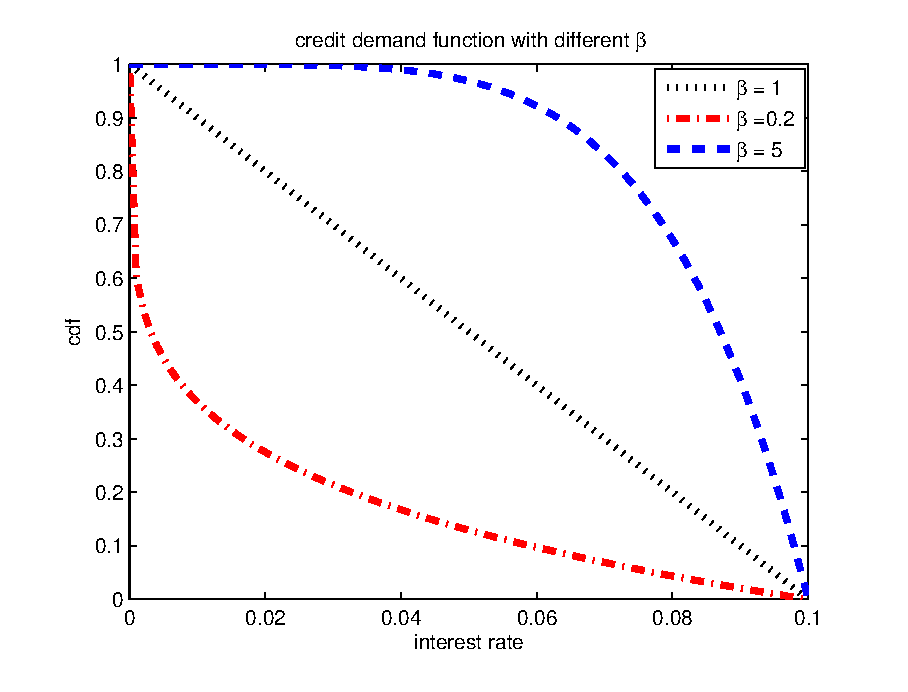
\includegraphics[width = 0.6\textwidth]{cdf.eps}
\end{center}
 \caption{The general purpose custom risk affinity firm credit demand function for various values of $\alpha$; $\nu = 0$, $\mu = 1/10$.}
\end{figure} 

\subsubsubsection{Risk Averse Borrower}\label{riskAverseBorrowerCreditDemandFunction}

This decision rule describes a firm with zero risk tolerance. The profile of the CDF is described by:

\begin{equation*}
\ell(r) = 
\hspace*{2mm}\begin{cases}
1 & \text{if\hspace*{2mm}} r \leq \xi \\ 
0 & \text{otherwise}
\end{cases},
\end{equation*}

where $r_{\text{min}}$ is a model parameter specified by the user. It is expected but not required that $\xi \ll 1$ to ensure that $\xi < \mu$ (the production markup rate) at all times. This CDF is a limiting case of \S\ref{customRiskAffinityBorrowerCreditDemandFunction} for which $\nu$ is fixed and $\alpha \longrightarrow \infty$.\newline

For convenience (to avoid numerical problems) we also impose a minimum interest rate $r_{text{min}}$ which is close to zero.  We assume for the moment that the demand function for credit can then be written in the form\newline

\subsubsection{Firm Bankruptcy Procedure}\label{firmBankruptcyProcedure}

In the standard model the number of firms does not change in time. Rather, when a firm fails it is made subject to a bankruptcy resolution process (the `firm bankruptcy handler') which will either save the firm, allowing it to continue as a going concern, or destroy the firm and regenerate it.\newline

The means through which the firm bankruptcy handler resolves the firm bankruptcy/insolvency/debt crisis is up to the implementation: firm bankruptcy handlers are objects and are model parameters in the meaning of \S\ref{modelParametersSubsection}.

\subsubsubsection{Default Condition}

Firms fail when either:

\begin{enumerate}
\item The firm fails to pay its debts or its obligations when these become due, and/or
\item The firm equity is negative: $A < L \implies E < 0$ (\S\ref{firmBalanceSheetStructure})
\end{enumerate}

Using (1) without (2) is considered to be a stronger modelling assumption.\newline

When a firm fails it is made subject to a bankruptcy handler whose purpose is to restore (or begin to restore) the financial position of the firm so that it may continue as a going concern. It is not unusual for the firm bankruptcy handler to be required to address outstanding creditor debts and the bankruptcy handler may be required to do this even if the firm has insufficient liquid or illiquid assets to finance the debt. In these circumstances the firm may be wound down and it may be the case that creditors are required to accept losses.\newline

Firm equity includes inventory evaluated at the market price, so firms can become insolvent as a result of sudden changes in the value of goods/services. The most likely trigger for the firm bankruptcy handler is cash flow insolvency in the form of failure to repay commercial loans, loan interest instalments and/or labour wages. Particular care must be taken when processing goods and labour settlements to avoid cases in which the underlying cash transaction fails as a result of otherwise negligible numerical rounding errors: such a failure could result in the firm bankruptcy handler being triggered inappropriately.\newline

The standard model provides several possible implementations of the firm bankruptcy handler. These implementations derive from a common framework as follows.

\subsubsubsection{Bankruptcy Handler Framework}\label{firmBailInProcedure}

Firm bankruptcy handlers in the standard model consist of three ordered steps:

\begin{enumerate}
\item A cash compensation algorithm object is asked to compute the maximum amount of firm liquidity, $C$, that can be used to pay existing creditor debts. In this implementation it is expected that creditor debts consist of unpaid commercial loan instalments only. Up to $C$ units of firm liquidity are paid to creditors in proportion according to the outstanding debt to each creditor.

\item Should $C$ be insufficient to repay the outstanding creditor debt, this bankruptcy resolution process resorts to a stock redistribution. A stock redistribution algorithm is triggered. If this algorithm does not fail then the bankruptcy resolution is taken to be complete and no further action is taken.

\item If stock redistribution is insufficient to compensate creditors for the outstanding firm debt, then this bankruptcy resolution algorithm liquidates the firm by erasing its existing stock instrument and cancelling all outstanding commercial loans. Firm shares are created anew with a stock price equal to the value of the total firm assets, and all shares are distributed to the firm's creditors in proportion to the debt owed to each creditor.
\end{enumerate}

This process if somewhat analogous to a commercial bank bailin procedure, and is referred to as such.\newline

The first step of this procedure (1) is to check whether the firm is financially capable of paying its outstanding debt. The cash compensation algorithm in described is required to decide how much of the existing firm liquidity can be used to pay creditors who have suffered default. The cash compensation algorithm is an object and a model parameter in the meaning of \S\ref{numericalModelParameters}. This component is illustrated in \S\ref{firmBankruptcyHandlerCashCompenstionAlgorithm}.\newline

The second step in the resolution procedure is a stock redistribution. The stock redistribution policy is an object and a model parameter in the meaning of \S\ref{numericalModelParameters}. This step is executed only if the cash compensation process (1) is insufficient to compensate firm creditors. This component is outlined in \S\ref{firmBankruptcyHandlerStockRedistributionAlgorithm}.\newline

The final step (3) is applied only if (2) still fails to compensate creditors. In this case the firm is wound down (liquidated), its stock instrument is erased, and a new firm is regenerated in its place. The initial equity of the new firm is equal to the total asset value of the liquidated firm, and shares in the regenerated firm are issued for free and exclusively to the creditors of the liquidated firm.

\paragraphsubsection{Cash Compensation}\label{firmBankruptcyHandlerCashCompenstionAlgorithm}

The cash compensation algorithm must select the maximum amount of cash $C$ that the firm is to pay to its creditors in an attempt to resolve the outstanding debt. In the standard model the cash compensation algorithm sets $C = 90\%$ of all unallocated firm deposits. If the firm has nonzero allocated cash then the compensation algorithm does not undo these allocations as this could generate additional financial problems for the firm after the bankruptcy handler has exited.\newline

The sum $C^* = \min(C, D)$ where $D$ is the total debt owed to creditors is withdrawn from the firm deposit account and distributed to creditors. Each creditor receives a proportion of $C^*$ according to the relative size of the debt owed to it. This process either satisfies the creditors (who have been repaid late) or partly satisfies all creditors. If creditors are repaid then no further action is taken and the firm bankruptcy handler terminates.\newline

Note that many goods/services are nondurable (transient), that durable goods are subject to depreciation in time, and that firm production in business cycle $\lfloor t\rfloor$ will not be realized as new capital until business cycle $\lfloor t\rfloor + 1$. For this reason auctioning firm inventory as a means of compensating creditors is not implemented (though this feature may be implemented in future).

\paragraphsubsection{Stock Redistribution}\label{firmBankruptcyHandlerStockRedistributionAlgorithm}

If firm creditors cannot be compensated out of existing firm liquidity \S\ref{firmBankruptcyHandlerCashCompenstionAlgorithm} and if no other capital is available then at this stage few options remain to the administrator. The equity of the firm is insufficient to compensate its creditors and if the firm is liquidated then all shares owned by stockholders will become worthless. If possible it is therefor prefereable for non-creditor stockholders to suffer partial stock losses and for the firm to not be liquidated: the alternative is for non-creditor stockholders to lose all of the value of their shares.\newline

The purpose of the stock redistribution algorithm is to redistribute firm shares from non-creditor stockholders to creditor stockholders in an effort to compensate creditors at the expense of other shareholders. This process is numerically equivalent to issuing new shares and diluting the firm share price.\newline

In the standard model the stock redistribution algorithm is a follows:

\begin{enumerate}
\item Ask the stock exchange for a complete list $S$ of firm stockholders.
\item Partition $S$ into two disjoint subsets $C$ and $\neg C$. $C \subset S$ is the subset of stockholders who are also firm creditors and who have suffered losses as a result of default. $\neg C$ is the subset of firm stockholders who are not creditors suffering default.
\item Add to $C$ all creditors who have suffered losses as a result of default but who are not firm stockholders. If any such creditor is incapable of holding shares in their own right, create an intermediary whose responsibility is to hold shares on behalf of the creditor. The intermediary will gradually sell any shares it comes to own in order to raise cash for the creditor.
\item Compute the total value $V$ of all shares held by agents in $\neg C$ (evaluated at the current price per share).
\item If $V \geq D$ where $D$ is the remaining debt owed to creditors after cash compensation (\S\ref{firmBankruptcyHandlerCashCompenstionAlgorithm}) then remove, without compensation, $\alpha = (100 \cdot D / V)$ percent of all shares from all non-creditor stockholders $\neg C$. Give all these shares to creditors $C$ at no cost. Each creditor in $C$ receives shares in proportion to amount of debt owed by the firm to the creditor.
\item Otherwise (if $V < D$) then the total value of shares owned by non-creditor stockholders $\neg C$ is insufficient to compensate the firm creditors. In this eventuality the equity of the firm combined with the value of its stock market capitalization is still inadequate to resolve the default. The firm is now liquidated as per \S\ref{firmLiquidationProcess}.
\end{enumerate}

\paragraphsubsection{Liquidation}\label{firmLiquidationProcess}

If after cash compensation \S\ref{firmBankruptcyHandlerCashCompenstionAlgorithm} and stock redistribution \S\ref{firmBankruptcyHandlerStockRedistributionAlgorithm} firm creditors have still not been compensated then the firm is liquidated and a new firm is regenerated in its place. The firm liquidation process has much in common with the commercial bank bailin procedure and involves two steps: stock elimination and loans consolidation.\newline

After liquidation the stock of the bankrupted firm will have zero value. All shares issued by the firm are terminated and the firm stock instrument is erased at the exchange. Existing shareholders incur capital losses (equity shocks) as a result of this erasure. All of the liabilities of the liquidated form are terminated and a new firm is regenerated. The newly regenerated firm inherits the balance sheet of the liquidated firm, so the equity of the regenerated firm is equal to the total asset value of the bankrupt firm. New shares in the regenerated firm are issued to the creditors of the liquidated firm at no cost to its creditors. Each creditor receives a number of shares proportional to the value of the debt owed to it by the liquidated firm.\newline

The liquidation/regeneration cycle is therefor a loans-to-equities conversion. The balance sheets of the lenders are modified. The lender may thereafter be required to change its portfolio composition, triggering a reaction on the markets. Creditors are likely to suffer capital losses due to the difference in value of deleted loan assets compared to newly issued stocks.\newline

The stock price of the newly regenerated firm is $E / n$ where $E$ is the equity of the new firm (the total asset value after bakruptcy resolution of the liquidated firm) and $n$ is the number of shares to issue. In the standard model, stockholders are typically commercial banks and mutual funds. Depending on the financial power of mutual funds as compared to banks, it may be the case (unlike at time $t = 0$) that the dominant initial owners of the regenerated firm are funds.

\subsubsection{Balance Sheet}\label{firmBalanceSheetStructure}

The industrial subeconomy consists of $N > 0$ firms labelled $F_1, F_2$ ... $F_N$. Each firm has an individual balance sheet in which assets and liabilities are recorded. The balance sheet of firm $F_i$ is:

\begin{table}[h]
\centering\begin{tabular}{c | c}
Assets & Liabilities \\
\hline
$A_{i0}, A_{i1}, A_{i2}$ ... & $L_{i0}, L_{i1}, L_{i2}$ ...
\end{tabular}
\end{table}

where $A_{ij}$ is the $j$th asset of firm $i$ and $L_{ik}$ is the $k$th liability of firm $i$. Note that either column may be empty (nil assets and/or nil  liabilities). Write $A_i$ for the total asset value $\sum_{j}A_{ij}$ and $L_i$ for the total liability value $\sum_j L_{ij}$. The firm equity is written $E_i = A_i - L_i$. Each element of the balance sheet is potentially a time-dependent quantity: $A_{ij} = A_{ij}(t), L_i = L_i(t)$ and so on.\newline

Balance sheets are data structures, continuously updated depending on the actions of the firms. When firms buy input goods/services the value of the capital (if any) is recorded as an inventory asset on the balance sheet. After production, spent input goods are deducted from inventory assets and newly produced goods are added in their place. Note that production is not necessarily a constant equity process, as value is added when input goods are converted to production goods. Firm liabilities include commercial loans, which are recoded at the instant new loans are taken out by the firm.

\subsubsection{Accounting}

The assumption of the standard model is that commercial banks buy all shares in newly created firms. Banks are the initial owners of firms.\newline

At time $t = 0$ it may be helpful to give newly created firms more cash than the value of their initial stock emission. This is because the simulation is meant to appear at time $t = 0$ as though it had existed at earlier times. The creation of the firm therefor involves shareholder cash as well and (optionally) supplementary cash creation from exogenous sources.  If a firm is created at any subsequent time $t > 0$, all cash should be raised via endogenous sources (stock emissions) to avoid money creation. Banks may in due course sell their shares other stock-trading agents, meaning that mutual funds and/or other non-banking agents may eventually become the owners of firms.\newline

\begin{table}[h]
\centering\begin{minipage}{0.7\linewidth}\centering
\begin{tabular}{c | c}
Assets & Liabilities \\
\hline
$C^E_{i}$ + $C^S_{i}$ & nil. \\
\end{tabular}
\label{BeginningBS}
\caption{A firm balance sheet at time $t = 0$. $C^E_{i}$ is the initial firm cash endowment not sourced from shares. $C^S_{i}$ is the cash paid by commercial banks for the initial firm share emission. If a firm is created at time $t > 0$, $C^E_i$ should be equal to zero in order to avoid money creation.}
\end{minipage}
\end{table}

Once new firms begin production and sell their goods/services via the market, the firm balance sheet will be continuously updated. In particular since the firms produces goods in business cycle $\lfloor t\rfloor$ and sells these goods in cycle $\lfloor t\rfloor+1$, the assets side of the balance sheet will include the value of the produced good evaluated at the ask price.\newline

\begin{table}[h]
\centering\begin{minipage}{0.7\linewidth}\centering
\begin{tabular}{c | c}
Assets & Liabilities \\
\hline
$C_{i}$ & $L_{i}$ \\
$p_{i}q_{i}$ & \\
\end{tabular}
\label{BeginningBS}
\caption{A firm balance sheet at time $t > 0$. $C_i(t)$ is the size of the firm cash reserve (deposits and any other liquid holdings). $L_{i}$ is the total firm liability, which is likely to include commercial loans of various maturities and interest rates. $p_i$ is the firm ask price per unit goods to be sold (the minimum selling price) and $q_i$ is the stock of saleable goods (inventory).}
\end{minipage}
\end{table}

Any inflow and outflow of money and relative changes of the values in the balance sheet are recorded.\newline

\subsubsection{Observations and Desirable Features}\label{sectionObservationsAndDesirableFeatures}

Macroeconomic business cycles in the simulator are pronounced.  With appropriate initial conditions and configuration, heterogeneous commercial loan interest rates, firm equities, and the value of dividend streams are cyclical in time. The amplitude of these endogenous business cycles can be substantial. By default the behaviour of the simulator is that mutual fund agents invest exclusively in firm and bank stocks (Ie. funds do not invest in bonds or government gilts as an alternative to stocks, although this feature can be enabled) and commercial banks have the option to invest in stocks or commercial loans. Commercial banks do not, by default, buy stock in other commercial banks due to professional competitiveness.\newline

Commercial loans are formed via a clearing market in which aggregate demand and relative aggregate supply, not the agents themselves, govern the interest rate. No agent in the system decides the interest rate for commercial loans, but rather, the commercial loan interest rate is as a result of the sum of all agent behaviours in the model. One future aim is to use a base model with an endogenous business cycle and, by extending this base model, to investigate how the business can be affected by agent decision rules, by financial regulation, by macroeconomic structures such as Input-Output (IO) networks and by other additions and modifications. We consider it to be of key interest if we find that by extending this base model with reasonable and interesting new behaviour we discover that commercial loan interest rates are less variable and that the endogenous business cycle is suppressed. This work is ongoing at the Catholic University of Milan.\newline

Fundamentalist stock return rates are less variable than commercial loan interest rates in the model.  More diverse bank investment options (for instance, mortgages) have been in development but are still not available at the time of writing. In the interests of realism we consider it to be important that commercial loans are heterogeneous and that firms should exhibit reluctance to modify their dividend payments, as is known to be the case in real economies\footnote{Brav. et al., `Payout policy in the 21st century'}.  We consider risk and reluctance to be important to commercial bank loan activities and we intend to examine this direction. We ultimately consider it to be important that bank investment options are diversified.\newline

Although the IO network is an obvious candidate for study, we do expect that the IO network is likely to exacerbate existing endogenous business cycles and contagion events rather than stabilising these behaviours.  We note that we have a variety of different IO networks at our disposal. By default the IO network structure employed in the model is an all-to-all (namely, a complete graph) Cobb-Douglas network and, owing to its flexibility, this structure is likely to be the most stable configuration. Notwithstanding this, we now briefly consider what aspects of the IO structure we might like to investigate in future:

\begin{itemize}
\item Degree Distribution Networks (DDNs).  DDNs are IO networks for which the edge set of each vertex is randomly generated.  The number of edges connected to each vertex is drawn from a distribution.  DDNs are thought to be reasonable and realistic representations of real economies, and we do in future intend to introduce this as standard for the simulator.  The Pareto Distributed Degree Network\footnote{Acemoglu et. al., The Network Origins Of Aggregate Fluctuations} is the most interesting such structure and we intend to add this. We are of the opinion that the capabilities of the codebase are more than adequate for this feature.

\item Production Chains.  Production chain networks are special types of IO network in which a distinguished group of sectors are identified as root producers (namely, manufacturers whose outputs are fundamental to the whole economy).  All other sectors in the IO network are ultimately dependent on the production activities of the root producers. Root producers sell primitive (Ie. unrefined) products that are bought by intermediate firms, which, for the sake of simplicity, we will call wholesalers. Wholesalers in turn buy from other groups of wholesalers until the last refinement step in the chain: a distinguished group of sectors, which, for the sake of simplicity, we will call retailers. Household consumption is limited to retailer firms.  This model is currently in a proof of concept state with simplified agent decision rules.

\item We intend to introduce a non-IO type firm production function (no input goods) of the form $P$ $=$ $Z \cdot L^a$ where $Z$ is the total factor productivity, $L$ is labour employed by the firm, $a$ is a customizable fixed exponent and $P$ is production. $Z$ $=$ $Z(t)$ should be subject to a random walk or lognormal random walk or discrete Ornstein Uhlenbeck (AR1) process in $t$. This has been completed.
\end{itemize}

We also note that:

\begin{itemize}
\item The tax setup in the existing model is such that government taxation on inter-firm input goods settlements does not result in firm tax credits.  For this reason, government taxation on goods cannot quite be referred to as {\footnotesize{VAT}} in the model.  We should consider means through which we can remove tax on input goods settlements whilst preserving the tax paid on consumption goods settlements.  Although more realistic, we expect that this change will not significantly affect the model.

\item Introducing buffer-stock theory for household consumption would be of interest.

\item Financial regulation by the central bank agent in the model is currently very indirect.  The central bank agent provides repo loans (typically fixed-rate interest loans collateralised by firm stocks) and, optionally, uncollateralized cash injection loans (UCILS) depending on the lending policy of the central bank.  We note that, although they are available for use, the model does not by default contain gilts, and that gilts and government bonds are tools actively utilised by central banks to regulate economies.  Without gilts moreover the central bank acts as a slow money sink with respect to repo interest payments, because the interest received by the central bank on commercial bank repo loans does not reenter the economy.  For this reason in consultation with Southampton we think that the model should, at least temporarily, be structured in such a way that central bank profits are transferred to government and that the lender of last resort should not exist in the simulation unless the government agent is also present.  This has been done at the time of writing.

\item More attention should be given to inflation and financial regulation generally in the model.

\item The model offers an AR1 TFP process with customizable standard deviation.  We tested this feature and noted that for low AR1 TFP variance the system evolved to a stead state equilibrium, for moderate AR1 TFP variance the system generated mild firm insolvency issues resolved by stock redistributions and late debt payments, and that for higher AR1 TFP variances the system generated firm liquidations and bank bankruptcies (bailouts or bailins). 

\item Stock market capitalisation by commercial banks is too high by default in the existing model.  The capitalisation of the largest UK banks is around $16\%$ of the market but this figure is exceptionally high when compared to non-UK eurozone states and the US.  This issue is linked to commercial bank PAYE and workforce expenses (or, more precisely, the lack thereof in our model).\newline\newline Labour expenses are high for UK high street banks; in the case of {Barclays} and {Santander}, labour wages have at times accounted for roughly $50$ pence per pound of all operating expenses\footnote{\path{http://reports.barclays.com/ar12/financialstatements/consolidatedfinancialstatements/incomestatement.html}}\,\footnote{\path{http://www.santanderannualreport.com/2013/en}}.  The issue of commercial bank payroll modelling has been discussed extensively.  A proposed but as yet undecided relationship $L = L(P)$ between the target bank portfolio size $P$ and required workforce $L$ would seem to be needed to ensure that shortfalls in bank labour translate into reduced bank activities.  This modelling assumption is however (a) countercyclical in boom times and would (b) result in forced stock selling activities whenever commercial banks secure unexpectedly small workforces.  To solve this issue we intend to increase the interest rate payable on deposit accounts for household deposit holders.  The resulting interest rate payable on bank deposit account liabilities in the model should be interpreted as including the cost of premises, labour and other bank operating expenses we do not model directly.
\end{itemize}

A profitable area of study would be the relationship between central bank interest rates and commercial bank leverage.  The connection between collateralised central bank loan interest rates and economic activity is well established and important to state economies, particularly the UK economy.

\subsection{Mutual Funds}\label{sectionMutualFunds}

The primary motivations for introducing funds are: (a) to provide a vehicle to trade shares owned by households and (b) to reduce the overall stock trading activity of commercial banks. In the legacy model commercial banks were the only investors in the stock market, whereas in the standard model funds typically have at least as much financial power as banks in this respect. For reasons for convenience the legacy system involved an unrealistic market structure in which households owned shares in commercial banks and banks owned all shares in firms.\newline

In the standard model commercial bank participation in the stock market is optional (and enabled by default). Commercial banks and other firms are both owned by households, but with investment decisions delegated to funds. Households partition their savings between their deposit accounts and a mutual fund investment accounts. Each household agent invests in one and only one mutual fund and households will be able to periodically revisit their fund choice. Funds will be able to invest in bank stocks and firm stocks and they are able to lend to banks and/or government via bonds.\newline

Pension funds and insurance companies are large players in the UK financial system and these agents play significant roles in stock and bond markets. Funds are non-banking establishments that provide financial services and investment opportunities to clients. In the standard model, households are the only such clients\footnote{this restriction is not strictly necessary.} and all fund assets are owned by households. The terms `mutual fund' and `fund' are interchangeable in the parlance of the standard model. Pension funds and repo--loan issing funds are planned but not yet implemented.\newline

Funds aim to: (a) maximize returns on existing assets and (b) balance liquid assets versus illiquid assets in such a way that client withdrawal requests can always be satisfied. Client--fund interactions are characterized as `contributions' if the client intends to make a new or supplementary investment and as `withdrawals' if the client wishes to liquidate an existing investment.\newline

At this point it would be beneficial to outline the similarities and differences between (a) \code{Deposit Account} assets \S\ref{depositAccountDiscussion} and (b) \code{Investment Account} \S\ref{investmentAccountDiscussion} assets.

\subsubsection{Deposit Accounts}\label{depositAccountDiscussion}

Deposit accounts are bank (deposit holder) liabilties and client (depositor) assets. Deposit accounts are implemented as instant-access synchronous transferable balance sheet contracts with no withdrawal fees. Deposit account transactions are underwritten by the bank cash reserve if a depositor requires a cash withdrawal. A deposit account transaction can fail as a result of the depositor having a low account balance or as a result of the deposit holder having insufficient liquidity. Overdraft states are not currently allowed and interest is (optionally) payable on deposits. Depending on the bank bankruptcy resolution policy, deposit accounts may or may not be protected by financial regulations: commercial bank bailins will (in the event that the bank failure is sufficiently severe) result in deposit accounts being written down, whereas bank bailouts will not.

\subsubsubsection{Interest Rates}

Interest (whether zero or otherwise) is due on all deposit accounts once per simulation cycle at time \code{DEPOSIT\_PAYMENT} in the standard model. Deposit account interest payments are not cash transactions. It is possible for commercial banks to enter negative equity states as a result of interest payments.

\subsubsubsection{Background, and the Importance of Deposit Interest}

The original `Mark One' model \S\ref{sectionBackgroundAndMarkOne} and early iterations of the standard model \S\ref{sectionStandardModelAndIOEconomy} were subject to unrealistic stock market capitalization dynamics. In the standard model commercial bank agents do not\footnote{this restriction is actively discussed and is subject to change.} employ a workforce to deliver financial services in the same way that firm agents employ (and depend on) labour for production. Labour wages are a substantial fraction of all firm expenses\footnote{neglecting mutual fund capital gains, domestic consumption is entirely financed by labour wages.}. For this reason aggregate commercial bank profits have the potential to be far larger than aggregate firm profits and, as cumulative bank dividends reflect cumulative bank profits, the long-term fundamentalist return rate (stock dividend attractiveness) of commercial banks has the potential to be far higher than for firms. In turn this means that the expected long-term total value of bank stocks is expected to be significantly higher than firm stocks in the standard model, whereas in reality the combined market capitalizations of major UK banks is roughly $17\%$ of the market, and this figure is exceptionally high in the UK as compared to other eurozone states.\newline

In an effort to extend the legacy model to produce a simulation with (a) reasonable aggregate commercial bank stock market capitalisation, (b) increased bank operating expenses and (c) lower bank margins, we began by inspecting the deposit account code itself and noted that the following logic was responsible for the interest rate payment:

{
\begin{widepage}
\begin{lstlisting}[language=Java]
   @SuppressWarnings("unused")   // Scheduled
   private void payInterest() {
      if(!isTerminated) {
         final double
            interestToPay = getValue() * getInterestRate();
         if(interestToPay == 0.0)
            return;
         
         try {
            getDepositHolder().decreaseCashReserves(interestToPay);
         } catch (final LiquidityException e) {
            getDepositHolder().cashFlowInjection(interestToPay);
            try {
               getDepositHolder().decreaseCashReserves(interestToPay);
            } catch (final LiquidityException e1) {
               throw new IllegalStateException(e1);
            }
         }
         super.incrementValue(interestToPay);
         
         Simulation.enqueue(interestPaymentEvent);
      }
\end{lstlisting}
\end{widepage}
}

\noindent The above effectively deducts the interest payment from the deposit holder twice: the first deduction is a cash deduction from the bank cash reserve (namely, a bank asset) and the second deduction is as a result of the increase in the value of the deposit account (namely, a bank liability).  Is is not necessary to make a deduction from the bank cash reserve as the interest payment is not a cash transaction, and moreover the change in the value of the deposit account affects only the deposit holder and the depositor directly. It is also the case that no cash flow appeals need to be made by the bank.\newline

The deposit account framework has accordingly been modified. It is not the responsibility of the deposit account to select the interest rate payable on existing deposits: as it stands, it is only the responsibility of the deposit account to increase the liability of the provider at regular intervals. This means that the interest rate payable on deposit accounts is a decision to be made by the bank, and this decision rule should ideally have multiple interchangeable implementations.\newline

We are content to offer two very simple deposit account interest rate decision rules for the time being.  The first implementation is a trivial "no interest" decision rule which is equivalent to the legacy behaviour.  The second implementation is a fully customizable decision rule in which the interest rate payable on a deposit account is a function of both the simulation time $t$ and the type (eg. household, mutual fund, firm) of the deposit holder:

\begin{widepage}
\begin{lstlisting}[language=Java]
/**
  * A lightweight decision rule interface for {@link DepositAccount} interest rate selection
  * algorithms.<br><br>
  * 
  * Implementations of this interface provide financial decisions about the interest rates
  * payable on {@link DepositAccount} objects. The {@link DepositAccount} for which to decide
  * the interest rate is provided as an argument, and the chosen interest rate is applied
  * to it.<br><br>
  * 
  * See also {@link DepositAccountInterestRateDecisionAlgorithm#setInterestRate(DepositAccount)}.
  * 
  * @author phillips
  */
public interface DepositAccountInterestRateDecisionAlgorithm {
   
   /**
     * Set the interest rate for the specified {@link DepositAccount} object. The argument
     * must be non-<code>null</code>. Implementations of this interface need not make the
     * interest rate decision during this method call; the interest rate decision could be
     * made at another time in a dedicated scheduled event. The implementing class should
     * document the timing of the decision process.<br><br>
     * 
     * The {@link DepositAccount} in the argument will be modified only by adjusting its
     * interest rate. No other modifications to the {@link DepositAccount} will be made
     * by this method.
     * 
     * It is expected that this method should be called once for each {@link DepositAccount}, 
     * as required, before {@link NamedEventOrderings#DEPOSIT_PAYMENT}<code>(2)</code> in the
     * simulation cycle.
     */
   public void setInterestRate(DepositAccount account);
}
\end{lstlisting}
\end{widepage}

\noindent The above interface was considered to be the simplest possible contract for a deposit account interest rate decision algorithm.  The responsibility of the implementing class is to modify the interest rate of the argument (a deposit account).\newline

The trivial implementation of this decision rule simply returns zero for all stimuli. The alternative implementation is as follows. This implementation delegates the interest rate decision $r$ to a predetermined timeseries $r(t)$ supplied by the user:

\begin{widepage}
\begin{lstlisting}[language=Java]
package eu.crisis_economics.abm.bank.strategies;

import com.google.common.base.Preconditions;
import com.google.inject.Inject;
import com.google.inject.name.Named;

import eu.crisis_economics.abm.contracts.DepositAccount;
import eu.crisis_economics.abm.contracts.Depositor;
import eu.crisis_economics.abm.firm.Firm;
import eu.crisis_economics.abm.fund.Fund;
import eu.crisis_economics.abm.household.Household;
import eu.crisis_economics.abm.model.parameters.TimeseriesParameter;

/**
  * A simple customizable implementation of the {@link DepositAccountInterestRateDecisionAlgorithm}
  * interface.<br><br>
  * 
  * This implementation delegates the {@link DepositAccount} interest rate selection decision
  * to an instance of a {@link TimeseriesParameter}. One such {@link TimeseriesParameter} must
  * be provided for the three primary types of {@link DepositAccount} {@link Depositor}: namely,
  * {@link Household}{@code s}, {@link Firm}{@code s}, {@link Fund}{@code s}, and one further
  * {@link TimeseriesParameter} for all other types of {@link Depositor} not falling into the 
  * above categories.<br><br>
  * 
  * See also {@link CustomInterestRateDecisionAlgorithm#CustomInterestRateDecisionAlgorithm(
  * TimeseriesParameter, TimeseriesParameter, TimeseriesParameter, TimeseriesParameter)} and
  * {@link DepositAccountInterestRateDecisionAlgorithm}.
  * 
  * @author phillips
  */
public final class CustomInterestRateDecisionAlgorithm
   implements DepositAccountInterestRateDecisionAlgorithm {
   
   private TimeseriesParameter<Double>
      householdInterestRate,
      firmInterestRate,
      fundInterestRate,
      otherAgentInterestRate;
   
   /**
     * Create a {@link CustomInterestRateDecisionAlgorithm} object.<br><br>
     * 
     * See also {@link DepositAccountInterestRateDecisionAlgorithm}.
     * 
     * @param householdInterestRate <br>
     *        A {@link TimeseriesParameter} whose values define the interest rate payable
     *        on all {@link Household} {@link DepositAccount}{@code s} manipulated by this
     *        object at time <code>t</code>.
     * @param firmInterestRate <br>
     *        A {@link TimeseriesParameter} whose values define the interest rate payable
     *        on all {@link Firm} {@link DepositAccount}{@code s} manipulated by this
     *        object at time <code>t</code>.
     * @param fundInterestRate <br>
     *        A {@link TimeseriesParameter} whose values define the interest rate payable
     *        on all {@link Fund} {@link DepositAccount}{@code s} manipulated by this
     *        object at time <code>t</code>.
     * @param otherAgentInterestRate <br>
     *        A {@link TimeseriesParameter} whose values define the interest rate payable
     *        on all {@link DepositAccount} objects not held by {@link Firm}, {@link Fund} or
     *        {@link Household} {@link Depositor}{@code s} at time <code>t</code>
     */
   @Inject
   public CustomInterestRateDecisionAlgorithm(
   @Named("HOUSEHOLD_INTEREST_RATE")
      TimeseriesParameter<Double> householdInterestRate,
   @Named("FIRM_INTEREST_RATE")
      TimeseriesParameter<Double> firmInterestRate,
   @Named("FUND_INTEREST_RATE")
      TimeseriesParameter<Double> fundInterestRate,
   @Named("OTHER_AGENT_TYPE_INTEREST_RATE")
      TimeseriesParameter<Double> otherAgentInterestRate
      ) {
      this.householdInterestRate = Preconditions.checkNotNull(householdInterestRate);
      this.firmInterestRate = Preconditions.checkNotNull(firmInterestRate);
      this.fundInterestRate = Preconditions.checkNotNull(fundInterestRate);
      this.otherAgentInterestRate = Preconditions.checkNotNull(otherAgentInterestRate);
   }
   
   @Override
   public void setInterestRate(DepositAccount account) {
      final Depositor
         depositor = account.getDepositor();
      if(depositor instanceof Household)
         account.setInterestRate(householdInterestRate.get());
      else if(depositor instanceof Firm)
         account.setInterestRate(firmInterestRate.get());
      else if(depositor instanceof Fund)
         account.setInterestRate(fundInterestRate.get());
      else
         account.setInterestRate(otherAgentInterestRate.get());
   }
   
}
\end{lstlisting}
\end{widepage}

\noindent Bank deposit account liabilities in the standard model are dominated by household and mutual fund deposit holders\footnote{mutual funds make financial investments on behalf of households}. We intend to increase the deposit account interest rate as a substitute for unmodelled operating expenses (bank workforce, premises) in such a way that the increased interest paid on deposits should return to households.  For this reason we elected not to increase the interest rate payable on firm deposit accounts.  We are also mindful that the simulation is subject to a transient period: the deposit account interest payment (which does not depend on bank profit margins) should be initialised after the transient period has passed.\newline

The standard nontrivial nonadaptive bank deposit account interest rate decision rule is therefor as follows:

\begin{itemize}
\item The interest rate paid by banks on household deposit accounts is $r(t) = \frac{1}{2}r_H \cdot (\tanh[(t - t_E)/w] + 1)$, where: $r_H$ is a fixed long-term interest rate to be paid to household depositors, $t_E > 0$ is a (post-transient) timescale at which the interest rate payments should begin, and $w > 0$ is the length of the time window around $t_E$ in which to smoothly increase the interest rate from $0$ to $r_H$. We found $r_H = 0.05$ $(5\%)$, $t_E = 500$ and $w = 50$ to be convenient parameters.

\item The interest rate paid for mutual fund deposits is as the above expression with $r_M$ (a long-term fund deposit interest rate) substituted for $r_H$.  We again found $r_M = 0.05$ $(5\%)$, $t_E = 500$ and $w = 50$ to be convenient parameters.

\item The interest rate payable to firms and other types of deposit holder is zero.

\end{itemize}

\subsubsection{Investment Accounts}\label{investmentAccountDiscussion}

Investments accounts differ from deposit accounts in that withdrawals are not necessarily immediate, allowed, or without fees. The change in value of an investment account reflects the performance an underlying financial product that has been bought, and the value of an investment account can decrease if the performance of the asset was poor.\newline

In the standard model all investment accounts are currently managed by mutual funds. The value of an investment account is the value of the proportion of total mutual fund assets claimed by the account. As the value of mutual fund assets changes every simulation cycle, so does the value of all investment accounts.\newline

Concretely: if a mutual fund agent has exactly two investment account liabilities of value $\pounds 0.50$ each and the fund equity is zero, then assuming no further investment accounts are opened or closed in future, thereafter the value of each investment account is $A/2$ where $A(t)$ is the combined value of all assets owned by the fund at time $t$. Investment accounts correspond to shares in the fund, with the price per share of the fund being $A(t) / n(t)$ where $n(t)$ is the total number of fund shares in existence at time $t$. Note that $n(t)$ is arbitrary.

\subsubsection{Withdrawal Planning Problem}\label{fundWithdrawalPlanningProblem}

Many markets in the standard model are synchronous clearing markets \S\ref{markets}. Trades on synchronous markets are processed at specific times in the schedule (eg. $t$ mod $1$ $=$ \code{CLEARING\_MARKET\_MATCHING}), not continuously (`on-demand'). Funds must wait until market processing in order to liquidate existing illiquid portfolio assets, so funds are subject to forward planning problems with uncertainty about their future performance on the market.\newline

Note that funds do not know their clients' future withdrawal plans. Clients are free to request withdrawals and/or make contributions at any time in the simulation cycle. For this reason the behaviour of mutual fund agents in the standard model is as follows: 

\begin{enumerate}
\item If a client makes a new contribution to a fund (and can affort the proposed investment) then the transaction takes place immediately. This is a constant equity process for both the client (who transfers cash to the fund in exchange for an equivalent value in fund shares) and for the fund (who recieves cash from the client and increases the value of its investment account liabilities).

\item If a client requests a withdrawal, this is not processed immediately. The withdrawal is executed only after markets in which the fund is involved have been processed (in order to give the fund an opportunity to raise liquidity to satisfy the withdrawal).

\item If after the markets have been processed the fund still has insufficient liquidity to honor all client withdrawals, the available fund liquidity is rationed homogeneously among withdrawees. Concretely: if two clients request a withdrawal of $\pounds 1$ each and the fund has $\pounds 1$ in liquidity after market processing then both clients will recieve $\pounds 0.50$ (and may apply to withdraw the remainder in subsequent business cycles).
\end{enumerate}

The fund must monitor the size of its cash reserve to ensure that it does not form illiquid assets with any cash set aside to fulfill withdrawals.\newline

\subsubsection{Portfolio Planning Problem}\label{fundPortfolioDecisionProblem}

A fundamental decision the fund must make is the following: given that the intended illiquid asset portfolio size is $\pounds C \geq 0$, in what ratio should $C$ be distributed among possible instruments? Equivalently: for a set of instruments $\mathcal{I}$ $=$ $\{I\}$ with expected returns $\{\mathbb{E}[r(I)] : I \in \mathcal{I}\}$, how should a fund portfolio of size $C$ be divided among $\mathcal{I}$?\newline

Further questions must be answered:

\begin{enumerate}
 \item How should $\{\mathbb{E}[r(I)] : I \in \mathcal{I}\}$ be computed?
 \item How should $P$ be distributed given (1)? (what are the weights $w(I)$ such that the planned investment in instrument $I$ is $w(I)P$?)
\end{enumerate}

In answer to (1): for stocks the estimated return on rate is precisely the same calculation used by chartist and fundamentalist banks (as outlined in \S\ref{groupsOfAgents} and detailed in \S\ref{stockReturnForecasts}). For bank bond and government gilt investments (including extended maturity implementations of the same) the expected return rate $\mathbb{E}[r]$ is taken to be the trade-weighted mean yield-to-maturity (book yield) among all contracts formed in the most recently observed business cycle:

\begin{equation*}
 \mathbb{E}[r] = \frac{\displaystyle\sum_{1\leq i\leq\mathcal{|V|}}r_iv_i}{\displaystyle\sum_{1\leq i\leq\mathcal{|V|}}v_i},
\end{equation*}

where $\mathcal{V}$ is the set of all such contracts formed in the last business cycle, $v_i$ is the principal value of the $i$th element of $\mathcal{V}$, and $r_i$ is the yield to maturity of the $i$th element of $\mathcal{V}$. Note that this formula assumes $\mathcal{V}$ is nonempty. If $\mathcal{V}$ is empty then the same estimate is formed for the next-most-recent nonempty set of contracts $\mathcal{V}$'. For other types of investment (namely, non-loan and non-stock instruments) the user must specify the means by which $\mathbb{E}[r]$ is calculated.\newline

Write $r$ for $\mathbb{E}[r]$ for the remainder of \S\ref{fundPortfolioDecisionProblem}. The algorithm used to compute $\{w(I)\}$ given $\{r(I)\}$ (and potentially some other supplementary measurements as well as $r$) is referred to interchangeably as the `portfolio allocation strategy', the `portfolio weighting strategy' or the `investments decision rule'. The standard implementations of the portfolio allocation strategy include but are not limited to:

\begin{enumerate}
\item {\bf Fixed Distribution}\newline
Arguably the simplest allocation rule (\S\ref{fixedDistributionFundPortfolioRule}). When using this portfolio allocation rule, all instruments receive the same priority regardless of risk and regardless or actual or expected return rates.

\item {\bf Fixed Loan Weight}\newline
A simple allocation strategy in which all instruments deemed to be `outgoing loans' (eg. bank bonds) receive a fixed weight $w_L$ and all other types of instrument receive a (different) weight $w_{\neg L}$ (\S\ref{fixedLoanWeightFundPortfolioRule}).

\item {\bf Linear Adaptive}\newline
An adaptive (incremental) allocation strategy in which $w(I)$ is increased or decreased according to the expected performance of $I$ as compared to the mean performance of all other instruments. This allocation strategy can result in $w(I)$ $=$ $0$ in a finite number of business cycles
 (\S\ref{linearAdaptiveFundPortfolioRule}).
 
\item {\bf Exponential Adaptive}\newline
A modified formulation of the Linear Adaptive allocation strategy. This implementation has the property that $w(I)\longrightarrow 0$ but remains nonzero if $I$ performs poorly over a prolonged period. If $I$ has performed poorly for $n$ business cycles then $\approx n$ business cycles of good performance are required to restore confidence in instrument $I$ (\S\ref{exponentialAdaptiveFundPortfolioRule}).

\item {\bf Logit}\newline
An efficient closed-form non-adaptive (non-incremental) allocation strategy (\S\ref{logitFundPortfolioRule}).

\item {\bf Noise}\newline
A noisy portfolio investment decision rule for which each $w(I)$ is determined by a mean reverting random process. Funds implementing this decision rule rule are called Noise--Trader Funds or NTFs. See \S\ref{noiseFundPortfolioRule}.
\end{enumerate}

\subsubsubsection{Fixed Distribution}\label{fixedDistributionFundPortfolioRule}

Arguably the simplest implementation of a portfolio allocation strategy. For a portfolio considering $N$ possible instruments, the decision of this strategy is to assign weight $w = 1/N$ to each instrument.

\subsubsubsection{Fixed Loan Weight}\label{fixedLoanWeightFundPortfolioRule}

A minor generalization of the fixed distribution portfolio strategy \S\ref{fixedDistributionFundPortfolioRule}. For a portfolio considering $N$ instruments of which $M \leq N$ such instruments are deemed to be `outgoing loans' (eg. bank bonds, commercial loans), the decision of this strategy is to assign weight $w_L = \xi / M$ to outgoing loan instruments and $w_{\neg L} = (1 - \xi) / (N - M)$ to all other instruments\footnote{$w_{\neg L}$ is taken to be zero if $M = N$.}.

\subsubsubsection{Linear Adaptive}\label{linearAdaptiveFundPortfolioRule}

This portfolio weighting algorithm describes an investor who will in due course favour the instruments with highest returns. This portfolio weighting algorithm will gradually increase weights for instruments whose return rates are higher than the group average and will gradually decrease weights for instruments whose return rates are below the group average.\newline

Once per business cycle the behaviour of the linear adaptive portfolio weighting algorithm is as follows:

\begin{enumerate}
\item For each instrument $I$ known to the portfolio, the return rate $r(I)$ is queried and stored in memory.
\item The mean instrument return rate $\overline{r} = \displaystyle\sum_{I}r(I)$ is computed.
\item The existing portfolio weight $w(I)$ assigned to instrument $I$ is updated as follows:
\begin{equation*}
\displaystyle w(I) \mapsto \max(w(I) + \epsilon\cdot\left(r(I) - \overline{r}\right), 0)
\end{equation*}
\item Each weight $w$ is renormalized according to:
\begin{equation*}
\displaystyle w(I) \mapsto \frac{w(I)}{\alpha},
\end{equation*}
where $\alpha = \displaystyle\sum_{\mathcal{I}}w(\mathcal{I})$ is the sum of all investment weights immediately after step (3).
\end{enumerate}

The parameter $\epsilon$ is called the `adaptation rate' and is a model parameter in the meaning of \S\ref{modelParametersSubsection}. $\epsilon \geq 0$ is required in order for the algorithm to behave as expected.\newline

The fundamental motivation for the linear adaptive weighting algorithm is that return rates are expected to diminish as overall investment increases. For instance if the total investment in commercial loan instruments is high then the availability of commercial loans is high, competition for loans is low, and on average the interest rate realized on each commercial loan is low. Contrariwise if the commercial loan interest rate $r$ is high then not only does the instrument represent an attractive investment opportunity (and merits an larger fraction of the portfolio) but an increased investment in the commercial loan instrument is expected to reduce $r$. The linear adaptive portfolio weighting algorithm is therefor expected to reach a dynamic equilibrium state in which the returns on all instruments are similar. Not that in such an equilibrium it is not necessarily the case the the income/profit per unit investment in each instrument is equal: the return rate $r(I)$ is an abstract measurement which may include (eg.) risk premia.\newline

Note that it is possible for the weight $w(I)$ to drop to zero for any instrument with poor returns.\newline

The initial weight configuration (at time $t = 0$) is typically $w(I)_{t = 0} = 1/N$ where $N$ is the number of instruments known to the portfolio.

\subsubsubsection{Exponential Adaptive}\label{exponentialAdaptiveFundPortfolioRule}

In practice the linear adaptive rule \S\ref{linearAdaptiveFundPortfolioRule} is subject to a number of shortcomings:

\begin{enumerate}
\item The adaptation rate $\epsilon$ does not depend on the distribution of returns $r(I)$ and does not depend on the variance (polarization) of existing weights $w$. For a portfolio with heterogeneous return rates/instrument weights, in practice the linear adaptive rule can be subject to a dichotomy in which it is either too slow to adapt or it will systematically overreact to changes in the market. This overreaction by the portfolio can result in disruptive financial oscillations with period 2 cycles.
l\item For instruments whose weights $w(I) \ll 1$ are small the overall change in the size of the investment resulting from $w(I) \mapsto \max(w(I) + \epsilon(\cdot(r(I)$ $-$ $\overline{r}), 0)$ can be large compared to the size of the existing investment. If the system is in a steady state for which all returns $r(I)$ are roughly equal and this state is achieved as a result of keeping one or more weights $w(I)$ small, then this would imply that $r(I)$ is likely to be sensitive to $w$ for some instruments. The linear adaptive rule tends to cause intercycle oscillations as a result of perturbing small weights excessively.

\item The linear rule tends to quickly forget about past instrument performance.

\item Portfolio weights can drop to zero rapidly if one instrument is especially attractive.
\end{enumerate}

None of these shortcomings are necessarily very poor and the linear adaptive scheme may be suitable for some applications. However a more recent portfolio weighting scheme is the exponential adaptive weighting. The exponential weight algorithm is as follows:

\begin{enumerate}
\item For each instrument $I$ known to the portfolio, the return rate $r(I)$ is queried and stored in memory.
\item The mean instrument return rate $\overline{r} = \displaystyle\sum_{I}r(I)$ is computed.
\item The existing portfolio weight $w(I)$ assigned to instrument $I$ is updated as follows:
\begin{equation*}
\displaystyle w(I) \mapsto \min(\max(w(I) \cdot (1 + || \epsilon\cdot\left(r(I) - \overline{r}\right) ||_{.99}), \xi), 1-\xi),
\end{equation*}
where $|| x ||_y$ is shorthand for $\max(\min(x, |y|), -|y|)$ and $1 \geq \xi \geq 0$ is a parameter. 
\item Each weight $w$ is renormalized according to:
\begin{equation*}
\displaystyle w(I) \mapsto \frac{w(I)}{\alpha},
\end{equation*}
where $\alpha = \displaystyle\sum_{\mathcal{I}}w(\mathcal{I})$ is the sum of all investment weights immediately after step (3).
\end{enumerate}

As for the linear rule \S\ref{linearAdaptiveFundPortfolioRule} the parameter $\epsilon$ is called the `adaptation rate' and is a model parameter \S\ref{modelParametersSubsection}. $\epsilon \geq 0$ is required in order for the algorithm to behave as expected.\newline

$\xi > 0$ is desirable but not required. The exponential adaptive rule has the property that $w(I)$ cannot drop to zero (other than artificially as a result of finite precision arithmetic) if its initial value $w(I)_{t = 0}$ is nonzero. For a portfolio with two instruments $I_1, I_2$ whose return rates $r_1 < r_2$ are fixed, the response of the exponential ruke is to reduce $w(I_1)$ by a factor of $\approx 1 + \frac{1}{2}\epsilon(r_1 - r_2) < 1$ (neglecting renormalization) once per simulation cycle. If after $N$ business cycles have elapsed the values $r_1$ and $r_2$ are swapped then for $\xi = 0$ it will take a further $2N$ business cycles for the portfolio weights $w(I_1), w(I_2)$ to invert. If $\xi > 0$ then the number of business cycles required to invert the portfolio in this way is bounded above as $N \longrightarrow \infty$ because $w(I)$ may not be less than $\xi$.\newline

In practice the exponential rule tends to perform better than the linear rule. Instruments whose portfolio weights are small and whose existing investments are small tend to be perturbed by small amounts and likewise instruments with large existing portfolio weights tend to be perturbed by larger amounts. This has the effect of reducing financial oscillations in the system.\newline

The initial weight configuration (at time $t = 0$) is typically $w(I)_{t = 0} = 1/N$ where $N$ is the number of instruments known to the portfolio.

\subsubsubsection{Logit}\label{logitFundPortfolioRule}

The logit rule is a closed--form nonadaptive portfolio weighting rule. For instruments $I$ with returns $r(I)$ the weight $w(I)$ applied to instrument $I$ is:
\begin{equation*}
w(I) = \frac{e^{\beta r(I)}}{\displaystyle\sum_J e^{\beta r(J)}},
\end{equation*}
where $J$ runs over all instruments in the portfolio and $\beta \geq 0$ is a model parameter called the `intensity of choice'.\newline

In the limit $\beta \rightarrow 0$ we have $w(I) \rightarrow \frac{1}{N}$ where $N$ is the number of instruments known to the portfolio, and for $\beta \rightarrow \infty$ we have:
\begin{equation*}
w(I) = \begin{cases}
\hspace*{1mm}1 & \text{if\,\,}r(I) = \max_J\{r(J)\}\\
\hspace*{1mm}0 & \text{otherwise.}
\end{cases}
\end{equation*}

The numerical cost of the logit rule is deceptive. It is not atypical for a logit rule to be connected to a clearing market whose purpose is to identify interest rates $r(I)$ with specific properties by evaluating many possible $\{r(I)\}$. The cumulative cost of evaluating the above exponential expressions can be nontrivial. Particular care should be taken when choosing $\beta$ in the above expression. The return rates $r(I)$ are expected to be of the order $r \sim 10^{-1}$ so $\beta \sim 100$ would result in exponentials of the order $e^{10}$.

\subsubsubsection{Noise}\label{noiseFundPortfolioRule}

Mutual funds using the noisy portfolio weighting rule are called `noise traders' or `noise-trader funds' (NTFs). The noisy portfolio rule is a mean--reverting lognormal process in which the weight $w(I)$ applied to each instrument $I$ does not follow the profit incentive, but rather the weight fluctuates randomly.\newline

The internal randomness of the above portfolio rules \S\ref{fundPortfolioDecisionProblem} is limited. In the standard model funds tend to invest heavily in the stock markets, and for this reason the volatility of the stock markets may be low when using the above rules. It is common for $N$ non-NTF mutual funds to be complemented by $\epsilon N$ ($0 \leq \epsilon \leq 1$) NTFs in order to increase the volatility of stock prices. Note that for a simulation running with Basel II regulation/procyclical leverage enabled it is expected but not required that at least one NTF be present\footnote{The procylical leverage features converts the volatility of portfolio instruments into a regulatory upper bound on commercial bank leverage. In the absence of NTFs the volatility of the stock market must be sourced from elsewhere, for instance rational firm decision rules or noisy firm production functions.}\newline

The behaviour of the noisy portfolio rule is as follows:

\begin{enumerate}
\item For each instrument $I$ known to the portfolio, return rate $r(I)$ is queried and stored in memory.

\item The existing weights $w(I)$ are perturbed as follows:
\begin{equation*}
w(I) \mapsto \exp\left(\rho\log(w(I)) + \mathcal{N}(\sigma^2)\right),
\end{equation*}
where $\mathcal{N}(\sigma^2)$ is a Gaussian distribution with mean zero and variance $\sigma^2$. $0 \leq \rho < 1$ is a customizable model parameter.
\item Each weight $w$ is renormalized according to:
\begin{equation*}
\displaystyle w(I) \mapsto \frac{w(I)}{\alpha},
\end{equation*}
where $\alpha = \displaystyle\sum_{\mathcal{I}}w(\mathcal{I})$ is the sum of all investment weights immediately after step (2).
\end{enumerate}

The initial weight configuration (at time $t = 0$) is typically $w(I)_{t = 0} = 1/N$ where $N$ is the number of instruments known to the portfolio.

\subsubsection{Observations and Desirable Features}

The immediate issues requiring attention for the fund agent type are (a) complementary fund implementations and (b) bank bond instruments. Only one fully endogenous implementation of the fund agent type (namely, mutual funds) is provided by the standard model. Bank bonds, including bank bonds of extended maturity, are supported by the standard model however these instruments are disabled by default. The primary investment opportunity for funds is therefor the stock market.

\subsubsubsection{Pension Funds}

Pension funds share some features in common with mutual funds. Money flows to pension funds via a levy on salaries and only flows out of pension funds after a household (namely, a client) retires. Pension funds are funds whose contributions are derived from labour PAYE. The pension fund receives contributions as a result of deductions made from employee wage packets, as opposed to discretionary investments made by households using surplus cash after consumption. The pension fund is ultimately required to pay households and/or individuals from this funding stream as well as from profits made form investments.\newline

Pension funds present an interesting problem for the codebase because pension funds naturally receive money from employees and pay out to unemployable individuals when their useful labour supply is at an end, which requires the standard model to provide a concept of an employee lifecycle for which penision funds are a natural companion. This in turn is likely to require households to be subdivided into households and individuals: households are static properties whereas individuals are subject to a lifecycle in which their labour supply depands on their age and their entitlement to pension fund support begins at a fixed time in the lifecycle. Under the life cycle model households become economically active at a certain age (when they start working and receiving wages) and eventually take mandatory retirement (when they start receiving a pension).\newline

Mutual funds and pension funds differ in several key respects: firstly unlike mutual funds there is no money flow from pension funds to households before the household retires. Household contributions to pension funds are also mandatory and these contributions amount to regular cash flow during periods of employment. In contrast to mutual funds, once assigned to a pension fund, households cannot move. These differences may be economically important. Further investigation will be needed in order to determine what happens to leftover pension funds upon the death of the client.

\subsubsubsection{Repo--Issuing Funds}

Repo loans (repos) are loans supplemented with default insurance collateral. Repos are issued on the contractual understanding that, in the event of the borrower's failure or inability to repay the loan, an agreed collateral asset must be transferred from the borrower to the lender as compensation. The collateral asset need not be liquid. Typically the repo collateral must be a high quality saleable asset (with government gilts being a prime example and, to a lesser extent, stocks in consistently profitable highly regarded firms). In the standard model mutual funds do not require collateral when purchasing bank bonds and funds are treated as any other creditor in the event of commercial bank default.\newline

Some (particularly American) types of fund lend to banks on a collateral repo basis. Commercial banks borrow from funds and make guarantees about existing collateral when doing so. The standard model provides repo loans between the central bank (lender of last resort) and commercial banks by default and it is expected that this feature can be extended.

\subsubsubsection{Bond Investments By Default}

Bond investments are currently implemented as part of a broad optional market called the BCL system ('bonds gilts and commercial lonas'). There are many markets in the codebase but at present the only market that provides bank bonds is one whose purpose is to clear risk-graded commercial loans, government gilts and bank bonds simultaneously. It is planned to offer an alternative implementation in which each instrument in the BCL structure is realized as a separate dedicated clearing market. In this way it will be possible to allow mutual/pension/repo funds to be involved in bond markets without requiring other classes of agents to issue or invest in government gilts as a prerequisite. This arrangement entails compromises; in particular banks are not necessarily able to efficiently optimize portfolio positions because optimization decision are not a part of the clearing process itself: the portfolio division is a decision made in advance of market processing and not during market processing.

\subsection{Macroeconomic Households}\label{sectionMacroeconomicHouseholds}
 
Households are the root owners of the economy and are the driving force behind consumption in the standard model. Collectively, households have very strong financial power. Households exchange labour services for wages and with these wages they (a) buy goods and services from the market and (b) save money in deposits accounts and in financial investment products.\newline

The maximum amount of labour available per household is a model parameter in the meaning of \S\ref{modelParametersSubsection}. This includes the possibility that the labour supply is a quantity that changes in time or is linked to other elements of the economy, including the state of the household. By default workers (employees) inelastically supply one unit of labour at a constant nominal ask wage $w$. The household is responsible for formulating the ask price per unit labour whereas the employer (eg. firms, government) is responsible for formulating the bid price. Employee compensation is ultimately selected by the market and is required to lie between the ask and bid wages.\newline

Households are typically implemented as macro (aggregated) agents as the true number of domestic properties in the UK runs into the several tens of million. The default household type in the standard model is the \code{Macrohousehold} agent. Households are able to supply labour to multiple employers concurrently. The household labour supply is a divisible finite non-transferable non-duplicable quantity and is conserved throughout the simulation cycle. The total labour supply in the system may increase or decrease between successive business cycles as new labour becomes available or as the labour supply shrinks. The labour supply is a household asset not listed on the asset side of the household balance sheet and (can be interpreted as) an employer liability not listed on the liability side of the employer balance sheet.\newline

Households and employers are free\footnote{Regulatory minimum wage is a feature of some firm and household decision rules.} to select whatever labour ask price $w$ they please. Labour assets are currently indistinguishable except in terms of wage and contract duration: labour contracts do not have an internal notion of quality, specialization, utility or productivity. Extended labour contracts (contracts lasting for more than one business cycle) are both supported by and tested for use with the standard model however these decision rules are not currently in use by any default agent types. Enabling this feature for use with the \code{Macrofirm} and \code{Macrohousehold} types would entail slight modfications to the decision rules of both.\newline

Households are free to hold their deposits with any known commercial bank. The standard model provides facilities for transferring deposit accounts between banks if a deposit holder so wishes. In practice however this feature is underutilized because there is no dedicated decision rule assocated with a household's preferred deposit account provider. This is a potentially area of interest as a major risk factor for troubled UK commercial banks is the possibility of a liquidity crisis caused by a run on existing deposit accounts (`a run on the bank').

\subsubsection{Legacy Model and Background}\label{macroeconomicHouseholdsInTheLegacyModel}

In the legacy `Mark One' model (\S\ref{sectionBackgroundAndMarkOne}) the amount of labour supplied per household per business cycle was an indivisible integer with value 1, and accordingly in the legacy model there were as many units of labour on the market as there were households agents. Labour was an indivisible asset so at any given time households were either fully employed by a unique employer or were fully unemployed.\newline

In the legacy model households held all shares in all commercial banks and these shared empowered households to exclusively collect the entire dividend stream issued by the financial system. This is an undesirable setup as not only is this structure unreaslistic but it also results in bank shares being withdrawn from households in the event of a commercial bank bailout/bailin. In this eventuality, as households have no ability to trade shares themselves, households are unable to rebuy assets lost to them as a result of the bank bankrupty process, meaning that the system is not permanently described by its initial setup unless bankruptcy and insolvency never occurs in the financial system.\newline

\subsubsection{Decision Rules}\label{householdDecisionRules}

Decisions made by household agents include:

\begin{enumerate}
\item {\bf The Consumption Budget}\newline
Households must decide the maximum amount of cash to set aside for buying new goods/services. The total nonzero sum set aside by the household for this purpose is called the `consumption budget'. The full consumption budget is never to be exceeded, but is not necessarily fully spent. Possible implementions for this decision rule are illustrated in \S\ref{householdConsumptionBudgetDecisionRule}.
\item {\bf Consumption Preferences}\newline
Once a consumption budget is chosen the household must decide how to divide the budget among goods/services. Goods are differentiated both by the sector from which they are sourced and by their durability characteristics\footnote{goods may provide durable capital and households balance sheets include inventory assets.}. Households may be motivated by competitive prices, by buffer-stock theory, utility maximization or otherwise.
\item {\bf Investments}\newline
Households must decide how much of their deposits not spent on consumption should be invested. Money invested in mutual funds is principally illiquid until maturity.
\item {\bf Labour Wage Ask Price}\newline
Households must decide the ask price per unit labour when seeking employment. Depending on the implementation of the labour market, high wage expectations may result in reduced employment prospects.
\item {\bf Labour Pool Size}\newline
The size of the labour supply per household is a model parameter in the meaning of \S\ref{modelParametersSubsection}. The labour pool size has the potential to be influenced both by the state of the household and by the state of the economy.
\end{enumerate}

\subsubsubsection{Consumption Budget}\label{householdConsumptionBudgetDecisionRule}

The household consumption budget rule is the household decision rule governing the amount of cash households are willing to spend, in each business cycle, on goods/services. The productivity and profitability of firms depends strongly on the combined size of domestic consumption budgets, and the GDP of the simulation world is reflected by the cash value of consumption.

The standard model provides the following implementations of the household budget rule:

\begin{enumerate}
\item {\bf Consumption Propensity}\newline
A budget rule describing a power-law relationship between domestic wealth and the size of the consumption budget. This rule is outlined in \S\ref{consumptionPropensityHouseholdConsumptionBudgetDecisionRule}.
\item {\bf Fixed Consumption}\newline
A simple budget rule in which households will spend a fixed amount (without borrowing) whenever deposits suffice. This rule is discussed in \S\ref{homogeneousConsumptionHouseholdConsumptionBudgetDecisionRule}.
\item {\bf Noisy Consumption}\newline
A budget rule with bounded normally distributed noise. This rule is highlighted in \S\ref{noisyConsumptionHouseholdConsumptionBudgetDecisionRule}.
\item {\bf AR1 Consumption}\newline
A forwarding implementation of the budget decision rule in which one of the above rules is smoothed in time according to a simple memory process. This rule is illustrated in \S\ref{ar1ConsumptionHouseholdConsumptionBudgetDecisionRule}.
\end{enumerate}

\paragraphsubsection{Consumption Propensity}\label{consumptionPropensityHouseholdConsumptionBudgetDecisionRule}

The `consumption propensity' household budget rule is used by default for households in the standard model. The value $B$ of the consumption budget decision is: 

\begin{equation*}
B(\lfloor t\rfloor) = \min(C\cdot W^\alpha, d),
\end{equation*}

where $\lfloor t\rfloor$ is the index of the simulation cycle in which the budget decision is made, $C$ is a customizable parameter (the `consumption propensity') and $\alpha \geq 0$ (`the wealth exponent') is a customizable parameter and $d$ is the value of the unallocated household deposits at the time the budget decision is made.\newline

Note that $\alpha = 1$ is required in order for this decision rule to scale linearly in monetary units.

\paragraphsubsection{Fixed Consumption}\label{homogeneousConsumptionHouseholdConsumptionBudgetDecisionRule}

The homogeneous consumption budget algorithm is potentially the simplest nontrivial household budget rule. In this implementation the household will set aside a fixed sum $b$ of its deposits for consumption unless the household cannot afford $b$. The final consumption budget is:

\begin{equation*}
B = \min(b, d),
\end{equation*}

where $d$ is the value of the unallocated household deposits. The value of $b$ is customizable.

\paragraphsubsection{Noisy Consumption}\label{noisyConsumptionHouseholdConsumptionBudgetDecisionRule}

The noisy consumption budget decision rule is a simple rule for which the underlying budget decision process $B$ is driven by a normal distribution:

\begin{equation*}
B(\lfloor t\rfloor) = {}_L|\mathcal{N}(\mu, \sigma^2)|_U,
\end{equation*}

where $\lfloor t\rfloor$ is the index of the simulation cycle in which the budget decision is made, ${}_L|x|_U$ is shorthand for $\min(U, \max(L, x))$ and $\mathcal{N}(\mu, \sigma^2)$ is a normal distribution with mean $\mu$ and variance $\sigma^2$. The values of $\mu, \sigma \geq 0, L$ and $U \geq L$ are customizable. Note that $U = +\infty$, $L = -\infty$ are acceptable.

\paragraphsubsection{AR1 Consumption}\label{ar1ConsumptionHouseholdConsumptionBudgetDecisionRule}

The AR1 household consumption budget rule describes a budget process with memory. The size of the household consumption budget ($B$) is exponentially smoothed with reference to a delegate consumption budget decision rule ($B^*$).\newline

This decision rule accepts any budget rule $B^*$ indicated in \S\ref{householdConsumptionBudgetDecisionRule} and yields a new decision $B$ with the following value: 

\begin{equation*}
B(\lfloor t\rfloor) = B^*(\lfloor t\rfloor) \cdot m  + B^*(\lfloor t\rfloor - 1) \cdot (1 - m),
\end{equation*}

where $\lfloor t\rfloor$ is the index of the simulation cycle in which the budget decision is made and $m$ ($0$ $\leq$ $m$ $\leq$ $1$) is a customizable parameter describing the memory of the process. In each simulation cycle $B$ is a linear combination of the decision made by $B^*$ and the last decision made by $B^*$. As $B^*$ is required to be positive, so is $B$.\newline

It is acceptable for $B^*$ to itself be an AR1 budget decision rule.

\paragraphsubsection{Desired: `Permanent Income' Budgets}

The AR1 `permanent income' budget strategy is an algorithm that selects the domestic consumption budget $B$ adaptively, as a fraction of household wealth $W$, based on past observations:

\begin{eqnarray*}
y_t &=& \psi y_{t-1} + (1-\psi) \frac{Y_t}{\overline{p}_{t-1}}, \\
\overline{p}_t &=& \frac{1}{N_S}\displaystyle\sum_{i = 1}^{N_S} p_{i, t}, \\[2ex]
b_t &=& \alpha y_t + \beta w_t, \\[2ex]
B_t &=& b_t \overline{p}_{t-1},
\end{eqnarray*}

where $y_t$ is the `real permanent income', $\overline{p}$ is the mean goods price over sectors, $Y_t$ is the nominal income at time step $t$, $N_S$ is the number of sectors, $\psi\, (0 \leq \psi \leq 1), \alpha$ and $\beta$ are customisable behavioural parameters, and $b_t$ is the `real consumption budget'.\newline

The permanent income budget algorithm reduces the volatility (variability in time) of domestic consumption, and increases the autocorrelation of budget timeseries.

\subsubsubsection{Consumption Preferences}\label{householdConsumptionPreferences}

Household (consumer) consumption preferences are the relative demands for goods/services when households go to market. Consumption preferences are a set of cash values assigned to each distinct type of goods/services households can buy. In order to decide how much of each product to buy, a household must first decide how much it is willing to spend in total: this budget decision rule is discussed in \S\ref{householdConsumptionBudgetDecisionRule}.\newline

The standard model provides several implementations of the household consumption preferences decision rule. These implementations include:

\begin{enumerate}
\item {\bf CES Aggregator}\newline
A Dixit/Stiglitz--type constant elasticity of substitution consumer utility function. Low prices represent attractive buying opportunities for consumers. This module is illustrated in \S\ref{householdCESConsumptionPreferencesDecisionRule}.
\item {\bf Homogeneous Consumption}\newline
Potentially the simplest implementation of the consumer preference decision rule. The homogeneous consumption rule exhibits no biases of any kind and assigns the same weight to all possible buying opportunities. This implementation is outlined in \S\ref{householdHomogeneousConsumptionPreferencesDecisionRule}.
\end{enumerate}

\paragraphsubsection{CES Aggregator}\label{householdCESConsumptionPreferencesDecisionRule}

The CES Aggregator rule is a Dixit/Stiglitz--type constant elasticity of substitution consumer utility function with no product quality assessment and no memory. If the market provides $N$ differentiated classes of goods/services with prices $p_1$, $p_2$ ... (per unit) then the value $D_i \geq 0$ a household intends to spend on product $i$ ($1$ $\leq$ $i$ $\leq$ $N$) is:

\begin{equation*}
D_i = \frac{p_i}{\displaystyle\sum_{i = 1}^N p_i} B,
\end{equation*}

where $B \geq 0$ is the total value of the household consumption budget (\S\ref{householdHomogeneousConsumptionPreferencesDecisionRule}) and $\rho$ ($0$ $\leq$ $\rho$ $\leq$ $1$) is a customizable model parameter.\newline

In the limit $\rho\longrightarrow 0$ this decision rule is equivalent to homogeneous consumption (\S\ref{householdHomogeneousConsumptionPreferencesDecisionRule}) and in the limit $\rho \longrightarrow \infty$ this rule is equivalent to an extreme price--competitive model in which the product with the lowest price receives the entire budget.\newline

Note that the cash sum $D_j$ must be converted into a quantity $q_j$ of goods/services when ordered from the market, namely $q_j = D_j / p_j$.

\paragraphsubsection{Homogeneous Consumption}\label{householdHomogeneousConsumptionPreferencesDecisionRule}

The homogeneous consumption preference rule is the extreme limit $\rho\longrightarrow 0$ of the CES Aggregator/Dixit--Stiglitz consumption preference rule \S\ref{householdCESConsumptionPreferencesDecisionRule}. This implementation is potentially the simplest possible realization of the household consumption preference rule.\newline

For $N$ differentiated goods/services, the cash sum $D_i \geq 0$ a household intends to spend on product type $i$ ($1$ $\leq$ $i$ $\leq$ $N$) is:

\begin{equation*}
D_i = B / N,
\end{equation*}

where $B \geq 0$ is the total value of the household consumption budget (\S\ref{householdHomogeneousConsumptionPreferencesDecisionRule}).

\subsubsubsection{Restricted Consumption}\label{restrictedConsumption}

In some cases it is useful to restrict household consumption to a subset of firms. When studying the macroeconomy the structure of the Input-Output network  is important, and for nontrivial networks it may be the case that the macroeconomy is subdivided into root producer firms (who may require large amounts of labour but relatively few input goods for production), intermediate/supply-chain firms who buy inputs from root producers and/or other intermediate firms (and who may require large quantities of input goods and relatively little labour) and retailer firms who sell directory to consumer households. In many economies there is a legal expectation that producers, distributors and retailers should be segregated, and the standard model provides for this configuration.\newline

The standard model has a configuration option that allows the user to specify which of the existing firms a household is allowed to buy from when processing the consumption preference decision rule \S\ref{householdConsumptionPreferences}. The structure of the algorithms discussed in \S\ref{householdConsumptionPreferences} is unchanged with the exception that $N$ includes only retailer firms who may sell to households.

\subsubsubsection{Investment Accounts}\label{householdInvestmentAccountContributionRule}

Once per simulation cycle households must decide how much cash to invest in/withdraw from funds. The household investment account (held by the fund) has definite value at all times except when the fund is trading and building new illiquid assets via the market\footnote{including when stock prices are adjusted.}. Fund investment accounts are listed on the fund balance sheet as abstract liabilities: funds modify the value of all investment accounts in proportion when their total asset value changes as a result of market activities.\newline

The household investment account decision is as follows: given unallocated deposits of value $d \geq 0$ and an investment account of value $I \geq 0$, decide a flow of funds $\Delta I$ satisfying $-I \leq \Delta I \leq d$ such that the household will apply for the value of the investment account to be changed from $I$ to $I + \Delta I$. If $\Delta I < 0$ then money will be withdrawn from the fund investment account and deposited with the household bank. If $\Delta I > 0$ then cash is withdrawn from the household deposit account and transferred to the fund. Note that these restrictions ensure the household cannot enter an overdraft state as a result of a fund investment.\newline

Withdrawals $\Delta I < 0$ are (a) not guaranteed to succeed if the fund has insufficient liquidity and (b) take time to process. New contributions $\Delta I > 0$ are instantaneous (\S\ref{investmentAccountDiscussion}).\newline

The standard model provides the following implementations of the household investment account contribution rule:

\begin{enumerate}
\item {\bf Withdrawal Threshold}\newline
This decision rule will attempt to maintain a fixed investment account value $I^*$. If the instantaneous value of the fund investment account is $I < I^*$ then the household will invest a fraction of its unallocated deposits into the account in order to top it up. If the value of the fund investment account is $I > I^*$ then the household will withdraw a fraction of the excess cash ($I - I^*$). This decision rule is illustrated in \S\ref{withdrawalThresholdFundContributionRule}.

\item {\bf Zero Investment}\newline
This decision rule is perhaps the simplest possible investment account decision rule. This module describes a forgetful household that has no desire to invest additional cash in funds and never applies to withdraw existing money form the fund. This implementation is outlined in \S\ref{zeroInvestmentFundContributionRule}.
\end{enumerate}

\paragraphsubsection{Withdrawal Threshold}\label{withdrawalThresholdFundContributionRule}

This module requires the household to choose a target investment account value $V$ $\geq$ $0$. Once $V$ is selected, the steps taken by the household when formulating $\Delta I$ (\S\ref{householdInvestmentAccountContributionRule}) are as follows:

\begin{enumerate}
\item If the value $I$ of the investment account is greater than $V$ then the household will apply to withdraw $\Delta I$ $=$ $\epsilon_+ (I - V)$ units of cash from the fund, where $0$ $\leq$ $\epsilon_+$ $\leq$ $1$ is a model parameter describing the rate of withdrawal of excess investments.

\item If the value $I$ of the investment account is less than $V$ then the household will contribute $\Delta I$ $=$ $\min(\epsilon_- D, V - I)$ units of cash, where $D \geq 0$ is the value of unallocated household deposits and $0$ $\leq$ $\epsilon_-$ $\leq$ $1$ is a model parameter describing the rate of investment of unallocated deposits.
\end{enumerate}

The result of this process is that the household will attempt to maintain an investment account of value $V$ by withdrawing excess investments and by contributing a fraction of its unallocated deposits to the fund when the value of the account is low.\newline

Note that $\epsilon_- = \epsilon_+ = 1$ describes a process with no contribution/withdrawal smoothing. Investments and withdrawals in this configuration are very abrupt and can induce fund liquidity crises.

\paragraphsubsection{Zero Investment}\label{zeroInvestmentFundContributionRule}

The `zero investment' contribution rule is perhaps the simplest possible household investment account decision rule. In this implementation the household will select $\Delta I = 0$ no matter what (Ie. the household will never attempt to modify the value of the investment account).\newline

This decision rule describes a model in which all changes to the value of the household investment account (if the value of the investment account is nonzero) are as a result of profits or losses made by the fund.

\subsubsubsection{Labour Wage Ask Price}

Households must gauge the value of their labour by formulating an ask price $w$ $\geq$ $0$ per unit labour. A household is free\footnote{subject to eg. possible minimum wage constraints} to propose any level of remuneration for its labour services, however a high wage proposal $w$ is likely to reduce the household employment prospects. Depending on the implementation of the labour market and the mechanism used by the market to penalize households with high wage demands, households may need to balance their wage threshold against the likelihood of finding any work.\newline

The underlying wage decision made by the household is called the `wage ask price decision rule'. The standard model provides several possible implementations as follows:

\begin{enumerate}
\item {\bf Fixed Nominal Wage Expectation}\newline
Perhaps the simplest possible household wage ask price decision rule, this implementation causes the household agent to post a fixed nominal wage ask price $w$ not depending on time and not depending on the state of any other entity in the economy. This module is descibed briefly in \S\ref{householdFixedNominalWageExpectationAlgorithm}.
\item {\bf Wage Confidence}\newline
This experimental implementation describes a households whose confidence in its ability to command high wages increases with experience. Wage ask prices steadily rise when the household is in employment, until unemployment, at which point the household loses confidence in its ability to command high wages and reduces its ask price. This implementation is outlined in \S\ref{householdWageCondfidenceWageExpectationAlgorithm}.
\end{enumerate}

\paragraphsubsection{Fixed Nominal Wage Expectation}\label{householdFixedNominalWageExpectationAlgorithm}

Potentially the simplest possible implementation of the household wage ask price decision rule, this module selects a fixed ask price $w$ per unit labour no matter what the state of the household/simulation world. $w$ is nonzero but may or may not be zero. Note that this module prohibits wage competition among households, and either restricts or entirely precludes inflation.

\paragraphsubsection{Wage Confidence}\label{householdWageCondfidenceWageExpectationAlgorithm}

This module describes a household whose confidence in its ability to command high wages increases or decreases depending on its recent employment history. The household becomes confident in its ability to command high wages if it has been fully employed in recent business cycles and the household loses confidence in its labour price if it has recently been unemployed. Note that (depending on the resolution of the simulator) one household may represent millions or thousands of individual domestic properties: a macro scale simulation provides little or no information about the distribution of individual unemployed households contained within and represented by a partly unemployed \code{Macrohousehold} agent.\newline

The steps taken by the household agent when deciding the ask price $w$ are as follows:

\begin{enumerate}
\item The labour market is asked about overall employment/unemployment in the last labour market processing session. The labour market computes the fraction of the total labour supply that was in employment, $e$ ($0$ $\leq$ $e$ $\leq$ $1$), for the most recent market session.

\item If the household is fully employed (all labour supplied by the household is currently under contract) then the household computes a wage perturbation $\Delta w = \mu w_0$ where $\mu = \epsilon (\frac{1}{e} - 1) U[0, 1]$, $0$ $\leq$ $\epsilon$ $\leq$ $1$ is a customizable model parameter, $U[0, 1]$ is a uniform distribution on the unit interval, and $w_0$ is a model parameter describing the characteristic scale on which to perturb the existing ask price.

\item If the household is not fully employed (it is not the case that all labour supplied by the household is currently under contract) then the household computes a wage perturbation $\Delta w = \epsilon e U[0, 1] w_0$ (where $\epsilon$ is as above, and $U[0, 1]$ is a uniform distribution on the unit interval).

\item The perturbations $\Delta w_t, \Delta w_{t - 1} \, ... \, \Delta w_{t - T}$ (where $\Delta w_x$ is the value of the above perturbation computed in simulation cycle $x$) are summed and averaged for a number of past cycles $T$, where $T \geq 0$ is a model parameter. The resulting smoothed wage perturbation $\Delta^*$ is applied to $w$: $w \mapsto w + \Delta^*$.
\end{enumerate}

The expression $(\frac{1}{e} - 1)$ is chosen because for a simple labour model with $L$ fixed units of labour supply and $L^* \leq L$ fixed units of labour demand (which are guaranteed to be realized, no matter what the labour price $w$) a random assignment of households to vacancies will result in a household being unemployed once every $(1 - \frac{L^*}{L})$ $=$ $1 - e$ business cycles. If a variable $x$ is perturbed by $+\alpha\delta$ whenever the household is in employment and perturbed by $-\delta$ whenever the household is not fully employed then the expected change in $x$ per business cycle is $e\alpha\delta - (1 - e)\delta$ $=$ $(\alpha e + e - 1)\delta$, which is equal to zero when $\alpha = (\frac{1}{e} - 1)$. Put differently, when using this balancing factor a biasless labour market is expected to have the property that the mean upward wage perturbation as a result of full household employment is equal to the mean downward wage perturbation as a result of unemployment.\newline

Note that the user must specify the initial wage ask price $w(t = 0)$. This experimental model can be improved by removing the `fully employed' versus `not fully employed' dichotomy and replacing this with (eg.) wage perturbation factors associated with each unit of unemployment.

\subsubsubsection{Labour Supply}

In each simulation cycle households are endowed with a supply of $L$ units of labour. $L$ is the maximum amount of new labour the household may put under contract in the business cycle in which it becomes available.\newline

$L$ is not strictly a decision rule because the household agent does not necessarily control $L$ or decide $L$ at its discretion. $L$ may be an exogenous quantity selected by the user, or a quantity that is derived from the utility of consumption. $L$ must be selected by an algorithm, and the standard model provides a number of possible implementation of this algorithm:

\begin{enumerate}
\item {\bf Fixed Labour Supply}\newline
Potentially the simplest possible implementation of the labour supply algorithm, this module provides a fixed amount of labour in each business cycle. $L$ has a fixed value in time not depending on the state of the household and not depending on the state of the simulation world. The value of $L$ is customizable by the user.
\item {\bf Model Parameter}\newline
The labour supply algorithm is an object and a model parameter in the meaning of \S\ref{modelParametersSubsection}. Any of the stock model parameters described in \S\ref{modelParametersSubsection} are acceptable.
\end{enumerate}

Note that, by manually specifying the size of the labour pool, it is possible to stimulate a depression in the economy.

\subsubsubsection{Household Bankruptcy}

Deposit account overdraft states are currently not permitted in the standard model. Households may suffer deposit account losses as a result of bank bankruptcies, but this state will not result in a negative deposit account value. Cash transactions that require more money than is available to the household are rejected. Households cannot enter a net debt state and are therefor not subject to bankruptcy resolution procedures. There is currently no domestic bailiff service in the standard model.

\subsubsection{Observations and Desirable Features}

Households are potentially a fruitful area of development and there are many possible extensions and generalizations of the existing household agent. The default agent implementation used by the standard model is called \code{Macrohousehold} and this agent is (as its name suggest) macro scale.

\subsubsubsection{Household Lifecycle and State Transition}

Individuals and properties evolve through a lifecycle. New dwellings begin at high value and slowly deprecate, requiring increasing labour and inputs to maintain. Unrenewed dwellings become uninhabitable and ultimately exit the market. Individuals have a birth/death lifecycle beginning as dependents, eventually maturing to working age, at which point their labour contribution increases and then declines. At retirement individuals require pension finance and state services. Some studies purposefully include marital/cohabitant states or more granular states when simulating this evolution process.\newline

It is of interest to add (eg.) a Markov transition design pattern in which an object evolves through a set of predetermined, described states. Each state of the agent expresses various characteristics, for instance consumption propensities and the labour supply. Given that the simulator is capable of discrete time event simulation, it would not be unduly difficult to add a Markov process for a specialized household agent.

\subsubsubsection{Household Bankruptcy}

All cash payments in the standard model are debit transactions. The standard model does not simulate credit cards. It is not possible for a household to become cash flow insolvent as it cannot realize an overdraft state. Introducing overdraft states would require household bankruptcy handlers to be created, and these bankruptcy handlers may involve bailiffs and durable goods auctions.\newline

In the standard model households do not sign extended contracts/repayment plans that would require them to make periodic instalments and consumption is not financed by loans. With mortgages and property collateral, repossession may become a necessary feature of household bankruptcy.

\subsubsubsection{Buffer--Stock Theory}

`Buffer--Stock' theory is a model of consumption by C. D. Carroll et al\footnote{The buffer-stock theory of saving: Some macroeconomic evidence, C. D. Carroll et al.}. Household decision rules are modular and it would not be difficult to install this feature as a supplementary rule.

\subsubsubsection{Product Attachment}

Experience has shown that the CES Aggregator consumption function \S\ref{householdCESConsumptionPreferencesDecisionRule} has some undesirable properties. For Multiple Firms Per Sector (MFPS) models in which several firms compete to produce otherwise undifferentiated goods, the CES consumption function describes a process in which nothing but retail price is important to households. Households are unable to differentiate identically priced goods of the same class when using CES, and households do not care from which firm such goods/services are sourced. This is not a realistic model of household consumption because it does not capture firm reputation or consumer brand loyalty. It is believed that there should be a quality measure attached to goods/services and that this quality measure should reflect the effort required to produce the good, as well as the total investment the went into its development.

\subsubsubsection{Consumption Polling}

In order to implement a polling ask price decision rule \S\ref{consumptionPollingFirmPriceDecisionRule} for firms it will be necessary to modify the household interface. The household agent must expose a method that (a) accepts a set of goods prices and (b) returns a set of intended consumption budgets for each goods class given the quoted prices.

\subsection{Government}\label{sectionGovernment}

\subsubsection{Motivation and Discussion}\label{governmentAgentMotivationAndDiscussion}

Two primary motivations for the inclusion of a government agent in the simulator are to:

\begin{enumerate}
\item include welfare/benefits (and create the possibility of a welfare state economy),
\item properly represent gilts\footnote{\textit{gilts} are a United Kingdom parlance for government bonds.} and government debt,
\item introduce regulatory restrictions such as minimum wage,
\item tax transactions and profits in the economy,
\item provide a commercial bank bailout service,
\item allow for the possibility of public sector consumption and government as a buyer of goods/services, and in due course to
\item facilitate a multi-country/multi-currently model in which households belong to a dedicated government's sphere of authority.
\end{enumerate}

Government welfare and benefits spending in Eurozone states can be significant: in 2014 the UK central and local governments spent in total $112.4$ billion Sterling on welfare, or roughly $\pounds 1$ of every $\pounds 7$ spent by government. This sum was dominated by social inclusion and protection expenses and was more than double the national defence budget. The welfare spending of the UK government was second only to healthcare and pension expenses in that order\footnote{\path{gov.uk/government/collections/public-expenditure-statistical-analyses-pesa}}\footnote{\path{budgetresponsibility.org.uk/economic-fiscal-outlook-march-2015/}}.\newline

In order to quantify the extent of government borrowing: at the end of 2013 the value of all gilts issued by the UK government to national banking institutions was around $\pounds 500$ billion in total. Approximately $\pounds 413$ billion in gilts has been issued to foreign entities. About 16\% of the value of all foreign issue gilts are owned by foreign central banks. According to the UKEA data, in Q4 2013 non-foreign gilts were mainly issued to monetary/financial institutions including the Bank of England. The next largest non-foreign consumers of government gilts are insurance companies and pension funds. In the UK the central government liability to pension funds and insurers seems is roughly 70\% of the liability to financial institutions including commercial and shadow banks.\newline

In the UK the average weekly wage (assuming employment) is slightly above minimum wage, so minimum wage regulations are likely to be important for realistic simulations of price-competitive labour markets. The simulator offers a number of simple decision rules for wages, and wrapping any of these in a forwarding decision rule with minimum wage regulation (at a level specified by government) is not unduly difficult. Choosing the minimum wage threshold may however involve political as well as economic considerations.\newline

Consumption is taxed by VAT (currently $20\%$) in the UK. All goods bought at retail are subject to VAT. Goods bought as part of the input-output process (namely, goods that are ingredients in production) are not subject to VAT. PAYE (labour wages) in the UK are subject to income tax, which is deductible from final pay (Ie. individuals typically never receive the taxable component of their income). In the simulator, a government agent may need to decide the level at which goods transactions and income are taxed.\newline

The simulator includes a framework for goods/services payments (`goods for cash') and PAYE (`labour for cash'), meaning that taxation can be implemented realistically as part of the cash transaction subsystem with reference to tax levels set by government. Again choosing the level of VAT/income tax may be a political as well as an economic decision. Some bonds and financial investments in the UK are taxable whereas other investments (eg. ISAs) are tax exempt.\newline

Commercial bank bailout is a rare and potentially very expensive bank insolvency resolution process. Following the 2007/08 episode the UK government recapitalized Lloyds Banking Group (Lloyds) and the Royal Bank of Scotland (RBS) and nationalized Northern Rock and Bradford and Bingley. The UK government provided guarantees for deposits up to $\pounds 50$k as well as special liquidity, creditor guarantee and asset protection schemes which at their peak amounted to $\pounds 1.2$ trillion in support and a cash outlay of $\pounds 133$ billion; seven years later in 2005 the UK government still provides around $\pounds 120$ billion in support.\newline

When large financially important commercial banks fail the government may decide to provide public funds to settle the debt and/or restore bank equities to acceptable levels. In exchange the government is expected to receive shares in the failing bank and/or take majority ownership and control of its affairs. If and when the commercial bank has been restored to a state that it can continue to operate effectively, the government may choose to sell its shares and relinquish control of the bank to private concerns. The standard model provides government bailin services, government share retention and some welfare austerity measures that may result from such a significant national expense.

\subsubsection{Decision Rules}

In the standard model the decisions made by the government agent include the following:

\begin{enumerate}
\item The VAT (goods/services) tax percentage,
\item The government consumption function,
\item The government (government bond) gilt debt target,
\item The income tax percentage,
\item The government cash reserve target,
\item The stock market participation (share resale) policy,
\item The total expenditure budget (labour, consumption and welfare/benefits) not including debt interest,
\item The wage bid price (per unit labour) for any public sector labour to employ, 
\item How (in what proportion) to subdivide the expenses budget between consumption, welfare/benefits and public sector wages.
\end{enumerate}

These decisions are outlined the following subsections.

\subsubsubsection{VAT (goods/services) tax}\label{vatGovernmentDecisionRule}

When agents in the codebase buy goods/services a proportion of the underlying flow of funds is forked from the transaction and transferred to the government agent, if the government agent is present. If the government agent is not present in the simulation then VAT--type taxation does not occur and `goods for cash' transactions are subject to no deductions.\newline

When a transaction of value $V \geq 0$ takes place (for the acquisition of $q$ units of durable/non-durable goods) the settlement system asks the government agent for a number $T_\text{g}$ ($0$ $\leq$ $T_g$ $\leq$ $1$) representing the tax deduction proportion. $T_\text{g}$ is selected by government is not necessarily constant between business cycles. The sum paid by the consider is $V$, the sum received by the supplier is $(1 - T_g)\cdot V$ and the sum received by government is $T_g \cdot V$. In the event that the consumer cannot afford to pay $V$ then the transaction is either rejected (and is not processed further) or is rationed in such a way that the consumer can afford a modified sum $V' \leq V$ (for $q' \leq q$ units of goods/services) based on its liquidity. The government therefor cannot fail to receive the appropriate tax sum if the transaction is processed. The tax income from the transaction is received immediately by the government agent.

\subsubsubsection{Consumption Function}\label{governmentConsumptionDecisionRule}

The consumption preferences problem faced by the government agent is, mathematically, the same as the consumption preferences problem faced by household agents (\S\ref{householdConsumptionPreferences}). The government must decide an overall consumption budget $B$ and then subdivide this budget among differentiated goods types. Any of the consumption preference rules used by households (as indicated in \S\ref{householdConsumptionPreferences}) are compatible with the government agent in principle. By default the standard model provides an inelastic government consumption rule with fixed preference weights.\newline

The government agent decides its preferences for goods/services according to a pseudo von-Neumann Leontief utility function with reference to a set of consumption weights $\{w_g\}_g$ where $g$ runs over all sectors in the economy. The weight terms $w$ are non-negative and are normalizable such that $\sum_g w_g = 1$. For a government consumption budget of size $B \geq 0$ the amount of money $B_g \geq 0$ the government intends to spend consuming goods of type $g$ is $w_g^*B$, where $w^*$ are the normalized weights.\newline

Note that it is acceptable for some weights $w$ to be zero. The government does not buy goods/services from sectors $g$ for which $w = 0$.\newline

Government interaction with the goods market can be disabled entirely by the user. In this configuration, all government money set aside for consumption is unused.

\subsubsubsection{Gilt Issuance}\label{governmentGiltDebtDecisionRule}

If the government agent sells bonds then it is required to decide the maximum amount of cash it is willing to borrow (the value of the gilt issue) in each business cycle. Government bonds and gilts are implemented as fixed term fixed rate coupon bonds.\newline

The standard model provides a simple decision rule in which the government will attempt to reach a target debt/gilt issue liability. The value of the gilt debt target is customizable and is specified by the user. At each market processing session the government requests to borrow up to $D \geq 0$ units of cash in gilts where $D = \max(G^* - G, 0)$, $G^*$ is the target debt value in gilts, and $G$ is the current government gilt debt value at the time of market.\newline

Note that it is acceptable for $G^*$ to be zero. In this case the government never borrows money and will not participate in bond markets.

\subsubsubsection{Income Tax}\label{governmentIncomeTaxLevelDecisionRule}

When employers in the codebase buy labour services a proportion of the underlying flow of funds if forked from the PAYE transaction to the government agent, if the government agent is present. if the government agent is not present in the simulation then labour wages and household income are not subject to tax: labour wages are subject to no deductions and households receive the entire employer labour wage expense as income.\newline

The government is required to select a number $T_w$ ($0$ $\leq T_w$ $\leq$ $1$) describing the proportion of the wage packet flow of funds that should be forked to government. When an employer pays labour wages of value $V \geq 0$ the settlement system first asks the government for the value of $T_w$. The employer receives $(1 - T_w) V$ units of untaxable income and the government receives a sum $T_w V$.\newline

In the event that the employer cannot pay $V$ then the transaction is cancelled and no labour is remunerated. If the transaction is processed then the government agent cannot fail to receive the sum $T_w V$ in tax. Income tax enters the government cash reserve immediately.

\subsubsubsection{Cash Reserve}\label{governmentCashReserveTarget}

The government cash reserve is a fully liquid government balance sheet asset endowed to the government agent at the time the simulation is initialized. Government consumption (if any) \S\ref{governmentConsumptionDecisionRule}, public sector remuneration (if any) \S\ref{governmentBudgetSubdivisionDecisionRule} and government bond interest payments (if any) \S\ref{governmentGiltDebtDecisionRule} are paid from the government cash reserve. The size of the initial government cash reserve is customizable and is specified by the user.

\subsubsubsection{Stock Market Participation}\label{governmentStockMarketParticipationPolicy}

The government agent may receive stock assets as compensation in lieu of cash for bankruptcy resolution and commercial bank bailout. In the absence of a stock market participation strategy the government will retain these assets permanently.\newline

The standard model provides a simple model of gradual government stock resale. If the government owns a total value $V \geq 0$ in stock (potentially distributed over many instruments/types of shares) then the government strategy is to plan to own $\alpha V$ in shares after the next stock market processing session. $\alpha$ ($0$ $\leq$ $\alpha$ $\leq$ $1$) is a model parameter and is specified by the user.\newline

In order to realize this asset value the government must respond to changes in the stock market price per share $p$. If the government owns $N$ shares with value $pN$ before stock market processing and if the revised price per share selected by the market is $p^*$ then the intended government stock exchange transaction is as follows:

\begin{enumerate}
\item If $p^* > p$ then the value of the government stock asset before share transactions is $p^*N$. This represents a capital gain of $(p^* - p)N$. The government aims to retain a stock portfolio of value $\alpha pN$, so the government agent bids to sell $(p^*N - \alpha pN) / p$ shares in order to realize this. The resulting flow of funds enters the government cash reserve.

\item If $p^* < p$ then the capital value of existing government shares has decreased as a result of price changes in the market. If $p^*N < \alpha pN$ then the government would be required to buy additional shares in order to realize the target stock portfolio value $\alpha pN$. In this case the government (a) takes no action if $\alpha > \frac{p^*}{p}$, and otherwise (b) sells $(p^*N - \alpha pN) / p$ shares. The resulting flow of funds, if any, enters the government cash reserve.
\end{enumerate}

This policy describes a simple stock market participation strategy in which (a) the government agent will never buy any new shares, and (b) the value of all shares owned by the government will decrease exponentially (at a rate $\alpha$) if the government is able to realize this after capital value changes: otherwise the government will retain all its shares and accept the underlying capital loss.\newline

Note, hypothetically, that if the stock price $p$ is never revised by the market then the value of the government stock portfolio evolves as the series $V, \alpha V, \alpha^2V ...$. When $n$ simulation cycles have elapsed the value of the portfolio is $V(1 - \alpha^{n + 1}) / (1 - \alpha)$, a quantity that is never zero. For this reason the user is asked to specify a cutoff value threshold $V^* > 0$ at which point the government will attempt to sell its entire outstanding stock portfolio without regard for further exponential decreases in value: when $V < V^*$ then the target government portfolio investment value is zero rather than $\alpha V$. If this numerical cutoff $V^* > 0$ is strictly positive then in principle the government agent is able to sell the entire stock portfolio in a finite number of business cycles. It is acceptable for the user to select $V^* = 0$.

\subsubsubsection{Expenses}\label{governmentExpensesBudgetDecisionRule}

In the same way that household agents are required to select a consumption budget $B \geq 0$ before buying goods/services (\S\ref{householdConsumptionBudgetDecisionRule}), the government agent is required to select an expenses budget $B \geq 0$ to be divided between welfare/benefits, public sector wages and consumption.\newline

In the standard model the default government expenses budget decision rule is as follows:

\begin{enumerate}
\item At the end of the business cycle the government examines its cash reserve and finds $C \geq 0$ units of unallocated cash.
\item If $C > C^*$, the target cash reserve size, then the total government expenses budget is $C - C^*$.
\item Otherwise if $C < C^*$ (the value of the cash reserve is less than the target value), then the government takes the following steps:
\begin{enumerate}
\item The combined cost $D$ of all bank bailouts in the timeframe $[t, t - T]$, where $T$ is a customizable time window and $t$ is the current simulation time, is computed.
\item The total tax revenue $R \geq 0$ from the last business cycle is computed.
\item The government expenses budget is set to $B = \max(\frac{9}{10}R - \frac{D}{T}, 0)$.
\end{enumerate}
\end{enumerate}

$T \geq 0$ is a model parameter representing the characteristic timescale over which bailout losses should be recuperated from tax revenue. If $T = 10$ years and the government immediately pays $X$ units of cash to finance a bailout, then the government will attempt to set aside $X / 10$ units of cash per year from the incoming tax stream in order to restore its cash reserve to pre-bailout levels within $10$ years. If bailout expenses are low then the government will spend the entire or nearly the entire tax revenue stream on public sector workforce, consumption and/or welfare and benefits.\newline

$C^*$ is a model parameter representing the ideal or intended size of the government cash reserve. In the standard model $C^*$ is equal to the size of the initial government cash endowment (the amount of cash with which the government is initialized at startup).\newline

Note that although it is acceptable to configure a simulation in such a way that the government has no outgoings (no public sector workforce, no requirement for capital or goods/services, no welfare expenses and no bond market participation) this configuration will result in a money sink because tax revenue collected by government has no means of re-entering the economy.\newline

Once the expenses budget $B$ is decided the government must further decide how to distribute $B$ between (a) public sector wages (\S\ref{governmentWageAskPriceDecisionRule}), (b) new goods/services (\S\ref{governmentConsumptionDecisionRule}) and (c) welfare and benefits (\S\ref{governmentBudgetSubdivisionDecisionRule}). In the standard model the government uses a fixed partition function defined by three weights $w_\ell \geq 0$, $w_g \geq 0$, $w_b \geq 0$ such that $w_s + w_b + w_g = 1$. The sum $w_\ell B$ is set aside to salary the public sector workforce, the sum $w_g B$ is set aside to finance consumption and the sum $w_b B$ is allocated to welfare and benefits (\S\ref{governmentObservationsAndDesirableFeatures}).\newline

$w_\ell, w_g$ and $w_b$ are model parameters and are customizable by the user. Note that it is acceptable for one or more of $w_\ell, w_g, w_b$ to be zero.

\subsubsubsection{Wage Ask Price and Public Sector Workforce}\label{governmentWageAskPriceDecisionRule}

Once the public sector workforce budget $B_\ell$ has been decided (\S\ref{governmentExpensesBudgetDecisionRule}) the government must further decide at what rate to salary its workforce. To this end the government must select a wage bid price $w \geq 0$ per unit public sector labour.\newline

By default the government has no priority over the labour market. The government is subject to minimum wage regulation if minimum wage regulation is in effect. Depending on the implementation of the labour market it may be the case that high ask prices $w$ per unit labour result in many candidates and low wages $w$ result in an inability to fill vacancies.

\subsubsubsection{Welfare/Benefits and Cost Breakdown}\label{governmentBudgetSubdivisionDecisionRule}

When the government agent decides the maximum welfare/benefits budget $w_b B$ it must also decide how to distribute this sum among welfare recipients in its authority. Welfare recipients (households) are required to register themselves with the government agent at instantiation (time $t$ $=$ $0$) so that the government knows to whom it must distribute these benefits. Given a list of $N$ such welfare recipients $J$ $=$ $\{j_0, j_1 \hdots j_{N-1}\}$ the government welfare distribution decision is as follows:

\begin{enumerate}
\item The maximum welfare/benefits budget per welfare recipient is computed based on a fairness criterion as $w_b B / N$ (\S\ref{governmentExpensesBudgetDecisionRule}), unless the welfare/benefits budget has size zero, or there are no welfare recipients in the authority of the government, in which case this sum is zero.

\item For each welfare recipient $j$ the government queries (a) the amount (total supply) of labour $L$ that $j$ could have provided in this business cycle and (b) the amount this labour $U \leq L$ that is unemployed/not under contract.

\item For each welfare recipient $j$ the government computes a benefits budget $w_j$ of size:
\begin{equation*}
w_j = \displaystyle\frac{Uw_b B}{LN}
\end{equation*}

\item $w_j$ is transferred to $j$ as an untaxable settlement.
\end{enumerate}

Under normal operating conditions the above welfare settlements cannot fail because the government has already budgeted for the worst case benefits scenario $\sum_{j}w_j = w_b B$.\newline

Note that in general the amount paid by the government in welfare/benefits is less than $w_b B$. The entire welfare budget will only be paid by the government agent if the economy is at $0\%$ employment.

\subsubsubsection{Background}

In one of the earliest iterations of the standard model the government welfare budget was computed according to the following recipe:

\begin{enumerate}
\item The maximum welfare/benefits budget is set to $w_b B$.
\item For each welfare recipient $j$ whose unemployment is $U_j$ and whose total labour supply is $L_j$, the sum received by $j$ in welfare/benefits is:
\begin{equation*}
w_j = \frac{U_j}{\sum_k U_k} w_b B.
\end{equation*}
\end{enumerate}

Namely, welfare recipients receive benefits according to their relative degrees of unemployment. Unforuntately it is quite possible (particularly during a VaR leverage cycle) for the total unemployment $\sum_j U_j \longrightarrow 0$. This meant that any welfare recipient with a numerically residual unemployment $U_j \approx 0$ will receive virtually the entire welfare budget when using an approach such as this.

\subsubsection{Unconventional Policy Operations}

Interventions in times of financial crisis (oft referred to as `unconventional' monetary policies) are implemented in the standard model primarily in terms of bank bankruptcy resolution policy modules. Whereas the failure of non-financial sector firms does not require any substantial action to be taken by the government agent or by the central bank agent\footnote{if present} the failure of systemically important banks may result in specific, and potentially very expensive, actions taken by the government agent. The government can use public funds (taxes) to finance unconventional policy operations.\newline

In the standard model the government is involved in the following bank bankruptcy resolution policies:

\begin{enumerate}
\item{\bf Bailout}\newline
Bailout is the process in which a government effectively pays a troubled bank $b$ in order to restore it to positive equity and ensure the continuation of its business. The government uses public funds in order to recapitalize $b$, and the government may receive shares or other forms of compensation as a result of this action. This compensation results in a short term expense to the taxpayer and may or may not result in a long term loss to the public (either in the sense that the government makes a long term profit on its transactions, or in the stronger sense that a profit is made and the public is compensated for the risk assumed and the opportunity cost of lending, or in the weaker sense that a worse or more costly scenario was averted as a result of the actions of the government).

The amount of money the government requires in order to finance a bailout is equal to the negative equity of $b$ plus an overhead to ensure the functioning of $b$ after the bailout (restoring $b$ to zero equity is not sufficient to ensure its survival). If the government does not have access to sufficient bailout funds or if the government declines to fund the bailout then another, different bankruptcy resolution technique is applied to $b$. Note that this failover resolution attempt may result in $b$ being discontinued or liquidated.

Note that a successful bailout will result in the continuation of $b$.

\item{\bf Purchase \& Assumption}\newline
Purchase and assumption ({\small P\&A}) is a bankruptcy resolution technique in which a troubled bank's operations are transferred to other, healthier peer banks. Write $b$ for the bankrupt bank and $P = \{ p_1, p_2 \hdots p_N \}$ for its peers. In the purchase and assumption scheme, the banks $p$ $\in$ $P$ take on (assume) assets and liabilities from $b$. The total value of assets assumed by each peer $p$ is proportional to its liquidity position.

When assets have been assumed by $P$, $b$'s liabilities are also distributed to peers according to the value of the assets taken over by each. Finally, these assets need to be `trued up' as their combined value is smaller than the combined liability value (as $b$ is assumed to have negative equity). This finance gap is bridged by the government agent who collects the required funds via taxes.

Note that the {\small P\&A} scheme is terminal for $b$. $b$ is wound down following the redistribution of its balance sheet assets and liabilities and its business does not continue.
\end{enumerate}

Note that it is unnecessary for the government agent to spend public funds in order to process a bank bailin as the required funds are ultimately written down by bank creditors and depositors.

\subsubsection{Observations and Desirable Features}\label{governmentObservationsAndDesirableFeatures}

The relationship between government and large public sector organisations may be modelled in more detail through the use of dedicated public sector agents than by grouping public sector bodies with existing firms (much as the Bank of England is not modelled as a high street bank). In a model for which government goods/service consumption is directed largely at or on behalf of a specific national service healthcare provider (namely the NHS in the United Kingdom) special mechanics may be necessary. The healthcare and medical service budget of the United Kingdom was $\pounds 133$bn in 2015: more than twice as large as the cost of debt servicing and second only to the cost of public sector pensions ($\pounds 149.7$bn). The precise relationship between government and pension funds is also likely to be significant to third--generation models of European economies.\newline

It should be noted that the structure of public pension arrangements in European and US economies is heterogeneous. In Germany the mandatory state pension insurance scheme (gesetzliche Rentenversicherung) is a redistributive pay as you go system in which new contributions (money paid into the fund by non-retirees) is not invested but is instead used to settle ongoing pension fund outgoings\footnote{R\"{u}diger Blaich, Aegon, \textit{Pension provision in Germany: the first and second pillars in focus}}.\newline

It would be helpful to explore the exact nature of the state regulated minimum wage decision processes, and it would also be helpful to add a mechanism to compute inflation through sampling the basket prices of representative goods. Some decisions made by the government agent, for instance the growth or otherwise of the national defence budget, the size and payment policy of the welfare budget and any central/local government intervention in the housing market and/or support for first time buyers may be motivated by political considerations as well as economic outcomes. The government's objectives are not only to serve the interests of the economy and maximize social benefits in its sphere of influence, but also to be re-elected. In may ultimately be necessary to add at least a two-party election system to the government agent and observe the economic impact of differing governance policies.

\subsection{Goods Markets}\label{goodsMarkets}

Goods markets facilitate interactions between parties who sell goods/services (producers, typically firms/establishments, and perhaps resellers, intermediaries, firesale organizers) and parties who intend to buy the same (consumers, typically households, perhaps government and/or public sector bodies, other firms) with a view to executing trades. By default the standard model is configured so that firms sell and households buy differentiated goods in exchange for cash and no other parties are involved. Government and other agent types may optionally participate in the bidding process. By default all goods contracts in the standard model are executed immediately after their inception (ie. a goods--for--cash transaction is attempted as soon as the contract is established). There is currently no notion of extended supply contracts in which producers are required to furnish consumers with agreed or prepaid goods/services at regular intervals: consumers are required to bid for goods anew as required.\newline

The goods market in the standard model is a batch processed complete bipartite graph whose disjoint node groups consist of \code{GoodsSellers} and \code{GoodsBuyers}, respectively. The \code{GoodsSeller} class represents many possible different types of agent, all of which possess inventory to sell. The \code{GoodsSeller} group is typically populated exclusively by firms. \code{GoodsBuyers}, who intend to buy new goods and services, submit bid orders to the market and specify the maximum price per unit they are willing to pay for the privilege. \code{GoodsSellers} submit ask orders to the market and specify the minimum price per unit at which they are willing to do business.\newline

The goods market matches these orders twice per simulation cycle: once in order to process the input-output (firm-to-firm) consumption/production stage, and then again to process the firm-household consumption stage. Goods not sold during the first session remain available for household consumption during the second session. The amount of trade processed during the household consumption stage typically dominates the amount of trade processed during the input-output stage by an order of magnitude or more.

\subsubsection{Goods Market Entry Point}\label{goodsMarketsEntryPoint}

When submitting orders the behaviour of the goods market is as follows:

\begin{enumerate}
\item If a party submits an ask order then the party must be an \code{GoodsSeller}, otherwise the order is rejected by the market (an exception is raised).
\item If the party submits a bid order then the party must be a \code{CashAllocating}\footnote{An agent with the ability to allocate cash to use for a specific future purpose, in this case buying goods/services.} \code{GoodsBuyer}, otherwise the order cannot be processed.
\item \code{GoodsSellers} must be able to allocate sufficient inventory for the order, otherwise the order is rejected by the market on the basis that the ask party cannot deliver the promised resources.
\item \code{GoodsBuyers} are required to allocate sufficient cash at the price specified by their bid order (the maximum price to pay per unit new goods/services). If the \code{GoodsBuyer} fails to allocate this sum but can allocate a lesser nonzero sum then the order size is reduced proportionally. If the \code{GoodsBuyer} cannot allocate any cash then the order is rejected by the market.
\end{enumerate}

The bid and ask price (price per unit goods/services) must be positive for all market participants.

\subsubsection{Background and Legacy Model}\label{goodsMarketsBackgroundAndLegacyModel}

The legacy mark one (\S\ref{sectionBackgroundAndMarkOne}) model had no input-output network. $L \geq 0$ units of labour employed at time $t$ were worth $\alpha L^\beta$ units of abstract durable capital for some numbers $\alpha$, $\beta$. This abstract durable capital was used for production and decayed exponentially with each passing simulation cycle.\newline

The legacy model was believed to be subject to numerical problems caused by floating point rounding errors in cash and goods allocation. Many markets in the standard model require participants to allocate (set aside) all resources they intend to trade at the time the order is submitted: in this case buyer cash and seller inventory. In some cases these allocated resources are ultimately represented by encapsulated floating point numbers. For this reason the size of the allocation and the quantity of tradeable resources owned by the participant may be different to the order of the unit of least machine precision. In the legacy model this discrepancy was believed to be sufficient to cause the market to fully reject an order and therefor sporadically exlude a participant, which in the case of the goods market, could lead to artificial firm bankruptcies. The current implementation of the goods market is such that order sizes are automatically scaled down in the event that a participant cannot allocate the required resources but can allocate a lesser nonzero quantity.

\subsubsection{Contract Matching}\label{goodsMarketMatching}

The labour market is processed by an \code{GoodsBuyer}-\code{GoodsSeller} matching algorithm. The matching algorithm is required to do the following:

\begin{enumerate}
\item accept sets of bipartite input nodes $F$ (\code{GoodsSellers}) and $H$ (\code{GoodsBuyers}) who have submitted ask orders $A$ and bid orders $B$ (respectively) as follows:
\begin{enumerate}
\item bid orders $B$ of the form $(h, p, d)$ where $h \in H$ is a \code{GoodsBuyer}, $p \geq 0$ is the bid price per unit goods/services to buy and $d > 0$ is the quantity required by the \code{GoodsBuyer} (the demand). Write $p = p(h)$ for the bid price specified by $h$ and $d(h)$ for the demand.
\item ask orders $A$ of the form $(f, p^*, s)$ where $f \in F$ is a \code{GoodsSeller} (eg. a firm), $p^* \geq 0$ is the ask price per unit goods/services and $s > 0$ is the saleable quantity offered by the \code{GoodsSeller}. Write $p^*(f)$ for the ask price specified by $f$ and $s(f)$ for the supply.
\end{enumerate}
Note that \code{GoodsSellers} $f \in F$ submit goods orders to the market, not orders that are required to be fulfilled by specific agents $h \in H$. Likewise \code{GoodsBuyers} $h \in H$ submit goods orders to the market, not orders that are required to be fulfilled by particular $f \in F$.
\item formulate a set $X$ of matchings $X = \{ (f, h, q, \varrho) \}$ where $f \in F$, $h \in H$, $q > 0$ such that:
\begin{enumerate}
\item $\varrho \leq p(h)$ (the \code{GoodsBuyer} pays no more than the bid price),
\item optionally: $\varrho \geq p^*(f)$ (the \code{GoodsSeller} receives no less then the ask price).
\end{enumerate}
$X$ describes a set of possible trades between \code{GoodsBuyers} and \code{GoodsSellers}. When processing $X$ it is often of greater importance that the  \code{GoodsBuyer} pays no more than the bid price than that the \code{GoodsSeller} receives no less than the ask price. This is because the buyer is very often required to set aside (allocate) cash resources at the time the order is submitted to the market. If the execution price $\varrho$ selected by the market is greater than the bid price $p(h)$ then the transaction may fail as a result of insufficient allocated buyer cash.
\item the sum of the sizes of all goods/services contracts in which any $h \in H$ is involved is less than its demand, $d(h)$:
\begin{equation*}
\displaystyle\sum_{\displaystyle x \in X : h \in x} q(x) \leq d(h)
\end{equation*}
\item the sum of the sizes of all goods/services contracts in which any $f \in F$ is involved is less than its saleable inventory, $s(f)$:
\begin{equation*}
\displaystyle\sum_{\displaystyle x \in X : f \in x} q(x) \leq s(f)
\end{equation*}
\end{enumerate}

Note that it is acceptable for a \code{GoodsSeller} (which may be modelled on the macro scale, for instance an entire sector of competing firms) to provide goods to multiple \code{GoodsSellers}. The latter two conditions in the about specification ensure that no individual unit of goods/services is sold twice during the same market processing session.\newline

Other than that the goods market is s(a) required to find a solution satisfying the above specification, and (b) is not allowed to modify the states of the market participants, the goods market may compute a solution by any means. The means through which the goods market computes a solution are to be documented be the implementation.

\subsubsection{Rationing Precondition}\label{goodsMarketRationingStep}

Most goods markets in the standard model operate on the premise that a preconditioning step designed to reduce aggregate supply and/or reduce aggregate demand should first be applied to $B$ and/or $A$. This preconditioning step is required to reduce aggregate supply among nodes $f \in F$ and/or reduce aggregate demand among nodes $h \in H$ so that the resulting total supply is equal to total demand. It is expected, but not required, that this rationing should be applied to one but not both groups.\newline

This preconditioning step is loosely referred to as `rationing'. The rationing algorithm is therefor required to accept sets of disjoint nodes $F$ and $H$ (with bid/ask orders $B$, $A$) and either exclude some nodes from the market and/or specify limits on the proportions of orders that can be fulfilled for each market participant. The goods market rationing algorithm is an object and is a model parameter in the meaning of \S\ref{modelParametersSubsection}.\newline

Concretely, the rationing algorithm is required to coerce the existing bid/ask orders $B$, $A$ to a new set of rationed orders $A^*$, $B^*$ satisfying the following constraints:

\begin{enumerate}
\item For all $x \in B$ there exists a modified order $x^* \in B^*$ of the form $\{ h, p, d \}$ such that $0 \leq d^*(x) \leq d(x)$.
\item For all $x \in A$ there exists a modified order $x^* \in A^*$ of the form $\{ f, p^*, s \}$ such that $0 \leq s^*(x) \leq s(x)$.
\item Aggregate supply and aggregate demand are equal for $B^*$ and $A^*$:
\begin{equation*}
\displaystyle\sum_{x \in B^*} d^*(x) = \displaystyle\sum_{x \in A^*} s^*(x)
\end{equation*}
\end{enumerate}

Other than that the rationing algorithm is required to find a solution $A^*, B^*$ satisfying the above constraints, the algorithm may compute a solution by any means. The means through which the rationing algorithm computes the solution is documented by the implementation.\newline

The standard model provides the following stock implementations of the goods market rationing algorithm:

\begin{enumerate}
\item {\bf Homogeneous Rationing}\newline
Perhaps the simplest biasless rationing algorithm. This algorithm reduces the total supply of or the total demand for goods, whichever is greater, through applying a fixed multiplier to the sizes of all bid orders or to the sizes of all ask orders (but not both). This algorithm is detailed in \S\ref{goodsMarketHomogeneousRationingAlgorithm}.
\item {\bf Inhomogeneous Rationing}\newline
An efficient heterogeneous rationing algorithm in which some orders are curtailed more than others in order to match supply and demand. This algorithm is illustrated in \S\ref{goodsMarketInhomogeneousRationingAlgorithm}.
\item {\bf Greed Rationing}\newline
A rationing algorithm that penalizes participants who pose the lowest bid prices or the highest ask prices. This algorithm is outlined in \S\ref{goodsMarketGreedRationingAlgorithm}.
\end{enumerate}

\subsubsubsection{Homogeneous Rationing}\label{goodsMarketHomogeneousRationingAlgorithm}

Homogeneous rationing is perhaps the simplest possible biasless rationing algorithm. This algorithm reduces aggregate goods supply or reduces aggregate goods demand (but not both) by applying a fixed multiplier to exactly one of the \code{GoodsBuyer}/\code{GoodsSeller} node groups as follows:

\begin{enumerate}
\item Compute $d = \displaystyle\sum_{h \in H}d(h)$ and $s = \displaystyle\sum_{f \in F}s(f)$.
\item If $d = s$, then stop.
\item If $d > s$ then set $\xi = s / d$ and set $X = B$. 
\item Otherwise if $d < s$ then set $\xi = d / s$ and set $X = A$.
\item For each order $x \in X$, replace $x$ with $\{ \mu, p, \xi o \}$ where $\mu$ is the participant in $x$, $p$ is the bid/ask price specified by $x$, and $o(x)$ is the size of the order ($o = s(x)$ or $o = d(x)$).
\end{enumerate}

The resulting order sets $(B, X)$ or $(X, A)$ are rationed.\newline

Note that no internal random processes are in effect and therefor this process is deterministic.\newline

Homogeneous rationing can be implemented as a simple double pass operation over $A$ and $B$. The total computational cost is therefor $O(n)$ where $n$ is the number of market participants (in particular very nearly $2n$ total arithmetic cost).

\subsubsubsection{Inhomogeneous Rationing}\label{goodsMarketInhomogeneousRationingAlgorithm}

Inhomogeneous rationing is a generalization of the homogeneous rationing algorithm \S\ref{goodsMarketHomogeneousRationingAlgorithm} with uneven rationing of order sizes. This algorithm reduces the aggregate goods supply or reduces the aggregate goods demand (but not both) by randomly reducing the sizes of a sufficient number of orders in exactly one of the \code{GoodsBuyer}/ \code{GoodsSeller} node group as follows:\newline

For $x \in A \cup B$ write $r(x, \xi)$ for the function $r(x, \xi) = \{ \mu, p, {}_0|\xi|_1o \}$ where $\mu$ is the participant in $x$, $p$ is the bid/ask price specified by $x$, $o$ is the order size ($o = d(s)$ or $o = s(x)$), and ${}_a|q|_b$ is shorthand for $\min(\max(q, a), b)$.

\begin{enumerate}
\item Compute $d = \displaystyle\sum_{h \in H}d(h)$ and $s = \displaystyle\sum_{f \in F}s(f)$.
\item If $d = s$, then stop.
\item If $d > s$ then set $X = B$, $t = s$, $a = d$. Otherwise set $X = A$, $t = d$, $a = s$. 
\item Set $\xi = t / a$.
\item For each $x \in X$ apply $x \mapsto r(x, \xi + \Omega \epsilon \cdot (1 - \xi))$ where $\epsilon \sim U[0, 1)$ is drawn from a random uniform distribution on the unit interval and $\Omega \geq 0$ is a customizable model parameter.
\item Compute $a^* = \displaystyle\sum_{x \in X} o(x)$.
\item Set $\xi = t / a ^*$.
\item For each $x \in X$ apply $x \mapsto r(x, \xi)$.
\end{enumerate}

The resulting order sets $(B, X)$ or $(X, A)$ are rationed.\newline

Note that the expression $\epsilon \sim U[0, 1)$ depends on a random number generator and therefor in general this process will require a random number seed in order to behave deterministically.\newline

The parameter $\Omega > 0$ is a model parameter in the meaning of \S\ref{modelParametersSubsection}. The setting $\Omega = 0$ is equivalent to the homogeneous rationing algorithm \S\ref{goodsMarketHomogeneousRationingAlgorithm} because steps ($6-8$) are degenerate in this use case. $\Omega \sim 1$ is likely to yield a rationing in which some market participants are more severely penalized than others, whereas $\Omega \sim 0$ is likely to generate a mildly inhomogeneous rationing.\newline

Note that this process is a three--pass algorithm with $O(n)$ complexity where $n$ is the total number of market participants.

\subsubsubsection{Greed Rationing}\label{goodsMarketGreedRationingAlgorithm}

The greed rationing algorithm was originally devised as a mechanism to regulate wages in the labour market. The aim of this rationing algorithm is to penalize nodes whose price offerings are in excess of the mean price observed when processing the market. In the context of the goods market, this means that either \code{GoodsBuyers} who bid low prices or \code{GoodsSellers} with high selling prices are most likely to be excluded from the marketplace. This algorithm is an experimental work in progress and is included for completeness only.\newline

For $x \in A \cup B$ write $r(x, \xi)$ for the function $r(x, \xi) = \{ \mu, p, {}_0|\xi|_1o \}$ where $\mu$ is the participant in $x$, $p$ is the bid/ask price specified by $x$, $o$ is the order size ($o = d(s)$ or $o = s(x)$), and ${}_a|q|_b$ is shorthand for $\min(\max(q, a), b)$.\newline

For an array of nodes $X$, write $S^+$ for a sorting algorithm whose objective is $p(x_i) \leq p(x_{i + 1})$. $S^+$ sorts $X$ ascending with respect to the order price $p(x)$. Write $S^-$ for a sorting algorithm whose objective is $p(x_i) \geq p(x_{i+1})$. $S^-$ sorts $X$ descending with respect to the order price $p(x)$.

\begin{enumerate}
\item Compute $d = \displaystyle\sum_{h \in H}d(e)$ and $s = \displaystyle\sum_{f \in F}s(f)$.
\item If $d = s$, then stop.
\item If $d > s$ then set $X = B$, $t = s$, $a = d$ and $S = S^-$. Otherwise set $X = A$, $t = d$, $a = s$ and $S = S^+$. 
\item Set $\xi = t / a$.
\item Apply $S$ to $X$ (sort $X$ with respect to its order prices). Write $X_i$ for the $i$th element ($1 \leq i \leq |X|$) of $X$ after sorting.
\item Set $p = |X|$ and $R = (1 - \xi)a$.
\item If $o(X_p) \leq R$ then map $R \mapsto R - o(x)$, set $o(x)$ to zero and go to (8). Otherwise, map $o(x) \mapsto o(x) - R$, set $R = 0$ and stop.
\item Decrement $p$. Go to (7).
\end{enumerate}

The resulting order sets $(B, X)$ or $(X, A)$ are rationed.\newline

This rationing algorithm systematically trims order sizes, starting with the least reasonable order (with lowest bid price or highest ask price) and then continues to the next least reasonable order until the rationing is complete.\newline

Note that there are no internal random processes in effect in this algorithm and therefor it is deterministic.\newline

In general the cost of sorting an array of $n$ comparable datums is $O(n\ln n)$ flops. The cost of the instruction loop in steps $(6-8)$ is $O(n)$ flops. The total cost of this rationing algorithm is therefore $O(n\ln n)$ flops.

\subsubsection{Matching}\label{goodsMarketMatchingStepAfterRationing}

After rationing has been applied to the goods market participants (\S\ref{goodsMarketRationingStep}) the nodes $H$, $F$ will satisfy:

\begin{equation*}
\displaystyle\sum_{h \in H}d(h) = \displaystyle\sum_{f \in F}s(f) = \Lambda
\end{equation*}

where $\Lambda \geq 0$ is the total combined trade (quantity of goods) required by both \code{GoodsBuyers} and \code{GoodsSellers}.\newline

In the standard model most implementations of the goods market require a rationing preconditioning step followed by contract matching. The contract matching step is required to create a set a set $X = \{ (h, f, q, p) \}$ of matchings where $h \in H$, $f \in F$, $q > 0$ such that:
\begin{enumerate}
\item $p \leq p(h)$ (the \code{GoodsBuyer} pays no more than the bid price),
\item $p \geq p^*(f)$ (the \code{GoodsSeller} receives no less then the ask price),
\item $\displaystyle\sum_{x \in X : h \in x} q(h) = d(h)$ (goods demand is satisfied for all \code{GoodsBuyers}),
\item $\displaystyle\sum_{x \in X : f \in x} q(f) = s(f)$ (goods supply is satisfied for all \code{GoodsSellers}),
\item $\displaystyle\sum_{x \in X} q(x) = \Lambda$ (trade is maximized).
\end{enumerate}

Note that condition $(5)$ is equivalent to $(3)$ and $(4)$.\newline

The matching step is an object and is a model parameter in the meaning of \S\ref{numericalModelParameters}. Other than that the contract matching step is required to identify a set $X$ satisfying the above constraints, matching algorithms may identify $X$ by any means. The means used to derive $X$ are documented by the implementation.\newline

The standard model uses a matching step called `forager'.

\subsubsubsection{Forager}\label{goodsMarketForagerMatchingStep}

The forager node matching algorithm is a simple efficient random matching process. This algorithms assumes that a rationing preconditioning step has been applied to the market participants (\S\ref{labourMarketRationingStep}) beforehand.\newline
   
This matching algorithm abstractly interprets the first (left) bipartite node group as a set of buyers and the second (right) bipartite node group as a set of sellers. The buyer node group is initially shuffled. Trades are now executed between seller/buyer pairs, starting at the top of both columns in the following table and working downwards systematically:

\begin{center}
\begin{tabular}[H]{ c | c }
shuffled buyers (intent) & sellers (intent)\\[1ex]
\hline \rule{0pt}{3ex}
(a) buy quantity $q_1$ at price $p_1$ & (i.) sell quantity $q_1'$ at price $p_1'$ \\[1.5ex]
(b) buy quantity $q_2$ at price $p_2$ & (ii.) sell quantity $q_2'$ at price $p_2'$ \\[0.5ex]
$\vdots$ & $\vdots$
\end{tabular}
\end{center}
   
The order of iteration is as follows: beginning with buyer (a) try to establish a trade with seller (i.), then by seller (ii.), and so on. Remove sellers from the system whenever a seller's supply is exhausted by this process. When the buyer demand is exhausted, remove the buyer for the system. Repeat this process with buyer (b), and so on in the list of remaining buyers. Whenever a potential trade $(\min(q, q'), p, p')$ is identified the matching algorithm makes the following assumptions:
\begin{enumerate}
\item if the buyer price is less than the seller price, $p < p'$, then the execution price is taken to be $p$ (favouring the buyer)\footnote{As observed in \S\ref{labourMarketMatching} it is often of greater importance that the buyer (the \code{Employer}) pays no more than the bid price than that the seller (the \code{Employee}) receives no less than the ask price. This is because the buyer is very often required to set aside (allocate) cash resources at the time the order is submitted to the market. If the execution price $w$ selected by the market is greater than the bid price $\omega(e)$ then the transaction may fail as a result of insufficient allocated buyer cash. Note that in general it is not possible to satisfy the matching conditions unless the bid price is exceeded or the ask price is not met for some \code{Employer}--\code{Employee} pairs.}
\item if the seller price $p'$ $<$ $p$, then negotiation between the buyer and the seller is assumed. The resulting execution price is taken to be $(p'+p)/2$ (favouring the seller).
\end{enumerate}

Note that for matching problems with homogeneous prices $p = p' = \rho$, where $\rho \geq 0$ is a constant, the execution price of all contracts is equal to $\rho$.\newline
   
The name of this algorithm is borne out of its conceptual similarity to the behaviour of hunter gatherers, who randomly encounter natural resources and accept, out of necessity, whatever resources they find.\newline

Note that the shuffling operation depends on a random number generator and therefor in general this process will require a random number seed in order to behave deterministically.\newline

In general the cost of shuffling an array of $n$ datums is $O(n)$ flops or worse. The standard model uses a single-pass in-place biasless Fisher--Yates (Knuth) shuffle. The cost of the shuffle operation is $O(n)$. The formation of $X$ can be implemented as a single-ass double-cursor iteration visiting each node no more than once, therefore the total cost of this matching is $O(n)$.

\subsubsection{Call Auction}\label{goodsMarketCallAuction}

The standard model provides an alternative contract matching algorithm that uses the rationing \S\ref{labourMarketRationingStep} step differently.  This matching algorithm is normally referred to as the `call auction'.\newline

For a set of \code{GoodsBuyer} nodes $H$ with bid orders $B$ and a set of \code{GoodsSeller} nodes $F$ with ask orders $A$ the call auction processes the goods market as follows:

\begin{enumerate}
\item Create a function $v^- : \mathbb{R} \mapsto \mathbb{R}$ as follows:
\begin{equation*}
v^-(w) = \sum_{f \in F : w(f) \leq w} s(f) 
\end{equation*}
($v^-$ is the sum of the supply volumes of all ask orders whose prices are not greater than $w$, namely the total quantity of goods in the system that can be employed at price $w$ without undercutting the ask price).
\item Create a function $v^+ : \mathbb{R} \mapsto \mathbb{R}$ as follows:
\begin{equation*}
v^+(w) = \sum_{h \in H : w(h) \geq w} d(h) 
\end{equation*}
($v^+$ is the sum of the demand volumes of all bid orders whose prices are not less than $w$, namely the total labour in the system that can be employed at price $w$ without exceeding any bid price).
\item Identify the least execution price $w \geq 0$ such that $v^-(w) \geq v^+(w)$:
\begin{equation*}
w = \inf_x \{ x : v^-(x) - v^+(x) \geq 0, x \geq 0 \}.
\end{equation*}
\item Exclude all \code{GoodsSellers} from the market whose ask prices are greater than $w$.
\item Exclude all \code{GoodsBuyers} from the market whose bid prices are less than $w$.
\item Compute $d = \displaystyle\sum_{h \in H}d(h)$ and $s = \displaystyle\sum_{f \in F}s(f)$ for all outstanding participants.
\item If $d \not= e$ then apply a rationing step (\S\ref{goodsMarketRationingStep}) to all remaining market orders (such that $d = e$ after the application of the rationing).
\item Apply a node matching step (\S\ref{goodsMarketMatchingStepAfterRationing}) to the remaining market participants (generate a set $X$ of matchings).
\end{enumerate}

Note that unlike other implementations of the labour market in the standard model, this market processing algorithm does not in general have the property that \begin{equation*}
T = \sum_{x \in X} \ell(x) = \displaystyle\min\left(\,\sum_{h \in H} d(h), \sum_{f \in F} s(f)\right),
\end{equation*}
where the right hand side is evaluated over the original orders $A$, $B$: the total trade described by the matching $X$ is in general not maximized with respect to the bid and ask volumes stated in the original orders. The total trade $T \geq 0$ executed by the call auction is expected to be significantly less than the maximum admissible demand and supply, which in turn means that many market participants are likely to be wholly excluded from the market by the final matching $X$.\newline

The goods market call auction operates in the same way as the labour market call auction (with the clear exception that the underlying tradeable resource is a quantity of goods/services and not employee labour). See \S\ref{labourMarketCallAuction} for a discussion of the call auction in the context of the labour market.

\subsubsection{Instruments}\label{goodsMarketInstruments}

In the standard model the goods market is implemented as a collection of disjoint instruments labelled by sector. These instruments process mutually differentiated goods types (the type of goods produced by the corresponding sector). The goods market is composed of several such instruments, and these instruments may in principle involve different processing algorithms.\newline

Orders are routed to the appropriate instrument according to the type of goods sold by or required by the participant. There is currently no notion of extended goods/services contacts in which a supplier (a firm) is required to furnish a consumer (a household) with goods for an extended period. All contracts decided by the market are executed immediately after their inception and participants must post orders anew every simulation cycle as required.\newline

It is not a strict requirement that goods markets should be implemented in such a way that each instrument is processed independently.

\subsubsection{Order Cancellation}\label{goodsMarketOrderCancellation}

In general the market will be unable to satisfy all orders even if the supply of goods from a particular sector exceeds the demand for goods from that sector. Unsatisfied or partly satisfied orders not resolved by the market must be cancelled in a timely fashion.\newline

In the standard model, goods market contracts are processed twice per simulation cycle in batch. The first goods market processing session is dedicated to the input-output network (typically trades between firms) and the section session is dedicated to domestic consumption (typically trades between firms and households).

Orders are processed in the first instance for the input-output step at time  \code{GOODS\underline{\hspace*{2mm}}INPUT\underline{\hspace*{2mm}}MARKET\underline{\hspace*{2mm}}MATCHING}. The consumption market is processed at time \code{GOODS\underline{\hspace*{2mm}}CONSUMPTION\underline{\hspace*{2mm}}MARKET\underline{\hspace*{2mm}}MATCHING}. Any outstanding or unfulfilled orders are cancelled immediately after the consumption market processing session at time \code{POST\underline{\hspace*{2mm}}CONSUMPTION\underline{\hspace*{2mm}}MARKET\underline{\hspace*{2mm}}MATCHING}.\newline

Order cancellation entails the removal of the order from the participant order book (if applicable), the disallocation of any allocated liquidity associated with bid orders, and the disallocation of any inventory associated with ask orders.

\subsection{Durable Goods}
\subsubsection{Discussion}

A basic assumption of input-output (IO) simulations is that firms/establishments are partitioned into $N_S > 0$ sectors. A `sector' is a collection of competing and interacting agents producing exactly one of $N_S$ differentiated goods classes. Each firm (be it a \code{Macrofirm} \S\ref{macroeconomicFirmsSubsection} implementation or otherwise) is expected to belong to at least one sector for the purposes of processing the goods market.\newline

The differentiation of goods types will be indicated by subscripts: a quantity $q$ of goods from sector $i$ ($1 \leq i \leq N_S$) is denoted $q_i$. The IO network facilitates the exchange of goods and services for cash over the markets. Physical examples of UK sectors include Construction, Wholesale and Retail Trade, Agriculture, and resource extraction businesses such as Mining. With the increase in model richness associated with customizable IO networks and sectors, it becomes necessary to differentiate the capital properties of the goods sold in each sector.\newline

CRISIS has therefore been upgraded to include customizable durability (persistence) and reusability characteristics for goods. Write $\left\{ g_i \right\}_{i = 1}^{N_S}$ $=$ $\big\{ g_1$, $g_2$, $\hdots g_{N_S} \big\}$ for the differentiated goods types sourced from each sector. The characteristics of durable goods are defined to be: (a) damage, depreciation and/or losses suffered by the good as a result of its use as an ingredient in a manufacturing process, or as a result of domestic use (the overall reusability of the good both as an ingredient in production and its longevity as a used retail product) and (b) the evolution of the good in time (its decay properties). These properties are described by two customizable model parameters: $\delta_C$ ($0 \leq \delta_C \leq 1$), the `depreciation rate', and $\delta_D$ ($0 \leq \delta_D \leq 1$), the `decay rate', respectively.\newline

We assume that $\delta_D$ and $\delta_C$ describe exponential loss processes in the quantity $q$ of owned goods. The following table illustrates the physical meanings of these parameters:\newline\newline
%
{
\hspace*{4mm}
\begin{tabularx}{\textwidth}{ll}
$\delta_C$\hspace*{5mm} & \begin{minipage}{0.78\textwidth}The decay rate associated with the depreciation of goods due to their use as ingredients in the production process (manufacturing) or as a result of their use by consumers. $\delta_C = 0.4$ means that 40\% of goods will be destroyed when used as inputs in a production process. Note that depreciation is modelled as a decrease in the quantity of goods, as opposed to the value of owned goods: a good that has been used in production lessens in value not because the market price (per unit) is changed, but because a smaller quantity of the good remains.\end{minipage}\vspace*{4mm} \\[5ex]
$\delta_D$\hspace*{5mm} & \begin{minipage}{0.78\textwidth}The decay rate associated with the natural depreciation of goods due to the passage of time.  Decay occurs whenever the simulation advances from cycle $n$ to cycle $n + 1$. $\delta_D = 0.8$ means that 80\% of goods will be destroyed when the simulation cycle advances. \end{minipage}
\end{tabularx}\vspace*{6mm}
}
%
For a quantity $q$ of goods left unused in inventory, the quantity of goods remaining in simulation cycle $n$ is $(1 - \delta_D)^{n - 1}q$. For a quantity $q$ of capital goods with no decay in time ($\delta_D = 0$), fully utilized every time production occurs, the quantity of goods remaining in simulation cycle $n$ is $(1 - \delta_C)^{n - 1}q$. For a quantity $q$ of goods decaying in time and also depreciating as a result of use in production, the quantity remaining in simulation cycle $n$ is $\left((1 - \delta_D)(1 - \delta_C)\right)^{n - 1}q$.\newline

Note that the parameters $\delta_C$ and $\delta_D$ may differ between sectors. The setting $\delta_D = 1$, $\delta_C = 1$ is equivalent to the legacy CRISIS model.\newline

The quantities $\delta_D$ and $\delta_C$ are referred to as the `goods characteristics'.

\subsubsection{Naming Conventions and Edge Cases}
%
A good is referred to as `durable' if it is not the case that $\delta_D = 1$ and $\delta_C = 1$ (it is not the case that the good exists for exactly one business cycle and it is not the case that the good can be used exactly once). A good is referred to as `non--durable' if it is the case that $\delta_C = 1$ and $\delta_D = 1$ (it is the case that the good exists for exactly one business cycle and it is the case that the good can be used, either by firms or households, only once). A good is `persistent' if $\delta_D \not= 1$ (it is not the case that the good lasts for exactly one business cycle).\newline

The extremal configurations $\delta_C \in \left\{ 0, 1 \right\}$, $\delta_D \in \left\{ 0, 1 \right\}$ describe the following edge cases:\vspace*{5mm}\newline%
%
{
\hspace*{4mm}
\begin{tabularx}{\textwidth}{ll}
$\delta_C = 1, \delta_D = 1$\hspace*{5mm} &
\begin{minipage}{0.6\textwidth}Non--durable goods. Goods produced by manufacturers exist only in the simulation cycle in which they appear. Input goods are completely destroyed by the production process and cannot be reused. Non-durable goods represent one-off/on-demand services (eg. legal and healthcare services), perishable foods, non longlife food ingredients, reagents, single-use disposable products, and potentially also early-access services.
\end{minipage} \\[15ex]
$\delta_C = 1, \delta_D = 0$\hspace*{5mm} & 
\begin{minipage}{0.6\textwidth}Durable goods that are destroyed when used as inputs (are non-reusable) and which (virtually) do not decay in time. This class of goods represents eg. longlife foodstuffs and food ingredients, certain chemical ingredients, and medicines.\end{minipage} \\[10ex]
\end{tabularx}
\hspace*{4mm}
\begin{tabularx}{\textwidth}{ll}
$\delta_C = 0, \delta_D = 1$\hspace*{5mm} & \begin{minipage}{0.6\textwidth}Strongly time-limited durable goods. Any quantity $q$ of these goods disappears after one business cycle has elapsed. In the meantime, these goods are unaffected when used as ingredients in the production process or by households. This class of goods represents eg. licensed products such as software, batteries, and perhaps some catalysts.\end{minipage} \\[12ex]
$\delta_C = 0, \delta_D = 0$\hspace*{5mm} & \begin{minipage}{0.6\textwidth}Unphysical durable goods that are both (a) absolutely unaffected by the passage of time and (b) can be reused in the production process an unlimited number of times. Catalysts and (perhaps) some hard-wearing machining tools have $\delta_D \approx 0$, $\delta_C \approx 0$, $\delta_D\delta_C \not = 0$ -- but not $\delta_D = 0$, $\delta_C = 0$.\end{minipage} \\[8ex]
\end{tabularx}\newline\newline
}
%
\subsubsection{Inventory}\label{firmInventory}

With the addition of persistent goods (goods that do not disappear at the end of each simulation cycle) it is necessary for firms and consumers to store existing goods in inventory for extended periods. Inventory is a balance sheet asset and (by default) the value of the inventory is determined by the mean ask price of goods at market.\newline

In a macroeconomic simulation with $N_G > 0$ sectors, $N_D$ ($0$ $\leq N_D$ $\leq$ $N_G$) of these sectors may produce durable goods. A firm should be able to buy goods from the market and retain these goods in a dedicated inventory structure until either: (a) the product decays to negligible levels as a result of the passage of time or (b) the goods are exhausted owing to use in the production process. Similarly, households should have the ability to store and to differentiate between types of durable goods that they buy.\newline

Inventory is a potentially powerful feature that enables:
\begin{enumerate}
\item Extended production chains involving retailers,
\item Goods resale and firesales (to firm closeout or otherwise),
\item Insolvency resolution by foreclosure,
\item Capital goods as a component of equity. In particular, firms can develop negative equities as a result of changes in the market price of goods.
\end{enumerate}

Note that \textit{quantities} (namely, amounts of an abstract resource) in the simulator are almost invariably represented by decorated integers or, more commonly, floating point numbers. For this reason the concept of allocation\footnote{sometimes, interchangeably, referred to as `reservation' or 'blocking' in the phraseology of the standard model.} applies equally to resources that are not goods eg. shares, units of labour, cash, securities, and collateral assets, among others.\newline

For this reason an inventory can be interpreted as a general purpose object whose responsibility is to (a) provide allocation and disallocation\footnote{interchangeably: `unreservation' or 'unblocking'.} services while also (b) quoting the total volume of abstract resources that it gives access to. An inventory can be interpreted as either a physical storage medium, for instance a warehouse, in the case of durable goods, or as an abstract fa\c{c}ade regulating access to a virtual medium, for instance a bank account. An inventory that is a view of liquid bank accounts (one or more deposit accounts supplemented by cash allocation and disallocation services) is typically referred to as a \code{CashLedger}.\newline

In the standard model \code{Inventories} tend to provide lightweight flow recording and measurement services. A flow measurement in this context is a signed representation of the aggregate quantity of resources that have entered or left the underlying storage medium in a given timeframe. In the standard model, this flow measurement information is tallied automatically whenever certain \code{Inventory} services are invoked (for instance, the extraction of resources).\newline

Flow data that is tallied by inventories is reset inbetween simulation cycles. This service enables various data reporting and debugging features to inspect the aggregate movement of resources into and out of storage media without having to inspect (potentially many tens of thousands of) individual transactions involving the inventory.\newline

In the standard model an \code{Inventory} structure therefor consists of (a) allocation and disallocation services, (b) an interface to an abstract storage medium (that can be manipulated by inserting or removing resources) and (c) some transaction flow recording and memory. These constituent parts are outlined in the following subsections.

\subsubsubsection{Allocation}\label{goodsAllocation}

Inventories provide allocation and disallocation services. Allocated resources are `set aside' for specific future purposes. These purposes may never be realized, in which case a disallocation exercise must in due course be performed by the agent that allocated the resource in the first place\footnote{failure to disallocate unused allocated resources is a potent source of modelling and agent behavioural bugs.}.\newline

If a resource was allocated as part of market order, then typically the disallocation exercise is processed automatically as a result of callbacks made from the market to which the order was submitted. For instance firms set aside their production (either as inputs or consumption goods), and any unsold goods are disallocated automatically when the goods market cancels unsatisfied/unprocessed orders.\newline

Structures that provide allocation and disallocation services implement the \code{Allocating} interface. These implementations may incorporate \code{Allocating} as a mixin.\newline

\code{Allocating} objects provide the following methods:

\begin{enumerate}
\item \code{getMaximumAllocatable()}\newline

Compute the maximum non--negative volume of the underlying resource that can be allocated. This method returns zero if the underlying medium is empty or if the allocation policy of the inventory will not permit additional resources to be allocated.

\item \code{getAllocated()}\newline

Compute the total quantity of the underlying resource that is currently allocated (no matter for what purpose). Note that this method returns aggregate allocations: if $x$ units of a resource were allocated for purpose $A$ and $y$ units of a resource were allocated for purpose $B$ then the total allocation is $x + y$.

\item \code{setAllocated(double positiveAmount)}\newline

Reset the total allocated quantity. The argument must be non--negative, otherwise it is silently trimmed to zero. If the value of the argument is greater than the maximum allocatable quantity (\code{getMaximumAllocatable}) then the size of the resulting allocation may be less than desired.\newline

The value returned by this method is the quantity that has been allocated as a result of the call. The allocation policy of the \code{Inventory} determines the maximum amount that can be allocated.

\item \code{setUnallocated(double positiveAmount)}\newline

When called with argument $x$, this method is behaviourally equivalent to \code{setAllocated(V - x)} where \code{V} is the quantity currently stored in the underlying medium.

\item \code{changeAllocatedBy(double volume)}\newline

Increment the allocated quantity by a signed amount. This method is behaviourally equivalent to \code{setAllocated(getAllocated() + x)}, where \code{x} is the argument (which may be negative).

\item \code{getUnallocated()}\newline

This method is behaviourally equivalent to \code{V - getAllocated()}, where \code{V} is the quantity of the resource that is currently stored in the underlying medium.

\item \code{allocateAll()}\newline

This method is behaviourally equivalent to \code{setAllocated(\\ getMaximumAllocatable())}.

\item \code{disallocateAll()}\newline

This method is behaviourally equivalent to \code{setAllocated(0)}.

\end{enumerate}

Any specializations, supplementary services and/or limitations that may apply to the above over and above those listed, and which depend on the implementing class, are to be documented by the implementation.\newline 

When new resources (eg. goods, labour) are added to an inventory, it is understood that these resources are initially in an unallocated state. If resources are withdrawn from an inventory, and as a result of this withdrawal the total quantity of resources in the inventory is less than the allocated amount, then the allocated amount is reduced to the level that can be allocated.\newline

Note that the above interface is subject to change. The following features are desired and would not be unduly difficult to implement:

\begin{enumerate}
\item {\bf Lapse conditions}\newline
Failure to disallocate resources is one of the most fruitful sources of bugs in economics agent based modelling. This issue is characterized by a sudden or gradual reduction in the availability of resources, perhaps leading to a recession, and ultimately to extremal macroeconmic and financial system behaviour.\newline

Agents very often assume that new resources are initialized in unallocated states. If unsold goods from previous business cycles remain allocated in inventory then these goods will not be posted as new market orders and therefor not sold. This incurs a financial penalty and an opportunity cost to the agent that failed to properly disallocate its inventory. Similar effects have been observed in stock markets: note that any action that reduces the number of shares in circulation reduces supply, which in turn increases price, as demand is concentrated.\newline

It is thought that inventories should provide timestamped allocation services, viz. agents should indicate for how long they intend to allocate resources. Allocations should be subject to natural expiry dates, meaning that behavioural errors and/or defects in agent strategies resulting from their failure to disallocate resources may be more limited.

\item {\bf Allocation receipts}\newline
At present all allocations within a particular inventory are aggregated, in the sense that one allocation of size $x > 0$ followed by another allocation of size $y > 0$ results in a memoryless allocation of size $x + y$ that has no recollection of the fact that it was formed of two pieces (and likewise for disallocations).\newline

For this reason if the volume of the resource stored in the inventory (which may be cash) reduces unexpectedly, then the inventory is unable to modify existing allocations pro--rata/selectively according to the purposes for which these resources were allocated. This complicates forclosure activities, and bankruptcy resolution policies, and results in race conditions in which the soonest event to claim allocated resources is most likely to receive the promised amount (at the expense of later claims). A simple solution to this issue is to label resource allocations by purpose, so that future claims against allocated resources are binned within the inventory structure. This modification would noticeably alter the above specification.
\end{enumerate}

\subsubsubsection{Storage}\label{goodsStorage}

The storage component (\S\ref{firmInventory}) of inventory is an interface that describes a set of services which add to/reduce the volume of resources stored in an abstract medium. The storage medium may be a physical location, such as a firm warehouse, or a virtual medium such as a trading floor account, or a bank account (\S\ref{firmInventory}).\newline

Objects that are entry points for storage media implement the \code{Storage} interface. This interface may be incorporated as a mixin.\newline

The \code{Storage} interface requires the following methods:

\begin{enumerate}
\item\code{getStoredQuantity()}\newline

Get the total quantity that is stored in the underlying medium.

\item\code{boolean isEmpty()}\newline

Returns true when and only when the underlying storage medium is empty.

\item\code{double pull(double positiveAmount)}\newline
   
Immediately remove a quantity, $x$, from the underlying medium. $x$:
\begin{enumerate}
\item should be non--negative, or else the state of the object is unchanged, and this method returns zero;
\item should be less than $y = $\code{getStoredQuantity} at the instant of the call. If $x$ $>$ $y$ then $x$ is silently trimmed to $y$ and this method returns a number less than or equal to $y$.
\end{enumerate}
The value returned is the quantity of the underlying resource that was removed from the store as a result of the call. Note that this may be less than $x$ (but not greater than $x$).
     
\item\code{push(final positiveAmount)}\newline
   
Immediately add a positive quantity, $x$, to the store. If the argument $x$ is negative or zero, no action is taken. Otherwise, if $x > 0$, this method cannot fail and $x$ units will be immediately added to the store.

\item\code{void pushWithDelay(double positiveAmount)}\newline

This method is behaviourally equivalent to \code{Storage.push}, supplemented by a delay period. The argument will be treated as unavailable until the beginning of the next simulation cycle, at which point it will appear in the underlying medium.\newline

Resources that have been pushed into storage and that are subject to a delay period are referred to as `pending'.

\item\code{double setStoredQuantity(double amount)}\newline
   
Reset the stored quantity to the value, $x$, of the argument. If $x$ $<$ $0$ then $x$ is silently treated as zero.\newline

This method returns the evaluation of \code{getStoredQuantity} immediately after the operation is complete.

\item\code{void flush()}\newline

Completely remove all contents (pending and otherwise) from this store.
\end{enumerate}

Note that overdraft states are not supported by the standard model in the current version. This should be understood to mean that: (a) deposit account overdrafts, (b) shorting, and (c) processing goods that do not exist are unsupported operations. This is a purposeful design choice because central bank overdraft states are not permitted in the United Kingdom. If the user provides an implementation of the \code{Storage} interface that does allow for negative enclosed volumes (including shorting activities) then the design restrictions of their implementation should be clearly documented. Note that, in this use case, the user should exercise particular care with respect to the definition of an empty medium.

\subsubsubsection{Flow Memory}\label{inventoryFlowMeasurement}

In the standard model, data recording services (recorder sources \S\ref{recorderSourcesSection}) are processed once per simulation cycle at midnight on the simulation clock. In this way all agent behavioural activities have been fully processed before recording services are active.\newline

The data recorder is often required to measure the change $\Delta x$ in a quantity $x$ over the course of one simulation cycle, and/or the value $|\Delta|(x)$, the sum of the absolute values of all signed changes made to $x$ in the most recent cycle. Note that $|\Delta|(x)$ can take any value even if $\Delta x = 0$. This was accomplished by keeping dedicated private fields inside of all observed classes.\newline

In order to observe (eg.) $\Delta x$ or $|\Delta|(x)$ for a particular measurement $x$, the data recorder would simply call a class member function (a getter function, in Java parlance) whose purpose was to expose this dedicated field. Unfortunately this policy not only polluted the codebase with opaque fields and getters dedicated to recorder source services, but it was also the case that this idiom needed to be implemented whenever a flow measurement was required. This laborious process was prone to human error.\newline

In time it was realized that many of the flow measurements required by the standard model data recorder concerned (a) changes in the value of bank accounts, and (b) changed in the quantity of goods owned by firms. Both of these structures are operated via inventory in the standard model, so a decision was taken to streamline the data recording process somewhat and to add lightweight flow measurement services to the inventory structure. The purpose of these flow measurement services is simply to tally the change in the volume of enclosed resources whenever withdrawal or insertion operations are applied to the underlying storage. This is implemented in such a way that the \code{Inventory} API does not allow the flow measurement to be computed incorrectly.\newline

Objects that provide limited flow memory services in this way implement the \code{FlowMemory} interface. This interface may be incorporated as a mixin.\newline

The \code{FlowMemory} interface declares the following methods:

\begin{enumerate}
\item\code{void recordInflow(double positiveAmount)}\newline

Record an inflow event (resources added to the underlying storage medium). If the argument is negative or zero, no action is taken and this method does nothing.
    
\item\code{void recordOutflow(double positiveAmount)}\newline

Record an outflow (resources withdrawn from the underlying storage medium). If the argument is negative or zero, no action is taken and this method does nothing.
   
\item\code{void recordFlow(double amount)}\newline

Record a signed flow event. Depending on the argument, $x$:
\begin{enumerate}
\item if $x$ $>$ $0$ then this method is equivalent to \code{recordInflow($x$)},
\item if $x$ $<$ $0$ then this method is equivalent to \code{recordOutflow($x$)},
\item otherwise no action is taken and this method does nothing
\end{enumerate}
   
\item\code{double totalInflowAtThisTime()}\newline
   
Get the total inflow of resources in this simulation cycle (the sum of the arguments of all proper calls made to \code{recordInflow()}).

\item\code{double totalOutflowAtThisTime()}\newline

Get the total outflow of resources in this simulation cycle (the sum of the arguments of all proper calls made to \code{recordOutflow()}).

\item\code{double netFlowAtThisTime()}\newline
   
This method is equivalent to \code{totalInflowAtThisTime()} - \code{totalOutflowAtThisTime()}.

\item\code{void flush()}\newline

Reset the object to its initial state. After calling this method, the total inflow and outflow (and net flow) memories known to this object are zero.
\end{enumerate}

Note that \code{flush} would ordinarily be called just after simulation data recording is complete, in order to reset memories in time for the next processing cycle.

\subsubsubsection{Naming Conventions}\label{goodsNamingConventions}

In the legacy model (\S\ref{sectionBackgroundAndMarkOne}) goods were differentiated by integer labels. These labels represented the goods' (unique) sectors of origin. Firms in the standard model are required to track their ownership of multiple differentiated goods types. This bookkeeping requirement is especially pertinent where durable goods are concerned, because firm equity may depend on capital.\newline

At any given time, a firm in an Input--Output network of size $N$ may own nonzero quantities of $N$ mutually differentiated goods. The scheme used to label these goods (the naming convention) has nontrivial performance and scaling implications. In due course it was realized that the legacy model integer naming convention affected performance in one of two undesirable ways:

\begin{enumerate}
\item either all firms have access to a memory buffer of size $N$ such that each indexed bin in this memory represents a quantity of goods owned by the firm at the present time, in which case memories of combined size $N_FN$ are required, where $N_F$ is the number of firms, and a fraction of these memories will be empty at any particular time; or

\item firms dynamically allocate memory to keep track of the quantity of goods they own. In this use case, firms are required to create a dynamic map keyed by integers. Each firm would then bisect this data structure in order to seek out appropriate records. This idiom reduces the extremal memory requirement for firms at the expense of introducing a computational complexity roughly equal to $\log(N)$, which is required in order to perform queries on the memory (as opposed to $O(1)$ query cost in the above case).
\end{enumerate}

Although both of these implementations are likely to be satisfactory for small financial simulations, it is thought that neither is likely to scale well in future. The former uses $O(n)$ memory and has $O(1)$ computational cost at runtime. The latter has tight memory and $O(\log(N))$ computational cost (per firm, on average) at runtime.\newline

For this reason goods/services and sectors in the standard model are no longer indexed contiguously by integers. Both of these quantities are instead keyed by strings. These strings, and the factory that is responsible for producing them, are objects and are model parameters in the meaning of \S\ref{modelParametersSubsection}. It is possible to assign truthful names (eg.) `agriculture', `quarrying', `construction', `legal services' to sectors in the standard model. These names can be drawn from categorized Input--Output tables (such as those published by the United Kingdom Office of National Statistics).\newline

If the user does not specify a naming policy then simulation sector names are automatically generated according to a suffix pattern, for instance \code{SECTOR0}, \code{SECTOR1}, \code{SECTOR2} and so on.\footnote{a customizable univariate format string.}\newline

With this labelling convention, firms and agents that own multiple differentiated goods types tend to keep track of these quantities via hash tables keyed by sector names. These structures are referred to as \code{Repositories}.

\subsubsubsection{Repositories}\label{Respositories}

Firms in Input--Output networks (\S\ref{ioNetworks}) use multiple differentiated goods types as production inputs. In the standard model there are as many differentiated goods types as there are production sectors, and it is not atypical a simulation to support $50$ or more sectors.\newline

Each type of good has its own durability characteristics, so firms may need to process capital goods with a multitude of heterogeneous depreciation rates. Similarly, any households that derive utility from durable consumption goods may need to retain heterogeneous quantities of these resources from each sector.\newline

For this reason firm agents (and to a lesser extent household agents) require many distinct \code{Inventories}. Each such \code{Inventory} is dedicated to a type of good and there are $N_S$ such \code{Inventories}, where $N_S$ is the number of sectors that are visible to the firm. A collection of differentiated \code{Inventories} is called a \code{Repository}.\newline

\code{Repositories} are \code{Maps} whose keys reference individual \code{Inventories}. As sectors and differentiated goods types are labelled by strings (\S\ref{goodsNamingConventions}), goods repositories are typically implemented as hash maps.\newline

The \code{Repository} structure is an interface that may be implemented as a mixin. Implementations of the \code{Repository} interface provide the following methods:

\begin{enumerate}    
\item\code{void push(K k, double Q)}\newline

Add a quantity of resources ($Q$) to the inventory with the specified key. \code{k} is the identifying key of the the inventory to use. $Q$ must be non--negative. If $Q$ $\leq$ $0$ then no action is taken and this method does nothing. If an inventory with key \code{k} is not present in the repostitory, then an empty inventory with the appropriate key is created and used.
   
\item\code{void pushWithDelay(K k, double Q)}\newline

This method behaves as \code{push} supplemented by a delay period. The quantity to insert into the repository, $Q$, must be non--negative. If $Q$ $\leq$ $0$ then no action is taken and this method does nothing. The amount $Q$ will be treated as pending, and will not appear in the repository until a set amount of time has elapsed. The delay period is specified by the inventory container. \code{k} is the identifying key of the inventory to use.  If at the time of inserting $Q$, no inventory with key $k$ exists then an inventory with the appropriate key is created and used.
   
\item\code{double pull(K inventoryType, double quantity)}\newline

Add a quantity $Q$ to the inventory with the specified key. $k$ is the identifying key of the inventory to use. If $Q$ $\leq$ $0$ then no action is taken and this method does nothing. If $Q$ $>$ $M$ where $M$ is the maximum amount of resources that inventory $k$ can release, then $Q$ is silently trimmed to $M$. Note that $M$ may be zero.\newline

The return value of this method is the amount actually removed from the repository. If no action was taken, or if no inventory with the specified key exists, this method returns $0$.
   
\item\code{double getStoredQuantity(K k)}\newline

Get the total volume of resources stored in the inventory with key $k$. If no inventory with key $k$ is present in the repository, then this method does nothing and returns zero.

\item\code{double getMaximumAllocatable(K k)}\newline

Get the maximum volume of resources in an inventory with key $k$ that can currently be allocated. This method cannot return a negative value. If no inventory with key $k$ exists in the repository, this method does nothing and returns zero.
   
\item\code{double getAllocated(K k)}\newline

Get the volume of resources in an inventory with key $k$ that are currently allocated (aka. `reserved', `blocked' from use). This method cannot return a negative value. If no inventory with key $k$ exists in the repository, this method does nothing and returns zero.

\item\code{double setAllocated(K k, double Q)}\newline

Set the amount ($Q$) of inventory type $k$ that is currently allocated (aka. `reserved', `blocked' from use).\newline

If the argument $Q$ is less than $Q'$ $=$ \code{getMaximumAllocatable($k$)}, then $Q$ is silently trimmed to $Q'$. If $Q$ is negative, $Q$ is processed as $0$. This method returns the value of \code{getAllocated($k$)} immediately after the operation. If no inventory with key $k$ exists in the repository, this method does nothing and returns zero.

\item\code{double setUnallocated(K k, double Q)}\newline

This method is equivalent to \code{setAllocated(k, getStoredQuantity($k$) - $Q$)}. The return value is the evaluation of the expression \code{getUnallocated($k$)} immediately after the operation.

\item\code{double changeAllocatedQuantityBy(K k, double Q)}\newline

This method is behaviourally equivalent to \code{setAllocated(k, getAllocated($k$) + $Q$)}. Note that $Q$ may be negative, in the event of a disallocation. If no inventory with key $k$ exists in the repository, this method does nothing and returns zero.\newline
 
The value returned by this method represents the signed change to the volume of allocated resources immediately after the operation was performed. Note that negative return values indicate a disallocation and that positive return values indicate a supplementary allocation.

\item\code{double getUnallocated(K k)}\newline

Get the volume of resources in the inventory with key $k$ that is currently not allocated. If no inventory with key $k$ exists, this method does nothing and returns zero.
  
\item\code{void allocateAll(K k)}\newline

Allocate the maximum possible volume of resources in the inventory with key $k$. If no inventory with key $k$ is present in the repository, this method does nothing.
   
\item\code{void disallocateAll(K k)}\newline

Disallocate the maximum possible volume of resources in the inventory with key $k$. If no inventory with key $k$ is present in the repository, this method does nothing.

\end{enumerate}

Note that \code{Repositories} may transparently delete individual \code{Inventories} if the quantity of resources in any such \code{Inventory} reaches zero (the \code{Inventory} will be dynamically respawned when and if it is needed again).

\subsubsubsection{Production Goods}\label{inventoryProductionGoods}

Firms typically have dedicated inventories for each distinct type of production good.

\subsubsubsection{Inventory Valuation}\label{inventoryValuation}

The equity value $V(I)$ of an inventory asset $I$ is taken to be: 

\begin{equation*}
V(I) = \displaystyle \sum_{1 \leq i \leq N_G} \bar{p}_i q_i
\end{equation*}

where $\bar{p}(i)$ is the mean ask price (weighted by order size) of goods of type $i$ observed during the last goods market processing session and $q$ is the quantity of goods of type $i$ stored in the inventory asset. This valuation mechanism is an algorithm and a model parameter in the meaning of \S\ref{modelParametersSubsection}.

\subsubsection{Economic Costs}\label{economicCostOfDurables}

The future utility of durables should be discounted against the ask price when deciding whether or not to buy durable goods. For instance: one unit of single-use non-durable goods is not expected to have as much utility as one unit of otherwise interchangeable durable goods for which $\delta_D \approx 0$ and $\delta_C \approx 0$ (which will last for a very long time and will remain usable throughout their lifecycle). If a firm can substitute durable for non-durable goods at comparable prices then buying durables is likely to be profitable in the long term. Firms should take this into account when optimizing their production problem and deciding which inputs to buy. How should buyers calculate the effective economic cost (the generalised price) of a durable good given its promised future utility? How should firms discount the future utility of durable products from the market ask price?\newline

In order to answer this question the starting point is to define the economic cost $p^*$ as the value of a durable good lost in one production period. The evaluation of the durable good is a modeller choice: it can happen either at market price (or last market price) or at book value. Both methods are simple and the difference in sensible only if the market price of the durable good is highly volatile. For the moment we chose a market evaluation.\newline

Let us suppose for simplicity that the market price of one unit of durable goods is $p = 1$. The quantity of durable goods consumed during a simulation cycle depends on how the decay rate is coded. Suppose, following the above definitions of exponential decay, that the good has a time decay $\delta_D$ and a usage decay $\delta_C$. The time decay applies on the whole stock of durable good and the usage decay applies only the part of the good actually used in production. The timing at which apply the decays is important. The time decay happens at the end of the period and the usage decay happens during production.\newline

Suppose $q \geq 0$ is the available stock of durable goods and $0 \leq \xi \leq q$ is the amount of the durable good utilised during production. The usage (consumption) decay implies that after production the firm will be left with $q - \delta_C\xi$ units of stock.
%
Defining $\omega = \xi/q$ to be the rate of utilisation of the durable good, we have:
\begin{eqnarray*}
q & \displaystyle\stackrel{\vspace*{-1mm}\text{production}} {\longrightarrow}& (1 - \delta_C\omega)q.
\end{eqnarray*}
%
Durable goods will decay in time at the end of the simulation timestep, implying that the remaining stock $q_{t+1}$ of durable good at the onset of time $t+1$ is:
\begin{eqnarray*}
q_{t + 1} &=& (1 - \delta_D)\cdot(1 - \delta_C\omega)q_t \\[1ex]
 &=& (1 - \delta_D)\cdot(q_t - q_t\delta_C\omega) \\[1ex]
 &=& q_t - q_t\delta_C\omega - q_t\delta_D + q_t\delta_C\delta_D\omega.
\end{eqnarray*}

Thus the amount of durable good lost during the business cycle $[t, t+1)$ is:
\begin{eqnarray*}
q_{t+1} - q_t &=& q_t\delta_C\omega + q_t\delta_D - q_t\delta_C\delta_D\omega.
\end{eqnarray*}

We realize the total economic cost (the generalized market price) of the durable good as:
\begin{equation*}
p^*_t = \left(\delta_C\omega + \delta_D - \delta_C\delta_D\omega\right)\cdot p_t,
\end{equation*}

where $p_t$ is the market selling price. In the standard model $\omega \equiv 1$ (all input goods are utilized for production).\newline

Note that the economic cost of goods with characteristics $\delta_C = 0$, $\delta_D = 0$ is $p^* = 0$. The unphysical regime $\delta_C = 0$, $\delta_D = 0$ is typically prohibited by the standard model because, in principle, one unit of goods of this special type empowers a firm to never buy from at least one sector again: this has the effect of undermining the macroeconomic input-output network.\newline

\noindent An alternative method to compute the the economic cost $p^*$ of durables is as follows: if a firm buys $q_t$ units of a durable good at time $t$ then, assuming complete utilisation forever after, the firm effectively gets to use:
\begin{eqnarray*}
Q & = & q_t + (1 - \delta_D)(1 - \delta_C\omega)q_t + (1 - \delta_D)^2(1 - \delta_C\omega)^2q_t + \hdots \\
 & = & \frac{q_t}{1 - (1 - \delta_D)(1 - \delta_C\omega)},
\end{eqnarray*}
%
units in future, bought at market price $p_t$ per unit. The purchase cost was $p_tq_t$, therefore the effective unit price $p^*$ (the economic cost of the acquisition) was
%
\begin{eqnarray*}
p^* & = & \displaystyle\frac{p_tq_t}{\displaystyle\frac{q_t}{1 - (1 - \delta_D)(1 - \delta_C\omega)}} \\[2ex]
& = & p_t(\delta_D + \delta_C\omega - \delta_D\delta_C\omega).
\end{eqnarray*}
%
\subsubsubsection{A Numerical Example}
%
Suppose that $q_t = 100$, $\omega = 0.9$, $\delta_C = 0.02$, $\delta_D = 0.01$. During the production process the usage decay reduces the stock to $(1 - 0.02 \cdot 0.9) \cdot 100$ $=$ $98.2$ units. Decay in time subsequently applies to $98.2$, so the remaining stock at the end of the business cycle is $q_{t+1} = (1 - 0.01) \cdot 98.2$ $=$ $97.218$. The reduction in durable stock is $100 - 97.218$ $=$ $2.782$. From the formula above:
$q_{t+1} - q_t$ $=$ $100\cdot0.02\cdot0.9$ $+$ $100\cdot0.01$ - $100\cdot0.02\cdot0.01\cdot0.9$ $=$ $2.782$.
%
\subsubsection{Scheduling}
%
The order of durable goods processing (including labour market activities and production) for the \code{Macrofirm} agent type is as indicated by the following subsections. \code{Macrofirm} is the default implementation of the firm agent type in the standard model.\newline

{\footnotesize CAPTIALIZED} headers indicate the onset of named intervals in the simulation schedule order. The sequential order of the following subsections indicates the chronological order of event/decision processing for the \code{Macrofirm} agent.\newline

Common terms (subscripted by goods type $i$) include:\vspace*{3mm}\newline
\begin{tabularx}{\linewidth}{p{0.05\linewidth}p{0.1\linewidth}p{0.85\linewidth}}
\hspace*{5mm} & $N_S$ & The number of differentiated goods types (the number of sectors in the simulation). The subscript $i$ is confined to the range $1 \leq i \leq N_S$. \\[1ex]
& $t$ & The simulation schedule time, $t \geq 0$. \\[1ex]
& $c$ & The cycle index of the simulation, $c = \lfloor t\rfloor$. \\[1ex]
& $q^*_t$\hspace*{15mm} & The firm target (ideal) goods production: a quantity the firm aims produce in cycle $t + 1$. \\[1ex]
& $q_t$ & The actual firm production yield (quantity) at time $t$. \\[1ex]
& $g$ & A quantity of goods stored in inventory. \\[1ex]
& $d$ & The demand for new goods from the markets. \\[1ex]
& $\ell$ & A quantity of labour. \\[1ex]
& $\omega$ & The wage to be paid per unit labour. \\[1ex]
& $p$ & A market price of a good (per unit). \\[1ex]
& $(\delta_D, \delta_C)$ & Durability characteristics of a good. \\[1ex]
& $p^*$ & The economic cost per unit good (the generalized price, \S\ref{economicCostOfDurables}).
\end{tabularx}

\subsubsubsection{Simulation Begins}

At time $t = 0$ all firms are endowed with a quantity $q_\text{init.}$ $=$ $q_0$ of production goods. $q_0$ $\geq$ $0$ is a model parameter in the meaning of \S\ref{modelParametersSubsection} and may be heterogeneous among firms.

\subsubsubsection{Processing Loop}

Once per simulation cycle $c = 0, 1, 2 ...$ the following events and firm decisions are executed sequentially in order:

\subsubsubsection{\footnotesize SELL\underline{\hspace*{2mm}}ORDERS}\label{sellOrdersFirmScheduledEvent}

Producers offer all available goods to the markets for sale.

\subsubsubsection{\footnotesize FIRM\underline{\hspace*{2mm}}DECIDE\underline{\hspace*{2mm}}PRODUCTION}

All firms:

\begin{enumerate}
\item Compute a new target production $q^*_t$.
\item Compute a new goods unit selling price $p_t$ (bid price per unit).
\item Compute the economic cost $p^*_{i, t}$ for all types of good ($1 \leq i \leq N_S$):
\begin{eqnarray*}
p^*_{i, t}=\Big(1 - (1 - {\delta_D}_i)(1 - {\delta_C}_i)\Big)\cdot p_{i, t} &=& \Big({\delta_D}_i + {\delta_C}_i - {\delta_D}_i{\delta_C}_i\Big)\cdot p_{i, t},
\end{eqnarray*}
where (a) $p_{i, t}$ is the market ask price of good $i$ at time $t$, and (b) $({\delta_C}_i, {\delta_D}_i)$ are the durability characteristics of that good.
\item Decide labour $\ell$ and goods input demands ($d_1, d_2, \hdots d_{N_S}$) required for production, by:
\begin{enumerate}[(i)]
\item Optimising the firm production function such that total economic costs $\overline{c}$ are minimized:
\begin{eqnarray*}
\overline{c}(\ell, d_1, d_2 \hdots d_{N_S}) &=& \displaystyle{}\sum_i^{N_S} p_i^* d_i + \omega \ell.
\end{eqnarray*}
This optimisation yields (a) a labour input demand $\ell \geq 0$, and (b) a tuple of demands $D_\text{goods} = ( d_i )^{N_S}_{i = 1}$ for goods of all available types. Note that the optimal labour input $\ell$ may be less than the existing firm workforce size, if labour contracts are extended, and therefor the firm may need to fire staff in order to realize its efficiency targets.
\item Deducting existing inventory from goods demands: 
\begin{eqnarray*}
D_\text{goods} = \{ d_i \}^{N_S}_{i = 1} &\longrightarrow& \{ \max{(d_i - g_{i, t}, 0)} \}^{N_S}_{i = 1},
\end{eqnarray*}
where $g_{i, t}$ is the quantity of good $i$ already owned by the firm.
\item Computing the total cash cost $L$, where
\begin{equation*}
L = \displaystyle\sum_i^{N_S} p_i d_i + \ell\omega,
\end{equation*}
to purchase $D_\text{goods}$ and labour $\ell$, (note that $\ell$ and $D_\text{goods}$ are optimal solutions minimising the \textit{economic} costs $\overline{c}$ incurred, not the acquisition cost to the firm. It is not necessarily the case that $L$ is the minimum cash cost required in order to realize the current firm production target).\newline

The producer may only have a fraction of the cash $L$ at its disposal. In order to raise the remaining cash, the producer applies for new loans on the credit markets.
\end{enumerate}
\end{enumerate}

\subsubsubsection{\footnotesize FIRM\underline{\hspace*{2mm}}BUY\underline{\hspace*{2mm}}INPUTS}

Firms seek to buy new input goods and new labour by:
\begin{enumerate}
\item Computing the liquidity $L^*$ $\leq$ $L$ available for production (the desired/ideal commercial loan sum may not have been secured on the credit markets).
\item Reducing $D_\text{goods}$ and $\ell$ by the factor of $L^*/L$ (assuming linear returns to scale).
\item Submitting labour and goods market bid orders.
\end{enumerate}

\subsubsubsection{\footnotesize PRODUCTION}

Firms produce new goods as follows:

\begin{enumerate}
\item All quantities $g_{i, t}$ of goods of all types in inventory are utilised for production.
\item Following production, $(1 - \delta_C)g_{i, t}$ units of each good remain in inventory.
\item Production yields $q_{c+1} \geq 0$ units of new goods. $q_{c+1}$ is inaccessible in inventory until simulation cycle $c + 1$.
\item Existing goods market ask orders are updated in preparation for domestic consumption. All remaining production goods not sold via the input-output network (namely, sold to other firms for production) are allocated for sale to households.
\end{enumerate}

\subsubsubsection{\footnotesize GOODS\underline{\hspace*{2mm}}CONSUMPTION\underline{\hspace*{2mm}}MARKET}

Households buy goods of all types from the market.

\subsubsubsection{\footnotesize AFTER\underline{\hspace*{2mm}}ALL}

Every stock $g_{i, t}$ in every inventory is reduced to $(1 - \delta_D)g_{i, t}$.\newline

With respect to firm event/decision processing, the simulation schedule now repeats from \S\ref{sellOrdersFirmScheduledEvent}.
%
\subsection{Input--Output Networks}\label{ioNetworks}
%
For Cobb Douglas and Leontief input-output network economies, it is necessary for the user to specify a matrix of `technological weights' $\left\{ w_{ij} \right\}$ (one weight per sector \textit{for each} peer sector with which to trade). Ordinarily the technological weights $w_{ij}$ are invariant in time, but this assumption is neither necessary nor binding.\newline

In the Cobb Douglas case it is strictly necessary that $\sum_j w_{ji} \equiv 1$ for all columns $i$. This normalization ensures proper scaling behaviour for the Cobb Douglas production function. In the Leontief case, normalisation is not strictly necessary.\newline

In both these cases the user must specify a square matrix $w = (w_{ij})$, however the use of and the interpretation of the components $w_{ij}$ differs according to the underlying production function used. In the Cobb Douglas case these weights are hints as to the preferences firms/establishments in each sector should have when buying from other firms/sectors. In the Leontief case these weights describe strict ratios to be observed when ordering goods from the market. It is not difficult to conceive of other or modified production functions for which the matrix $w$ is utilized in different ways, but ultimately there is a requirement for a square matrix $w$ whose elements describe (in some way) relative propensities for inter-sector trade.\newline

The form of the matrix $w = w_{ij}$ is of great interest to users. By default we offer the following strategies to generate internal (and import external) input-output matrices into the standard model:\newline%

\begin{enumerate}
\item {\bf Random Matrices}\newline
Random input-output networks whose elements are drawn from independent identically distributed random variables. This module is illustrated in \S\ref{randomIOMatrices}.
\item {\bf Diagonal Matrices}\newline
Trivial (degenerate) input-output networks for which inter-sector trade is forbidden. This module is outlined in \S\ref{diagonalIOMatrics}.
\item {\bf Homogeneous Matrices}\newline
An all-to-all (complete graph) input-output network in which no sector is biased toward buying goods for one sector over another. This network describes the most flexible input-output network configuration and also has the least substructure. This setup is described in \S\ref{homogeneousIOMatrices}.
\item {\bf Self--Biasing Matrices}\newline
A parametrized perturbation of the homogeneous all-to-all input-output network configuration (\S\ref{homogeneousIOMatrices}). This network configuration describes an economy for which intra-sector trade is either preferred to, or less likely than, inter-sector trade. This scheme is illustrated in \S\ref{simpleSelfBiasingMatrices}.
\item {\bf Production Chains}\newline
An input-output network with a natural differentiation between `root producers', who do not depend directly on the outputs of other firms in the economy (eg. mining and quarrying firms and firms whose businesses are to extract raw materials), production chain firms (who require unrefined inputs and convert these into increasingly specialized products), and retailers (who sell to consumers). This system is discussed in \S\ref{productionChainMatrices}.
\item {\bf Matrix Files}\newline
Fully customizable matrices specified by text files. This module is discussed in \S\ref{fullyCustomizableMatrices}.
\end{enumerate}

\subsubsection{Random Matrices}\label{randomIOMatrices}

$w$ is a matrix whose elements are all independent identically distributed strictly positive random variables. The underlying distribution is customizable. $w$ is normalized only after each element of the matrix has been computed.

\subsubsection{Diagonal Matrices}\label{diagonalIOMatrics}

The simplest possible form for the input-output matrix, this matrix describes a network in which no sector buys goods/services from any other sector:

\begin{eqnarray*}
w & = & 
\left[\begin{array}{cccc}
1 & 0 & 0 & \hdots \\ 
0 & 1 & 0 & \hdots \\ 
0 & 0 & 1 & \hdots \\
\vdots & \vdots & \vdots & \ddots
\end{array}\right]=\hspace*{2mm}I_{N_S},
\end{eqnarray*}

where $I_n$ is the identity matrix of dimension $n$.\newline

This configuration describes a degenerate input-output network in which each firm/establishment may only use its own class of goods (and labour) for production.

\subsubsection{Homogeneous Matrices}\label{homogeneousIOMatrices}

$w$ is a homogeneous matrix whose elements are all identical. This input-output matrix represents an `all-to-all' configuration for which any member of the network can buy goods/services from any other member. No member of the network prefers one peer over another.\newline

$w_{ij} = 1$ for each pair $(i, j)$ before normalization:

\begin{eqnarray*}
w & = & 
\left[\begin{array}{cccc}
1 & 1 & 1 & \hdots \\ 
1 & 1 & 1 & \hdots \\ 
1 & 1 & 1 & \hdots \\
\vdots & \vdots & \vdots & \ddots
\end{array}\right] / N_S\hspace*{2mm}=\hspace*{2mm}\mathbb{1} / N_S,
\end{eqnarray*}

where $N_S$ is the number of sectors (the dimension of the matrix) and $\mathbb{1}$ is the square matrix of ones.

\subsubsection{Self--Biasing Matrices}\label{simpleSelfBiasingMatrices}

UK trade observations (eg. the official ONS Combined Use Input--Output Analytical Tables\footnote{http://www.ons.gov.uk/ons/rel/input-output/input-output-analytical-tables/2005/index.html. Crown Copyright.}) indicate that some sectors (notably manufacturing, and financial intermediation) are composed of firms/establishments that prefer to trade amongst themselves moreso than other sectors. The simple self-biasing (SSB) input-output matrix represents a network for which intra-sector trade is treated differently from, and potentially dominates, inter-sector trade:

\begin{eqnarray*}
w & = & 
\left[\begin{array}{cccc}
\alpha & \beta & \beta & \hdots \\ 
\beta & \alpha & \beta & \hdots \\ 
\beta & \beta & \alpha & \hdots \\
\vdots & \vdots & \vdots & \ddots
\end{array}\right]\cdot\frac{1}{\alpha + (N_S - 1)\beta}\hspace*{2mm}=\hspace*{2mm}\frac{\text{diag}(\alpha - \beta) + \beta\mathbb{1}}{\alpha + (N_S - 1)\beta},
\end{eqnarray*}

for customisable non-negative numbers ($\alpha$, $\beta$) not both zero. $\mathbb{1}$ is the square matrix of ones and $N_S$ is the number of sectors (the dimension of the matrix). The expression $\alpha / \beta - 1$ is called the `sector self-bias'.\newline

Note that (a) $\alpha$ $=$ $\beta = 1$ is equivalent to a homogeneous input-output network \S\ref{homogeneousIOMatrices} with zero bias and that (b) $\beta$ $=$ $0$, $\alpha$ $=$ $1$ is a diagonal matrix describing a trivial network in which no sector buys goods/services from any other sector.

\subsubsection{Production Chain Matrices}\label{productionChainMatrices}

Real economies tend to be described by a production chain in which a set of distinguished firms/establishments produce primitive raw materials  (for instance quarrying and mining firms) that are modified to increasing degrees of specialization by other firms whose businesses increasingly depend on inputs from their peers.\newline

A natural example of this process is a car manufacturing subeconomy in which the root producers are metal and oil extraction firms, followed by oil refiners (plastic granulate and petroleum products) and metal smelting/refiners, machine tool producers, production lines and robotic assemblies and then vehicle distribution and car retailer firms from which consumers buy the final product. Production chain economies can sometimes be realized as a set of root producer firms, who employ a relatively huge amount of labour, followed by a sequence of firms whose businesses employ relatively less labour and relatively more input goods/services. Consumers are limited to buying goods/services from retailers at the end of the production chain.\newline

In this case $w$ can be realized as a banded matrix as follows:

{
\newcommand{\ONR}{\ensuremath\frac{1}{N_R}}
\begin{eqnarray*}
w & = & 
\left[\begin{array}{ccccccccc}
\bf 1  & \ONR   & 0      & 0      & 0      & 0      & \ONR   & 0      & \hdots \\ 
0      & 0      & \ONR   & 0      & 0      & 0      & 0      & \ONR   & \hdots \\ 
0      & 0      & 0      & \ONR   & 0      & 0      & 0      & 0      & \hdots \\
0      & 0      & 0      & 0      & \ONR   & 0      & 0      & 0      & \hdots \\
0      & 0      & 0      & 0      & 0      & 0      & 0      & 0      & \hdots \\
0      & \ONR   & 0      & 0      & 0      & \bf 1  & \ONR   & 0      & \hdots \\
0      & 0      & \ONR   & 0      & 0      & 0      & 0      & \ONR   & \hdots \\
0      & 0      & 0      & \ONR   & 0      & 0      & 0      & 0      & \hdots \\
\vdots & \vdots & \vdots & \vdots & \vdots & \vdots & \vdots & \vdots & \ddots
\end{array}\right],
\end{eqnarray*}
}

where $N_R > 0$ is the number of root producers in the production chain (highlighted in bold).

\subsubsection{Fully Customizable Matrices}\label{fullyCustomizableMatrices}

Custom input-output matrices may also be parsed from a text file. This text file may be delimited by commas, spaces, or several other form of English punctuation, with one matrix row given per line. Column normalization is applied to the resulting matrix automatically.

\subsubsection{Desired: Degree Distribution Networks}

Degree Distribution Networks (DDNs) are input-output networks for which the edge set of each vertex is randomly generated.  The number of edges connected to each vertex is drawn from a distribution.  DDNs are thought to be reasonable and realistic representations of real economies. We intend to introduce this as standard for the simulator.  The Pareto Distributed Degree Network\footnote{Acemoglu et. al., The Network Origins Of Aggregate Fluctuations} is potentially the most interesting such structure. This feature requires one or a few hours to implement.

\subsubsection{Naming Conventions}\label{sectorNamingConventions}

In the legacy model every sector (Ie. every node in the Input--Output network graph) was labelled by an  integer. In due course it was realized that this naming convention was not ideal, not just on the grounds of physical realism, and any associated debugging difficulties, but because either:
\begin{enumerate}[(a)]
\item the memory requirement of processing heterogeneous durable capital held by agents in the simulation is linear in the number of sectors, or
\item a recursive search cost is incurred whenever the inventories of agents that hold multiple durable goods are queried.
\end{enumerate}

These runtime characteristics may scale poorly when the size of the Input--Output graph and/or the firm agent population becomes large.\newline

In 2014 it was decided that sectors in the Input--Output network (and so also goods/services produced by the same) would be indexed by strings. This change not only increased the realism of the model but also made several critical bookkeeping, inventory and balance sheet operations more efficient and scalable. This is because the resulting naming convention is amenable to hashing.\newline

The algorithm that is responsible for assigning identifying names to sectors is a factory object and is a model parameter in the meaning of \S\ref{modelParametersSubsection}. This factory is active during the model configuration and setup stage at $t = 0$.\newline

The standard model provides several interchangeable implementations of the sector naming factory algorithm. These stock implementations are as follows:

\begin{enumerate}
\item {\bf Format String Name Generation}\newline
When using this policy the standard model will generate sector names using a \code{C printf} style univariate format string. The (integer) input to this format string is incremented whenever the simulator initializes a new sector. The format string itself may be customized by the user. This implementation is outlined in \S\ref{formatStringNameGeneration}.

\item {\bf Input--Output Datafile Sector Names}\newline
The standard model can draw sector names from those appearing in (eg.) United Kingdom Office of National Statistics Input--Output data. When using this policy, sector names will be assigned sequentially (one per sector initialized by the simulation) from a newline--delimited datafile that is specified by the user. This implementation is discussed in \S\ref{inputOutputDatafileSectorNames}.
\end{enumerate}

Other or different implementations may be devised by the user.

\subsubsubsection{Format Strings}\label{formatStringNameGeneration}

The standard model is able to generate sector names using a \code{C} style \code{printf} format string. For readers that are not familiar with the \code{C/C++} language, the \code{printf} command is a canonical free function whose purpose is to render characters to the screen. The input to the \code{printf} function is a string of characters, \code{s}, to be printed.\newline

If \code{s} does not include one or more specific escape sequences then \code{s} is simply outputed as--is to the character console. If, on the other hand, \code{s} contains escape sequences of the form \code{\%x} (where \code{x} is generally one of several specific letters) then the \code{printf} method expects to receive additional arguments that should be substituted at these positions when the result is printed to the character console.\newline

For the purpose of this algorithm, the only escape sequence of interest is \code{\%d}. This particular escape sequences requires that an integer should be converted to a string and that the result of this conversion should be inserted into the character sequence \code{s} at the position of the escape sequence.\newline

This naming policy generates sector names in sequence using a univariate \code{printf} format string with exactly one escape code of the form \code{\%d}. When the simulator initializes the first sector during setup and configuration at time $t = 0$, the value \code{0} is substituted into the format string and the resulting name is assigned to the sector. For the next sector to be created, the value \code{1} is inserted, and so on ad infinitum until all of the setors in the model have been named.\newline

The input to this algorithm is therefor a user--customizable string containing exactly one \code{\%d} escape sequence. Concretely: if the user specifies \code{"IO\_SECTOR\_\%d"} then the simulator will generate sector names of the form \code{"IO\_SECTOR\_0"}, \code{\\"IO\_SECTOR\_1"} and so on. If the user specifies \code{"GROUP \%d, FIRMS"} then the simulator will generate \code{"GROUP 0, FIRMS"}, \code{"GROUP 1, FIRMS"} etc. The default setting for the simulator is simply \code{"SECTOR\%d"}.\newline

Note that there is almost no limit to the number of sectors in models that use this naming convention, with the unlikely exception that the user requires more sectors than there are long integers.

\subsubsubsection{ONS Tables}\label{inputOutputDatafileSectorNames}

If required, the standard model can extract Input--Output sector names from a text file. The United Kingdom Office of National Statistics\footnote{\code{ons.gov.uk/}} (the ONS) periodically publishes tabular classifications of Input-Output industry activities in the form of the ONS `Supply and Use Tables' (SUTs). These SUTs use the Standard Industrial Classification (2003) sector classification standard.\newline

For convenience, the high--level UK Input--Output sector classifications are: `agriculture', `mining/quarrying', `manufacturing', `electricity, gas and water supply', `construction', `distribution and hotels', `transport and communication', `finance/business services', `public administration', `education, health and social work' and `other services'.\footnote{\code{ons.gov.uk/ons/guide-method/method-quality/specific/economy/input-output/archive-data \\/uk-i-o-analyses--2006-edition/index.html}}\newline

Of these high--level categories, the granular breakdown of industry groups in the UK consists of 123 records as follows:\footnote{ibid.}\newline

{
\newcommand\T{\rule{0pt}{3ex}}      
\newcommand\B{\rule[-1.8ex]{0pt}{0pt}}
\begin{longtable}{|p{0.32\linewidth}|p{0.6\linewidth}|}
\hline
\T\B Category & Industry/Product Groups \\
\hline
Agriculture 		& \T Agriculture, hunting and related service activities \\
            		& Forestry, logging and related service activities \\
            		& Fishing, fish farming and related service activities \B \\
            		\hdashline
Mining/Quarrying    & Mining of coal and lignite; extraction of peat \T \\
                    & Extraction of crude petroleum and natural gas; service activities incidental to oil and gas extraction \\
                    & Mining of metal ores \\
                    & Other mining and quarrying \B \\
                    \hdashline
Manufacturing       & \T Production, processing and preserving of meat and meat products \\
                    & Processing and preserving of fish and fish products; fruit and vegetables \\
                    & Vegetable and animal oils and fats \\
                    & Dairy products \\
                    & Grain mill products, starches and starch products \\
                    & Prepared animal feeds \\
                    & Bread, rusks and biscuits; pastry goods and cakes \\
                    & Sugar \\
                    & Cocoa; chocolate and sugar confectionery \\
                    & Other food products \\
                    & Alcoholic beverages - alcohol and malt \\
                    & Production of mineral waters and soft drinks \\
                    & Tobacco products \\
                    & Preparation and spinning of textile fibres \\
                    & Textile weaving \\
                    & Finishing of textiles \\
                    & Made-up textile articles, except apparel \\
                    & Carpets and rugs \\
                    & Other textiles \\
                    & Knitted and crocheted fabrics and articles \\
                    & Wearing apparel; dressing and dyeing of fur \\
                    & Tanning and dressing of leather; luggage, handbags, saddlery and harness \\
                    & Footwear \\
                    & Wood and wood products, except furniture \\
                    & Pulp, paper and paperboard \\
                    & Articles of paper and paperboard \\
                    & Publishing, printing and reproduction of recorded media \\
                    & Coke, refined petroleum products and nuclear fuel \\
                    & Industrial gases, dyes and pigments \\
                    & Other inorganic basic chemicals \\
                    & Other organic basic chemicals \\
                    & Fertilisers and nitrogen compounds \\
                    & Plastics and synthetic rubber in primary forms \\
                    & Pesticides and other agro-chemical products \\
                    & Paints, varnishes and similar coatings, printing ink and mastics \\
                    & Pharmaceuticals, medicinal chemicals and botanical products \\
                    & Soap and detergents, cleaning and polishing preparations, perfumes and toilet preparations \\
                    & Other chemical products \\
                    & Man-made fibres \\
                    & Rubber products \\
                    & Plastic products \\
                    & Glass and glass products \\
                    & Ceramic goods \\
                    & Bricks, tiles and construction products in baked clay \\
                    & Cement, lime and plaster \\
                    & Articles of concrete, plaster and cement; cutting, shaping and finishing of stone; manufacture of other non-metallic mineral products \\
                    & Basic iron and steel and of ferro-alloys; manufacture of tubes and other first processing of iron and steel \\
                    & Basic precious and non-ferrous metals \\
                    & Casting of metals \\
                    & Structural metal products \\
                    & Tanks, reservoirs and containers of metal; central heating radiators and boilers; steam generators \\
                    & Forging, pressing, stamping and roll forming of metal; powder metallurgy; treatment and coating of metals \\
                    & Cutlery, tools and general hardware \\
                    & Other fabricated metal products \\
                    & Machinery for the production and use of mechanical power, except aircraft, vehicle and cycle engines \\
                    & Other general purpose machinery \\
                    & Agricultural and forestry machinery \\
                    & Machine tools \\
                    & Other special purpose machinery \\
                    & Weapons and ammunition \\
                    & Domestic appliances not elsewhere classified \\
                    & Office machinery and computers \\
                    & Electric motors, generators and transformers; manufacture of electricity distribution and control apparatus \\
                    & Insulated wire and cable \\
                    & Electrical equipment not elsewhere classified \\
                    & Electronic valves and tubes and other electronic components \\
                    & Television and radio transmitters and apparatus for line telephony and line telegraphy \\
                    & Television and radio receivers, sound or video recording or reproducing apparatus and associated goods \\
                    & Medical, precision and optical instruments, watches and clocks \\
                    & Motor vehicles, trailers and semi-trailers \\
                    & Building and repairing of ships and boats \\
                    & Other transport equipment \\
                    & Aircraft and spacecraft \\
                    & Furniture \\
                    & Jewellery and related articles; musical instruments \\
                    & Sports goods, games and toys \\
                    & Miscellaneous manufacturing not elsewhere classified; recycling \B \\
                    \hdashline
\T Electricity, gas and water supply
                    & Production, transmission and distribution of electricity \\
                    & Gas; distribution of gaseous fuels through mains; steam and hot water supply \\
                    & Collection, purification and distribution of water \\
                    \hdashline
\T Construction     & Construction \B \\
                    \hdashline
\T Distribution and Hotels
                    & Sale, maintenance and repair of motor vehicles and motorcycles; retail sale of automotive fuel \\
                    & Wholesale trade and commission trade, except of motor vehicles and motorcycles \\
                    & Retail trade, except of motor vehicles and motorcycles; repair of personal and household goods \\
                    & Hotels and restaurants \B \\
                    \hdashline
\T Transport and    & 
                      Transport via railways \\
Communication       & Other land transport; transport via pipelines \\
                    & Water transport \\
                    & Air transport \\
                    & Supporting and auxiliary transport activities; activities of travel agencies \\
                    & Post and courier activities \\
                    & Telecommunications \B \\
                    \hdashline
\T Finance/Business & Financial intermediation, except insurance and \\
Services            & pension funding Insurance and pension funding, except compulsory social security \\
                    & Activities auxiliary to financial intermediation \\
                    & Real estate activities with own property; letting of own property, except dwellings \\
                    & Letting of dwellings, including imputed rent \\
                    & Real estate activities on a fee or contract basis \\
                    & Renting of machinery and equipment without operator and of personal and household goods \\
                    & Computer and related activities \\
                    & Research and development \\
                    & Legal activities \\
                    & Accounting, book-keeping and auditing activities; tax consultancy \\
                    & Market research and public opinion polling; business / management consultancy activities; management activities of holding companies \\
                    & Architectural and engineering activities and related technical consultancy; technical testing and analysis \\
                    & Advertising \\
                    & Other business services \B \\
                    \hdashline
\T Public Administration & Public administration and defence; compulsory social security \B \\
                    \hdashline
\T Education, Health &
                      Education \\
and Social Work     & Human health and veterinary activities \\
                    & Social work activities \B \\
                    \hdashline
\T Other services   
                    & Sewage and refuse disposal, sanitation and similar activities \\
                    & Activities of membership organisations not elsewhere classified \\
                    & Recreational, cultural and sporting activities \\
                    & Other service activities \\
                    & Private households employing staff and undifferentiated production activities of households for own use \B \\
                    \hline
\end{longtable}
}

This sector naming algorithm requires as input a newline--delimited CSV file containing exactly one sector name per line. The order of sector names appearing in the input file corresponds to the sequential order in which sectors will be created by the simulation at configuration time. For a low--resolution simulation, the left hand column in the above Input--Output table is appropriate. For a high--resolution simulation, the 123 records in the right hand column of the above table may be appropriate.\newline

Note that this sector naming algorithm is unable to generate supplementary sector names beyond those indicated in its input file. If the user requests a simulation containing $N$ sectors then the user must supply a configuration file containing not fewer than $N$ sectors; otherwise an exception is raised at configuration time.

\subsection{Labour Markets}\label{labourMarkets}

Labour markets are structures whose responsibility is to facilitate interactions between employers and employees with a view to forming labour contracts. In the standard model, firms and households buy and sell units of labour (respectively) in exchange for wages. Government, commercial banks and other agent types may optionally be involved in the labour market bidding process. By default all labour contracts in the standard model are renewed one per simulation cycle. Labour contracts in the standard model do support extended maturities (namely, employment contracts lasting for multiple simulation cycles) however this feature is not currently used by any of the agents provided with the simulator.\newline

The labour market in the standard model is a batch processed complete bipartite graph whose disjoint node groups consist of \code{Employers} and \code{Employees}, respectively. \code{Employers}, who intend to buy labour, submit ask orders to the labour market and specify the maximum wage per unit labour they are willing to pay for the privilege. \code{Employees} submit bid orders to the market and specify the minimum wage per unit labour at which they are willing to work. The market matches these bid and ask orders once per simulation cycle and attempts to execute the resulting contracts.

\subsubsection{Labour Market Entry Point}\label{labourMarketsEntryPoint}

When submitting orders the behaviour of the labour market is as follows:

\begin{enumerate}
\item If a party submits an ask order then the party must be an \code{Employee}, otherwise the order is rejected by the market (an exception is raised).
\item If the party submits a bid order then the party must be a \code{CashAllocating}\footnote{An agent with the ability to allocate cash to use for a specific future purpose, in this case employee remuneration.} \code{Employer}, otherwise the order cannot be processed.
\item \code{Employees} must be able to allocate sufficient labour for the order, otherwise the order is rejected by the market on the basis that the ask party cannot deliver the promised resources.
\item \code{Employers} are required to allocate sufficient cash at the wage specified by their bid price (the maximum price to pay per unit new labour). If the \code{Employer} fails to allocate this sum but can allocate a lesser nonzero sum then the order size is reduced proportionally. If the \code{Employer} cannot allocate any cash then the order is rejected by the market.
\end{enumerate}

The bid and ask wage (price per unit labour) must be positive for all market participants.

\subsubsection{Background and Legacy Model}\label{labourMarketsBackgroundAndLegacyModel}

The legacy mark one (\S\ref{sectionBackgroundAndMarkOne}) model was believed to be subject to numerical problems caused by floating point rounding errors in cash and labour allocation. Many markets in the standard model require participants to allocate (set aside) all resources they intend to trade at the time the order is submitted. These allocated resources are in some cases ultimately represented by encapsulated floating point numbers. For this reason the size of the allocation and the quantity of tradeable resources owned by the participant may be different to the order of the unit of least machine precision. In the legacy model this discrepancy was believed to be sufficient to cause the market to fully reject an order. The current implementation of the labour market is such that order sizes are automatically scaled down in the event that a participant cannot allocate the required resources but can allocate a lesser nonzero quantity.

\subsubsection{Contract Matching}\label{labourMarketMatching}

The labour market is processed by an \code{Employer}-\code{Employee} matching algorithm. The matching algorithm is required to do the following:

\begin{enumerate}
\item accept sets of bipartite input nodes $E$ (\code{Employers}) and $W$ (\code{Employees}) who have submitted bid orders $B$ and ask orders $A$ (respectively) as follows:
\begin{enumerate}
\item bid orders $B$ of the form $(e, \omega, d)$ where $e \in E$ is an \code{Employer}, $\omega \geq 0$ is the bid price per unit labour and $d > 0$ is the amount of labour required by the \code{Employer} (the demand). Write $\omega = \omega(e)$ for the ask price specified by $e$ and $d(e)$ for the demand.
\item ask orders $A$ of the form $(e^*, \omega^*, s)$ where $e^* \in W$ is an \code{Employee} (a worker), $\omega^* \geq 0$ is the ask price per unit labour and $s > 0$ labour supply offered by the \code{Employee}. Write $\omega^*(e^*)$ for the ask price specified by $e^*$ and $s(e^*)$ for the labour supply.
\end{enumerate}
Note that \code{Employers} $e \in E$ submit labour orders to the market, not orders that are required to be fulfilled by specific agents $w \in W$. Likewise \code{Employees} $w \in W$ submit labour orders to the market, not orders that are required to be fulfilled by particular $e \in E$.
\item formulate a set $X$ of matchings $X = \{ (e, e^*, \ell, w) \}$ where $e \in E$, $e^* \in W$, $\ell > 0$ such that:
\begin{enumerate}
\item $w \leq \omega(e)$ (the \code{Employer} pays no more than the bid price),
\item optionally: $w \geq \omega^*(e^*)$ (the \code{Employee} receives no less then the ask price).
\end{enumerate}
$X$ describes a set of possible trades between \code{Employers} and \code{Employees}. When processing $X$ it is often of greater importance that the buyer (the \code{Employer}) pays no more than the bid price than that the seller (the \code{Employee}) receives no less than the ask price. This is because the buyer is very often required to set aside (allocate) cash resources at the time the order is submitted to the market. If the execution price $w$ selected by the market is greater than the bid price $\omega(e)$ then the transaction may fail as a result of insufficient allocated buyer cash.
\item the sum of the sizes of all labour contracts in which any $e \in E$ is involved is less than its labour demand, $d(e)$:
\begin{equation*}
\displaystyle\sum_{\displaystyle x \in X : e \in x} \ell(x) \leq d(e)
\end{equation*}
\item the sum of the sizes of all labour contracts in which any $e^* \in W$ is involved is less than its labour supply, $s(e)$:
\begin{equation*}
\displaystyle\sum_{\displaystyle x \in X : e^* \in x} \ell(x) \leq s(e^*)
\end{equation*}
\end{enumerate}

Note that it is acceptable for an \code{Employee} (which may be modelled on the macro scale) to provide labour to multiple \code{Employers}. The latter two conditions in the about specification ensure that no individual unit of labour is employed twice.\newline

Other than that the labour market is (a) required to find a solution satisfying the above specification, and (b) is not allowed to modify the states of the market participants, the labour market may compute a solution by any means. The means through which the labour market computes a solution are to be documented be the implementation.

\subsubsection{Rationing Precondition}\label{labourMarketRationingStep}

Most labour market implementations in the standard model currently operate on the premise that a preconditioning step designed to reduce aggregate supply and/or reduce aggregate demand should first be applied to $B$ and/or $A$. This preconditioning step is required to reduce aggregate supply among nodes $w \in W$ and/or reduce aggregate demand among nodes $e \in E$ in such a way that the resulting total supply is equal to the resulting total demand. It is expected, but not required, that this rationing should be applied to one but not both groups.\newline

This preconditioning is loosely referred to as `rationing'. The rationing algorithm is therefor required to accept sets of disjoint nodes $E$ and $W$ with bid/ask orders $B$, $A$ and either exclude some nodes from the market and/or specify limits on the size of the orders that will be fulfilled for each market participant. The labour market rationing algorithm is an object and is a model parameter in the meaning of \S\ref{modelParametersSubsection}.\newline

Concretely, the rationing algorithm is required to coerce the bid/ask orders $B$, $A$ to a new set of rationed orders $A^*$, $B^*$ satisfying the following constraints:

\begin{enumerate}
\item For all $x \in B$ there exists a modified order $x^* \in B^*$ of the form $\{ e, \omega, d \}$ such that $0 \leq d^*(x) \leq d(x)$.
\item For all $x \in A$ there exists a modified order $x^* \in A^*$ of the form $\{ e^*, \omega, s \}$ such that $0 \leq s^*(x) \leq s(x)$.
\item Aggregate supply and aggregate demand are equal for $B^*$ and $A^*$:
\begin{equation*}
\displaystyle\sum_{x \in B^*} d^*(x) = \displaystyle\sum_{x \in A^*} s^*(x)
\end{equation*}
\end{enumerate}

Other than that the rationing algorithm is required to find a solution $A^*, B^*$ satisfying the above constraints, the algorithm may compute a solution by any means. The means through which the rationing algorithm computes the solution is documented by the implementation.\newline

The standard model provides the following stock implementations of the labour rationing algorithm:

\begin{enumerate}
\item {\bf Homogeneous Rationing}\newline
Perhaps the simplest possible biasless rationing algorithm. This algorithm reduces the total labour supply or the total labour demand specified by existing orders, whichever is greater, by applying a fixed multiplier to the sizes of all bid orders or to the sizes of all ask orders (but not both). This algorithm is detailed in \S\ref{labourMarketHomogeneousRationingAlgorithm}.
\item {\bf Inhomogeneous Rationing}\newline
A rationing process in which some orders are randomly curtailed in order to match supply and demand. This algorithm is illustrated in \S\ref{labourMarketInhomogeneousRationingAlgorithm}.
\item {\bf Greed Rationing}\newline
A rationing algorithm for which participants who bid the lowest wages or who set the highest ask prices are penalized. This algorithm is outlined in \S\ref{labourMarketGreedRationingAlgorithm}.
\end{enumerate}

\subsubsubsection{Homogeneous Rationing}\label{labourMarketHomogeneousRationingAlgorithm}

Homogeneous rationing is perhaps the simplest possible biasless rationing algorithm. This algorithm reduces aggregate labour supply or reduces aggregate labour demand (but not both) by applying a fixed multiplier to exactly one of the \code{Employee}/\code{Employer} node groups as follows:

\begin{enumerate}
\item Compute $d = \displaystyle\sum_{e \in E}d(e)$ and $s = \displaystyle\sum_{e^* \in W}s(e^*)$.
\item If $d = s$, then stop.
\item If $d > s$ then set $\xi = s / d$ and set $X = B$. 
\item Otherwise if $d < s$ then set $\xi = d / s$ and set $X = A$.
\item For each order $x \in X$, replace $x$ with $\{ p, \omega, \xi o \}$ where $p$ is the participant in $x$, $\omega$ is the bid/ask price specified by $x$, and $o(x)$ is the size of the order ($o = s(x)$ or $o = d(x)$).
\end{enumerate}

The resulting order sets $(B, X)$ or $(X, A)$ are rationed.\newline

Note that there are no internal random processes in effect in this algorithm and therefor it is deterministic.

\subsubsubsection{Inhomogeneous Rationing}\label{labourMarketInhomogeneousRationingAlgorithm}

Inhomogeneous rationing is a generalization of the homogeneous rationing algorithm \S\ref{labourMarketHomogeneousRationingAlgorithm} with uneven rationing of order sizes. This algorithm reduces the aggregate labour supply or reduces the aggregate labour demand (but not both) by randomly reducing the sizes of a sufficient number of orders in exactly one of the \code{Employer}/ \code{Employee} node group as follows:\newline

For $x \in A \cup B$ write $r(x, \xi)$ for the function $r(x, \xi) = \{ p, \omega, {}_0|\xi|_1o \}$ where $p$ is the participant in $x$, $\omega$ is the bid/ask price specified by $x$, $o$ is the order size ($o = d(s)$ or $o = s(x)$), and ${}_0|q|_1$ is shorthand for $\min(\max(q, 0), 1)$.

\begin{enumerate}
\item Compute $d = \displaystyle\sum_{e \in E}d(e)$ and $s = \displaystyle\sum_{e^* \in W}s(e^*)$.
\item If $d = s$, then stop.
\item If $d > s$ then set $X = B$, $t = s$, $a = d$. Otherwise set $X = A$, $t = d$, $a = s$. 
\item Set $\xi = t / a$.
\item For each $x \in X$ apply $x \mapsto r(x, \xi + \Omega \epsilon \cdot (1 - \xi))$ where $\epsilon \sim U[0, 1)$ is drawn from a random uniform distribution on the unit interval and $\Omega \geq 0$ is a customizable model parameter.
\item Compute $a^* = \displaystyle\sum_{x \in X} o(x)$.
\item Set $\xi = t / a ^*$.
\item For each $x \in X$ apply $x \mapsto r(x, \xi)$.
\end{enumerate}

The resulting order sets $(B, X)$ or $(X, A)$ are rationed.\newline

Note that the expression $\epsilon \sim U[0, 1)$ depends on a random number generator and therefor in general this process will require a random number seed in order to behave deterministically.\newline

The parameter $\Omega > 0$ is a model parameter in the meaning of \S\ref{modelParametersSubsection}. The setting $\Omega = 0$ is equivalent to the homogeneous rationing algorithm \S\ref{labourMarketHomogeneousRationingAlgorithm} because steps ($6-8$) are degenerate in this edge case. $\Omega \sim 1$ is likely to generate a rationing in which some market participants are more severely penalized than others, whereas $\Omega \sim 0$ is likely to generate a mildly inhomogeneous rationing.\newline

Note that this process is a two--pass algorithm with $O(\max(|\mathcal{A}|, |\mathcal{L}|))$ complexity.

\subsubsubsection{Greed Rationing}\label{labourMarketGreedRationingAlgorithm}

The greed rationing algorithm was originally devised as a mechanism to regulate wages in the labour market. The aim of this rationing algorithm is to penalize nodes whose price offerings are in excess of the mean price observed when processing the market. In the context of the labour market, this means that either \code{Employers} who offer low wages per unit labour or \code{Employees} who require high wages per unit labour are most likely to be excluded from the marketplace. This algorithm is an experimental work in progress and is included for completeness only.\newline

For $x \in A \cup B$ write $r(x, \xi)$ for the function $r(x, \xi) = \{ p, \omega, {}_0|\xi|_1o \}$ where $p$ is the participant in $x$, $\omega$ is the bid/ask price specified by $x$, $o$ is the order size ($o = d(s)$ or $o = s(x)$), and ${}_0|q|_1$ is shorthand for $\min(\max(q, 0), 1)$.\newline

For an array of nodes $X$, write $S^+$ for a sorting algorithm whose objective is $\omega(x_i) \leq \omega(x_{i + 1})$. $S^+$ sorts $X$ ascending with respect to the order price $\omega(x)$. Write $S^-$ for a sorting algorithm whose objective is $\omega(x_i) \geq \omega(x_{i+1})$. $S^-$ sorts $X$ descending with respect to the order price $\omega(x)$.

\begin{enumerate}
\item Compute $d = \displaystyle\sum_{e \in E}d(e)$ and $s = \displaystyle\sum_{e^* \in W}s(e^*)$.
\item If $d = s$, then stop.
\item If $d > s$ then set $X = B$, $t = s$, $a = d$ and $S = S^-$. Otherwise set $X = A$, $t = d$, $a = s$ and $S = S^+$. 
\item Set $\xi = t / a$.
\item Apply $S$ to $X$ (sort $X$ with respect to its order prices). Write $X_i$ for the $i$th element ($1 \leq i \leq |X|$) of $X$ after sorting.
\item Set $p = |X|$ and $R = (1 - \xi)a$.
\item If $o(X_p) \leq R$ then map $R \mapsto R - o(x)$, set $o(x)$ to zero and go to (8). Otherwise, map $o(x) \mapsto o(x) - R$, set $R = 0$ and stop.
\item Decrement $p$. Go to (7).
\end{enumerate}

The resulting order sets $(B, X)$ or $(X, A)$ are rationed.\newline

This rationing algorithm systematically trims order sizes, starting with the least reasonable order (with lowest bid price or highest ask price) and then continues to the next least reasonable order until the rationing is complete.\newline

Note that there are no internal random processes in effect in this algorithm and therefor it is deterministic.\newline

In general the cost of sorting an array of $n$ comparable datums is $O(n\ln n)$ flops. The cost of the instruction loop in steps $(6-8)$ is $O(n)$ flops. The total cost of this rationing algorithm is therefore $O(n\ln n)$ flops.

\subsubsection{Matching}\label{labourMarketMatchingStepAfterRationing}

After rationing has been applied to the labour market participants (\S\ref{labourMarketRationingStep}) the nodes $E$, $W$ satisfy:

\begin{equation*}
\displaystyle\sum_{e \in E}d(e) = \displaystyle\sum_{e^* \in W}s(e^*) = \Lambda
\end{equation*}

where $\Lambda \geq 0$ is the total trade (in units of labour) required by both \code{Employers} and \code{Employees}.\newline

At present most implementations of the labour market in the standard model require a rationing preconditioning step followed by contract matching. The contract matching step is required to create a set a set $X = \{ (e, e^*, \ell, w) \}$ of matchings where $e \in E$, $e^* \in W$, $\ell > 0$ such that:
\begin{enumerate}
\item $w \leq \omega(e)$ (the \code{Employer} pays no more than the bid price),
\item $w \geq \omega^*(e^*)$ (the \code{Employee} receives no less then the ask price),
\item $\displaystyle\sum_{x \in X : e \in x} \ell(x) = d(e)$ (labour demand is satisfied for all \code{Employers}),
\item $\displaystyle\sum_{x \in X : e^* \in x} \ell(x) = s(e)$ (labour supply is satisfied for all \code{Employees}),
\item $\displaystyle\sum_{x \in X} \ell(x) = \Lambda$ (trade is maximized).
\end{enumerate}

Note that condition $(5)$ is equivalent to $(3)$ and $(4)$.\newline

The matching step is an object and is a model parameter in the meaning of \S\ref{numericalModelParameters}. Other than that the contract matching step is required to identify a set $X$ satisfying the above constraints, matching algorithms may identify $X$ by any means. The means used to derive $X$ are documented by the implementation.\newline

The standard model uses a matching step named `forager'.

\subsubsubsection{Forager}\label{labourMarketForagerMatchingStep}

The forager node matching algorithm is a simple efficient random matching process. This algorithms assumes that a rationing preconditioning step has been applied to the market participants (\S\ref{labourMarketRationingStep}) beforehand.\newline
   
This matching algorithm abstractly interprets the first (left) bipartite node group as a set of buyers and the second (right) bipartite node group as a set of sellers. The buyer node group is initially shuffled. Trades are now executed between seller/buyer pairs, starting at the top of both columns in the following table and working downwards systematically:

\begin{center}
\begin{tabular}[H]{ c | c }
shuffled buyers (intent) & sellers (intent)\\[1ex]
\hline \rule{0pt}{3ex}
(a) buy quantity $q_1$ at price $p_1$ & (i.) sell quantity $q_1'$ at price $p_1'$ \\[1.5ex]
(b) buy quantity $q_2$ at price $p_2$ & (ii.) sell quantity $q_2'$ at price $p_2'$ \\[0.5ex]
$\vdots$ & $\vdots$
\end{tabular}
\end{center}
   
The order of iteration is as follows: beginning with buyer (a) try to establish a trade with seller (i.), then by seller (ii.), and so on. Remove sellers from the system whenever a seller's supply is exhausted by this process. When the buyer demand is exhausted, remove the buyer for the system. Repeat this process with buyer (b), and so on in the list of remaining buyers. Whenever a potential trade $(\min(q, q'), p, p')$ is identified the matching algorithm makes the following assumptions:
\begin{enumerate}
\item if the buyer price is less than the seller price, $p < p'$, then the execution price is taken to be $p$ (favouring the buyer)\footnote{As observed in \S\ref{labourMarketMatching} it is often of greater importance that the buyer (the \code{Employer}) pays no more than the bid price than that the seller (the \code{Employee}) receives no less than the ask price. This is because the buyer is very often required to set aside (allocate) cash resources at the time the order is submitted to the market. If the execution price $w$ selected by the market is greater than the bid price $\omega(e)$ then the transaction may fail as a result of insufficient allocated buyer cash. Note that in general it is not possible to satisfy the matching conditions unless the bid price is exceeded or the ask price is not met for some \code{Employer}--\code{Employee} pairs.}
\item if the seller price $p'$ $<$ $p$, then negotiation between the buyer and the seller is assumed. The resulting execution price is taken to be $(p'+p)/2$ (favouring the seller).
\end{enumerate}

Note that for matching problems with homogeneous prices $p = p' = \rho$, where $\rho \geq 0$ is a constant, the execution price of all contracts is equal to $\rho$.\newline
   
The name of this algorithm is borne out of its conceptual similarity to the behaviour of hunter gatherers, who randomly encounter natural resources and accept, out of necessity, whatever resources they find.\newline

Note that the shuffling operation depends on a random number generator and therefor in general this process will require a random number seed in order to behave deterministically.\newline

In general the cost of shuffling an array of $n$ datums is $O(n)$ flops or worse. The standard model uses a single-pass in-place biasless Fisher--Yates (Knuth) shuffle. The cost of the shuffle operation is $O(n)$. The formation of $X$ can be implemented as a single-ass double-cursor iteration visiting each node no more than once, therefore the total cost of this matching is $O(n)$.

\subsubsection{Call Auction}\label{labourMarketCallAuction}

The standard model provides an alternative contract matching algorithm that uses the rationing \S\ref{labourMarketRationingStep} step differently.  This matching algorithm is normally referred to as the `call auction'.\newline

For a set of \code{Employer} nodes $E$ with bid orders $B$ and a set of \code{Employee} nodes $W$ with ask orders $A$ the call auction processes the labour market as follows:

\begin{enumerate}
\item Create a function $v^- : \mathbb{R} \mapsto \mathbb{R}$ as follows:
\begin{equation*}
v^-(w) = \sum_{e^* \in W : w(e^*) \leq w} s(e^*) 
\end{equation*}
($v^-$ is the sum of the supply volumes of all ask orders whose prices are not greater than $w$, namely the total amount of labour in the system that can be employed at price $w$ without undercutting the ask price).
\item Create a function $v^+ : \mathbb{R} \mapsto \mathbb{R}$ as follows:
\begin{equation*}
v^+(w) = \sum_{e \in E : w(e) \geq w} d(e) 
\end{equation*}
($v^+$ is the sum of the demand volumes of all bid orders whose prices are not less than $w$, namely the total labour in the system that can be employed at price $w$ without exceeding any bid price).
\item Identify the least execution price $w \geq 0$ such that $v^-(w) \geq v^+(w)$:
\begin{equation*}
w = \inf_x \{ x : v^-(x) - v^+(x) \geq 0, x \geq 0 \}.
\end{equation*}
\item Exclude all sellers (\code{Employees}) from the market whose ask prices are greater than $w$.
\item Exclude all buyers (\code{Employers}) from the market whose bid prices are less than $w$.
\item Compute $d = \displaystyle\sum_{e \in E}d(e)$ and $s = \displaystyle\sum_{e^* \in W}s(e^*)$ for all outstanding participants.
\item If $d \not= e$ then apply a rationing step (\S\ref{labourMarketRationingStep}) to all remaining market orders (such that $d = e$ after the application of the rationing).
\item Apply a node matching step (\S\ref{labourMarketMatchingStepAfterRationing}) to the remaining market participants (generate a set $X$ of matchings).
\end{enumerate}

Note that unlike other implementations of the labour market in the standard model, this market processing algorithm does not in general have the property that \begin{equation*}
T = \sum_{x \in X} \ell(x) = \displaystyle\min\left(\,\sum_{e \in E} d(e), \sum_{e^* \in W} s(e^*)\right),
\end{equation*}
where the right hand side is evaluated over the original orders $A$, $B$: the total trade described by the matching $X$ is in general not maximized with respect to the bid and ask volumes stated in the original orders. The total trade $T \geq 0$ executed by the call auction is expected to be significantly less than the maximum admissible demand and supply, which in turn means that many market participants are likely to be wholly excluded from the market by the final matching $X$.\newline

The call auction does however guarantee that $w(x) \leq \omega(e(x))$ for all $x \in X$ (the execution price of all contracts is not greater then the \code{Employee} bid price for any contract) and that $w(x) \geq \omega(e^*(x))$ for all $x \in X$ (the execution price of all contracts is not less then the \code{Employer} ask price for any contract). The call auction algorithm seeks to maximize $T$ subject to these two constraints.\newline

Note that as $|E| < \infty$ and $|W| < \infty$ there are a finite number of distinct bid/ask prices in the system. In general it is not possible to find a number $w$ that satisfies $v^-(w) = v^+(w)$ and the function $f = v^- - v^+$ is piecewise constant discontinuous. The maximum trade $T$ processed by the system is $v^+(w)$ where $w = \inf_x \{ x : v^-(x) - v^+(x) \geq 0, x \geq 0 \}$.\newline

Note that the matching and/or rationing steps $(7-8)$ may involve random number generators and therefor in general this process will require random number seeds in order to behave deterministically.\newline

As the number of market participants and the number of distinct bid/ask orders is finite, $(3)$ can be performed in a single pass if the set $E$ of \code{Employers} is sorted ascending with respect to ask price and if the set $W$ of \code{Employees} is sorted descending with respect to bid price. If both groups are sorted then the cost of step $(3)$ is $O(n)$ where $n = |E| + |W|$ is the total number of markets participants. The cost of the sorting operation is bounded by $O(n\ln n)$ flops. The total cost of the call auction is therefore $O(\min(n\ln n, c_R, c_M))$ where $c_R$ is the flop complexity of the rationing step $(7)$ and $c_M$ is the flop complexity of the matching step $(8)$.\newline

Note that for a labour market with homogeneous bid/ask prices (a single price shared by all market participants) the call auction is equivalent to any of the implementations illustrated in \S\ref{labourMarketMatching} (with a single-pass $O(n)$ overhead associated with verifying that $E$ and $W$ are sorted).

\subsubsection{Instruments}\label{labourMarketInstruments}

In the standard model the labour market consists of a set of disjoint instruments labelled by labour contract maturity (the length of labour contracts processed by each instrument). The labour market may be composed of several such instruments individually dedicated to contracts of length $1Q$, $2Q$, one year, many years and so on. When submitted to the labour market each order is routed to the appropriate instrument according to the desired maturity. Instruments in the labour market may in principle involve different matching processes.\newline

It is not a strict requirement that labour markets should be implemented in such a way that each instrument is processed independently.

\subsubsection{Order Cancellation}\label{labourMarketOrderCancellation}

In general the market will be unable to satisfy all orders even if the number of units of labour in supply exceeds the total demand. Unsatisfied or partly satisfied orders not resolved by the market must be cancelled in a timely fashion.\newline

In the standard model, labour market contracts are processed in batch once per simulation cycle at time \code{LABOUR\underline{\hspace*{2mm}}MARKET\underline{\hspace*{2mm}}MATCHING}. Any outstanding or unfulfilled orders are cancelled immediately after this processing session at time \code{POST\underline{\hspace*{2mm}}LABOUR\underline{\hspace*{2mm}}MARKET\underline{\hspace*{2mm}}MATCHING}. Order cancellation entails the removal of the labour market order from the participant order book (if applicable) and the disallocation of any allocated liquidity associated with bid orders.\newline

\subsection{Stock Exchange}\label{stockExchange}

Stock exchanges are places of activity for traders and brokers who buy and sell listed company stocks, bonds, derivatives and other types of securities. Almost all major economies have at least one stock exchange: the British London Stock Exchange (LSE), the American NASDAQ (originally an acronym for the \textit{National Association of Securities Dealers Automated Quotations}) and New York Exchanges (NYSE), the Chinese Shanghai Stock (SSE) and Shenzhen Exchanges (SZSE) and the German Deutsche B\"{o}rse AG in Frankfurt are prominent examples. As of January 2015 the largest stock exchange by market capitalization (accounting for foreign exchange rates) was the NYSE (with a total market cap of around $\$19.2$ trillion) by nearly a factor of 3, with the next most capitalized exchange being the American NASDAQ ($\approx$ $\$6.8$ trillion). The most capitalized non-American exchange is the British LSE, followed by the Tokyo (JPX) Exchange ($\approx$ $\yen 529$ trillion Japanese Yen) and Shanghai ($\approx$ $\$24.5$ trillion Renminbi). Measured according to the value of all trades on a monthly basis, the NYSE ($\approx$ $\$1.5$ trillion) is also the most active exchange, with Shanghai ($\approx$ $\$1.3$ trillion) being comparably active.\footnote{Domestic Market Capitalization, \textit{World Federation of Exchanges Monthly Reports}, January 2015, \code{world-exchanges.org/statistics/monthly-reports}.}\newline

The rate and amount of trading that takes place at these exchanges is high. Business on modern stock exchanges is increasingly electronic, and many major exchanges provide electronic interfaces for submitting orders directly to the appropriate trading platform. These electronic trading services use order matching algorithms to compute which seller/buyer pairs ultimately interact with one another. Since at least the turn of the millennium, some participants have utilized computer algorithms to optimize their transactions and decide their order prices, timings and sizes. Hardware and software can naturally perform these tasks many orders of magnitude faster than has been possible previously, and some participants have developed algorithmic trading policies that use the resulting very short period holding times to derive profits. This High Frequency Trading (HFT) is highly significant in some modern markets: it has been estimated as of 2010 that around $60\%$ of US equities trades are HFT\footnote{\textit{High Frequency Trading}, Bruno Biais and Paul Woolley, March {\small 2011}.}.\newline

Share price formation is ultimately as a result of differences between aggregate stock supply and demand. The mechanics of the underlying stock market processing algorithm differs among states. Broadly speaking if the combined value of stock sell orders is greater than the combined value of stock buy orders among all market participants then the price per share is expected to fall and vice versa. Modern stock exchanges tend to provide Limit Order Book (LOB) systems to facilitate trades; structures that require sellers to specify the minimum price at which they are willing to sell (and likewise the maximum price at which buyers are willing to buy) and that process trades according to these restrictions. Price emerges from the distribution of these orders, as well as their sizes and timings.\newline

A simplified description of an LOB system is as follows: participants $x$ submit orders, $o$, which amount to triplets $o = (p, \omega, t)$ where $p$ is a price per share, $\omega$ is a quantity of shares and $t$ is a timestamp indicating the order submission time. If $x$ is submitting a buy order then $p$ is the maximum price at which $x$ is willing to buy shares and $-\omega$ is the number of shares desired by $x$. If $x$ is submitting a sell order then $p$ is the minimum price at which $x$ is willing to sell shares and $+\omega$ is the number of shares offered for sale. The LOB is processed continuously by a trade--matching algorithm whose responsibility is to match pairs of buy and sell orders in such a way that the constraints of both parties' orders are satisfied. When a new order $o$ is submitted, the trade matching algorithm attempts to match $o$ to an outstanding order. If such a match is possible then $o$ is processed immediately, otherwise $o$ is labelled `active' and it will continue to be monitored for potential matches as new orders are incoming. $o$ can be cancelled either by the submitter or as a result of the rules of the exchange (eg. due to an order timeout policy). Incoming orders which can be satisfied immediately but that are subject to a peer order ambiguity (a buy order that can be fulfilled by multiple sellers and contrariwise) are resolved according to a priority system. Typically this policy is the so--called `price--time' policy system such that sell orders are matched to buy orders with the maximum available price, with the earliest buy orders gaining priority in case of ties (and similarly for the opposite case), but alternative policies exist.\footnote{\textit{Limit order books}, Guold, Porter, Williams, McDonald, Fenn, Howison. Quantitative Finance {\small 2013}, Vol. {\small 13} No. {\small 11}.}\newline

The standard model currently does not provide a time resolution that would be suitable for modelling HFT activities on the stock market. It is thought, at the present time, that this modelling feature would not be useful. In the standard model stock trades are typically processed once per simulation cycle and these trades represent batch flows of shares due to transactions on smaller and unmodelled timescales. Exceptions to this rule include stock issuing activities and initial public offerings, stock erasure (the deletion and unlisting of a stock instrument from an exchange), over--the--counter stock trades, repo loans that involve stock accounts as collateral, business interactions that amount to compensation by stock assets, liquidation, and certain aspects of the relationship between funds and their clients. The implementation of the stock transaction system is based either on a clearing market process (namely a market in which participants may specify their order sizes and intentions as a function of price) or LOB--like structures for which market orders are processed in batch once per simulation cycle.

\subsubsection{Background and Legacy Model}\label{stockExchangeBackgroundAndLegacyModel}

In the legacy Mark One model \S\ref{sectionBackgroundAndMarkOne} the stock market was implemented in such a way that (typically) all shares were erased and then reissued after one simulation cycle had elapsed. Put differently, a stock holder $x$ that owned $n(x)$ $>$ $0$ shares before stock market processing and who wanted to retain $n(x) - 1$ shares was required to bid for an additional $n - 1$ new shares so that, after stock market processing, the number of shares owned by $x$ would decrease by one\footnote{the market interface in fact accepted orders for a value of shares, not orders for a number of shares to own following market processing; see discussion at the end of this section.}. As a result of this procedure it was either not possible or difficult for agents to selectively sell shares and decline to participate in stock markets to which they were subscribed.\newline

In the legacy model shares were implemented as encapsulated integers. Stock market participants were restricted to own an integer number $n = 0, 1, 2 \hdots$ of shares in any particular stock instrument and accordingly the range of possible values for stock account assets was discrete. Although this modelling assumption is physically truthful it is nonetheless problematic when implemented in scientific code, as it entails the use of integer solvers and discrete optimization, operations that are often more involved and prone to programming errors than their floating point counterparts (in addition as of May {\small 2015} the market capitalization of Apple Inc. was $\approx\$740$bn at a price per share of $\approx\$130$, so the total number of Apple shares in circulation was of the order $5.7$ billion, which is larger than the maximum value of an unsigned integer on many 32-bit computer systems). The legacy stock instrument processing algorithm was as follows:

\begin{enumerate}
\item If the set of market orders $O$ is nonempty, compute the total value $V' = \sum_{o \in O} v'(o)$ where $v'(o)$ is the value of stocks that the participant $x$ who submitted $o$ intends to buy.

\item Set $N = 0$.

\item For each stock market participant $x$ known to the stock instrument, ask the participant how many stocks $n(x)$ they currently own. Increment $N \mapsto N + n(x)$.

\item Set $p' = V' / N$ (the revised price per share) and set $N' = 0$.

\item For each stock market participant $x$ known to the stock instrument, set $n'(x) = \lfloor V' / p' \rfloor$ where $\lfloor \rfloor$ denotes the integer floor function. Increment $N' \mapsto N' + n'(x)$.

\item Compute $\Delta N = N - N' \geq 0$.

\item Randomly assign $\Delta N$ shares to a subset of the participants (and adjust $n'$ accordingly).
\end{enumerate}

When the participant stock account assets had been updated according to this recipe, the value of all participant cash reserves was modified to account for the (signed) change in the capital value of stock assets, namely:

\begin{enumerate}
\item For each stock market participant $x$:
\begin{enumerate}
\item record the value $v(x)$ of the participant stock account before stock market processing (price adjustment).

\item Compute the updated value $v'(x)$ of the participant stock account, where $v'(x) = p'n'(x)$ according to the above procedure.

\item Record a planned participant cash balance perturbation, $\Delta v(x)$, with value $\Delta v(x) = v(x) - v'(x)$.
\end{enumerate}

\item Following the processing of all other instruments, for each stock market participant $x$:
\begin{enumerate}
\item If $\Delta v(x) < 0$ then withdraw $-\Delta v(x)$ units of cash from $x$. If this withdrawal fails, $x$ is instructed to appeal for a cash flow injection and the withdrawal is attempted again. If on this second occasion the withdrawal fails, then flag $x$ for liquidation and unsubscribe $x$ from the market.

\item Otherwise, if $\Delta v(x) \geq 0$, then debit $x$ with $\Delta (x)$ units of cash.
\end{enumerate}
\end{enumerate}

The cash flow associated with stock account gains and losses was therefore modelled abstractly.\newline

In time this approach presented numerical and modelling challenges. If all participants were to decline to participate then stock market processing would yield non-numerical results, and the processing of the legacy stock market did not necessarily conserve cash (money could be created or destroyed as a result of changes in the stock price, a figure that was governed by aggregate demand for the stock).\newline

Note that throughout the above process the market participants $x$ cannot control the number of shares they will own after stock market processing. The stock market interface (order format) is such that the participants must bid for a value of shares they intend to own, not a quantity of the same. If the price per share is $p$ immediately before market processing, an order for stocks of value $p n'$ where $n'$ is the intended number of shares to own will not in general result in $n'$ shares, because the new price per share $p'$ selected by the market depends on the behaviour of all other participants in addition to $x$ (in particular $x$ would receive $\sim pn' / p'$ shares plus a small random endowment where $p'$ depends on the combined intentions of all participants).\newline

Note that no central object tallies the number of shares in existence (on a per--instrument basis) in this setup, so that the number of shares must be explicitly recounted by querying stock holder participant balance sheets once per simulation cycle at price formation.\newline

The current and revised implementation of the standard model stock market has some spiritual features in common with the above legacy processing scheme. Shares are ultimately encapsulated floating point numbers and are therefor amenable to `continuous' optimization and arithmetic; cash cannot be created as a result of price per share movements in the stock markets; the mechanism though when stock market participants (peers) interact with one another is modularized; an explicit stock exchange object exists for the purpose of tallying and keeping track of issued shares; stock market transactions do not necessarily result in liquidations in the event that planned transactions cannot be financed; no shares are dolled randomly, and market participants may easily either decline to participate in the market or offer only part of their stock account assets for sale. Shares are conserved quantities (except by explicit instruction to the stock exchange) and are not erased at the end of the simulation cycle, meaning that agents can in principle retain shares for as long as the shares remain valid.

\subsubsection{Exchange Services and Utilities}\label{stockExchangeServicesAndUtilities}

The stock exchange is an interfaced object, and as such it is possible for the user to provide a customized implementation. The standard model provides an implementation with (a) high level share transaction processing facilities and (b) central logging and stock instrument snapshots. The stock exchange in the standard model is statically (ie. globally) accessible.\newline

The types of agent in the remit of the exchange are:
\begin{enumerate}[a)]
\item \code{StockHolders} (agents that can administer \code{StockAccount} balance sheet assets, and thus retain shares), and

\item \code{StockReleasers} (agents that can emit shares, and optionally pay dividends). Note that in the standard model the primary implementations of \code{StockReleaser} are commercial banks, shadow banks and firms/establishments.
\end{enumerate}

The stock exchange in the standard model provides the following services:

\begin{enumerate}
\item \code{addStock(StockReleaser, inititalPricePerShare)}\newline
\code{removeStock(StockReleaser)}\newline\newline
These operations enlist/delist \code{StockReleasers} from the exchange (create and subsequently remove stock instruments, begin and end stock price and share ownership tracking services).

\item \code{double getNumberOfEmittedSharesIn(stockName)}\newline
\code{double getNumberOfEmittedSharesIn(StockReleaser)}\newline\newline
Query the total number of emitted shares (if any) in a given \code{StockReleaser}, either with reference to the stock releaser itself or with reference to the identifying name of its stock. If the specified agent or its stock symbol are unknown to the exchange, \code{IllegalArgumentException} is raised.

\item \code{disownShares(StockHolder, stockName, numberOfSharesToDisown)}\newline\newline
Share disownership services. If a \code{StockHolder} owns a nonzero number of shares in the stock instrument with the specified name, and if there is need or  wish for some or all of these shares to be disowned by the \code{StockHolder} (removed from the \code{StockHolder} balance sheet without transfer to a counterparty), the exchange is able to accept these. Any actions taken by the exchange following the disownership of shares are documented by the implementation. In the standard model implementation, the exchange will distribute disowned shares to other registered \code{StockHolders} without bias (if there are any such \code{StockHolders}). If the disowning party has given away all of the shares it owns, then the \code{StockAccount} asset of the disowning party is terminated. Voluntary and involuntary stock disownership may occur in several possible behavioural edge cases, including the closure of a financial intermediary who has sold all but a small number of shares on behalf of a non-\code{StockHolder} beneficiary. Other possible implementation policies include pro-rata share redistribution and explicit deletion of shares (an action that will affect the stock price).

\item \code{StockReleaser getStockReleaser(String uniqueStockName)}\newline
\code{List<StockReleaser> getStockReleasers()}\newline\newline
List all agents, or retrieve a single \code{StockReleaser} agent, whose stocks are traded on the exchange. The return value of the latter method (catalogue retrieval) is a defensive copy.

\item \code{double getStockPrice(StockReleaser stockReleaser)}\newline
\code{double getStockPrice(stockName)}\newline\newline
Return the current (most recently updated) price per share of a stock instrument, with reference either to the \code{StockReleaser} that emitted the shares or with reference to the identifying name of its stock.

\item \code{setStockPrice(stockName, positivePricePerShare)}\newline\newline
Modify the price per share of stocks in the specified \code{StockReleaser}. Note that this action will adjust the balance sheet equities of all market participants who currently hold shares of this type, and this action may in turn cause one or more market participants to suffer negative equities.\newline

The revised price per share must be positive. Otherwise, no action is taken and \code{IllegalArgumentException} is raised.

\item \code{eraseAndReplaceStockWithoutCompensation(\\
\hspace*{3mm}stockName, newStockHolders, newPricePerShare)}\newline\newline
Erase and then reissue a stock instrument without compensating existing \code{StockHolders}. This method is an entry point for an operation that purges all shares in a \code{StockReleaser} without offering any cash or any alternative assets to market participants who owned the shares. All shares in the specified \code{StockReleaser} will be immediately removed form the balance sheets of all such \code{StockHolders} and subsequently all \code{StockAccount} assets will be terminated. Existing \code{StockHolder} participants may suffer negative equities due to the resulting capital loss. The stock instrument is then reissued to a collection of new \code{StockHolders}, as specified by the second argument, at a new price per share, as specified by the third argument, which must be positive. If the specified price is negative or if no new \code{StockHolders} are specified, \code{IllegalArgumentException} is raised and no action is taken.\newline

This method does not require any of the replacement \code{StockHolders} to pay for shares (\code{newStockHolders} enter into no cash transactions during the processing of this method).\newline

Stock erasure may happen as a result of a firm or a bank suffering significant insolvency or debt default leading to its shares being transferred exclusively to its creditors as compensation (at the expense of non--creditor stockholders). This operation may also model part of the process of firm liquidation followed by the spawning of a new firm in its place with a new public offering and new stakeholders.

\item \code{generateSharesFor(\\
\hspace*{3mm}stockName,\\
\hspace*{3mm}StockHolder,\\
\hspace*{3mm}numberOfShares,\\
\hspace*{3mm}priceToPayPerShare\\
\hspace*{3mm}) throws InsufficientFundsException}

Generate new shares for a \code{StockHolder}. The \code{StockHolder} is required to pay for the newly generated shares. If the \code{StockHolder} cannot pay for the shares at the specified price, no action is taken, the stock instrument is unchanged, and \code{InsufficientFundsException} is raised. The \code{StockHolder} need not have an existing \code{StockAccount} in the specified instrument. The number of shares to issue and the price per share to pay must be positive. If the number of shares to issue is zero no action is taken and this method does nothing. If the price per share is zero then the underlying transaction cannot fail and no flow of funds occurs. If the price per share is negative, \code{IllegalArgumentException} is raised, this method does nothing, and the state of the stock instrument is unchanged. In any eventuality the current price of the stock is unchanged: the \code{StockHolder} need not pay the price indicated by \code{getStockPrice(stockName)}.

\item \code{generateFreeSharesFor(stockName, StockHolder, numberOfShares)}\newline\newline
Generate free shares of the specified type for a \code{StockHolder}. If the type of shares specified does not correspond to a stock instrument known to this exchange, \code{IllegalArgumentException} is raised. The number of shares must be positive. If the number of shares specified is negative this method does nothing. No flow of funds occurs as this method is processed.
\end{enumerate}

In the standard model the exchange provides a set of per--instrument services called `stock ownership trackers'. These tracker services centrally and automatically record the distribution of owned shares and any change that might occur to existing or new \code{StockHolder} positions. References to all \code{StockHolder} agents that currently own shares in a stock instrument are exposed by the stock ownership tracker.\newline

Stock ownership trackers additionally provide the following utilities:

\begin{enumerate}
\item Iteration over and/or enumeration of all \code{StockHolders} who currently hold shares;

\item Explicit recounts of all shares owned by all known \code{StockHolders}, and

\item Computation of the (instantaneous) value of all shares owned by a particular \code{StockHolder} (the instantaneous stock price per share multiplied by the number of shares held by the participant).
\end{enumerate}

In the standard model the exchange additionally provides a data logging (market summary snapshot) service whose purpose is to record the following observations on a per--instrument basis once per simulation cycle immediately after all clearing markets have been processed:

\begin{enumerate}
\item The price per share of the stock;

\item The number of shares in existence, and

\item The most recent total value of dividends paid by the \code{StockReleaser} whose stock is observed.
\end{enumerate}

These market snapshots are stored in a circular buffer with customizable length.

\subsubsection{Access and Registration}\label{stockMarketAccessAndRegistration}

In the standard model the stock exchange is implemented as an eager singleton. The exchange is globally accessible via \code{UniqueStockExchange.Instance}. this setup is intended to streamline the application, as for a large part of the FP7 initiative there has been no functional need for two distinct stock exchanges. This picture may or may not change in future with the introduction of multi--country models. This arrangement also facilitates automatic bookkeeping for \code{StockAccount} (\S\ref{stockAccounts}) objects (namely keeping track of who owns which shares at any particular time).\newline

Stock market registration (listing) is provided by \code{StockExchange.addStock} (\S\ref{stockExchangeServicesAndUtilities}). Whether or not (a) \code{Firm} agents and/or (b) \code{Bank} agents are to be listed on the stock exchange is a yes/no configuration option and is a model parameter in the meaning of \S\ref{modelParametersSubsection}.

\subsubsection{Stock Accounts}\label{stockAccounts}

\code{StockAccounts} are balance sheet assets that represent the value of shares owned by a stock market participant. Agents who administer and hold \code{StockAccount} balance sheet assets are by definition \code{StockHolders}. \code{StockAccount} objects are linked to (and interact with) the stock exchange. These accounts provide (a) some automatic bookkeeping services, (b) stock price tracking services, and (c) mark--to--market valuation. Note that \code{StockAccount} valuation is performed on a mark--to--market basis and is not the book value, by default, meaning that stock market participants can in principle receive negative equities and become insolvent as a result of movements in the stock price. Some type of agent, for instance \code{Household} agents, cannot retain or trade shares on their own and require the services of a second party who can administer accounts on their behalf.\newline

Each \code{StockAccount} corresponds to an instrument at an exchange: a \code{StockHolder} balance sheet may contain as many \code{StockAccounts} as there are distinct instruments traded on exchanges to which that party has access.\newline

\code{StockAccount} assets in the standard model provide the following services:

\begin{enumerate}
\item\code{StockAccount.create(StockHolder, StockReleaser, numberOfShares)}\newline\newline
A static \code{StockAccount} creation utility. This service creates a new \code{StockAccount} and installs this asset on the balance sheet of the \code{StockHolder}. The newly created account is registered with the \code{StockReleaser} so that dividends may be paid, if and when these become due. The number of shares with which the account is initialized must be strictly positive, otherwise no action is taken and this service does nothing. If the balance sheet of the \code{StockHolder} already contains a \code{StockAccount} in the given instrument, then method fails and no parties are modified.\footnote{In general a \code{StockHolder} may not simultaneously own two distinct \code{StockAccount} assets in the same instrument.}.

\item\code{getReleaser()}\newline\newline
Provide a reference to the \code{StockReleaser} whose shares are contained in this account. Note that this agent may be eg. a firm, a bank, or another type of stock--emitting agent.

\item\code{getHolder()}\newline\newline
Provide a reference to the \code{StockHolder} for whom this account is a balance sheet asset.

\item\code{getInstrumentName()}\newline\newline
Provide the identifying name of the stock instrument to which shares in this account belong, for instance "Apple Inc.".

\item\code{getQuantity()}\newline\newline
State the total number of shares (a floating point number) contained in this stock account.

\item\code{setQuantity(numberOfShares)}\newline\newline
Modify the number of shares in the account. The argument to this method, the revised number of shares to exist in the account, must be non-negative. Otherwise, the argument is silently trimmed to zero. If the argument is zero, then the stock account is emptied and terminated.

\item\code{disownShares(numberOfShares)}\newline
\code{disownShares()}\newline\newline
Cause the \code{StockHolder} whose account this is to disown some or all of their shares. This service exists in case a \code{StockHolder} is required to dispose of some or all of its balance sheet assets, but does not have a suitable counterparty to which existing shares could be transferred (for instance if a financial intermediary whose stock trading services on behalf of a beneficiary come to a close before the intermediary has sold all of its shares, or during a liquidation process for some types of agent).\newline

The argument \code{numberOfShares} must be non--negative and not greater than the total number of shares in the account, otherwise the argument is silently clamped in the range $[0, $\,\code{getQuantity()}$]$.\newline

This method delegates to the stock exchange service \code{StockExchange. \\disownShares(StockHolder, stockName, numberOfShares)} (\S\ref{stockExchangeServicesAndUtilities}). The disownership policy of the stock exchange is documented by the implementation.

\item\code{getPricePerShare()}\newline\newline
Provide the (instantaneous) price per share of the stock to which this account corresponds, as quoted by the stock exchange managing the instrument.

\item\code{terminateAccountWithoutCompensatingStockHolder()}\newline\newline
Terminate this account and immediately remove it from the \code{StockHolder} balance sheet. This method unregisters the account from the \code{StockReleaser} so that future dividends, if any, will no longer be paid to the holder. The account is removed from the balance sheet of the \code{StockHolder} and the exchange is instructed to discontinue share ownership tracking for this party for this instrument.

\item\code{sellSharesTo(StockHolder) throws InsufficientFundsException}\newline
\code{sellSharesTo(StockHolder, numberOfShares)\\\hspace*{3mm} throws InsufficientFundsException}\newline
\code{sellSharesTo(StockHolder, numberOfShares, pricePerShare)\\\hspace*{3mm} throws InsufficientFundsException}\newline\newline
Perform a cash--for--shares over the counter transaction. If the number of shares to sell is not specified, it is assumed that all shares contained in the stock account are to be sold. If the sale price per share is not specified, it is understood that the instantaneous mark--to--market value is the sale price. If the number of shares to sell is negative or zero then no action is taken and this method does nothing. Negative sale prices are silently trimmed to zero, and the number of shares to sell is silently capped at \code{getQuantity()}. If the cash transaction fails (the seller cannot pay for the transaction at the specified price) then no action is taken and the balance sheet of both the holder and the counterparty is unchanged. If the cash transaction succeeds and the counterparty does not possess a \code{StockAccount} in the appropriate instrument then an account is automatically created. If the seller stock account contains zero shares following the sale, the seller account is terminated and removed from its balance sheet. If the sale price specified is zero then no flow of funds occurs.

\item\code{transferSharesTo(StockHolder)}\newline
\code{transferSharesTo(StockHolder, numberOfShares)}\newline\newline
Transfer shares from one \code{StockHolder} to another. This service is equivalent to selling a number shares at price zero.

\item\code{makeDividendPayment(sumToPay)\\\hspace*{3mm}throws InsufficientFundsException}\newline\newline
Transfer funds of value \code{sumToPay} from \code{StockReleaser} to \code{StockHolder}. This service executes a dividend settlement transaction between the stock issuer and the owner of the \code{StockAccount}. If the sum to pay is negative or zero, this method does nothing and no action is taken.\newline

Note that this flow of funds may fail if the issuer is insufficiently solvent. In this eventuality \code{InsufficientFundsException} is raised and the state of both parties is unchanged.

\item\code{getValue()}\newline\newline
Compute the instantaneous mark--to--market value $v$ of the \code{StockAccount}, where $v = pn$, $p$ is the instantaneous price per share for the corresponding instrument (as quoted by the exchange) and $n$ is the number of shares in the account.
\end{enumerate}

A small number of nonfunctional methods inherited from \code{Contract} persist in the \code{StockAccount} class owing to the structure of the legacy codebase. These methods, which include \code{setValue()}, \code{setInterestRate()} and \code{setFaceValue()}, have no meaning because (a) the interest payable on \code{StockAccounts} is approximately equal to the dividends per share per unit stock price, a quantity that is unknown in advance except to the \code{StockReleaser} (who decides the dividend payable on the stock) and (b) the value of a mark--to--market \code{StockAccount} cannot be modified without first modifying the price per share, a figure that is decided by the stock exchange and over which the account holder has no power. These methods do nothing,  raise \code{UnsupportedOperationException} and are subject to change in future.

\subsubsection{Stock Market Processing}\label{stockMarketProcessing}

By default the stock market is subdivided into independent, synchronously processed stock instruments. There is one such instrument per \code{StockReleaser} whose shares are listed at the exchange. Stock instruments provide their own processing policies and logic (and may be heterogeneous in this respect).\newline

Notionally the processing of each instrument is subdivided into the following steps:

\begin{enumerate}
\item Price formation (adjustments to the existing instrument price per share), and
\item Peer--to--peer stock trade processing (the graph of stock buyer/seller pairs and the number of shares traded between each such pair).
\end{enumerate}

When stock instruments are processed as clearing instruments (namely, all participants are given the opportunity to state their stock buying/selling intentions as a function of the stock price, rather than posting market orders with fixed sizes in advance) then all \code{StockHolders} registered with the exchange are asked to provide univariate functions describing their buying/selling intentions in terms of price per share. These statements of intent are used to select the revised price per share and then execute peer--to--peer transactions according to the following recipe:

\begin{enumerate}
\item If no shares are in circulation, no further action is taken.

\item The clearing instrument records its existing price per share, $p$.

\item For all \code{StockHolders} $H$ registered with the stock exchange on which the instrument is listed, $h \in H$ is asked whether it intends to participate in the next processing session. If any $h \in H$ declines to participate, then it is understood that $h$ neither wants to buy or sell shares no matter how the stock price may change. Write $H^*$ for the collection $\{ h \in H : h$ intends to participate in the next instrument processing session$\}$. Note that $H^*$ may consist of many heterogeneous agent types: funds, banks, firms, the state central bank, government and/or bad banks, among others.

\item If at this stage $|H^*| \leq 1$, no further action is taken by the instrument in this session and the stock price is not adjusted.

\item Otherwise, for all participants $h \in H^*$, insert $h$ into the left node group of a pure homogeneous network market and query its share buying/selling intentions $\nu_h$. $v_h(x)$ is a univariate function of the revised stock price per share, $x$ ($x \geq 0$), yet to be chosen by the market:

\begin{enumerate}
\item If $\nu_h(x) < 0$ it is understood that, at price $x$, $h$ intends to sell shares of value $-\nu(x)$.

\item If $\nu_h(x) > 0$ it is understood that, at price $x$, $h$ intends to buy shares of value $+\nu(x)$.

\item If $\nu_h(x) = 0$ then $h$ does not wish to buy or sell shares any at price $x$. Note that the trivial function $v_h$ $\equiv$ $0$ is equivalent to $h$ declining to participate in the next instrument processing session.
\end{enumerate}

For each $h \in H^*$ it is understood, on the grounds of physical realism, that $\nu_h(x) \longrightarrow -\infty$ as $x \longrightarrow \infty$ (namely, if the stock price abruptly becomes infinite, all participant intend to realize their unbounded capital gains).\newline

Note that $\nu_h$ represents a desired change in value of the stock portfolio of participant $h$. The (signed) number of shares that $h$ wishes to aquire at price $x$ is $\nu_h(x) / x$.

\item Add the stock exchange itself to the right node group of the same pure homogeneous network. The stock exchange posts the order function $\mu(x) \equiv 0$.

\item Identify a revised price per share $p' \geq 0$ such the aggregate value of shares sold by all market participants is equal to the aggregate value of shares bought by the same (cash flow consistency):

\begin{equation*}
	\displaystyle \hspace*{2.5cm}\sum_{h \in H^*} \nu_h(p') = \mu(p') = 0\hspace*{2.5cm}(\dagger)
\end{equation*}

\item Aggregate the resulting orders, $O$, selected by the network at price $p'$.

\item Modify the stock price $p \mapsto p'$ (note that this action changes the asset value of all existing stock accounts by a factor of $p'/p$).

\item Submit the order set $O$ to a resource distribution algorithm, $X$, whose responsibility is to implement trades between buyers and sellers.

\end{enumerate}

The share distribution algorithm $X$ is responsible for (a) executing trades between peer \code{StockHolders} and (b) processing the resulting flow of funds and share transactions. $X$ is an object and is a model parameter in the meaning of \S\ref{modelParametersSubsection}.\newline

Note that the price $p'$ satisfying the cash flow consistency constraint $\dagger$ is not necessarily unique. In general it is understood that there exists a sufficiently large price $p^* \gg 1$ such that $\sum_{h \in H^*} \nu_h(p^*) \leq 0$ and that $\sum_{h \in H^*} \nu_h(0) \geq 0$. The value $p'$ is then identified by bisection.\newline

It is expected, but technically not required, that $\sum_h\nu_h(x) \longrightarrow \epsilon$ for some $\epsilon \geq 0$ as $x \longrightarrow 0$, because of all participants $H^*$ it is assumed that at least one participant will invest an amount, no matter how small, in the stock if its price suddenly falls (on the basis that a large profit would be derived from subsequent rebounds in the stock price). If the market buy/sell intentions $\nu_h$ are continuous and monotonic\footnote{In the standard model this is typically the case} then $p'$ is expected to be unique, because the sum of continuous monotonic functions is also continuous and monotonic.\newline

Note that the existing price per share $p$ will not be revised if either (a) all but one or fewer \code{StockHolders} registered with the exchange declined to participate, or (b) the number of shares in circulation is zero. If a single \code{StockHolder} elected to participate in the market, no transactions can take place.\newline

For numerical reasons the exchange will reject the solution $p' = 0$. Note that there may be edge cases, particularly in low resolution simulations, for which the solution $p' = 0$ satisfies $\dagger$. The price $p' = 0$ could result in singular arithmetic for some price processing algorithms elsewhere in the codebase and in client code. For this reason the exchange specifies a customizable small minimal price per share $p_\text{min}$. The value $p'$ is clamped according to $p' \mapsto \max(p', p_\text{min})$ as long as a the appropriate \code{StockReleaser} continues to do business.\newline

In this model all \code{StockHolders} are grouped on the left hand side of a homogeneous market, whereas the stock exchange is the sole participant on the right hand side of the same. For this reason, $O$, the solution identified by the market processing algorithm, is a set of trades of the form $\{ h, s, \nu(p'), p' \}$ where $h \in H^*$ is a participant, $s$ is the exchange, $\nu(p')$ is the intended (signed) share transaction value of $h$ and $p'$ is the transaction price. Thus the solution to the market processing problem results in stock price formation $p'$ but not the selection of any buyer/seller peers among $H^* \times H^*$. The share distribution algorithm $X$ is responsible for identifying how the resulting shares are transferred between parties in $H^*$. Note that the structure of the peer interaction graph selected by $X$ matters, because (among other issues) it may be the case that one or more of $h \in H^*$ proves to be insolvent at the instant the transaction is executed.\newline

The distribution algorithm $X$ is required to select a peer--to--peer transaction graph $P$ with the following properties:

\begin{enumerate}
\item $P$ is a collection of transactions of the form $\{ b, s, \nu, p' \}$ such that $b \in H^*$ (a buyer), $s \in H^*$ (a seller), $b \not= s$, $\nu > 0$ and $p'$ is the price per share selected by the above price formation recipe. For $\eta \in P$, write $b(\eta)$ for $b \in \eta$, $s(\eta)$ for $s \in \eta$ and so on.

\item For each $h \in H^*$ such that $\nu_h(p') \geq 0$,
\begin{equation*}
\sum_{\eta \in P \,:\, b(\eta) = h}\nu(\eta) \leq \nu_h(p').
\end{equation*}
Ie. for all participants $h$ that are buyers at price $p$, the sum of all volumes in $P$ for which $h$ is the buyer is not greater than the intended buy size $\nu_h(p')$ stated by $h$.

\item For each $h \in H^*$ such that $\nu_h(p') \leq 0$
\begin{equation*}
\sum_{\eta \in P : s(\eta) = h}\nu(\eta) \leq -\nu_h(p').
\end{equation*}
Ie. for all participants $h$ that are sellers at price $p$, the sum of all volumes in $P$ for which $h$ is the seller is not greater than the intended sell size $|\nu_h(p')|$ stated by $h$.

\item If $h \in H^*$ is a buyer at price $p'$, then there does not exist an element $\eta \in P$ such that $s(\eta) = h$ ($h$ is not realized as a seller with any counterparty in $P$).

\item If $h \in H^*$ is a seller at price $p'$, then there does not exist an element $\eta \in P$ such that $b(\eta) = h$ ($h$ is not realized as a buyer with any counterparty in $P$).
\end{enumerate}

Other than that $X$ is required to identify a solution $P$ satisfying the above constraints, and that $X$ is not allowed to change the market intentions $\nu_h$, the structure of $P$ and the means used by $X$ to decide $P$ are not constrained and are specified by the implementation.\newline

The standard model provides several stock implementations of $X$. These algorithms include:

\begin{enumerate}
\item {\bf Central Payment Stock Redistribution}\newline\newline
A biasless algorithm that calculates the overall effect of participant insolvencies before redistributing any shares. This transaction policy is fair to all market participants in the sense that the insolvency of any particular $h \in H^*$ affects all other participants equally. This redistribution scheme does not require a random number generator and is outlined in \S\ref{stockMarketCentralPaymentStockRedistributionAlgorithm}.

\item {\bf Erase and Replace Stock Redistribution}\newline\newline
An emulation of the Mark One legacy processing policy (\S\ref{stockExchangeBackgroundAndLegacyModel}). In this implementation the stock instrument is erased and then reissued to all participants according to their desired investments $\nu_h(p')$. As per the legacy processing scheme, \code{StockHolder} participants are not required to pay for their transactions. This scheme does not require a random number generator and is discussed in \S\ref{stockMarketEraseAndReplaceRedistributionAlgorithm}.

\end{enumerate}

\subsubsubsection{Central Payment Stock Redistribution}\label{stockMarketCentralPaymentStockRedistributionAlgorithm}

By default, stock instruments are processed synchronously in an order that is defined by a clearing house. A given instrument, $I$, may be processed before or after other securities traded at its own exchange (for instance primary and/or secondary gilt markets) and the processing priority of $I$ relative to assets that are not traded at its exchange (eg. commercial loans) is unknown. For this reason, stock instrument processing policies (\S\ref{stockMarketProcessing}) cannot make the assumption that all market participants have ensured their allocated cash reserves are sufficient to cover all possible market outcomes (though depending on the decision rules employed by these participants, this may indeed be case).\newline

Concretely: if a bank or a fund agent maintains a portfolio of many stocks and if this agent is caused to invest as a result of unexpected price changes among certain instruments, then this agent may need to borrow funds in order to realize the necessary liquidity: the strategy of the agent may even depend on the assumption that it is able to appeal for liquidity via repo loans. There can be no guarantee that these appeals will succeed, so stock instrumentss cannot assume that the transactions $\nu_h$ (\S\ref{stockMarketProcessing}) specified by their \code{StockHolder} participants are realizable.\newline

The possibility that one or more market participants will prove to be insolvent when trades are executed means that some parties may be unable to sell their shares, which may in turn result in liquidity issues for these sellers. This outcome must be treated with care because, depending on the structure of the peer--to--peer transaction graph (who sells shares to whom) systematic biases in the market processing algorithm may result in one particular agent $X$ repeatedly or disproportionately affecting another party $Y$ for numerical reasons.\newline

The so--called central payment share redistribution algorithm addresses this issue by homogeneously redistributing shares after price formation. The illiquidity of a stock buyer affects all stock sellers equally, so no systematic effects are possible. This approach is appropriate for (a) macroeconomic simulations in which one agent represents an aggregation of many smaller agents and (b) simulations that do not involve {\small HFT} or continuous asynchronous trading activities. Share transactions are processed as follows:

\begin{enumerate}
\item If the price formation solution $O(p')$ is empty, stop and do nothing.

\item Set $n_b = 0$ and $n_s = 0$.

\item For each order $\{ b, s, \nu, p' \} \in O$, do the following:
\begin{enumerate}
\item If $b = e$ where $e$ is the stock exchange, swap the values of $b$ and $s$ and invert the sign of $\nu$. 
\item If $\nu > 0$, increment $n_b \longrightarrow n_b + \nu / p'$.
\item Otherwise, if $\nu < 0$, then increment $n_s \longrightarrow n_s + (-\nu)/ p'$.
\end{enumerate}
\item If $n_s = 0$ or $n_b = 0$, stop and do nothing.

\item If $n_b > n_s$ then set $r_b = n_s / n_b$. Otherwise, set $r_b = 1$.

\item Set $\mu = 0$ and $n_b = 0$.

\item For each order $\{ b, s, \nu, p' \} \in O$ such that $\nu > 0$, do the following:

\begin{enumerate}
\item Ask $b$ to pay the sum $r_b\nu$ (to a virtual counterparty);
\item If $b$ fails to pay this sum, take no further action and continue to the next order in $O$.
\item Otherwise, if $b$ succeeds in paying this sum, then:
\item Add $r_b\nu / p'$ shares to the \code{StockAccount} belonging to $b$, unless $b$ does not have a \code{StockAccount} in the required instrument, in which case create an account for $b$ containing this number of shares.
\item Increment $n_b \longrightarrow n_b + r_b\nu / p'$.
\item Post a \code{ShareTransactionEvent} detailing this acquisition to the simulation bus.
\end{enumerate}

\item Set $r_s$ = $n_b / n_s$.

\item For each element $\{ b, s, \nu, p' \} \in O$ such that $\nu < 0$, do the following:
\begin{enumerate}
\item Provide $b$ with $-r_s\nu$ in funds (from a virtual counterparty).
\item Remove $-r_s\nu/p'$ shares from the \code{StockAccount} belonging to $b$.
\item If $b$ has no remaining shares, terminate its \code{StockAccount}.
\item Post a \code{ShareTransactionEvent} detailing this change to the simulation bus.
\end{enumerate}
\end{enumerate}

If the simulation is operating in debug or in pedantic mode, it will be asserted that the number of shares in circulation before and after processing is unchanged.\newline

Note that in the above processing scheme, no buyer $b$ is able to tell from which seller $s$ their shares were sourced. The truest interpretation of the above transaction mechanism is that $b$ bought an equal number of shares from all available sellers.\newline

A \code{ShareTransactionEvent} is a simple immutable event bus signal detailing (a) the \code{StockHolder} who bought or sold shares, (b) the (signed) cash value of the transaction and (c) the instrument to which the transaction corresponded.

\subsubsubsection{Erase and Replace Stock Redistribution}\label{stockMarketEraseAndReplaceRedistributionAlgorithm}

The erase--and--replace share redistribution algorithm is an emulation of the legacy model (\S\ref{sectionBackgroundAndMarkOne}) stock market processing policy. The primary purpose of this algorithm it to preserve backward--compatibility. This implementation is also distinguished insomuch as that the stock market is decoupled from all cash flows in the simulation.\newline

Stock instrument processing is as follows:
\begin{enumerate}
\item If the price formation solution $O(p')$ is empty, stop and do nothing.

\item Create a table $P$ whose keys are the participants listed in $O$ and whose values are all zero. Write $P(p)$ for the value of participant $p$ in this table. Initially $P(p) = 0$ for all participants $p$.

\item For each order $\{ b, s, \nu, p' \} \in O$, do the following:
\begin{enumerate}
\item Map $P(b) \longrightarrow P(b) + \nu$,
\item Map $P(s) \longrightarrow P(s) - \nu$.
\end{enumerate}

\item For each participant $p$, compute the value $V(p)$ of shares already owned by $p$ at the revised price per share. Map $P(p)$ $\longrightarrow P(p) + V(p)$.

\item Compute the number $T = \displaystyle\sum_{p}P(p)$.

\item For each participant $p$, map $P(p) \longrightarrow P(p) / T$.

\item Erase the stock instrument (namely delete, without compensation, all existing shares in all participant \code{StockAccounts}).

\item Reissue new shares to the participants $p$ in the ratios specified by $P$. The participants $p$ are not required to pay for these assets.
\end{enumerate}

Note that this process is singular if $T = 0$ ie. if there is no instantaneous demand to buy stock. For this reason it is important that stock--trader portfolios assign nonzero weights to the stock instrument no matter what its estimated rate of return may be.\newline

Note that this share transaction processing policy is not cash flow consistent. No flow of funds takes place at any stage during the execution of this policy. Participants are not required to pay for any stock assets that they may receive.

\subsubsection{Financial Intermediation}\label{stockMarketFinancialIntermediation}

\subsubsubsection{Background and Legacy Model}\label{financialIntermediationBackgroundAndLegacyModel}

In the legacy model (\S\ref{sectionBackgroundAndMarkOne}) households were the direct, exclusive owners of banks. All household agents were implicit stock traders, and at time $t = 0$ the initial stock emission of each bank would be distributed homogeneously among them. The relationship between firms/establishments and banks was not dissimilar: firms agents, when created, emitted their shares exclusively to banks. The resulting distribution of bank shares among households was static in time whereas the distribution of firm shares among banks was dynamic, meaning that the flow of funds corresponding to dividend payments was from firms to banks in unpredictable proportions and then from banks to households in fixed proportions (ie. dividend incomes were nearly identical among households). Banks were unable to buy stock in other banks even if the simulation policy would otherwise have allowed this.\newline

The household--bank relationship was therefor modelled abstractly. This formula was justified somewhat by the macroeconomic interpretation that households ultimately own all economic resources. In reality it is unusual in the UK for households to process dividends independently and for households to directly own shares in large firms that they do not direct. Shares may be managed by an investment portfolio provider who has the ability to process dividend streams and provide market analysis for fees, and/or retirement plan providers. More uncommon still is that a household could be said to directly participate on a stock exchange.\newline

In due course it was decided that this ersatz approach should be replaced by a more truthful representation in which most households secure investment services with second parties (typically funds) who hold and trade large numbers of shares. However, this representation is still programmatically incomplete because the normal operating behaviours of many agents do not include strategic stock investment decisions and/or the liquidation of stock appreciation gains.  Concretely, a party that receives shares as compensation in lieu of cash for counterparty default may not be a \code{StockHolder}, so the compensated party may not implement the necessary minimal strategic stock trading behaviours.\newline

In this case it is necessary to identify a financial intermediary whose purpose is to manage the stocks that were received by its non-\code{StockHolder} beneficiary. The role of the financial intermediary is to execute a stock trading strategy on behalf of its beneficiary in order to liquidate shares. The intermediary is not allowed to create beneficiary debt (ie. the intermediary cannot bill its beneficiary for its services and/or losses) and any funds received by the intermediary should ultimately be transferred, either in whole or with deductions, to a bank account nominated by its beneficiary. When the portfolio of the intermediary is empty or nearly empty as a result of it having sold all of the shares that it managed, the role of the intermediary expires and its relationship with the beneficiary is discontinued. This action may or may not terminate the intermediary itself.\newline

Note that it is improper to attempt to identify an agent that has a preexisting relationship with the beneficiary (for instance a pension fund) and then supplement the stock portfolio of that agent so as to create a virtual financial intermediary. This is likely to entail guesswork about the strategic behaviour of the agent that was hijacked.\newline

In the standard model, financial intermediaries are typically single--beneficiary intermediaries (SBIs) whose services are dedicated exclusively to one beneficiary at a time. These agents are spawned on an on--demand basis and any requisite market subscriptions are processed automatically. Intermediaries persist until their services are of no further financial value, at which stage their market value is numerically zero, they are destroyed and removed form the simulation world. The canonical use case for financial intermediation in the standard model is \code{StockHolder} intermediaries. Firesale, commercial loan intermediaries and other agents have been employed at various times.

\subsubsubsection{Intermediary}\label{financialIntermediaryDefinition}

In the standard model a financial intermediary is a \code{StockHolder} \code{Agent} that has the ability to participate in (a) fixed order book markets of some kind and/or (b) clearing markets of some kind. The intermediary will, when it is asked, provide a list of beneficiaries on whose behalf it is currently operating. The intermediary agent can be implemented as a view of an existing agent, as an establishment that has a business relationship with existing private/public sector agents, or as a standalone entity.\newline

Few assumptions are made about the characteristics of the beneficiary. The beneficiary is required to be a \code{SettlementParty} insomuch as that it is required to provide an entry point into which funds can be paid to it. It is not permitted for the intermediary to withdraw or attempt to withdraw funds from its beneficiary at any time. Note that this restriction does not preclude the possibility that the market activities of the intermediary are financed by public funds (eg. government) or by a bank or a firm, and neither does this preclude the possibility that the intermediary uses some liquidity or profits gained from selling beneficiary assets in order to support its own activities.

\subsubsubsection{Single--Beneficiary Intermediary}\label{singleBeneficiaryIntermediary}

In the standard model the stock--trading intermediary has a purposefully minimal implementation.\newline

\noindent The intermediary is defined by the following behaviours:

\begin{enumerate}
\item The intermediary acts on behalf of one exclusive beneficiary at a time.
\item When created, the intermediary is automatically registered as a stock--trading participant on the local exchange.
\item Once per simulation cycle the intermediary reviews its market participation status. If the aggregate value of intermediary stock assets is not greater than a user--specified threshold $T$ ($T \geq 0$) then the intermediary will disown any and all remaining unsold shares and will discontinue its relationship with its beneficiary and unsubscribe itself from the local exchange. This action results in the agent being disconnected from the simulation world and eligible for garbage collection.
\end{enumerate}
In addition, the intermediary:
\begin{enumerate}
\item \code{credit} function (outgoing flow of funds) raises \\ \code{InsufficientFundsException} for any nonzero flow.
\item \code{debit} function (incoming flow of funds) immediately delegates to a bank account nominated by its beneficiary.
\item cannot appeal for liquidity. No cash flow injection service is available to the intermediary.
\item stock market strategy is identical to the default central bank (\S\ref{centralBankStockMarketParticipation}) and government (\S\ref{governmentStockMarketParticipationPolicy}) stock resale strategies.
\item does not require a workforce (is not an employer).
\item is subject to zero operating expenses.
\item does not have a preexisting relationship with any other agent in the simulation world (in particular, it is not a subsidiary or a public body),
\item does not draw on public funds.
\item retains no profits.
\end{enumerate}

The user is required to specify a factory\footnote{An algorithm whose purpose is to create or return an instance of an intermediary agent acting on behalf of a beneficiary. By injecting a factory instead of allocating a certain type of intermediary on the heap whenever a new intermediary is required, the implementation of the intermediary (and its stock resale policies etc.) can be changed by supplying a different factory, rather than modifying existing source code that is tied to a particular implementation of the intermediary.} service for the creation of intermediary agents. This factory may or may not produce a standalone agent for each invocation; it may instead be a fa\c{c}ade returning a reference to an eagerly/lazily initialized shared intermediary.\newline

Note that the stock market is processed as a pure homogeneous market (ie. at any given time there exists a global price per share) by default. The scaling behaviour of this market processing algorithm is linear in the number of active stock market participants, which is appropriate for an on--demand intermediary spawning policy, even if the total number of intermediaries spawned is of the same order as the population of the financial sector.

\subsection{Central Bank}\label{centralBank}

The central bank agent is a unique, optional actor in the standard model. For scientific and technical reasons the use of a central bank agent without government is disallowed, whereas the use of a government agent without a central bank is permitted. If present the central bank services the financial sector by providing loans to commercial banks and shadow banks. The central bank is also known as the `lender of last resort'.\newline

Monetary policy operations in the standard model are provided by this central bank agent and (at present) the central bank represents all monetary authorities, with the exception of any spontaneously spawned financial intermediation agents. This agent regulates liquidity in the model via management of interest rates and acts as a lender of last resort in times of financial turmoil. The management of interest rates is often referred to as `conventional' monetary policy operations, whereas interventions in times of financial crisis are referred to as `unconventional' monetary policies. The objective of the central bank is to foster price stability and maximize employment over time (ie. economic stability and welfare). The central bank agent manages interest rates according to a set of formal policy rules, which may include Taylor rules. The central bank also provides certain unconventional policy operations during bank crisis resolutions.\newline

The central bank is distinguished in the simulation world in that it is expected to implement policy frameworks that directly regulate the economy without necessarily perusing any substantial profit objectives: beyond breaking even, the central bank is not necessarily as concerned with aggregate interest accrued on its loans as it is with the long term stability of the economy in which it resides. In the UK the central bank (the Bank of England) influences the development of the economy via three main policy channels: the monetary policy framework, which is aimed at maintaining price stability, the macroprudential policy framework which aims to maintain the stability of the financial system, and the microprudential policy, whose purpose is to increase the resilience of individual financial institutions\footnote{\textit{One Bank Research Agenda}, Discussion Paper, the Bank of England.}. \newline

In the standard model these policies and regulatory mechanisms are implemented as:

\begin{enumerate}
\item modules to which affected agents must subscribe (eg. agent decision rules whose states are constrained by the central bank), or 
\item internal decisions made by the central bank agent that affect the current or future state of the economy, or
\item internal policies to be applied on a case by case basis whenever the central bank interacts with other agents.
\end{enumerate}

Note that this is a non exhaustive list and that the user is free to devise other regulatory mechanisms. An example of a policy module affecting all commercial banks is an upper bound on bank balance sheet leverage (with the upper bound leverage being selected by the central bank agent according to some algorithm). A VaR Basel II bank target leverage decision rule could be interpreted as such a policy module. An example of an internal decision made by the central bank agent is the repo loan interest rate. An example of an internal policy applied by the central bank on a case by case basis is whether to issue uncollateralized (non repo) loans to a troubled financial institution or whether to allow the institution to fail and be made subject to bankruptcy resolution processes.\newline

The importance of central bank regulation, intervention and macroprudential and microprudential policies in the simulation should not be underestimated. If financial agents are sufficiently aware of their profit margins then lowering central bank interest rates ought to incentivize commercial banks to take on more debt and increase their leverage. If leverage increases then the financial instability of the economy may also increase, as banks that operate at high leverage are intolerant to substantial losses (whether as a result of stock shocks, capital losses or defaults on loans). On the other hand low central bank interest rates may reduce the real debt burden of some agents in the economy, increase the value of long term company balance sheet assets and facilitate an overall increase in demand for goods and services.\newline

Mandatory minimum leverage ratios are popular tools among financial policy committees in several jurisdictions. For instance in the UK the eight largest banks and building societies have been expected to meet or begin to meet a {\small $3\%$} leverage ratio via Tier 1 capital since January 2014. In the US a minimal regulatory leverage ratio of {\small $4\%$} has been in effect since at least 1 January 2014. In late 2013 the finance ministry of the Netherlands proposed a {\small $4\%$} leverage ratio for key banks, in Canada the minimal bank leverage ratio is around {\small $5\%$}, and in Switzerland the minimal ratio for systemically important banks has been in the range {\small $3.1\%-4.56\%$} (depending on the institution) since the turn of 2013\footnote{\textit{The Financial Policy Committee's review of the leverage ratio}, July 2014. Note that the calculation of the leverage ratio may differs somewhat between jurisdictions and that these ratios may be adjoined by other regulatory requirements based on the state.}. In the standard model all banks delegate their target leverage calculations to decision rules. In this context, regulatory minimal leverage ratios can be realized as bounded bank leverage targets (the ratio of illiquid assets to bank equity, or similar).\newline

The Bank of England lends against counterparty collateral and publishes collateral eligibility criteria (and associated haircuts) as part of the sterling monetary framework. Collateral must be of high quality and liquidity in order to qualify for intraday liquidity, operational standing facilities or short term repo (short term monetary policy operations). This `Level A' collateral amounts to sovereign debt including gilts, sterling treasury bills and also standard sovereign and central bank debts issued by the governments and central banks of Canada, France, Germany, the Netherlands and the US\footnote{\textit{Level A Collateral}, Bank of England,\\ \code{bankofengland.co.uk/markets/Documents/money/publications/levelacollateral.pdf}.}. Somewhat lower quality collateral is admissible for indexed long term repos and other operations. The Bank of England assesses the riskiness of collateral assets independently\footnote{\textit{The Red Book: The Bank's current operations in the sterling money markets.} January 2014, \code{bankofengland.co.uk/markets/Documents/money/publications/redbookcollateral.pdf}}. This lending policy could be implemented in the simulator if agent portfolios are sufficiently diversified. A more general policy for the central bank agent would include case by case counterparty risk and credit worthiness assessments.

\subsubsection{Background and Legacy Model}\label{centralBankBackgroundAndLegacyModel}

In the legacy Mark One model (\S\ref{sectionBackgroundAndMarkOne}) it was impossible for borrowers to fail to secure loans from the central bank. Central bank loan applications were processed as follows: (a) if the balance sheet of the borrower contains sufficient stock assets not already collateralizing existing central bank loans, grant a new repo using these stock assets as collateral; otherwise (b) give the counterparty an uncollateralized loan. In the legacy model step (b) was a fallback funding mechanism to ensure that bank cash transactions could not fail. This unfortunately generated a feedback process in which commercial bank debt could be serviced by further debt to the central bank virtually ad infinitum, as option (b) amounted to an unlimited rollover facility. This could lead to hyperinflation among other deleterious effects. If the central bank agent was not present, the model created as many units of cash as were required by the borrower and deposited this sum in the bank cash reserve for free.\newline

A model parameter that requires special attention is the initial size of the central bank cash reserve (the central bank cash endowment). It is incorrect to assume that Java floating point primitives are not subject to arithmetic rounding errors. In 2014 a simulation configuration was identified in which (a) the total cash (the sum of the sizes of all agent cash reserves) decreased gradually over a period of several thousand simulation cycles, (b) substantial central bank repo loan activity was observed, but (c) the missing cash was not accumulated in the long term by the central bank. It was found the user had set the size of the central bank cash reserve to $10^{303}$ monetary units so as to effectively endow the central bank with unlimited reserves. The combined size of all non-central bank reserves was (by way of example) of the order $10^{12}$ cash units, meaning that no individual repo was likely to have a principal value greater than $10^{10}$ moneytary units. At $10^{303}$ the unit of least precision for a regular desktop computer is of the order $10^{287}$, so in this case all interest payments on existing repo loans had no effect on the central bank cash reserve and were lost to the system even if the central bank had access to a mechanism to redistribute its profits. In the long term this numerical effect was sufficient to drain a noticeable amount of money from the rest of the economy.\newline

As the central bank agent is (a) wealthy and (b) one of a kind and not one of many, it is straightforward to formulate bank--to--central bank loan applications as synchronous on--demand transactions. Put differently, central bank loans need not be made subject to delays or processed in batch at prearranged times in the simulation schedule. Agents may simply apply for central bank loans whenever they do not have enough liquidity to satisfy a settlement. A central bank loan application is thus a last resort when processing a settlement, in the sense that the settlement will not fail until a bank has been told it cannot secure a central bank loan. For historical reasons this synchronous bank--central bank relationship is called the bank cash flow injection step. The cash flow injection step is the last resort of a bank when processing a settlement. This setup has persisted as the codebase has evolved, and despite the clear advantage of its simplicity, this structure may need to be overhauled substantially in order to revise the interbank loan market.\newline

Is is also instructive to note that in the legacy model central bank loan applications were always processed with surpluses: if the borrower required $x$ units of liquidity in order to satisfy a settlement and these funds were to be sourced from the central bank, then the borrower would in fact apply for repo loans of value $\frac{3}{2}x$. This multiplier was found to cause oscillations in the whole economy as it induced periodic excesses in bank repo loan interest repayments.

% \subsection{Central Bank}
% 
%Failing to borrow all they need from the interbank market, solvent but illiquid banks can  borrow from the central banks at the rate $r_H$. We assume  at this stage that the central Bank is willing to provide unlimited liquidity.   For a more realistic version of this model, it will be crucial in the future to model funding constraints explicitly due to the importance of liquidity and roll-over risk for systemic stability. An possible way to restrict borrowing from the Central Banks would be to set $r_H$ sufficiently high ($r_H > r_{max}$) so that borrowing from the CB to lend to firms is not profitable (a high value of $r_H$ in this case would account not just for the interest rate  to repay on the loan but also for the implicit cost of providing collaterals and the  the reputational cost). 
%Bank with excess liquidity earn interest $r_f$ on central banks account.  

\subsubsection{Conventional Policy Operations}

The management of interest rates (oft referred to as `conventional' monetary policy operations) is implemented in the standard model primarily via Taylor rules and repo lending policies. Note that degenerate Taylor rules with zero response parameters result in fixed central bank interest rates.

\subsubsubsection{Taylor rules}

Taylor rules (named after John B. Taylor, Stanford) are monetary policy rules that specify how central banks should change their interest rates as a function of certain incoming economic measurements, for instance inflation and real GDP. They are reactive formulae that adjust interest rates according to trends in the economy.\newline

In the interest of a very simple formulation, let $i$ be the short term interest rate and $i^*$ be some baseline path (eg. the federal funds target rate in the USA). The idea behind Taylor rules is to formulate deviations $(i - i^*)$ in proportion to deviations of another variable, say $z$, from its target value $z^*$:

\begin{equation*}
i-i^* = \theta_z \cdot (z-z^*),
\label{genrule}
\end{equation*}

where $\theta_z$ is a response parameter (a number).\newline

A large variety of Taylor rules and associated target variables and response parameters have been studied in the literature. However, we opt for an implementation using rules of the above simple form as this allows us to implement the most important classes of policy rules using economic measurements that are already provided by the model. We want to make it possible in principle for users to formulate monetary policy experiments involving several different target variables $z$ so that they may observe the economic consequences of their choices.\newline

Of particular importance as target variables are:
\begin{enumerate}
\item the inflation rate $\pi$, and
\item (the logarithm of the) real output $q$, \cite{Bryant93}.
\end{enumerate}

Together these measurements yield a policy rule of the form:

\begin{equation*}
\hspace*{2cm}i-i^* = \theta_{\pi}\cdot(\pi-\pi^*) + \theta_{q}\cdot(q-q^*).\hspace*{1cm}(*)
\end{equation*}

The quantity $\Delta q = q - q^*$ is called the `output gap'. We can measure the output gap $\Delta q$ as the deviation of $q = q(t)$ at time $t$ from the linear trend established by $q(t')$ at earlier times $t' < t$.\newline

Write $i^* = r^* + \pi$ where $r^*$ is the equilibrium interest rate (and $\pi$ is inflation). Assume that $\pi^*=2, r^*=2$ and set the response parameters $\theta_\pi = \theta_{q} = \frac{1}{2}$ to one half. This yields the classical Taylor rule \cite{Taylor99}:

\begin{equation*}
\hspace*{2cm}i = 2 +\pi + \frac{1}{2} (\pi - 2) + \frac{1}{2}(q-q^*).\hspace*{1cm}(**)
\end{equation*}

It has been noted that this rule approximately described the behaviour of the US Federal Reserve in the 1980s and 1990s -- \cite{Taylor99}.\newline

To conduct more sophisticated policy experiments, we may want to extend $(*)$ to a more general rule of the form:

\begin{gather*}
i = (1-\theta_i) (r^* + \pi^*) + \theta_i\cdot i_{-1} + \theta_{\pi}\cdot(\pi-\pi^*) +\\
\hspace*{3cm}\theta_{q}\cdot(q-q^*) + \theta_{\Delta q}\cdot(\Delta q- \Delta q^*),\hspace*{2cm}(\dagger)
\end{gather*}

where $i_{-1}$ is the interest rate in the previous timestep \cite{Orphanides03}. Note that $(**)$ is a special case of $(\dagger)$ when using $\theta_i = \theta_{\Delta q} = 0$.\newline

The generalized Taylor rule $(\dagger)$ introduces two additional mechanisms. Firstly, it implements an exponential moving average for the interest rates and thus adds inertial behaviour to the policy instrument. Secondly, it allows for a response to a change in economic activity as measured by the difference between actual output growth and its potential: $(\Delta q - \Delta q^*)$. This second feature is of interest, because when $\theta_i = 1$ and $\theta_q = 0$ we recover another family of important policy rules of the form:
\begin{equation*}
i-i^* = \theta_{\pi}\cdot(\pi-\pi^*) + \theta_{\Delta q}\cdot(\Delta q- \Delta q^*).
\end{equation*}

These rules are particularly relevant if one does not (or cannot) target the real output $q$, but only the potential growth in $q$. In addition one can specify a parameter $\Delta i > 0$ to obtain the `discount window':
\begin{equation*}
\max (i-\Delta i,i_\text{min}) < i < i+\Delta i
\end{equation*}

where $i_\text{min} > 0$ is the smallest acceptable interest rate.\newline

\paragraphsubsection{Implementation}\label{centralBankInterestRateAlgorithm}

The Taylor--rule like output tracking central bank interest rate decision rule used by the standard model is as follows:

\begin{enumerate}
\item Compute the sum ($q$) of all production yields among firms:
\begin{equation*}
q = \displaystyle\sum_{f \in F}q(f),
\end{equation*}
where $F$ is the collection of all firms $f$ in the authority of the government in whose state the central bank operates.\newline

Note that $q(f) \geq 0$ is the most recently recorded production for firm $f$. Depending on the simulation time $T$, this may represent production in the current simulation cycle ($\lfloor T\rfloor$) or in the last simulation cycle ($\lfloor T\rfloor - 1$).

\item Record $q$ as the newest element in a circular buffer $Q$ of length $w$ $\geq$ $1$ (whose elements are indexed by simulation cycle). $w$ is a customizable integer model parameter describing the duration of the memory of the central bank with respect to aggregate firm outputs.

\item Set $\displaystyle\alpha = \frac{2}{\beta + 1}$, where $\beta$ is a customizable model parameter (the `central bank moving average memory').

\item Set $q^* = Q(T - w)$, and for each $x = T - w, T - w + 1 \hdots T - 1$ repeat:
\begin{equation*}
q^* = \alpha Q(x) + (1 - \alpha)q^*.
\end{equation*}
Equivalently, for $w > 1$, set
\begin{equation*}
q^* = \displaystyle\sum_{x\,=\,T - w + 1}^{T - 1} \alpha(1 - \alpha)^{T - x}Q(x) + (1 - \alpha)^{w}Q(T - w).
\end{equation*}
Note that for $w = 1$ this expression is $Q(T - 1)$, and for $w = 2$ it is a first order smoothing $\alpha Q(T - 1) + (1 - \alpha) Q(T - 2)$.

\item Set
\begin{equation*}
\overline{q} = \frac{1}{w}\sum_{x\,=\,T - w}^{T - 1} Q(x).
\end{equation*}

\item Revise the existing interest rate $r$ according to
\begin{equation*}
r \mapsto r + \Delta r,
\end{equation*}
where
\begin{equation*}
\Delta r = \eta \cdot \log\left(\frac{q^*}{\overline{q}}\right).
\end{equation*}
In this expression $\eta \geq 0$ is a customizable model parameter (the `output response parameter').

\item If $r - r_S < \epsilon$, where $r_S$ is the interest rate spread and $\epsilon$ is a small customizable number, then set $r = \epsilon + r_S$.
\end{enumerate}

Note that this formulation does not intrinsically guarantee that $r \geq 0$. The decision rule applies $r \mapsto \max(r, r_\text{min})$ as a final instruction, where $r_\text{min}$ is a customizable parameter, to ensure this. This edge case must be explicitly checked as $r_S$ (the interest rate spread) is decided by other means.\newline

In 2014 it was observed that `not a number' floating point values were being propagated through the limit order book structures during some simulations. The source of these numerical errors was eventually traced to step (6) in the above interest rate decision rule. Note that $-\Delta r$ is unbounded as $\overline{q} \longrightarrow 0$ for $q^* > 0$. For this reason a sharp decrease in aggregate firm production $Q(T) \approx 0$ can be translated into an interest rate perturbation $(r + \Delta )r \ll 0$. The resulting interest rate was incompatible with the computation of interest sums payable on new repo loans. For small $w$ (in periods of extreme firm duress and in some input-output network economies) it may also be the case that $\overline{q}$ and/or $q^* = 0$. Both of these edge cases resulted in unrecoverable arithmetic errors that subsequently propagated through the simulator.\newline

For this reason the implementation of the central bank Taylor rule uses
\begin{equation*}
\Delta r = \eta \log\left(\displaystyle\frac{\max(q^*, \varepsilon)}{\max(\overline{q}, \varepsilon)}\right)
\end{equation*}
where $1 \gg \varepsilon > 0$ is a number that is small compared to the expected central bank rate ($\varepsilon = 10^{-10}$ is used by default).\newline

If the Taylor rule is disabled by the user then the central bank interest rate is fixed according to $r = r^*$, where $r^*$ is a customizable model parameter. $r^*$ is also the initial value of the central bank interest rate and the value of the interest rate selected by the central bank for $T < w$ (namely, at times $T$ when the moving average window has not yet collected enough data to implement the above process).

\subsubsubsection{Uncollateralized Lending Policies}\label{centralBankUncollateralizedLendingPolicies}

The central bank agent may offer non--repo uncollateralized loans (`cash injection loans') to other banks at its discretion. This facility is risky for the central bank as it provides no collateral or counterparty default insurance: counterparty default will result in the central bank losing the loan principal, and although the central bank may receive stocks or other assets as compensation in the event of counterparty bankruptcy, in general the loss should be considered unrecoverable. The risk position of the central bank is far higher with respect to uncollateralized injection loans than repo loans.\newline

In the standard model banks will apply for uncollateralized cash injection loans (UCILS) if they are insolvent and either (a) they have insufficient assets to offer for repo loans or (b) their existing assets are already serving as collateral. The central bank is required to decide whether or not to permit or deny the UCIL application on a case by case basis, and this decision may depend on the state of the counterparty and/or the states of the central bank agent and the economy as a whole. As the counterparty either has low assets or its balance sheet is saturated by collateral at the time of the UCIL application, uncollateralized loan applications should be considered more likely when the counterparty is troubled and when the economy is experiencing a liquidity crisis.\newline

The central bank UCIL decision rule is an object and is a model parameter in the meaning of \S\ref{modelParametersSubsection}. These decision rules are intended to be interchangeable. The standard model provides the following implementations of the UCIL decision rule:

\begin{enumerate}
\item {\bf Always Deny}\newline
Potentially the simplest possible central bank UCIL decision rule. This module always rejects the counterparty loan application. This module is outlined in \S\ref{centralBankAlwaysDenyUCILPolicy}.
\item {\bf Risk Assessment}\newline
This decision rule provides a yes/no outcome of the form $(r(c) < R)$ where $R$ is the maximum acceptable risk of the counterparty and $r(c)$ is the estimated actual counterparty risk. This module is illustrated in \S\ref{centralBankRiskAssessmentUCILPolicy}. Note that $R \leq 0$ is equivalent to an `always approve' UCIL decision rule.
\end{enumerate}

It should be noted that an injudicious central bank UCIL policy may amount to an unlimited rollover facility for troubled commercial banks. Put differently, if a central bank has a large cash reserve and always approves uncollateralized loans, then any bank can finance its debt by taking out additional UCILs at any time. This debt may include interest on existing UCILs.

\paragraphsubsection{Always Deny}\label{centralBankAlwaysDenyUCILPolicy}

The central bank provides no UCILs. Note that this implementation may be a reasonable representation of the Bank of England post--2008 lending policy.

\paragraphsubsection{Risk Assessment}\label{centralBankRiskAssessmentUCILPolicy}

The UCIL application is approved when and only when $r(c) < R$, where $r(c)$ is the (believed) risk of the counterparty $c$ and $R$ is a customizable risk threshold. $R$ and $r(c)$ are expected but not required to be positive. $R(c)$ is computed by a dedicated delegate decision rule whose purpose is to measure the risk of $c$. The means by which this delegate decision rule measures the risk of $c$ is specified by the implementation. Examples include risk measurements based on the leverage of the borrowing bank and risk measurements based on the borrower's exposure.\newline

The risk assessment UCIL decision rule has the additional feature that the counterparty is not permitted to take out two UCILs at once. If the counterpart already has a central bank UCIL then it is not allowed to take out another until the original is either fully repaid or written off. This (perhaps excessively simple) condition is intended to prevent debt rollover for banks with otherwise reasonably healthy balance sheets as it is impossible for a bank to secure a second UCIL in order to pay interest on the first.\newline

Note that $R(c)$ can be implemented as a noisy risk measurement or a random number generator. In the latter case UCILs are approved or rejected with a fixed probability (independently of $c$).

\subsubsection{Stock Market Participation}\label{centralBankStockMarketParticipation}

The central bank may receive stock assets as compensation in lieu of cash for bank bankruptcy resolution (if the central bank has provided uncollateralized cash injection loans \S\ref{centralBankRiskAssessmentUCILPolicy}) or if collateral is seized following repo default. In the absence of a stock market participation strategy (and assuming that the underlying stock instrument is never erased or diluted) the central bank will retain these shares permanently.\newline

The standard model provides an elementary strategy for gradual central bank stock resale. If the central bank owns a total value $V \geq 0$ in stock (potentially distributed over many instruments/types of shares) then the central bank strategy is to plan to own $\alpha V$ in shares after the next stock market processing session. $\alpha$ ($0$ $\leq$ $\alpha$ $\leq$ $1$) is a model parameter and is specified by the user.\newline

In order to realize this asset value the central bank must respond to changes in the stock market price per share $p$. If the central bank owns $N$ shares with value $pN$ before stock market processing, and if the revised price per share selected by the market is $p^*$, then the intended central bank transaction at the stock exchange is as follows:

\begin{enumerate}
\item If $p^*$ $>$ $p$ then the value of the central bank stock asset before any transactions is $p^*N$. This represents a capital gain of $(p^* - p)N$. The central bank aims to retain a stock portfolio of value $\alpha pN$, so the central bank agent bids to sell $(p^*N - \alpha pN) / p$ shares in order to realize this. The resulting flow of funds enters the central bank cash reserve as new unallocated liquidity.

\item If $p^* < p$ then the capital value of existing shares has decreased as a result of price changes in the market. If $p^*N < \alpha pN$ then the central bank would be required to buy additional shares in order to realize the target stock portfolio value $\alpha pN$. In this case the bank (a) takes no action if $\alpha > \frac{p^*}{p}$, and otherwise (b) sells $(p^*N - \alpha pN) / p$ shares. The resulting flow of funds, if any, enters the central bank cash reserve.
\end{enumerate}

This policy describes a simple stock market participation strategy in which (a) the central agent will never buy any new shares, and (b) the value of all shares owned by the central bank will decrease exponentially (at a rate $\alpha$) if this can be realized after the change in capital value: otherwise the central bank will retain all its shares and accept the underlying capital loss.\newline

Note, hypothetically, that if the stock price $p$ is never revised by the market then the value of the central bank stock portfolio evolves as the series $V, \alpha V, \alpha^2V ...$. When $n$ simulation cycles have elapsed the value of the portfolio is $V(1 - \alpha^{n + 1}) / (1 - \alpha)$, a quantity that is never zero. For this reason the user is asked to specify a cutoff value threshold $V^* > 0$ at which point the central bank will attempt to sell its entire outstanding stock portfolio without regard for further exponential decreases in value: when $V < V^*$ the target central bank stock portfolio value is zero rather than $\alpha V$. If this numerical cutoff $V^*$ is strictly positive then in principle the central bank is able to sell the entire stock portfolio in a finite number of business cycles. It is acceptable for the user to select $V^* = 0$.

\subsubsection{Simplifying Assumptions}\label{centralBankSimplifyingAssumptions}

The central bank agent in the standard model is a highly simplified representation of the operations of real state central banks and the Bank of England.  For legacy reasons, and in the interest of maintaining backward compatibility with earlier models and versions of the codebase, all types of stock account (firm and bank stocks) are currently eligible as repo loan collateral with the central bank\footnote{Mutual funds stocks are not traded on the exchange, they are owned by fund investors (households) and redeemed with the issuing fund as necessary.}.\newline

The central bank repo loan policy is a yes/no decision (whether or not to issue a repo loan to the counterparty) based on microprudential considerations and/or the overall state of the economy. At present the central bank will accept any stock assets not already collateralizing existing repo loans when borrowers apply to it for new repos. This implementation is subject to change in future. Stocks cannot be collateralized twice and are recorded in central bank registers in order to avoid this. Dividends received on stock assets (and any capital gains associated with changes in share price) remain the property of the repo loan counterparty (the original owner of the stock) and not the central bank agent that holds these assets in collateral. This implementation is also subject to change.\newline

Although repo loans are currently renewed every simulation cycle it is technically possible for a borrower to receive a repo and for the value of the associated collateral to decrease (as a result of stock market processing) before maturity. In reality the counterparty might be required to supplement the existing collateral in these circumstances, however this possibility is currently neglected by the standard model.\newline

At present the standard model has no secondary gilt/government bond market (no agents in the standard model make use of extended maturity coupon bonds, therefor a secondary gilt market has no utility, as government bonds have homogeneous terms and synchronous maturities). The absence of a secondary gilt market means that the central bank can potentially behave as a numerical money sink with respect to profits accrued on central bank repos. Concretely, if the central bank repo interest rate is nonzero and no repo loan borrowers ever fail, then the value of the central bank balance sheet will increase in time as a result of the central bank having received the repo loan principals plus interest at maturity. In simulations with significant, sustained repo loan activity the resulting money drain may prove to be noticeable (in the form of liquidity crises of increasing severity) after several hundred years have elapsed on the simulation clock.\newline

The only viable solution to this liquidity circulation problem is for the central bank agent to periodically transfer its profits to the government agent at the end of the simulation cycle (unlike the central bank the government agent has the ability to recirculate this money back into the economy via several different channels). Long term central bank profits, $\pi = c - c^*$, are considered to be cash reserve sums $c$ in excess of the original central bank cash endowment $c^*$ (the size of the central bank cash reserve at its initialization, $T = 0$). This relationship between the central bank agent and the government is a short term solution to the circulation problem and is subject to change in future.\newline

The step interval (clock resolution) of the simulator is currently interpreted as one financial quarter and the above central bank Taylor rule \S\ref{centralBankInterestRateAlgorithm} adjusts the interest rate as often as the clock ticks. Real central banks may adjust interest rates more or less frequently than this and/or on fixed announcement dates (for instance the central bank of Canada has a system or eight pre-specified official interest rate change announcement dates per year). It is straightforward to reduce the frequency of central bank rate adjustments in the standard model, but naturally it is is not helpful to adjust the central bank rate in subdivisions of the clock resolution of the rest of the simulation world (namely, more often than once per quarter).\newline

Bank--to--bank financial transactions (ie. credit/debit cycles between banks) ultimately take place at the central bank. Real commercial banks typically have deposit accounts with the state central bank and use these accounts to transfer money to one another. Concretely, if a depositor at bank $A$ transfers money to a depositor at bank $B$ $\not=$ $A$ then the transaction may in fact be executed as a transfer between central bank deposit accounts followed by abstract changes to the value of client liabilities held by $A$ and $B$. In the United Kingdom the payer ($A$) is not allowed to enter a central bank overdraft state as a result of the transfer.\newline

Unfortunately, realizing this exact mechanism in the simulator would require all financial transactions anywhere in the economy (a large number of transactions) to be transmitted to the central bank agent in order to be processed. This requirement is incompatible with the optional nature of the central bank agent and may also complicate any future concurrent (eg. MPI) event scheduling techniques because thread pool bottlenecks may be unavoidable in parallel applications. For this reason banks in the standard model keep their cash in local dedicated balance sheet assets (`cash reserves') which represent central bank deposits. The cash reserve asset is not implemented as a deposit account. Cash reserve assets are not allowed to have negative value (central bank overdrafts).\newline

In the standard model the central bank is subject to no expenses of its own and does not currently employ a workforce. Loan contracts cannot be offered as collateral for repos. Central bank repo loans and uncollateralized cash injection loans currently have homogeneous maturities.

\subsection{Bad Bank}\label{badBank}

A `bad bank' is a technical term for a vehicle that takes ownership of (or partial responsibility for) toxic balance sheet assets in order to isolate risky, illiquid securities from an existing bank's healthiest assets. The bad bank is an establishment in its own right, and its creation often entails the division of an existing bank into distinct `good bank' and `bad bank' entities with different concerns. Investors may have greater confidence in the survivability and stability of the `good bank' as a result of it having unloaded low quality assets onto the `bad bank'.\newline

The formation of the bad bank and the details of the relationship between the bad bank and the good bank, the continuing relationship (if any) between the good bank and the assets it has discharged, and the relationship between both banks and the local government differs among jurisdictions. The bad bank may be a publicly sponsored agency formed as a result of a national rescue plan, and the good bank may retain some (eg. capped) liability for losses on the assets it has transferred. The remit of the bad bank may be to simply administer these low quality assets until their maturity, and it should be noted that the bad bank may in fact be an asset management company rather than a true bank.\newline

This so--called good bank/bad bank strategy has been employed repeatedly since at least the 1980s. An early example was the branching off of Grant Street National Bank  (GSNB) from Mellon Financial (a high net--worth individual and institutional asset management bank) in 1988. GSM was initialized with $\$1.4$bn dollars worth of low quality loans. Grant Street Bank satisfied its purpose and was dissolved seven years later in 1995. Similar programs were undertaken by the government of Finland during the early--1990s Finnish banking crisis, though the creation of an asset management company called Arsenal, in Belgium around 2008, in the Baltic new European Union states in the period 2008--2011, in Spain in 2012 and in Portugal in 2014\footnote{eg. \code{en.wikipedia.org/wiki/Bad\_bank}}.\newline

In 2008 UBS volunteered for a state--sponsored bad bank program (due to exposure to subprime mortgage securities) and was permitted to transfer up to $\$60$bn in toxic assets to it, or about $3\%$ of its total assets at the time\footnote{\textit{The Economics of Bank Restructuring: Understanding the Options}, {\small IMF}, August 2012.}. The UK government founded UK Asset Resolution in October 2010, a limited holding company based in West Yorkshire, which continues to manage  the closed mortgage books of Bradford and Bingley and Northern Rock Assset Management, and assets worth about $\pounds 60$bn spread across nearly half a million customers\footnote{\code{http://www.ukar.co.uk/}}.\newline

In the standard model the bad bank is an agent of last resort whose purpose is to hold or sell assets that belonged to failed commercial banks. The bad bank is therefore instrumental in commercial bank liquidation, a process that will ultimately result in the removal of the failed bank from the simulation world. The bad bank is a unique optional agent in the simulation and therefore its services are shared among all other banks. The bad bank agent should be viewed as a public sector body.

\subsubsection{Background and Legacy Model}\label{badBankBackgroundAndLegacyModel}

In the Mark One model \S\ref{sectionBackgroundAndMarkOne} the bad bank was a regular bank with a null strategy. Once per simulation cycle, when the stock market was processed, the bad bank would offer any and all shares it owned up for sale. As its purpose was mainly to sit on existing assets until these assets matured, the bad bank interacted with no markets other than the stock market.\newline

The original implementation of the bad bank agent was complicated by the processing policy of the legacy stock market. In the legacy stock market shares would disappear from participant balance sheets unless they were bought anew every simulation cycle. For this reason the bad bank had exactly one opportunity to sell any shares it owned before these shares were erased. With the introduction of stock flow consistency (shares are conserved by all stock market transactions and are only created or destroyed by special instruction) the bad bank and other stock market participants gained the ability to retain shares in the long term. For this reason the bad bank share resale policy was updated to mirror the government and central bank share resale policies (\ref{centralBankStockMarketParticipation}) in that that bad bank will not oversupply the market by selling its entire portfolio at once. Rather the bad bank will try to sell its stock assets gradually.\newline

A model parameter that requires special attention is the initial size of the bad bank cash reserve (the bad bank cash endowment). It is incorrect to assume that Java floating point primitives are not subject to arithmetic rounding errors. If the user selects a huge bad bank cash reserve (in the interest of never allowing the bad bank to fail, say $10^{100}$) then it is expected that all loan interest and principal sum repayments received by the bad bank on assets it is administering will be lost due to the difference in size between the unit of least precision of the bad bank cash reserve and the unit of least precision of the size of a typical loan principal. This observation is perhaps less important than the corresponding observation for the central bank agent, as the bad bank provides an upfront sum (totalling the face value of all assets transferred to it) immediately after commercial bank liquidation. The subsequent flow of funds from the rest of the economy into the bad bank serves only to allow the bad bank to restore its cash reserve following the initial expense, and since the bad bank has no other means of injecting cash into the economy, the extent to which the bad bank can act as a numerical money fountain is perhaps more limited than is the case of a central bank with an equally huge cash reserve.

\subsubsection{Unconventional Policy Operations}\label{badBankUnconventionalPolicyOperations}

Interventions during financial crises (oft referred to as `unconventional' monetary policies) are implemented in the standard model primarily in terms of bank bankruptcy policy modules. Whereas the failure of non-financial sector firms does not require any substantial action to be taken by the government, the central bank\footnote{if present} or the bad bank agent, the failure and subsequent liquidation of banks may result in specific actions to be taken by the bad bank.\newline

In the standard model the bad bank is involved in the following bank bankruptcy resolution policies:

\begin{enumerate}
\item{\bf Liquidation}\newline
A last resort bankruptcy resolution technique in which all efforts to continue the operations of a failing bank are abandonned. The bank is shut down as soon as possible and its assets are redistributed to secured debtors and then unsecured debtors on a pro rata basis. The creditors of the failed bank are (in aggregate) expected to suffer losses at least as large as the negative equity of the failed bank. This process is outlined in \S\ref{bankLiquidationBankruptcyResolutionPolicy}.
\end{enumerate}

\subsubsubsection{Bank Liquidation}\label{bankLiquidationBankruptcyResolutionPolicy}

When an institution is liquidated it is permanently closed and its balance sheet assets are sold, over time, to pay outstanding liabilities to depositors and creditors. This process is modelled by transferring the institution's assets to the bad bank.\newline

The bad bank immediately provides funds totalling the face value of the assets that were transferred to it. These funds are used to pay off and compensate the institution's debtors as much as possible. Secured debtors take priority, and any remaining funds are distributed on a pro rata basis to unsecured debtors. The negative equity of the failing bank at the time of its liquidation is the (combined) capital loss suffered by debtors and depositors. Households and firms that held their deposits at the liquidated bank are instructed to open up new deposit accounts at randomly chosen competing banks, if there are any such banks. All outstanding balance sheet contracts are then summarily terminated without compensation and the bank is isolated from the financial system. The liquidated bank is unsubscribed from any active clearing houses and markets.\newline

Note that the bank liquidation process is a permanent change in the running simulation as it results in the loss of at least one bank agent. As there are a finite number of bank agents in the simulation and as spontaneous bank respawning is currently not modelled, bank liquidation can only occur a finite number of times before the financial system becomes inoperative. This `financial system collapse' is a state from which the simulation cannot continue.

\subsubsubsection{Financial System Collapse}\label{financialSystemCollapse}

Bank liquidation can result in simulation termination. The standard model is (ordinarily) required to have a functional financial system because (a) households, funds and firms/establishments are unable to store significant amounts of cash outside banks and (b) because these agents cannot process financial transfers to one another without financial services. If, as a result of a chain of bank liquidations, there are no banks in the financial system, then the simulation will raise an instance of \code{FinancialSystemHasCollapsedException} and terminate. This state is indicated by the console.\newline

Note that liquidation is a last resort bankruptcy resolution technique. Liquidation may be called, for instance, if bailout or bailin bank bankruptcy resolution policies have failed. For this reason it cannot in general be assumed that any simulation will continue forever.

\subsubsection{Stock Market Participation}\label{badBankStockMarketParticipation}

The bank bank may receive stock assets as compensation in lieu of cash for loan counterparty bankruptcy resolution or if collateral on existing assets is seized. In the absence of a stock market participation strategy (and assuming that the underlying stock instrument is never erased or diluted) the bad bank will retain these shares permanently.\newline

Note therefor that the bad bank can receive stock assets via several different channels:
\begin{enumerate}
\item as a direct transfer of assets following the liquidation of a commercial bank (stocks on the balance sheet of the liquidated bank);
\item as compensation for the failure of a counterparty to honor the terms of a contract that the bad bank is currently administering, or
\item as a result the bad bank having seized collateral.
\end{enumerate}

The bad bank uses the same share resale policy as the central bank agent. See \S\ref{centralBankStockMarketParticipation} for a discussion of the central bank stock market participation strategy. The rate at which the bad bank sells its shares may be different from the corresponding rate at which the central bank (and/or government) sells shares.

\subsubsection{Simplifying Assumptions}\label{badBankSimplifyingAssumptions}

The role of the bad bank is currently limited to bank liquidation processes. The bad bank agent is not a truthful representation of a real bad bank because a good bank does not continue to exist alongside it. In this sense the bad bank is closer in terms of its implementation to a bridge bank, however there is no intention that the failed bank should be bought by another institution. The bad bank is a publically sponsored vehicle whose services may be shared by several failed bank agents at once.\newline

As the bad bank is active only after a commercial bank has been liquidated, it is currently not possible (not meaningful) for (a) profits on assets transferred to the bad bank to be partly returned to the good bank, (b) for the good bank to have partial liability for losses suffered on the assets it has transferred, or for (c) the original bank to pay for the initial equity of the bad bank and then transfer this equity to the government.\newline

Liquidation represents a permanent change to the simulation world in that the balance sheet of at least one bank is sealed and this bank is removed from the financial system and conducts no further business. Unfortunately a model involving the spontaneous creation of a (non fixed) number of banks is currently at odds with the implementation of the {\small CSV} data recorder, as the creation of new bank agents requires the dimensions of a preexisting {\small CSV} file to be changed (and these dimensions are not modified by the recorder in the lifetime of the simulation).

\subsection{Calibration}\label{Calibration}

In 2014 a large fraction of the development work that took place on the CRISIS platform was repairs and patches to the legacy model (\S\ref{sectionBackgroundAndMarkOne}), new and more efficient processing algorithms, and general improvements to agent behaviour. The total amount of work undertaken to produce a presentable integrated model was such that calibration exercises (parameter calibration to UK and/or American data) has not been yet been performed on a cluster. Nevertheless calibration tools including genetic algorithms are in place.\newline

Calibration is the act of choosing model parameters that cause observations of the simulated economy to agree with real world empirical measurements. Not all aspects of real economies can be measured and quantified (and if measured, this information is not always made public). Moreover the algorithms and decision rules that control actors in economics simulations are typically parameterized by numbers that do not exist or cannot be observed in real economies. It may be impossible to obtain data that indicates the truest or most probable settings for these model parameters, and for this reason it is necessary to assign to them values that cause other measurements to agree with empirical data.

\subsubsection{UK Observables}\label{UKObservables}

Some fundamental calibration objectives for the United Kingdom economy are as follows (note that most of this data was sourced from July 2014 and mid--2015, although some data may have been sourced from as early as 2009):

\begin{enumerate}
\item Firm dividend to price ratio

Average Rate of return for Private Non-Financial Corporations (PNFC) is $12.6\%$ per year, therefore $0.05\%$ per day.  Quite variable though, goes up to $36\%$ for UK Continental Shelf (UKCS) industry i.e. oil and gas. In the UK the firm--dividend price ratio is approximately $0.0005$.

\item Aggregate firm operating surpluses

$\pounds 144$ billion per year/$0.58$ billion per working day (of which there are $\sim 250$ per year).

\item GDP

$\pounds 1.83$\footnote{\textit{Gross Domestic Product Preliminary Estimate, Quarter 1 (Jan to Mar) 2015}, ONS} trillion per year/$\pounds 7.32$ billion per working day. At the time of writing this is the $5$th largest nominal state GDP by rank, exceeded by Germany, Japan, China and the United States (in that order), and excluding the combined European Union GDP. The services sector dominates the United Kingdom GDP, followed by production and construction. In the first quarter of 2015, UK GDP was around $\approx 2.4\%$ higher than the same quarter in 2014\footnote{Ibid.}

\item The overnight unsecured lending rate

The Sterling Overnight Index Average (SONIA) was $0.47\%$ in late 2014.  If one timestep in the simulation world is considered to be one day, this may the most appropriate rate to model.

\item The number of households

According to the 2011 census there were $23.4$ million households in the England and Wales, each inhabited by $2.4$ persons on average\footnote{\textit{2011 Census -- Population and Household Estimates for England and Wales, March 2011}, ONS}. One the evening of the 2011 census, the population of England and Wales was $56.1$ million\footnote{Ibid.}. The estimated population of Scotland was $5.3$ million\footnote{\textit{Population and Household Estimates for the united Kingdom, March 2011}, ONS}. The estimated population of Northern Ireland was $1.8$\footnote{Ibid.} million. The combined estimated UK population was therefore $63.2$ million. The estimated number of households in Scotland was $2.4$ million; in Northern Ireland $0.7$ million\footnote{Ibid.}. The total number of households in the UK at the time of the 2011 census was therefore $\sim\hspace*{-1mm}26.4$ million.

\item Total stock market capitalization

$\pounds 4.09$ trillion as of December 2014\footnote{London Stock Exchange monthly market reports, \code{londonstockexchange.com/statistics/ \\ monthly-market-report/monthly-market-report.htm}}.

\item Total bank credit

Estimated at $\pounds 3.2$ trillion, based on Capital IQ data and/or other sources.

\item The combined value of bank deposits

Estimated at $\pounds 2.6$ trillion, based on Capital IQ data and/or other sources.

\item Mean leverage among commercial banks

18, based on Capital IQ data and/or other sources.

\item Government Expenses

\begin{enumerate}
\item Healthcare\newline

The United Kingdom healthcare system differs from the American healthcare system in that the UK maintains four publicly funded healthcare systems (namely, the National Health Service of England, Health and Social Care in Northern Ireland, NHS Scotland and NHS Wales), collectively referred to as the National Health Service or NHS\footnote{\code{http://www.nhs.uk/}}, which are largely free at the point of use for British nationals.\newline

The total public healthcare expenditure of the UK in $2013$ was $\pounds 150.6$ billion, or $8.8\%$ of GDP\footnote{\textit{Expenditure on Healthcare in the UK, 2013}, ONS, March 2015,\\ \code{ons.gov.uk/ons/dcp171766\_399822.pdf}.}. Accounting for inflation this figure has increased every year since $1997$\footnote{\code{ons.gov.uk/ons/rel/psa/\\ expenditure-on-healthcare-in-the-uk/2013/info-healthcare-spending-in-the-uk--2013.html}}. $\pounds 125.5$ billion was spent by the public sector in funding the National Health Service and in ancillary government spending on healthcare for armed forces and prisons. Private sector healthcare spending, at $\pounds 125.5$ billion, is roughly $1/5$ as large as public sector spending. Private sector spending includes private medical insurance (PMI) schemes, including schemes purchased as benefits for employees by firms, and households that buy medical products\footnote{Ibid.}. Of this private sector healthcare spending, $\pounds 17.1$ billion was spent via household consuming healthcare goods and services\footnote{Ibid.}. Household healthcare goods and services consumption is dominated by pharmaceutical products (roughly $1/3$ of all such expenses) including vaccines, contraceptives and vitamin supplements, alongside medicinal drugs, but not veterinary goods/services, or hygiene products; followed by therapeutic equipment such as hearing aids, optical aids, prosthetics, mechanical limbs and invalid carriages ($19.7\%$); non--free hospital services ($18.0\%$) including specialist consultations, but not hospital laboratory services, such as blood testing facilities, and X--rays; dentistry ($12.0\%$); and other services\footnote{\textit{Ependiture on Healthcare in the UK, 2013}, above, Table 2: Definitions of household final consumption expenditure on medical foods and services.}.\newline

\item Defence\newline

In real terms, UK public sector defence expenditure has been around $\pounds 36$--$42$ billion since $2003$ (deflated according to ONS data). The UK total real--terms defence expenditure was $\pounds 37$ in $2012$ and $\pounds 36.4$ in $2013$. These outturns amounted to $2.3\%$ and $2.2\%$ of GDP, respectively\footnote{\textit{Public Expenditure, Statistical Analysis 2014}, HM Treasury}. Defence spending was dominated by military defence expenses in both periods. Foreign economic aid expenses were also substantial in both periods ($\pounds 5.9$ billion in $2013$ and $\pounds 5.7$ billion in $2012$)\footnote{Ibid.}.\newline

\item Pensions\newline

The UK state pension outturn was $\pounds 79.8$ billion in $2013$ and was $\pounds 83.1$ billion in $2014$\footnote{\textit{Outturn and Forecast:  Autumn Statement $2014$}, benefit expenditure and caseload tables $2014$, Department for Work and Pensions, 26 March 1014.}. The forecast outturn in `$14$--`$15$ is $\pounds 86.5$ billion. Almost all of this expenditure is contributory state pensions and not non--contributory state pensions.\newline

It should be noted that there is an additional income--based old age Pension Credit program in operation in the UK\footnote{\code{https://www.gov.uk/pension-credit}}, supplementing the UK state pension. Pension Credit is a means--tested benefit for old--age claimants whose incomes are low. This `guaranteed credit' benefit ensures that single old--age claimants are entitled to $\pounds 151.20$ per week after the pension credit if their income is otherwise found to be less than this sum. `Income' in this context is a weighted sum of savings and investments plus state and workplace pensions, other benefits and earnings. In the $2012$-$13$ period the pension credit expenditure of the UK government was $\pounds 7.5$ billion. In the $2013$--$14$ period expenditure was $\pounds 7.4$ billion (nominal sums). The cost of this program is expected to decline until $2012$.\footnote{Table 1a: Expenditure by benefit, $\pounds$ million, nominal terms; Ibid.}.\newline

An additional $\pounds 0.5$ billion or so was spent in both periods on over--$75$s television licenses\footnote{ibid.}. $12.7$ million people claimed state pension support in the `$11$--`$12$ period and $12.8$ million people claimed the same in the `$12$--`$13$ period\footnote{ibid.}. War pensions appear to have been negligible, on this scale, since $2003$\footnote{ibid.}. All figures are nominal sums.\newline

\item Benefits and welfare\newline

In November 2014, $3.09$ million people claimed UK out--of--work benefits. Of the total population aged $16$--$64$, $9.8\%$ were claiming out--of--work benefits in this period. This fraction has fallen steadily year on year since November $2009$ and is currently at its lowest level since that time. \newline

It appears that in total there are at least $74$ significant classes of publicly funded benefits in the UK. Not including state pension outturns (discussed in the above section) some of the most significant benefits expenditures by the UK government are detailed as follows:\newline

\begin{enumerate}

\item Housing Benefit\newline

In the $2011$-$12$ period the aggregate government outturn on housing benefits was $\pounds 22.8$ billion, and in the $2012$-$13$ period this was $\pounds 23.89$ billion (nominal sums). UK Housing Benefit is primarily a means tested social security benefit. This includes grants for low--income individuals and low--income families in order to support rental payments\footnote{\code{gov.uk/housing-benefit}} and similar property expenses.\newline 

UK Housing Benefit support includes the possibility of private rentals via Local Housing Allowance (LHA) funds. At the time of writing, typical maximum LHA payments for private rentals were of the order $\pounds 260$ per week for single bedroom private properties and shares accommodation, rising to some $\pounds 420$ for larger $4$--bedroom private properties\footnote{Ibid., Private rent.}. Since $2010$ housing benefit LHA claimants have been restricted to rental properties whose costs lie within the lowest $30$th percentile rates in their region\footnote{abc}. In $2014$ this percentile limit amounted to $\pounds 243.58$/$\pounds 419.99$/$\pounds 510.99$ per calender month for a room/single--bedroom/2--bedroom private property rental in Birmingham, $\pounds 350.52$/$\pounds 675.00$/$\pounds 817.61$ in Oxford (respectively) and $\pounds 442.87$/$\pounds 974.31$/$\pounds 1,278.33$ for inner--West London\footnote{\textit{2014 LHA Rates}, \code{manuals.voa.gov.uk/corporate/\_downloads/xls/2014\_LHA\_RATES.xls}}.\newline

It should be noted that, in the UK, a benefits cap (Ie. a benefits payment upper bound) policy is in effect for claims concerning Housing Benefit and Universal Credit by those aged $16$--$64$. At the time of writing this cap amounted to $\pounds 500$ per week for couples with or without dependent children, $\pounds 500$ per week for lone parents with dependent children and $\pounds 350$ per week for other claimants\footnote{\code{gov.uk/benefit-cap}, How much is the benefit cap?}.\newline

It should be noted that local authorities have the power to award additional Discretionary Housing Payment (DHP) benefits to some claimants on a case--by--case basis. Some of these DHPs are awarded as a result of special needs eg. claimant disability. In the $2013$--$14$ period total DHP spending was $\pounds 57$ million. In the $2014$--$15$ period, DHP spending was $\pounds 176$ million (nominal sums). DHPs are used to secure accommodation, eg. rental deposits ($11\%$ of DHPs expenses across the UK), for short term rental expenses while moving accommodation ($23\%$), for short term rental costs while claimants seek employment ($13\%$), supplements for disabled persons in specially adapted accommodation ($4\%$), and for other rental costs not in any proceeding category ($49\%$)\footnote{\textit{Use of Discretionary Housing Payments GB -- Analysis of End of Year Returns from Local Authorities}, Department for Work and Pensions, Table 7, DHP percentage expenditure by purpose of DHP}.\newline

\item Disability Living Allowance\newline

After Housing Benefits, the UK Disability Living Allowance (DLA) is one of the largest annual benefits and welfare expenditures of the UK government\footnote{\textit{Outturn and Forecast:  Autumn Statement $2014$}}. Introduced in $1992$, DLA is a non--taxable non--means--tested non--contributory benefit for long term disabled persons, persons requiring mobility and care assistance, and the terminally ill.\newline

DLA support consists of 2 parts: care benefits and mobility benefits. Care benefits pay for supervision services and for the preparation of cooked meals. Mobility benefits pay for assistance with conditions that impede walking and/or make walking painful. At the time of writing the maximum amount payable for `care' DLA is $\pounds 21.80$ per week and the maximum amount payable for `mobility' DLA is $\pounds 57.45$ per week\footnote{\code{gov.uk/dla-disability-living-allowance-benefit/what-youll-get}}. These rates are at the upper end of a sliding scale, depending on the severity of the claimant's case. DLA support is paid every $4$ weeks\footnote{Ibid.}.\newline

In the $2013$--$14$ period, government spending on Disability Living Allowance was $\pounds 13.76$ billion. In the $2014$--$15$ period, government spending was $\pounds 13.59$ billion\footnote{\textit{Outturn and Forecast:  Autumn Statement $2014$}} (nominal sums). This figure is forecast to decline rapidly, reaching some $\pounds 5.1$ billion in the $2019$--$20$ period, as DLA benefits are currently being phased out and replaced by Personal Independence Payments (PIP)\footnote{\code{gov.uk/pip}}.\newline

In the $2012$--$13$ period there were $3.31$ million DLA case claims; in the $2013$--$14$ period there were $3.34$ million claims\footnote{Ibid.}.\newline

\item Employment and Support Allowance\newline

After Housing Benefits and Disability Living Allowance, in that order, Employment and Support Allowance (ESA) appears to be the next most significant annual UK government welfare and benefits expenditure. ESA provides financial support for ill or disabled claimants whose ability to work is compromised. This funding also supports claimants to engage in work that is suitable for them, given their condition, if they are able\footnote{\code{nidirect.gov.uk/index/information-and-services/money-tax-and-benefits/\\benefits-and-financial-support/ill-or-injured/employment-and-support-allowance-people-with-disabilities/\\employment-and-support-allowance-introduction.htm}}. Claimants must undergo a work capability assessment in order to determine the degree to which their medical conditions affect their ability to work\footnote{\code{gov.uk/employment-support-allowance/overview}}.\newline

In the $2012$--$13$ period, government expenditure on Employment and Support Allowance was $\pounds 6.78$ billion. In the $2013$--$14$ period this was $\pounds 10.43$ billion (nominal sums)\footnote{\textit{Outturn and Forecast:  Autumn Statement $2014$}}. This figure has risen from zero in the $2007$--$08$ outturn period. The cost of ESA is forecast to increase, at a lessening rate of increase, until $2020$\footnote{Ibid.}.\newline

At the time of writing ESA financial support was approximately as follows: for the first $13$ weeks after submitting a claim for ESA benefits, during the initial claimant assessment period, up to $\pounds 57.90$ per week is paid to claimants aged under $25$ and up to $\pounds 73.10$ is paid to older claimants. If following a work capability assessment the claimant is deemed eligible for continuing support, then the claimant receives up to either $\pounds 102.15$ or $\pounds 109.30$ depending on on the category to which they were assigned by the assessment. Some ESA payments are income--based and some are contribution--based.\footnote{\code{gov.uk/employment-support-allowance/what-youll-get}}\newline

In the $2012$--$13$ period there were $1.37$ million ESA claims. In the $2013$--$14$ period there were $1.92$ million claims. This figure is forecast to rise again in the $2014$--$15$ outturn period, and remain approximately constant for several years after $2016$\footnote{\textit{Outturn and Forecast:  Autumn Statement $2014$}, Table $1c$: caseloads by benefit, thousands}.\newline

\item Attendance Allowance\newline

After the above programmes, the Attendance Allowance scheme appears to be the next most significant benfit expenditure by the UK government. Attendance Allowance is financial support for claimants aged over $65$ years. This program finances physical or mental disability personal care needs.\newline

At the time of writing, Attendance Allowance claimants are entitled to either (a) up to $\pounds 55.10$ per week in cases of frequent daytime or nighttime supervision requirements, or (b) $\pounds 82.30$ per week for claimants who require daytime and nighttime supervision or are terminally ill\footnote{\code{gov.uk/attendance-allowance/what-youll-get}}.\newline

In the $2012$--$13$ period, government expenditure on the Attendance Allowance programme was $\pounds 5.48$ billion. In the $2013$--$14$ period this expenditure was $\pounds 5.36$ billion (nominal sums)\footnote{\textit{Outturn and Forecast:  Autumn Statement $2014$}}. The cost of this welfare programme is expected to increase (by some $\pounds 0.5$ billion) by $2020$\footnote{Ibid.}.\newline

In the $2012$--$13$ outturn period, there were $1.55$ million case claims for which Attendance Allowance was found to be payable. In the $2013$--$14$ period there were $1.49$ million case claims. This figure is forecast to remain at roughly this level through $2020$\footnote{Ibid.}.\newline

\item Jobseeker's Allowance\newline

Jobseeker's Allowance (financial support for non--economically inactive unemployed claimants) accounts for a relatively small fraction of annual governmental benefits expenditure. Nevertheless after the above programmes, Jobseeker's Allowance appears to the next most significant benefits expenditure of the UK government. In the $2013$--$14$ period this benefit accounted for about $3\%$ of the government's total annual benefits expenditure.\newline

There are two types of Jobseeker's Allowance (JSA). Contributory Jobseeker's Allowance is available to claimants who have paid sufficient National Insurance in years preceding their claim. At the time of writing, Contributory JSA is $\pounds 57.90$ per week for claimants aged $18$--$24$ and $\pounds 73.10$ per week for older claimants. Income--based JSA is for claimants who either (a) have received Contributory JSA for one half of one year, (b) are long--term unemployed and/or (c) received low wages for work they undertook in the two years preceding their claim. Income--based JSA is paid at the same weekly rate as Contributory JSA, with the exception that couples over $18$ receive twice the $18$--$24$ JSA rate, rather than twice the over--$25$s JSA rate.\footnote{\code{gov.uk/jobseekers-allowance/what-youll-get}}\newline

In the $2012$--$13$ period, government expenditure on Jobseeker's Allowance was $\pounds 5.17$ billion. In the $2013$--$14$ period this expenditure was $\pounds 4.34$ billion (nominal sums)\footnote{\textit{Outturn and Forecast:  Autumn Statement $2014$}}. The cost of this welfare programme is forecast to decrease markedly (by about $50\%$) in the $2015$--$16$ outturn period\footnote{Ibid.}.\newline

In the $2012$--$13$ outturn period, there were $1.51$ million cases for which Jobseeker's Allowance was found to be payable. In the $2013$--$14$ period there were $1.27$ million case claims. This figure is forecast to fall to roughly $0.72$ million case claims, and remain at this level, until $2020$\footnote{Ibid.}.\newline

\item Other Benefits\newline

In the $2012$--$13$ period, the above categories of benefits accounted for $86\%$ of total government benefits expenditure. State pensions almost accounted for half ($48\%$) of the combined benefit outturn in this period. In the $2013$--$14$ period, the above programs constituted $91\%$ of the combined benefits expenditure. In this period, state pensions were $51\%$ of the combined outturn.\newline

Other substantial benefits and welfare programs include (or, until recently, included):\newline

\begin{enumerate}
\item Council Tax benefits\newline

This program is understood to have been abolished as part of the Welfare Reform Act 2012. Expenditure was zero in the $2013$--$14$ outturn period. In earlier years since $2010$, annual government expendiature on tax benefits was about $\pounds 4.9$ billion per annum (nominal terms).\footnote{Ibid.}\newline

\item Carer's Allowance (CA)\newline

CA is a taxable benefit for claimants who (a) have relatively low incomes, and (b) who spend significant amounts of time ($35$ hours per week or more) caring for another person. This benefit may not be payable if the claimant receives other benefits already. At the time of writing, Carer's Allowance provides up to $\pounds 62.10$ per week\footnote{\code{gov.uk/carers-allowance}} per claimant.\newline

In the $2012$--$13$ period there were $1.06$ million CA case claims, which in total amounted to $1.2\%$ of government benefit expenditure. In the $2013$--$14$ period there were $1.07$ million claims ($1.3\%$ of expenditure). This figure is forecast to rise to $1.3$ million claims per year by $2020$\footnote{\textit{Outturn and Forecast:  Autumn Statement $2014$}}.\newline

\item Income Support\newline

Income Support (IA) is for claimants over the age of $16$ and not eligible for pension credits who either: (a) are pregnant; (b) are single parents with young children under $5$ years of age; (c) are very young parents in education, and/or (d) are low income or zero--income claimants (including persons working under $16$ hours per week) whose partners, if applicable, also have low incomes. Claimants may be homeless. At the time of writing, those eligible for IA must have savings totalling not more than $\pounds 16$k, and must not be claiming Jobseeker's Allowance\footnote{\code{gov.uk/income-support/eligibility}}.\newline

The level of financial support paid to IA claimants depends on a range of factors, including their relationship status, dependent children, age, personal savings over $\pounds 6000$ and other benefits received\footnote{\code{gov.uk/income-support/what-youll-get}}. In the $2012$--$13$ period there were $1.25$ million IA case claims, and the nominal cost of these claims to government was $\pounds 5.31$ billion. In the $2013$--$14$ period there were $0.94$ million IA case claims, and the nominal cost of these claims was $\pounds 3.58$ billion. The amount of financial support per claimant is therefor estimated at $\pounds 81.70$ per week in the former period and $\pounds 72.30$ in the latter period\footnote{\textit{Outturn and Forecast:  Autumn Statement $2014$}}.\newline

In the $2012$--$13$ period, IA expenses accounted for about $3.2\%$ of annual government benefits expenditure. In the $2013$--$14$ period this program consumed about $2.2\%$ of the combined benefits outturn\footnote{Ibid.}.\newline

\item Incapacity Benefit\newline

Non old--age Incapacity Benefit (IB) claimants are currently being transferred to the Employment and Support Allowance (ESA) program. As compared to the above expenditures, the cost of enduring IB claims is expected to be very low by $2017$. At its peak following its introduction in $1994$--$95$, there were about $2.5$ million IB claimants and government IB expenditure was $\pounds 7.6$ billion\footnote{Ibid.}.\newline

\item Statutory Maternity Pay\newline

Statutory Maternity Pay (SMP) is financial support that firms are obliged to pay female employees who are shortly due to give birth, or who have given birth. Maternity Leave can last for up to one year, and during this time employees may receive up to $39$ weeks of payments from their employer. For the first six weeks of leave an employee can claim up to $90\%$ of their average weekly earnings. For any subsequent period this sum is capped at $\pounds 139.58$ per week at the time of writing\footnote{\code{gov.uk/employers-maternity-pay-leave}}.\newline

Government expenditure on SMP is nonzero because firms can reclaim SMP from public funds. For a regular employer, the UK government states that up to $92\%$ of SMP pay costs (including other employee claims, such as paternity and adoptions) can be reclaimed in this way. Small firms can sometimes reclaim $103\%$\footnote{\code{gov.uk/recover-statutory-payments}}.\newline

In the $2012$--$13$ period there were $276$--thousand SMP case claims. In the $2013$--$14$ period there were $270$--thousand claims. The cost of SMP to government in the $2012$--$13$ period was $\pounds 2.24$ billion. In $2013$--$14$ the cost was $\pounds 2.22$ billion (nominal sums). This figure is expected to remain roughly constant ($\sim \pounds 2.2$--$2.5$ billion) up to $2020$\footnote{\textit{Outturn and Forecast:  Autumn Statement $2014$}}.\newline

In the $2012$--$13$ period, SMP expenses accounted for about $1.3\%$ of annual government benefits expenditure. In the $2013$--$14$ period this program consumed about $1.4\%$ of the combined benefits outturn\footnote{Ibid.}.\newline

It should be noted that there are distinct non--SMP schemes, for instance Maternity Allowance (MA) and the Maternity Grant (MG) program, in operation in the UK. MA is for claimants who are not eligible for SMP, subject to certain criteria\footnote{\code{gov.uk/maternity-allowance}}, and a maternity grant (a `Sure Start Maternity Grant'\footnote{\code{gov.uk/sure-start-maternity-grant}}) is for claimants due to give birth to either their first child, or a multiple birth following the first child, who already receive other classes of benefits.\newline

In recent years the cost to government of MA is typically about $16\%$ or $17\%$ of the cost of SMP, and there about $1/5$th as many claims\footnote{\textit{Outturn and Forecast:  Autumn Statement $2014$}}.\newline

\item Bereavement Benefits\newline

Bereavement Benefits (BBs) are one--off lump sum payments for the partners of recently deceased citizens. BB claims can be made by the marital/civil partners of persons that died after having made sufficient National Insurance contributions, or persons that died as a consequence of their employment\footnote{\textit{NP45, A guide to Bereavement Benefits}, Department for Work and Pensions, December 2012}.\newline

To a first approximation, BB eligibility criteria are that (a) neither the claimant nor their recently--decreased partner were of state pension age at the time of death, and that (b) the claimant was legally married or in a civil partnership to the deceased, and was not effectively in partnership with someone else, at the time of their death\footnote{Ibid.}.\newline

In the $2012$--$13$ period there were $102$--thousand BB case claims. In the $2013$--$14$ period there were $98$--thousand claims. The cost of BB to government in the $2012$--$13$ period was $\pounds 0.59$ billion. In $2013$--$14$ the cost was $\pounds 0.58$ billion (nominal sums). This figure is expected to fall to a sub--$\pounds 0.5$ billion mark by $2020$\footnote{\textit{Outturn and Forecast:  Autumn Statement $2014$}}.\newline

In the $2012$--$13$ period, BB expenses accounted for about $0.36\%$ of annual government benefits expenditure. In the $2013$--$14$ period this program consumed about $0.35\%$ of the combined benefits outturn\footnote{Ibid.}.\newline

\end{enumerate}

\end{enumerate}

\end{enumerate}

\item Housing Markets\newline

Excluding London and the South--East England region, house price inflation in the UK was $5.2\%$ per annum on average in the year ending May 2015\footnote{\textit{House Price Index}, ONS, May 2015}. Mix--adjusted average house prices (Ie. house price weighted by property characteristics) in the UK are dominated by the London and South--East England regions: the mix--adjusted mean cost of a house in London was $\pounds 503$--thousand in May 2015, and (by the same calculation) the cost of an average house in the South--East England region (including Berkshire, Buckinghamshire, Oxfordshire, Kent, Surrey etc.) was $\pounds 342$--thousand.\newline

As of mid 2015 the only region other than London and South--East England for which mean house prices were in excess of the UK national average (which was $\pounds 274$--thousand as of May 2015) was the East--England region (including Essex, Cambridgeshire, Suffolk etc.) where mix--adjusted mean house prices were $\pounds 295$--thousand. All other constituent regions of the UK had lower house prices on average than the national average\footnote{\textit{Mix--adjusted average house price: UK, country and region, House Prices for May 2015}, \code{ons.gov.uk/ons/rel/hpi/house-price-index/may-2015/chd-fig7-may15.xls}} at that time. In May 2015 the areas with the lowest average regional house prices were Northern Ireland (lowest), the North--East England region (at the border of Scotland; including county Durham, Tyne and Wear etc.) at $\pounds 154$--thousand, Wales at $\pounds 170$--thousand, and the North--West England region (including Cheshire, Cumbria, Manchester etc.) at $\pounds 176$--thousand\footnote{Ibid.}.\newline

The annual rate of change of UK house prices (in percentage terms, averaged over all UK dwellings in all regions) fluctuated around $7$--$8\%$ per annum or so until the onset of the 2008 financial crisis, at which stage mean house prices sharply contracted. At the peak of the impact of the crisis, house prices decreased by $13.6\%$ on average over the 12--month period ending in April 2009. This price situation recovered relatively promptly. In the 12--month period ending May 2010 house prices had inflated by $10.6\%$. This trend then returned to a second, less severe, contraction (of about $2.5\%$) in the 12--month period ending May 2011, peaked again at $12.1\%$ annual growth in the year ending September 2014, and was around $5.7\%$ in the year ending May 2015. Note that these growth figures include premium housing regions in London and South--East England\footnote{\code{ons.gov.uk/ons/rel/hpi/house-price-index/may-2015/chd-fig1-may15.xls}, \\ \textit{Annual house price rates of change, UK all dwellings from January 2004 to May 2015}, ONS, July 2014.}.\newline

Annual rates of change in house prices are very heterogeneous across UK regions. Although the average non--seasonally adjusted mix--adjusted percentage increase in house prices averaged over the whole of the UK in the 12--month period ending May 2015 was $5.7\%$ (and in England as a whole this was $5.8\%$) the average annual increase in house prices in the North--East England region ($1.9\%$), and in Wales ($2.5\%$), Yorkshire ($2.8\%$) and all of Scotland ($2.9\%$) were markedly lower than the state average. Contrariwise the rate of increase of mean house prices in Northern Ireland ($10.5\%$), the East of England ($9.3\%$) and South--East England ($8.2\%$) were significantly higher than the mean. The London region experienced somewhat below average growth ($4.7\%$) in this period\footnote{\code{ons.gov.uk/ons/rel/hpi/house-price-index/may-2015/chd-fig5-may15.xls} \\ All dwellings annual house price rates of change: UK country and regions, ONS, July 2015}.\newline

Historically increasing house prices in England and Wales have been driven by the major urban centres. In particular, house prices near London were among the first to achieve median market values of $\pounds 300,000$. This median threshold was then achieved by areas about Birmingham, Manchester, Leeds and Newcastle. Price rises in urban dwellings tend to diffuse into surrounding, less urban, areas. London has driven price increases in its region far more than any other UK urban center since at least 1995\footnote{\textit{Short animation showing how median house prices for small areas in England and Wales have changed between 1995 and 2014}, ONS, June 2015}.\newline

The rate of transaction of residential UK properties (as measured by the total number of property transactions worth more than $\pounds 40$--thousand that were executed within one calender--year period) has been increasing in all major UK regions since 2010. The total number of UK residential property transactions worth more than $\pounds 40$--thousand was $1.22$ million in 2014, $1.1$ million in 2013, 932--thousand in 2012, 885--thousand in 2011 and 885--thousand in 2010. The number of property transactions in England increased by $38\%$ annually over this five year period. In Scotland the rate of increase in the same period was $29\%$, in Wales the increase was $35\%$, and in Northern Ireland $62\%$.\newline

Transaction rates for non--residential UK properties broadly followed these trends in the same period\footnote{\textit{UK Property Transaction Statistics}, HM Revenue and Customs, June 2015}. Non--residential property transaction rates tend to be slower than residential property transaction rates by about a factor of ten in the UK as a whole. The number of non--residential property transactions with value exceeding $\pounds 40$--thousand in the calender year $2014$ was $113$--thousand. In 2013 this was 105--thousand, in 2012 98--thousand, in 2011 97--thousand, and in 2010 100--thousand. The combined number of non--residential property transactions in England increased by $13\%$ annually over this five year period. In Scotland the rate of increase in the same period was $13\%$, in Wales $12\%$ and in Northern Ireland $37\%$. In aggregate the total number of annual non--residential property transactions is entirely dominated by England (wherein about $85\%$ of non--residential property transactions take place annually)\footnote{Ibid.}.\newline

Household incomes in the UK are markedly different when comparing the poorest and wealthiest classes of household. Note that `household income' measurements must take into account direct as well as and indirect taxation, benefits sourced from public funds, and gifts, as well as investments, employment/wage incomes and private and state pensions. The following statistics refer to final household incomes after mandatory/direct taxation (eg. National Insurance contribution and council taxes) and indirect taxation (eg. consumption VAT and stamp duties) plus state benefits received (eg. Housing Allowance, Disability Living Allowance, state pensions) and all benefits in kind. In this context, `original income' means the sum received annually by a household as a result of investments, employment, and private pensions. `Final income' means original income after all of the above supplements/deductions have been taken into account.\footnote{\textit{The Effects of Taxes and Benefits on Household Incomes, Financial Year Ending 2014}, ONS, 29 June 2015}\newline

In the financial year ending 2014, when split into 5 quintile groups according to the total equivalized value of disposable household income (final income before consumption/indirect taxes deducted and before benefits in kind added, weighted according to the statuses of household members), the average original income of the poorest UK households was very low at $\pounds 5,521$ per annum whereas the average original income of the wealthiest households was $\pounds 80,803$. The average original income among all households was $\pounds 33,155$. This distribution of incomes is top--heavy (namely, skewed with respect to the fourth and fifth income quantiles) in the sense that the average income of the 3rd quintile group was $\pounds 24,842$, significantly less than the national average\footnote{\code{ons.gov.uk/ons/rel/household-income/the-effects-of-taxes-and-benefits-on-household-income/\\ 2013-2014/rpt-chd-figure-a.xls}}. When bucketed into quintiles in this way, the original income of the poorest UK households was about $15$ times less than the wealthiest households in the financial year ending 2014.\newline

The value of benefits in kind received by low income households ($\pounds 7,474$ benefits in kind per annum among households in the poorest quintile, $\pounds 7,712$ among those in the poorest quintile--but--one) tends to be greater than the value of the same assets received among higher income families ($\pounds 5,453$ per annum for the wealthiest quintile). The following statistics all refer to the financial year ending 2014. The average annual value of benefits in kind received per household (among all households) was $\pounds 6,894$\footnote{ons.gov.uk/ons/rel/household-income/the-effects-of-taxes-and-benefits-on-household-income/2013-2014/rpt-chd-figure-2.xls}. After taxation and benefits in kind, the average final incomes of the poorest households were $280\%$ as large as their original incomes, whereas for other quintiles (in order of increasing wealth) final incomes were $169\%$, $114.2\%$, $89\%$ and $74.3\%$ of original incomes (respectively) on average. The wealthiest UK households tend to lose a quarter or more of their original incomes to taxation whereas the incomes of the poorest households tend to be multiplied by a factor of nearly 3 following deductions of the same taxes and benefits received. The same percentage (final income as a percentage of pre--tax pre--welfare etc. original income) measured across all households in the UK was $98.6\%$\footnote{Ibid.}. The aggregate effect of benefits and taxation is not only to make household incomes less heterogeneous, but also less top--heavy among quintile wealths.\newline

These original/final income ratios are largely due to (a) sums paid in tax by high--income households and (b) the value of cash benefits received. On average, with respect to the same quintile bucketing, the wealthiest households paid $15.7$ times as much in direct taxes as the least wealthy households, and about $2.6$ times as much in indirect taxes. The wealthiest households received $40\%$ as much in cash benefits as the least wealthy households\footnote{\code{ons.gov.uk/ons/rel/household-income/the-effects-of-taxes-and-benefits-on-household-income/\\ 2013-2014/rpt-chd-figure-2.xls}, \textit{Summary of the effects of taxes and benefits on all households, financial year ending 2014}, ONS}. Surprisingly, the group that received the largest sum in cash benefits was the second poorest quintile. According to ONS analysis this is because more households whose occupants receive state pensions are located in the second quintile than the first quintile\footnote{\textit{The Effects of Taxes and Benefits on Household Incomes, Financial Year Ending 2014}, ONS, 29 June 2015}: $36\%$ of households in the lowest quintile are classed as retired (households for which most of the gross income is sourced from retired persons), compared to $37\%$ in the next poorest group. This figure decreases to $11\%$ retired households in the top quintile\footnote{\code{ons.gov.uk/ons/rel/household-income/the-effects-of-taxes-and-benefits-on-household-income\\ /2013-2014/sb-prt2.xls}}. A significant fraction -- $27\%$, more than one in four -- of all households in the UK are classed as retired\footnote{Ibid.}.\newline

The divergence of disposable incomes (original household income plus cash benefits, less direct taxes) between the bottom and top quintiles was also high, but not as high, as the distribution of original incomes. The disposable income of the bottom quintile was found to be $\pounds 11,663$ per annum. The disposable income of the top quintile was $\pounds 64,054$ per annum ($5.5$ times as large). The UK average household disposable income was $\pounds 31,768$ per annum\footnote{Ibid.}.\newline

Retired households make up a significant fraction of UK households. As expected the original incomes of retired households are almost always lower than non--retired households, but it is also the case the ratio of top quintile original incomes to bottom quantile original incomes among retired housheolds (15.4 times as large)\footnote{\code{ons.gov.uk/ons/rel/household-income/the-effects-of-taxes-and-benefits-on-household-income\\ /2013-2014/sb-prt3.xls}, \\ \textit{Summary of the effects of taxes and benefits on retired households by quintile groups, financial year ending 2014}, ONS} is similar to the same ratio among all households (14.6 times as large)\footnote{\code{ons.gov.uk/ons/rel/household-income/the-effects-of-taxes-and-benefits-on-household-income\\ /2013-2014/sb-prt2.xls},\\ \textit{Summary of the effects of taxes and benefits on all households by quintile groups, financial year ending 2014}, ONS}. The average original incomes of retired households were between $17\%$--$37\%$ as large as the average original incomes of non--retired households in the corresponding quintile group (on average the bottom quintile of retired households had original incomes of $\pounds 2,149$ per annum, $26\%$ as large as bottom quintile non--retired households, who received $\pounds 8,258$ per annum on average. For the second--poorest quintile this was $17\%$. For the top quintile, it was $37\%$)\footnote{\code{ons.gov.uk/ons/rel/household-income/the-effects-of-taxes-and-benefits-on-household-income\\ /2013-2014/sb-prt4.xls}, \\ \textit{Summary of the effects of taxes and benefits on non--retired households by quintile groups, financial year ending 2014}, ONS}. A rule of thumb to estimate the final income of a retired household at the same position on the scale, when ranked against other retired households by equivalized disposable income, as a retired household ranked against its peers, is to multiply the equivalent non--retired household final income by about $0.6$ (final income for the bottom quintile of non--retired households was $\pounds 18,111$ per annum in 2014 and final income for bottom quintile retired households was $\pounds 11,852$, $0.65$ times as large. For top quintile non--retired households annual final income was $\pounds 64,946$, and final income for the top quintile retired households was $\pounds 37,576$ per annum, $0.58$ times as large. These ratios are similar across all intermediate quintile groups)\footnote{Ibid.}. A rule of thumb to estimate the disposable income of a retired household as compared to a non--retired household in 2014 data, according to the same ranking criteria, is to multiply the disposable income of the non--retired household by 0.58\footnote{Ibid.}.\newline

In the financial year ending 2014 the composition of non--retired households was on average 2.7 people\footnote{\code{ons.gov.uk/ons/rel/household-income/the-effects-of-taxes-and-benefits-on-household-income\\ /2013-2014/etb-stats-bulletin-2013-14.html\#tab-Non-retired-households}}. There were on average 1 adult males and 1 adult females per household and 0.7 children. Non--retired households with top quintile equivalized disposable incomes were composed of significantly fewer children (0.4 children on average) than bottom (0.9) and middle (1.0/0.7)--quintile non--retired households. In general, with the exception of the lowest quintile group, there were about 1 females and 1 males per household. In the bottom quintile group there were 0.8 males and 1.0 females per household. Low quintile groups tended to have economically inactive adult household members. Top quintile households tended to consist of fully economically active adult members\footnote{Ibid.}. In this data, children were classified as persons under 16 years of age or persons between 16 and 19 years who had no legal partner (by marriage or civil partnership), lived with parents, and who were in full time sub--university level education or who were on non-salaried government apprenticeships\footnote{\code{ons.gov.uk/ons/rel/household-income/the-effects-of-taxes-and-benefits-on-household-income\\ /2013-2014/etb-stats-bulletin-2013-14.html\#tab-Non-retired-households}}.\newline

In 2014 there were, in total, 18.6 million families in the UK\footnote{\textit{Families and Households, 2014}, ONS, January 2015}. The distribution of family types in the UK is dominated by married or civil partnership couples without dependent children. In the data from which these statistics were sourced, a family is defined as either (a) a married couple, (b) a couple in a civil partnership, (c) a cohabiting couple or (d) single parents with children. Couples in categories (a)--(c) may or may not have children, and these children may or may not be dependent. Of all families among the above types, $42\%$ were married or civil partnership couples without dependent children, and about half as many ($25\%$) were married or civil partnership couples with dependent children. Cohabiting couple families made up $16\%$ of all families (with or without children) and lone parents with children accounted for the remainder (about $16\%$ also)\footnote{\code{ons.gov.uk/ons/rel/family-demography/families-and-households\\ /2014/figure-1--families-by-family-type--2004-and-2014.xls}, \\ \textit{Families by family type, 2004 and 2014}, ONS, January 2015.}. In 2014 there were about 3 million lone--parent families, of whom $66\%$ had dependent children; there were 2.98 million cohabiting heterosexual couple families of which $39\%$ had dependent children (the remainder had no children or exclusively non--dependent children), and there were 12.48 million married couple families, of whom $38\%$ had dependent children (similarly, the remainder had no children or exclusively non--dependent children). It should be noted that the UK Same Sex Couples Act 2013 was recently passed, an act that allows marriages for same--sex couples. The data from which the above was sourced does not include measurements of the distribution of same--sex married couple families, however the sample size of same--sex cohabiting couple families in the same data is two orders of magnitude smaller than the same sample size of heterosexual cohabiting couple families, therefor it may be reasonable to assume that the number of married homosexual couple families is very small compared to the total number of heterosexual married couple families\footnote{\textit{Families and Households, 2014}, ONS, January 2015}.\newline

When comparing the same measurements taken in 2004, none of the above family types (a)--(d) decreased in (total) population by 2014. The rate of increase of the number of families in each category grew by between $2\%$ and $33\%$ over the decade. Married or civil partnership couple families with dependent children experienced the slowest rate of growth ($2.1\%$), followed by married or civil partnership couples without dependent children ($4\%$), lone parent families with dependent children ($5.2\%$), lone parent families without dependent children ($25\%$), cohabiting couples without dependent children ($27\%$) and cohabiting couples with dependent children ($33\%$)\footnote{\code{ons.gov.uk/ons/rel/family-demography/families-and-households\\ /2014/figure-1--families-by-family-type--2004-and-2014.xls}, \\ \textit{Families by family type, 2004 and 2014}, ONS, January 2015.}.\newline

The family size of married couples is somewhat different, on average, than the family size of lone parent families and heterosexual cohabiting couple families. Of these family types, those who are married and have at least one child are most likely to have two children, whereas those families that are not in civil partnerships and are not married but do have children are most likely to have one child only ($50\%$ or more of pairs in this category have exactly one child), and lone parents are even more likely to have no more than one child (nearer $60\%$ of families in this category have exactly one child)\footnote{\code{ons.gov.uk/ons/rel/family-demography/families-and-households/2014/\\ figure-2--families-with-dependent-children-by-family-type-and-number-of-dependent-\\ children--uk--2014.xls}, \\ \textit{Families with dependent children by family type and number of dependent children, 2014}, ONS, January 2015.}. The gender composition of lone parent families is furthermore extremely unequal: $91\%$ of lone parents with dependent children consisted of female parents.\newline

The distribution of household sizes (the population per household) in the UK is mostly composed of households containing not more than two people\footnote{\code{ons.gov.uk/ons/rel/family-demography/families-and-households/2014/\\ figure-5--percentage-of-households-in-the-uk-by-household-size-in-2014.xls},\\ \textit{Percentage of households by household size in 2014}, ONS, January 2015}. In particular, well over $50\%$ of all households ($63\%$ according to a 2014 labour force survey) currently contain two people or fewer. The data from which this was sourced classifies a household as either a single occupant property or a group of people living together at a property, including family dwellings and multi--family dwellings. At the time of this survey, $28\%$ of households were single--person properties, $35\%$ contained two people, $16\%$ contained three people and $20\%$ contained at least four people\footnote{Ibid.}. The ratio of single occupant male households to single occupant female households was about 9:11 at this time, indicating that females are somewhat more likely to live alone\footnote{\textit{Families and Households, 2014}, ONS, January 2015}.\newline

At the time of writing, the most recent comprehensive public analysis of household tenure types and mortgages appears to be the \textit{English Housing Survey 2013--14}. This survey data accounts for England only (whose total population is about $82\%$ of the UK, according to the 2011 UK census).\newline

According to statistics accompanying this report, the number of privately rented households in the UK has risen significantly since the turn of the millennium. Whereas the number of privately rented properties in the UK was 2.03 million in the year 2000, it was 4.38 million in the period 2013--14. The number of socially rented households has shown an overall decline since 1981, though the total number of socially rented households may have reached a turning point around 2008 or 2009: there were 3.95 million social renters in 2000 and 3.92 million social renters in the period 2013--14\footnote{\code{gov.uk/government/uploads/system/uploads/attachment\_data/file/445542/\\ Chapter\_1\_Trends\_in\_tenure\_Tables\_Figures\_and\_Annex\_Tables.xlsx}, \\ \textit{English Housing Survey 2013 to 2014: household report, chapter 1: tables, figures and annex tables}, Department for Communities and Local Government, July 2015.}. Outright house ownerships not subject to outstanding mortgages have increased significantly in the last 3 decades. In the 2013--14 period there were 7.38 million households that were owned outright without mortgages, up from 4.31 million of the same in 1981. There were 6.93 million households bought under mortgage, a number that has declined steadily since the turn of the millennium\footnote{Ibid.}. Accordingly, at the time of this housing survey, $33\%$ of households were owned outright by their occupants (in England), $31\%$ were owned subject to mortgage, $19.4\%$ were privately rented and $17.3\%$ were socially rented\footnote{Ibid.}. Of privately rented households, $12\%$ were rented by 16--24 year old occupants, $56\%$ (the majority) were rented by occupants aged between 25 and 44, and $15\%$ were rented by occupants between 45--54. The majority of privately rented households were located in urban areas ($63\%$), and moreover overall about $25\%$ of all privately rented households were in the London area\footnote{\textit{Main Findings: English Housing Survey, Annual report on England's households, 2013-14}, Department for Communities and Local Government, July 2015.}.\newline

Tenure demographics were as follows. In England in 2013-14, households that were owned outright were dominated by couples with no dependent children ($53\%$) and single occupants aged 60+ ($28.6\%$). Households bought with mortgages were dominated by couples without ($33.2\%$) and with ($40.4\%$) dependent children, and then by single occupants not over 60 years of age ($20.6\%$). Most first time buyers with mortgage were couples without dependent children ($43.8\%$), couples with dependent children ($27.5\%$) and single occupants under 60 ($20.6\%$). Social renter tenure demographics were much more homogeneous: whereas $23.3\%$ of tenures in this category were by single occupants aged 60+, all other household types (couples with/without dependent children, lone parents, multi--person households and single occupants under 60) accounted for between $10$--$18\%$ of the sample size of social renters. Private rentals are somewhat more likely to be for couples ($47.4\%$) than any other category of occupant. The next most common type of private rental is to single occupants aged under 60\footnote{\code{gov.uk/government/uploads/system/uploads/attachment\_data/file/445627/\\ Chapter\_2\_Comparison\_of\_Tenure\_Groups\_Tables\_Figures\_and\_Annex\_Tables.xlsx}, \\ \textit{Demographics by tenure, including recent first time buyers, 2013-14.}, \textit{Chapter 2: tables, figures and annex tables}, Department for Communities and Local Government, July 2015.}.\newline

The methodology of many results in this survey is based on the concept of a Household Representative Person (HRP) from whom all survey information (about that person and their peers) is collected per household. Since the 2001 UK census the HRP is defined to be either (a) the person legally responsible to pay rent in the household, (b) the household owner, (c) the person who holds the household in emolument or perquisite (namely, as compensation for employment) or who (d) has the household as a result of a relationship to its owner. In cases of ties with respect to the above categories, the HRP is the individual who has the highest income. In case of further ties with respect to income, the eldest such person is the HRP\footnote{\textit{Survey Methodology: Appendix B}, ONS, December 2014.}.\newline

In the private sector, multi--person households that were not couples or lone parents with children made up a relatively small faction (just over 3 in 20) of rental households. Most private rental HRPs were found to be aged 25--34 ($36.6\%$), with the next largest age group being 34--44 (21.9\%), then 45--54 (15.1\%) and those aged 16--24 (12.2\%). HRPs are usually in full--time work (about 2/3 of all such representatives sampled) or part--time work (about 1 in 10 of private rental HRPs). Surprisingly, a small fraction of private rental HRPs were found to be in full time eduction (about 27 of every 500, nearly the same number of private rental HRPs who were unemployed). A majority of private renters remain in their rented properties for not more than 2 years ($54.9\%$), and about one quarter remained in their rented properties for between 2 and 4 years. Only about 1 in 5 of the persons sampled would remain in their rented properties for longer periods than this\footnote{\textit{Chapter 4: private renters, English housing survey 2013 to 2014: household report}, \\ \textit{Characteristics of private renters, 2003 and 2013--14}.}.\newline

Private rental HRPs are somewhat more likely to be average--quintile or low--quintile income persons than fourth (second highest) or fifth (highest) quintile persons. This was also the case in 2003. The percentage of private rental HRPs in the upper (fourth/fifth) income quintiles was $31.1\%$. By a relatively small margin, most private rental HRPs had average (3rd quintile) incomes. Almost all tenant types in this sector were more likely to be expecting to buy a property than not expecting to buy a property, with the sole exception of non--working households. Working couples tended to be around three times as likely to be expecting to buy a property than not expecting to buy. Lone parent private renters and working single persons were somewhat more likely to be expecting to buy than not in future. Of those who were working and not at state pension age, about $14\%$ were receiving housing benefits. About 1 in 4 private renters were dissatisfied or strongly dissatisfied with their tenures\footnote{Ibid.}.\newline

The \textit{English Housing Survey} contains survey data about the average combined weekly incomes of HRPs and their partners (if a partner is present; GBP, not adjusted). Among private renters, the average weekly combined income tended to fall for HRPs in each 10 year age group 25--34, 35--44 and so on upward. Average weekly income is at its lowest for private renters aged $65+$. The exception to this trend is that the youngest age group, aged 16--24, were found to have the second lowest weekly incomes after HRPs aged 65+. The average combined weekly income of the 25--34 year old age group was $\pounds 661$ per week among private renters. This figure is similar for older demographics until the age group 55--64, whose weekly incomes were $\pounds 505$. The average weekly income of the group aged $65+$ was $\pounds 319$. According to this survey data, weekly private rents not including service charges are typically about $28\%$ of weekly income for private rental households whose HRPs are aged 25--64. For the youngest demographic, 16--24, rent not including service charges accounted for $55\%$ of weekly income. For the oldest demographic, aged $65+$, rent not including service charges accounted for $42\%$ of weekly income\footnote{\textit{Chapter 4: private renters, English housing survey 2013 to 2014: household report}, \\ \textit{Financial circumstances, by demographic characteristics, private renters, 2013--14}.}.\newline

According to this data, rental payment arrears are very uncommon overall in the private sector. Only $5.2\%$ of surveyed private rental HRPs indicated that they had fallen behind with rental payments at any time in the last twelve months, and in total $4.2\%$ said that they were not up to date with rental payments at the time of the survey. Most private renters who experienced difficulties paying their rent either at the time of the survey or at any time in the twelve month period prior to it said that reductions in housing benefits and local housing allowances were the cause of this difficulty (about 1/3 of those reporting rental arrears indicated that this was a problem for them). The next most probable causes of private rental arrears were external debts/responsibilities and unemployment, in that order\footnote{\textit{Chapter 4: private renters, English housing survey 2013 to 2014: household report}, \\ \textit{Difficulties in paying rent, private renters, 2013-14.}.}.\newline

As would be expected, unemployed and inactive HRPs were most likely to report difficulties paying their private rent. HRPs in the age group 45--54 were much more likely to indicate that they were not up to date with their private rental payments (whereas $3.0\%$ of 16--34 year old representatives and $4.9\%$ of representatives aged 35-44 indicated that they were not up to date with their private rental payments, $8.7\%$ of representatives aged 45--54 indicated the same). This may however be a seasonal observation, as the age group 16--24 were found to be most likely ($7.4\%$) to have fallen behind with rental payments in the twelve month period prior to the survey. More than half of all lone parents with dependent children in the survey indicated that they found it difficult to pay their private rent, and more than one in ten of these ($13\%$) had been in rental arrears in the twelve month period prior to the survey. Couples with dependent children were somewhat more likely to indicate difficulties paying their rent than couples without dependent children. For the most part there were decreasing trends in (a) rental arrears at the time of the survey, and (b) rental arrears at any time up to twelve months prior to the survey, as the income quintile of the household HRP increases ($7.0\%$ of first/lowest income quintile representatives indicated that they were not up to date with their rental payments, decreasing to $5.0\%$, $3.7\%$, $3.6\%$ and $0.7\%$ for each subsequent income quintile. $9.6\%$ of first/lowest income quintile representatives had been in rental arrears within twelve months of the survey, decreasing to $0.5\%$ in the highest/fifth quintile income group. The middle/third quintile income group is an exception to the latter trend: $7.2\%$ of these had been in arrears in this period, more than the second lowest quintile group)\footnote{\textit{Chapter 4: private renters, English housing survey 2013 to 2014: household report}, \\ \textit{Difficulties in paying rent, by demographic characteristics, private renters, 2013-14}.}. \newline

A subset of the above observations for private rentals can be directly compared to social rentals. In the 2013--14 period among all social rentals surveyed (those in local authority social housing as well as those in housing association properties), a narrow majority (about 1 in 5, $20.9\%$) were found to be retired persons aged over 70. The second largest demographic of social renters were found to be full--time employed persons not receiving housing benefits (also about 1 in 5 of all social renters surveyed, $20.3\%$). `full--time work' is defined to be 30 hours or more work per week by the survey. Approximately 7 in 50 social renters surveyed ($14.6\%$) were inactive and subject to long term illness. The next most common demographics were working persons receiving housing benefits ($11.7\%$), economically inactive renters ($10.5\%$), and retired persons aged less than 70 years ($8.7\%$). Smaller fractions of survey participants were found to be working part--time (fewer than 30 hours per week) or unemployed\footnote{\textit{Chapter 5: social renters, English housing survey 2013 to 2014: household report}, \\ \textit{Demographic characteristics, social renters, 2004--04 and 2013--14}.}.\newline

Over two thirds of all social rentals were found to have been ongoing for not more than 4 years ($38\%$). One quarter of social rentals tended to last between a decade and 19 years, and similar fractions ($18.3\%$ and $18.5\%$ respectively) were occupied for between 5--9 years or ongoing for twenty years or more. Almost one half ($45\%$) of all surveyed social rentals corresponded to tenants who were classified as being in the lowest income quintile, and in total three quarters were found to be in the lowest or second lowest income quintiles. In addition nearly half of the surveyed social rental population was found to live in the most deprived areas, and again nearly three quarters ($72.2\%$) were found to live in the most deprived or second most deprived areas\footnote{Ibid.} (according to the survey glossary, area deprivation assessments are based on Lower Layer Super Output Areas\footnote{\code{gov.uk/ons/guide-method/geography/beginner-s-guide/census/\\ super-output-areas--soas-/index.html}} scored by the 2010 Index of Multiple Deprivation\footnote{\code{gov.uk/government/collections/english-indices-of-deprivation}}).\newline

Most social renters were found to be single persons with no dependent children ($41\%$) and couples with no dependent children ($17.5\%$). The next most common household types were single parents with dependent children of any age ($17.3\%$), couples with dependent children of any age ($14\%$) and multiple adult households with zero dependent children ($8.2\%$)\footnote{\textit{Chapter 5: social renters, English housing survey 2013 to 2014: household report}, \\ \textit{Demographic characteristics, social renters, 2004--04 and 2013--14}.}.\newline

Combined weekly income statistics for social rentals are available in data accompanying the \textit{English Housing Survey}. The average combined weekly income of social rental HRPs and their partners (if a partner is present; not--adjusted GBP) was found to be $\pounds 315$ per week across all social statuses (receiving or not receiving housing benefits, employed, unemployed, inactive or retired). This level of income is just over half ($54\%$) as high as the average weekly income of private rental HRPs and their partners. As is the case among private rentals, the average weekly incomes of first quintile (lowest income) representative social renters is much smaller than the average weekly incomes of fifth quintile social renters: the weekly income of fifth quintile social renters ($\pounds 1145$ per week) was over seven times as high as lowest quintile social renters ($\pounds 163$ per week). This is however somewhat less heterogeneous than the spectrum of weekly incomes among private renters, for whom the same fifth quintile/first quintile income ratio was just over $10$:$1$. Weekly income versus social tenant age statistics do not appear to be available for social rentals\footnote{\textit{Chapter 5: social renters, English housing survey 2013 to 2014: household report}, \\ \textit{Financial circumstances, by demographic characteristics, social renters, 2013--14}.}.\newline

The geographic locations of social rental households (defined to be one of: the London area, a non--London urban area, or rural) were found to be similar to that of private rental households. $17.9\%$ of private rental households were based in the London area whereas $19.5\%$ of social rental households were; $66\%$ of private rental households were non--London based urban whereas $69\%$ of social rentals were; and $16\%$ of private rental households were based in rural areas whereas $12\%$ of social rentals were. London--based social renters tended to have somewhat lower incomes when compared to their London--based private rental peers than social renters in non--London urban areas (when compared to private renters in non--London urban areas) and social rentals and in rural areas (when compared to private renters in rural areas). On average the weekly incomes of social rental HRPs and their partners in the London area were $45\%$ as large as private rental weekly incomes in the same area. In non--London urban areas, weekly social rental incomes were $58\%$ as large as those who were renting privately on average. In rural areas, weekly incomes among social renters were $60\%$ as large as private rentals on average. On average social rental HRPs (and their partners if present) based in the London area paid $36\%$ of their weekly incomes in rent not including possible additional service charges. In non--London urban areas this rent--to--income ratio was $28.6\%$. In rural areas it was $26.9\%$\footnote{\textit{Chapter 5: social renters, English housing survey 2013 to 2014: household report}, \\ \textit{Demographic characteristics, social renters, 2004--04 and 2013--14}.}. It is notable that, despite generally higher incomes among HRPs in the private rental sector, rent--to--income ratios (excluding service charges) were quite similar among private rentals in all geographies: on average private rental HRPs based in the London area and their partners lost $36.8\%$ of their incomes to the same rental costs. In non--London urban areas this was $28.3\%$, and in rural areas it was $25\%$.\newline

The lowest average weekly incomes (HRP plus partner, if present) among private or social rentals were received by unemployed social renters aged 40+, who were found to receive $\pounds 149$ per week on average. Social rental tenants whose rents were not paid outright by housing benefits were significantly more likely to be in arrears than their private rental counterparts. Of all social rental representatives queried by the survey, just over $15\%$ reported that they were not up to date with their rental payments. Of social renters who reported that they were up to date with their rental payments, $16.8\%$ had been in arrears at some point in the twelve month period prior to the survey\footnote{\textit{Chapter 5: social renters, English housing survey 2013 to 2014: household report}, \\ \textit{Arrears, social renters, 2013--14}.}. $18.3\%$ of all social renters were found to have been accepted as homeless before they were housed.\footnote{\textit{Chapter 5: social renters, English housing survey 2013 to 2014: household report}, \\ \textit{Accepted as homeless, and time before allocated housing, social renters, 2013--14}.}\newline

The length of time that social renters remain in their rented properties tends to vary considerably among tenant types. Those who worked full--time hours (at least 30 hours per week) and who did not receive housing benefits were found to have lived in their rented properties for just over a decade on average ($10.6$ years). This was also the case for part--time employed social renters ($10.0$ years). Retired persons were found to remain in their properties for much longer: among all retired persons, the average length of tenure at the time of the survey was $18.5$ years (this figure has been calculated from separate data concerning retired social renters aged less than 70 years and those aged $70+$). Other social rental representatives of any non--retired economic types (including those in full--time employment, part--time employment with or without housing benefits, unemployed, economically inactive and long term sick representatives) were found to have lived in their socially rented properties for $8.6$ years on average\footnote{\textit{Chapter 5: social renters, English housing survey 2013 to 2014: household report}, \\ \textit{Average length of residence and aspirations to buy, by demographic characteristics, social renters, 2013-14}.}.\newline

The average household size among all social renters was found to be 2.2 persons. Of social renters who were not retired (again including those who where in full--time employment, part--time employment with or without housing benefits, unemployed, economically inactive and long term sick) the average household size was somewhat larger ($2.6$ persons on average). Retired social renters (of any age) were more likely to live alone: the average household size among social rentals with retired representatives was 1.4.\footnote{\textit{Chapter 5: social renters, English housing survey 2013 to 2014: household report}, \\ \textit{Proportion houses/flats and average household size, by demographic characteristics, social renters, 2013--14.}}.\newline

\afterpage{
\begin{sidewaysfigure}[ht]
% GNUPLOT: LaTeX picture with Postscript
\begingroup
  \fontfamily{Serif}%
  \selectfont
  \makeatletter
  \providecommand\color[2][]{%
    \GenericError{(gnuplot) \space\space\space\@spaces}{%
      Package color not loaded in conjunction with
      terminal option `colourtext'%
    }{See the gnuplot documentation for explanation.%
    }{Either use 'blacktext' in gnuplot or load the package
      color.sty in LaTeX.}%
    \renewcommand\color[2][]{}%
  }%
  \providecommand\includegraphics[2][]{%
    \GenericError{(gnuplot) \space\space\space\@spaces}{%
      Package graphicx or graphics not loaded%
    }{See the gnuplot documentation for explanation.%
    }{The gnuplot epslatex terminal needs graphicx.sty or graphics.sty.}%
    \renewcommand\includegraphics[2][]{}%
  }%
  \providecommand\rotatebox[2]{#2}%
  \@ifundefined{ifGPcolor}{%
    \newif\ifGPcolor
    \GPcolortrue
  }{}%
  \@ifundefined{ifGPblacktext}{%
    \newif\ifGPblacktext
    \GPblacktexttrue
  }{}%
  % define a \g@addto@macro without @ in the name:
  \let\gplgaddtomacro\g@addto@macro
  % define empty templates for all commands taking text:
  \gdef\gplbacktext{}%
  \gdef\gplfronttext{}%
  \makeatother
  \ifGPblacktext
    % no textcolor at all
    \def\colorrgb#1{}%
    \def\colorgray#1{}%
  \else
    % gray or color?
    \ifGPcolor
      \def\colorrgb#1{\color[rgb]{#1}}%
      \def\colorgray#1{\color[gray]{#1}}%
      \expandafter\def\csname LTw\endcsname{\color{white}}%
      \expandafter\def\csname LTb\endcsname{\color{black}}%
      \expandafter\def\csname LTa\endcsname{\color{black}}%
      \expandafter\def\csname LT0\endcsname{\color[rgb]{1,0,0}}%
      \expandafter\def\csname LT1\endcsname{\color[rgb]{0,1,0}}%
      \expandafter\def\csname LT2\endcsname{\color[rgb]{0,0,1}}%
      \expandafter\def\csname LT3\endcsname{\color[rgb]{1,0,1}}%
      \expandafter\def\csname LT4\endcsname{\color[rgb]{0,1,1}}%
      \expandafter\def\csname LT5\endcsname{\color[rgb]{1,1,0}}%
      \expandafter\def\csname LT6\endcsname{\color[rgb]{0,0,0}}%
      \expandafter\def\csname LT7\endcsname{\color[rgb]{1,0.3,0}}%
      \expandafter\def\csname LT8\endcsname{\color[rgb]{0.5,0.5,0.5}}%
    \else
      % gray
      \def\colorrgb#1{\color{black}}%
      \def\colorgray#1{\color[gray]{#1}}%
      \expandafter\def\csname LTw\endcsname{\color{white}}%
      \expandafter\def\csname LTb\endcsname{\color{black}}%
      \expandafter\def\csname LTa\endcsname{\color{black}}%
      \expandafter\def\csname LT0\endcsname{\color{black}}%
      \expandafter\def\csname LT1\endcsname{\color{black}}%
      \expandafter\def\csname LT2\endcsname{\color{black}}%
      \expandafter\def\csname LT3\endcsname{\color{black}}%
      \expandafter\def\csname LT4\endcsname{\color{black}}%
      \expandafter\def\csname LT5\endcsname{\color{black}}%
      \expandafter\def\csname LT6\endcsname{\color{black}}%
      \expandafter\def\csname LT7\endcsname{\color{black}}%
      \expandafter\def\csname LT8\endcsname{\color{black}}%
    \fi
  \fi
  \setlength{\unitlength}{0.0500bp}%
  \begin{picture}(12960.00,8640.00)%
    \gplgaddtomacro\gplbacktext{%
      \csname LTb\endcsname%
      \put(1220,640){\makebox(0,0)[r]{\strut{} 0}}%
      \csname LTb\endcsname%
      \put(1220,2120){\makebox(0,0)[r]{\strut{} 50000}}%
      \csname LTb\endcsname%
      \put(1220,3600){\makebox(0,0)[r]{\strut{} 100000}}%
      \csname LTb\endcsname%
      \put(1220,5079){\makebox(0,0)[r]{\strut{} 150000}}%
      \csname LTb\endcsname%
      \put(1220,6559){\makebox(0,0)[r]{\strut{} 200000}}%
      \csname LTb\endcsname%
      \put(1220,8039){\makebox(0,0)[r]{\strut{} 250000}}%
      \csname LTb\endcsname%
      \put(1340,440){\makebox(0,0){\strut{} 2006}}%
      \csname LTb\endcsname%
      \put(2342,440){\makebox(0,0){\strut{} 2007}}%
      \csname LTb\endcsname%
      \put(3345,440){\makebox(0,0){\strut{} 2008}}%
      \csname LTb\endcsname%
      \put(4347,440){\makebox(0,0){\strut{} 2009}}%
      \csname LTb\endcsname%
      \put(5350,440){\makebox(0,0){\strut{} 2010}}%
      \csname LTb\endcsname%
      \put(6352,440){\makebox(0,0){\strut{} 2011}}%
      \csname LTb\endcsname%
      \put(7354,440){\makebox(0,0){\strut{} 2012}}%
      \csname LTb\endcsname%
      \put(8357,440){\makebox(0,0){\strut{} 2013}}%
      \csname LTb\endcsname%
      \put(9359,440){\makebox(0,0){\strut{} 2014}}%
      \put(160,4339){\rotatebox{-270}{\makebox(0,0){\strut{}Median House Prices (GBP $\pounds$, not adjusted, new dwellings)}}}%
      \put(5349,040){\makebox(0,0){\strut{}Year}}%
      \put(5349,8339){\makebox(0,0){\strut{}Median New Dwellings, Price and Price Composition}}%
    \put(9600,2000){\makebox(0,0)[l]{\strut{}\begin{minipage}[t][][t]{5.5cm}\small
Median new dwelling market prices (GBP $\pounds$, not adjusted).  Coloured segments indicate the relative proportion of new dwellings whose market prices fell within the indicated range. Source: {\it Housing market: distribution of house prices, by new/other dwellings and type of buyer, United Kingdom, from 2006 (previously DCLG table 532)}, {\it House Prices Index (HPI), Reference Tables, annual tables 20 to 39}, \textit{\it ONS}.
\end{minipage}}}%
    }%
    \gplgaddtomacro\gplfronttext{%
      \csname LTb\endcsname%
      \put(12056,7859){\makebox(0,0)[r]{\strut{}$\pounds 1,000,000+$ (proportion)}}%
      \csname LTb\endcsname%
      \put(12056,7499){\makebox(0,0)[r]{\strut{}$\pounds 500k-1,000,000$}}%
      \csname LTb\endcsname%
      \put(12056,7139){\makebox(0,0)[r]{\strut{}$\pounds 400k-500k$}}%
      \csname LTb\endcsname%
      \put(12056,6779){\makebox(0,0)[r]{\strut{}$\pounds 300k-400k$}}%
      \csname LTb\endcsname%
      \put(12056,6419){\makebox(0,0)[r]{\strut{}$\pounds 250k-300k$}}%
      \csname LTb\endcsname%
      \put(12056,6059){\makebox(0,0)[r]{\strut{}$\pounds 200k-250k$}}%
      \csname LTb\endcsname%
      \put(12056,5699){\makebox(0,0)[r]{\strut{}$\pounds 150k-200k$}}%
      \csname LTb\endcsname%
      \put(12056,5339){\makebox(0,0)[r]{\strut{}$\pounds 125k-150k$}}%
      \csname LTb\endcsname%
      \put(12056,4979){\makebox(0,0)[r]{\strut{}$\pounds 100k-125k$}}%
      \csname LTb\endcsname%
      \put(12056,4619){\makebox(0,0)[r]{\strut{}$\pounds 80k-100k$}}%
      \csname LTb\endcsname%
      \put(12056,4259){\makebox(0,0)[r]{\strut{}$< \pounds 80k$}}%
      \csname LTb\endcsname%
      \put(12056,3899){\makebox(0,0)[r]{\strut{}median}}%
    }%
    \gplbacktext
    \put(0,0){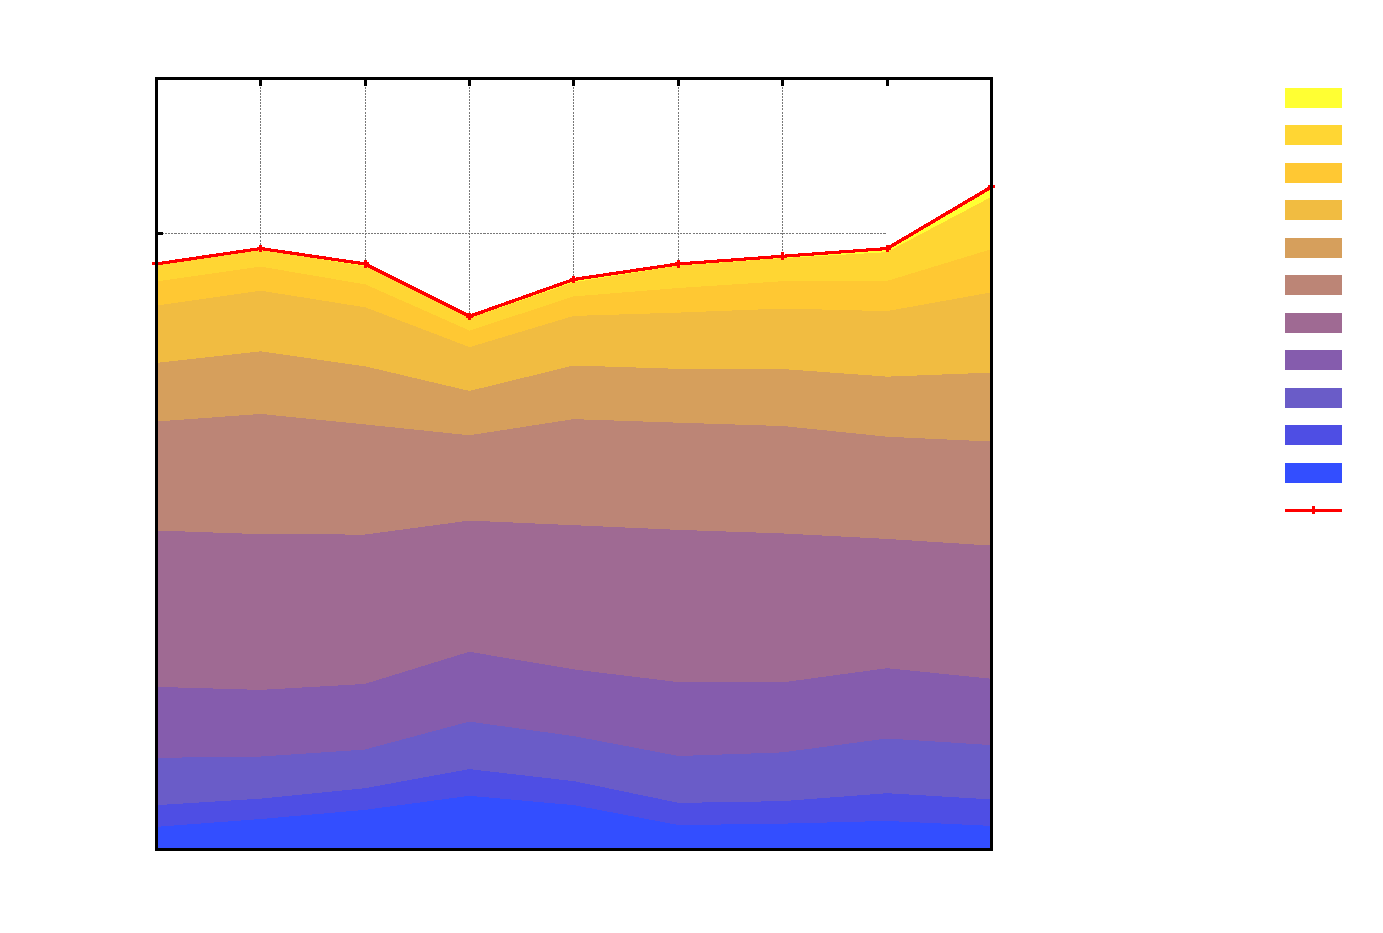
\includegraphics{./plots/house-prices/median-house-prices.eps}}%
    \gplfronttext
  \end{picture}%
\endgroup

\end{sidewaysfigure}
\clearpage
}

An interesting result from the most recent housing survey is `where--to--where' housing market sector transition data among household representatives who moved in the twelve month period before the survey. In order to quality for this sample, a household must either have been: (a) newly formed within one year of the survey, Ie. neither the HRP nor their partner, if present, occupied their most recent permanent accommodation in their names, or (b) continuing households. Where--to--where sector transition data does not include sitting/protected tenant purchasers (Rent Act 1997).\newline

\item Labour Markets\newline

One of the latest comprehensive public analyses of the UK labour market at the time of writing appears to be the ONS statistical bulletin \textit{UK Labour Market, 15 July 2015}. Statistics in this bulletin were derived from surveys of a subset of all households and firms.\newline

As of the period March--May 2015, the total number of people in employment was found to be $30.98$ million. The total number of economically active persons was found to be $32.84$ million. The total number of unemployed people was $1.85$ million. $9.02$ million of $40.7$ million people aged $16$--$64$ were found to be economically inactive ($22.2\%$ or about $1$ in $5$ of the UK population aged $16$--$65$). Of this workforce, $22.7$ million people were found to work full--time hours and $8.3$ million were found to work part--time hours.  Survey participants in employment self--classified their employment status as either part--time or full--time.  Of those who classified themselves as working full--time hours, $86\%$ were regular full--time employees and $14\%$ were self--employed. Of those who classified themselves as working part--time hours, $83\%$ were regular part--time employees and $16\%$ (rounded figures) were self--employed. Of all persons in employment, $85\%$ were employees and $14\%$ were self--employed. A small minority of employees (less than $1\%$) were unpaid family workers ($0.35\%$) or persons that were enrolled on government sponsored training and support programs ($0.32\%$). $6.4\%$ of non self--employed people were found to be working in temporary positions: $5.4\%$ of all persons who were in any form of employment. Of persons who were in temporary employment, almost exactly one in three of these reported that they worked in a temporary position because they could not secure a permanent position. $23\%$ indicated that they favoured a temporary position because they did not want permanent employment. About $15\%$ of all persons who worked part--time hours indicated that they did so because they could not find a full--time position. A majority of persons (over 2 in 3, $68\%$) who worked part--time hours indicated that they did so because they did not want a full--time position. $12.5\%$ of those who worked part--time hours were in education or at school, and about $2.6\%$ indicated that they worked part--time hours on account of illness or disability\footnote{\textit{A01: Summary of labour market statistics}, \textit{Full-time, part-time and temporary workers: People by Full-time, part-time and temporary workers (seasonally adjusted)}, ONS, July 15 2015.}.\newline

About one quarter ($24.2\%$) of all persons aged $16$--$17$ were in employment. Of all economically active young persons aged $16$--$17$, just under 1 in 3 ($29.6\%$) were unemployed (all figures seasonally adjusted). Just under 2 in 3 ($65.6\%$) of young persons aged $16$--$17$ were economically inactive. The \textit{UK Labour Market} survey considers persons that are in full-time eduction to be non--economically inactive only if they do not hold part--time jobs (in which case they are classed as employed) or if they are looking for for part--time employment (in which case they are classed as unemployed). About two thirds ($60.7\%$) of all persons aged $18$--$24$ were in employment. Of all economically active young persons aged $18$--$24$, about 3 in 20 ($14.2\%$) were unemployed. Just under 1 in 3 ($29.3\%$) of young persons aged $18$--$24$ were economically inactive. About four fifths ($80.7\%$) of all persons aged $25$--$34$ were in employment. Of all economically active persons aged $25$--$34$, $5.2\%$ were unemployed. About 3 in 20 ($14.9\%$) of all persons aged $25$--$34$ were economically inactive. Just over four fifths ($83.6\%$) of all persons aged $35$--$49$ were in employment. Of all economically active persons aged $35$--$49$, $3.8\%$ were unemployed. $13.1\%$ of all persons aged $35$--$49$ were economically inactive. Just under 7 in 10 ($69.1\%$) of all persons aged $50$--$64$ were in employment. Of all economically active persons aged $50$--$64$, $3.5\%$ were unemployed. Just over a quarter ($28.4\%$) of all persons aged $50$--$64$ were economically inactive. Finally, about 1 in 10 ($10.1\%$) of all persons aged $65+$ were in employment. Of all economically active persons aged $65+$, $1.7\%$ were unemployed. Just under 9 in 10 ($89.7\%$) of all persons aged $65+$ were economically inactive\footnote{\textit{A01: Summary of labour market statistics}, \textit{Labour market by age group: People by economic activity and age (seasonally adjusted)}, ONS, July 15 2015.}.\newline

Of all men aged 16--64, $83\%$ were found to be economically active and $78.1\%$ held a form of employment (of men aged 16--64 who were economically active, $94\%$ held some form of employment). Slightly under 1 in 5 ($17\%$) were found to be economically inactive. $72.7\%$ of all women aged 16--64 were found to be economically active and $68.7\%$ of all such women were in employment ($94\%$ of all women aged 16--64 who were economically active held some form of employment). Just over 1 in 4 ($27.3\%$) of women aged 16--64 were economically inactive\footnote{\textit{Labour Force Survey Summary:  People by economic activity for those aged 16 and over and those aged from 16 to 64 (seasonally adjusted)}, ONS, July 15 2015.}. Women aged 16--64 are accordingly less likely to be economically active then men, but the proportion of economically active employed men is the same as the proportion of economically active employed women.\newline

The size of the public sector workforce by headcount was $5.372$ million as of the first quarter of $2015$. The UK public sector workforce is defined to be the workforce employed by central government, local government and/or public corporations. The UK private sector workforce is defined to be the total workforce minus the size of the public sector workforce. The largest public sector employer (by a narrow margin) is the UK National Health Service, which as of March 2015 employed about $29.6\%$ of the public sector workforce. The next largest public sector employer is the education sector, which was found to employ about $28.2\%$ of the public sector workforce. Public administrators who were not civil servants accounted for $11.2\%$ of all public sector employees. The civil service accounted for $8.2\%$. Smaller public sector employers included non--NHS social health services ($4.7\%$), policing ($4.7\%$), army ($3.0\%$), construction ($0.7\%$) and other bodies including publicly owned financial institutions ($9.9\%$). Note that these percentages do not sum to $100\%$ because the statistics from which they were sourced were individually seasonally adjusted.\newline

Of the combined public sector workforce, central government employment accounted for $54.2\%$ of employees ($2.909$ million), local government accounted for $42.5\%$ ($2.283$ million), and public corporations accounted for the remainder ($180$k, $3.4\%$). The size of the private sector workforce was $25.681$ million\footnote{\textit{Public Sector Employment, Q1 2015}, ONS, June 15.}.\newline

Of all public sector employees who worked in central government, $86.4\%$ held full--time equivalent (FTE) positions. Of public sector local government employees, $76\%$ were found to hold full-time positions. Across all of government, $81.6\%$ of public sector employees had full--time positions. In public sector corporations ($95\%$) and in the civil service ($92.3\%$) almost all employees worked full--time (seasonally adjusted, Q1 2015)\footnote{\textit{Public Sector Employment, Q1 2015}, ONS, July 15 2015.}.\newline

A detailed distribution of workforce jobs by sector is available in the data tables accompanying the ONS \textit{UK Labour Market}. Note that workforce jobs and employment are distinct measurements. Employment rates refer to the number of people who do or do not have jobs, whereas workforce jobs refer to filled positions, and some persons may hold more than one job concurrently. The distribution of workforce jobs as of March 2015 was found to be as follows: $1.21\%$ of workforce jobs were in agriculture or forestry or fishing, $0.22\%$ were in mining and quarrying activities, $7.85\%$ were in manufacturing activities, $0.38\%$ were in electricity or gas or steam services or jobs that related to air conditioning supplies, $0.59\%$ were in the business of water supply, sewerage or waste processing services, $6.31\%$ were in construction, $14.7\%$ were in motor vehicle repair or wholesale or retail trade activities, $4.7\%$ related to transport and storage, $6.7\%$ related to accommodation and hotels or food services, $4.0\%$ were in information and communication businesses, $3.4\%$ were in financial and insurance businesses, $1.6\%$ related to real estate, $8.8\%$ were in professional scientific and technical activities, $8.3\%$ were in administration and support services, $4.5\%$ were in public administration or army or police or social security activities, $8.7\%$ related to education, $12.5\%$ were in the National Health Service or social work or health businesses, $2.9\%$ were in arts or entertainment activities, $0.2\%$ worked in private households and $2.6\%$ were not classified by any of the previous categories (figures seasonally adjusted).\footnote{\textit{Workforce jobs by industry (seasonally adjusted)},\\ \textit{A01: Summary of labour market statistics}, ONS, July 15 2015.}\newline

Of all persons who were found to be in employment, $1.6\%$ indicated that they usually worked fewer than 6 hours per week. $6.3\%$ usually worked between 6 and 15 hours per week and $7.9\%$ usually worked up to 15 hours per week. About 1 in 5 ($19.9\%$) of employed persons usually worked between 16 and 30 hours weekly, and just over 1 in 4 worked not more than 30 hours. Over half of all people in employment ($52.3\%$) indicated that they usually worked between 31 and 45 hours weekly and just over 4 in 5 ($80.1\%$) worked up to 45 hours. In particular, about 1 in 5 employed persons usually worked more than 45 hours per week.\newline

Of people who were in employment and who were regular employees (not self--employed), $1.1\%$ indicated that they usually worked fewer than 6 hours per week. $5.8\%$ of regular employees worked between 6 and 15 hours per week and $6.9\%$ usually worked not more than 15 hours. About 1 in 5 regular employees ($19.6\%$) usually worked between 16 and 30 hours per week, and over a quarter ($26.5\%$) of them usually worked no more than 30 hours. Over half of all regular employees ($54.9\%$) worked more than 30 weekly but less than 45 hours. The remainder, somewhat less than 1 in 5 regular employees, said that they typically worked over 45 hours per week.\newline

In the extremes, self--employed people tended to work significantly longer hours than regular employees. $4.0\%$ of self--employed persons usually worked fewer than 6 hours per week, $8.3\%$ usually worked 6--15 hours per week ($12.3\%$ usually worked up to 15 hours per week), about 1 in 5 ($21.9\%$) usually worked 16--30 hours per week (just over 1 in 3, $34.2\%$ worked up to 30 hours per week), over a third ($37.3\%$) usually worked 31--45 hours per week, and over a quarter ($28.5\%$) tended to work in excess of 45 hours weekly (weekly hours are all seasonally adjusted figures)\footnote{\textit{Usual weekly hours of work (all in employment): People by usual weekly hours (seasonally adjusted)},\\ \textit{A01: Summary of labour market statistics}, ONS, July 15 2015.}.\newline

The \textit{UK Labour Market} survey found that the average period (duration) of contiguous unemployment among UK citizens tends to be short. Among older persons in the workforce (in particular, those aged $50+$ years), it can be said that if unemployment lasts for longer than 6 months then there is a likelihood that it will last for over 2 years. This outcome is less marked among young persons in the UK workforce, but it is the case among middle--aged economically active unemployed persons that the two durations of unemployment accounting for the largest number of surveyed persons were those (a) lasting up to 6 months and (b) lasting over two years. Across all age groups except those who were very young (in particular, those who were so young that there is very little scope for them to have been unemployed for more than 2 years: UK labour market statistics do not include persons aged under 16) it tended to be the case that the number of economically active persons who had experienced unemployment for 6--12 months was similar to the number of economically active persons who had experienced unemployment for between 1--2 years.\footnote{\textit{Unemployment by age and duration: People duration of unemployment by age},\\ \textit{A01: Summary of labour market statistics}, ONS, July 15 2015.}\newline

Of all economically active people aged 16--64 who were unemployed at the time of the survey, over a half of these ($53.1\%$) had been unemployed for up to 6 months ($46.9\%$ had been unemployed for 6+ months). $16.2\%$ of economically active unemployed 16--64 year olds had been unemployed for more than six months and less than one year ($30.7\%$ had been unemployed for at least 1 year). A similar figure, $13.8\%$, had been unemployed for between 1 and 2 years ($16.9\%$ had been unemployed for more than two years).\footnote{Ibid.}\newline

These observations can be broken down further by age group. Of economically active people in the youngest age bracket 16--17, over three quarters ($76.6\%$) of these had been unemployed for not more than one half of one year ($23.4\%$ had been unemployed for more than 6 months). Over 1 in 10 ($13.2\%$) had been unemployed for 6--12 months ($10.2\%$ had been unemployed for more than 12 months)\footnote{Ibid.}. Of economically active unemployed persons aged 18--24, almost exactly 6 in 10 ($59.999\%$) had been unemployed for a period lasting not more than half a year ($40.0\%$ had been unemployed for longer than six months).\newline

In recent times, redundancies in the UK labour market have tended to be relatively rare in comparison to the overall size of the workforce. Employees who are classified as redundant with respect to the following statistics include employees who accepted voluntary redundancies and those who were subject to compulsory redundancies. UK workforce redundancy data is sourced from the Labour Force Survey (LFS). In order to be classified as redundant by this survey, a participant must have experienced compulsory of voluntary redundancy either in the month containing the reference week of the LFS sample or at any time in the two calender months preceding it. This includes the possibility that a survey participant experienced two or more redundancies within that timeframe. The survey participant need not have found other employment at the moment their survey response\footnote{\textit{Guide to Redundancies}, ONS, 14 November 2012.}. ONS statistics quote redundancy statistics as `redundancies per thousand employees'. This measurement is calculated as the fraction of employees who indicated that they had experienced redundancy in the most recent 3 month timeframe (according to the above criteria) divided by the total number of employees in the previous quarter\footnote{\textit{Redundancies, levels and rates (seasonally adjusted)},\\ \textit{A01: Summary of labour market statistics}, ONS, July 15 2015.}.\newline

118--thousand redundancies were reported in the period March--May 2015. With respect to the total number of employees in the previous quarter, $4.5$ of 1000 employees experienced redundancy. The rate of redundancy is significantly higher among men than women. LFS data indicated that 70--thousand men had experienced redundancy in this period, about 5.3 per 1000 employee men from the previous quarter. 48--thousand women had experienced redundancy in the same timeframe, about 3.7 per 1000 employee women from the previous quarter (all figures are seasonally adjusted)\footnote{Ibid.}.\newline

With respect to the same 3-month sliding window timeframe, the peak redundancy period for UK employees in the last decade was the 3--month period ending April 2009, at which point 311--thousand employees has been made subject to redundancy (12.2 per thousand employees from the previous quarter, 210--thousand men, 16.2 of every 1000 employee men; and 101--thousand women, 8.1 of every 1000 employee women at that time). This was a period of significantly elevated redundancies in the UK workforce: 150 $\pm$ 50--thousand redundancies per 3--month interval is representative of the UK redundancy rate at almost all other times since 1995. The lowest rate of redundancy was the 3--month period ending September 2014, at which point 91--thousand employees had been made subject to redundancy (3.5 per thousand employees from the previous quarter, 45--thousand men, 3.5 of every 1000 employee men; and 45--thousand women, 3.6 of every 1000 employee women at that time)\footnote{Ibid.}.\newline 

Estimates of the distribution and levels of UK weekly/hourly and annualized earnings (per employee) are published in the ONS \textit{Annual Survey of Hours and Earnings} (the `ASHE') data tables. At the time of writing, the most recent edition of the ASHE that includes 2014 earnings statistics is the ONS \textit{Annual Survey of Hours and Earnings -- 2014 Provisional Results} edition\footnote{\textit{Annual Survey of Hours and Earnings - 2014 Provisional Results}, ONS, 19 November 2014:\\ \code{http://www.ons.gov.uk/ons/rel/ashe/annual-survey-of-hours-and-earnings/index.html}}.\newline

ASHE data is sourced from a $1\%$ sample of HM Revenue and Customs PAYE (Pay as You Earn) records. This data includes hourly/weekly remuneration statistics as well as annualized estimations of the same. ASHE statistics refer to remunerated UK employees only, not self--employed individuals or employees who did not collect pay during the sample reference period. Hourly and weekly statistics refer to UK employees who (a) received adult levels of remuneration and who (b) were not affected by leave or absence during the survey period. Annualized statistics are aligned to UK tax years (ending in April each calender year) and refer to employees who received adult levels of pay and who had not changed or started their existing job for at least one year (whether or not their gross pay was affected by absence during that year). Almost all statistics in this survey have a variation coefficient (100 times the standard error divided by the statistic value) of less than $5\%$. Statistics for 2014 in this edition are provisional; statistics for 2013 are not provisional.\footnote{\textit{Guide to time series from the Annual Survey of Hours and Earnings (ASHE)}, Ibid.}\newline

In 2013 among all employees, median annual gross earnings were $\pounds 21,837$ per annum ($\pounds 415.30$ median gross weekly earnings per employee, median $\pounds 11.59$ per hour gross). Among males this was $\pounds 27,151$ per annum ($\pounds 507.80$ gross weekly, $\pounds 12.96$ per hour gross). Among females this was $\pounds 16,972$ ($\pounds 327.20$ gross weekly, $\pounds 10.32$ per hour gross). In 2014 among all employees, median annual gross earnings were $\pounds 22,044$ per annum ($\pounds 417.90$ median gross weekly earnings per employee, median $\pounds 11.61$ per hour). Among males this was $\pounds 27,162$ per annum ($\pounds 506.70$ gross weekly, median $\pounds 12.92$ per hour). Among females this was $\pounds 17,103$ per annum ($\pounds 330.30$ gross weekly, $\pounds 10.37$ per hour).\footnote{\textit{All employees' pay and paid hours by sex, United Kingdom, April 1997 - 2014}, \\ \textit{Annual Survey of Hours and Earnings - 2014 Provisional Results}, ONS, 19 November 2014.}\newline

However, in the extremes, the distribution of UK employee weekly earnings has been heterogeneous. A significant number of employees earned more than double or less than one--third of the observed median gross weekly pay rate. In particular, around $80\%$ of all employees secured weekly earnings that were within $30$--$240\%$ of the median rate and around $50\%$ of all employees secured weekly earnings that were within $60$--$150\%$ of the median.\newline

In 2013, $10\%$ of all employees (who received adult levels of remuneration and so on, as above) received less than $29.9\%$ of median gross weekly earnings and $25\%$ earned less than $60.4\%$. $25\%$ earned more than $155\%$ of the median amount per week and $10\%$ earned more than $219\%$ (namely, over double) the median amount. In 2014 provisionally: $10\%$ of all employees earned less than $30.0\%$ of median gross weekly earnings, 1 in 4 employees earned less than $60.3\%$ of the median, 1 in 4 earned more than $154\%$ of the median and 1 in 10 earned more than $218\%$ of the median. In 2013 among full-time employees (classified as above), 1 in 10 earned less than $55.6\%$ of the median weekly amount (of gross earnings by full--time employees), 1 in 4 earned less than $71.1\%$ of the median, 1 in 4 earned more than $141\%$ of the median and 1 in 10 earned more than $197\%$ of the median. Among part--time employees, 1 in 10 earned less than $31.2\%$ of the median weekly amount (of gross earnings by part--time employees), 1 in 4 earned less than $62\%$ of the median amount, 1 in 4 earned more than $154\%$ of the median amount and 1 in 10 earned more than $245\%$ of the median. Provisional results for 2014 indicate that this distribution was largely the same one year later\footnote{\textit{Distribution of gross weekly pay, United Kingdom, April 1997 - 2014}, \\ \textit{Annual Survey of Hours and Earnings - 2014 Provisional Results}, ONS, 19 November 2014.}.\newline

\afterpage{
\begin{sidewaysfigure}[ht]
% GNUPLOT: LaTeX picture with Postscript
\begingroup
  \fontfamily{Serif}%
  \selectfont
  \makeatletter
  \providecommand\color[2][]{%
    \GenericError{(gnuplot) \space\space\space\@spaces}{%
      Package color not loaded in conjunction with
      terminal option `colourtext'%
    }{See the gnuplot documentation for explanation.%
    }{Either use 'blacktext' in gnuplot or load the package
      color.sty in LaTeX.}%
    \renewcommand\color[2][]{}%
  }%
  \providecommand\includegraphics[2][]{%
    \GenericError{(gnuplot) \space\space\space\@spaces}{%
      Package graphicx or graphics not loaded%
    }{See the gnuplot documentation for explanation.%
    }{The gnuplot epslatex terminal needs graphicx.sty or graphics.sty.}%
    \renewcommand\includegraphics[2][]{}%
  }%
  \providecommand\rotatebox[2]{#2}%
  \@ifundefined{ifGPcolor}{%
    \newif\ifGPcolor
    \GPcolortrue
  }{}%
  \@ifundefined{ifGPblacktext}{%
    \newif\ifGPblacktext
    \GPblacktexttrue
  }{}%
  % define a \g@addto@macro without @ in the name:
  \let\gplgaddtomacro\g@addto@macro
  % define empty templates for all commands taking text:
  \gdef\gplbacktext{}%
  \gdef\gplfronttext{}%
  \makeatother
  \ifGPblacktext
    % no textcolor at all
    \def\colorrgb#1{}%
    \def\colorgray#1{}%
  \else
    % gray or color?
    \ifGPcolor
      \def\colorrgb#1{\color[rgb]{#1}}%
      \def\colorgray#1{\color[gray]{#1}}%
      \expandafter\def\csname LTw\endcsname{\color{white}}%
      \expandafter\def\csname LTb\endcsname{\color{black}}%
      \expandafter\def\csname LTa\endcsname{\color{black}}%
      \expandafter\def\csname LT0\endcsname{\color[rgb]{1,0,0}}%
      \expandafter\def\csname LT1\endcsname{\color[rgb]{0,1,0}}%
      \expandafter\def\csname LT2\endcsname{\color[rgb]{0,0,1}}%
      \expandafter\def\csname LT3\endcsname{\color[rgb]{1,0,1}}%
      \expandafter\def\csname LT4\endcsname{\color[rgb]{0,1,1}}%
      \expandafter\def\csname LT5\endcsname{\color[rgb]{1,1,0}}%
      \expandafter\def\csname LT6\endcsname{\color[rgb]{0,0,0}}%
      \expandafter\def\csname LT7\endcsname{\color[rgb]{1,0.3,0}}%
      \expandafter\def\csname LT8\endcsname{\color[rgb]{0.5,0.5,0.5}}%
    \else
      % gray
      \def\colorrgb#1{\color{black}}%
      \def\colorgray#1{\color[gray]{#1}}%
      \expandafter\def\csname LTw\endcsname{\color{white}}%
      \expandafter\def\csname LTb\endcsname{\color{black}}%
      \expandafter\def\csname LTa\endcsname{\color{black}}%
      \expandafter\def\csname LT0\endcsname{\color{black}}%
      \expandafter\def\csname LT1\endcsname{\color{black}}%
      \expandafter\def\csname LT2\endcsname{\color{black}}%
      \expandafter\def\csname LT3\endcsname{\color{black}}%
      \expandafter\def\csname LT4\endcsname{\color{black}}%
      \expandafter\def\csname LT5\endcsname{\color{black}}%
      \expandafter\def\csname LT6\endcsname{\color{black}}%
      \expandafter\def\csname LT7\endcsname{\color{black}}%
      \expandafter\def\csname LT8\endcsname{\color{black}}%
    \fi
  \fi
  \setlength{\unitlength}{0.0500bp}%
  \begin{picture}(10080.00,11520.00)(2000,0)%
    \gplgaddtomacro\gplbacktext{%
      \csname LTb\endcsname%
      \put(480,6160){\makebox(0,0)[r]{\strut{} 100}}%
      \csname LTb\endcsname%
      \put(480,6656){\makebox(0,0)[r]{\strut{} 200}}%
      \csname LTb\endcsname%
      \put(480,7152){\makebox(0,0)[r]{\strut{} 300}}%
      \csname LTb\endcsname%
      \put(480,7648){\makebox(0,0)[r]{\strut{} 400}}%
      \csname LTb\endcsname%
      \put(480,8144){\makebox(0,0)[r]{\strut{} 500}}%
      \csname LTb\endcsname%
      \put(480,8640){\makebox(0,0)[r]{\strut{} 600}}%
      \csname LTb\endcsname%
      \put(480,9135){\makebox(0,0)[r]{\strut{} 700}}%
      \csname LTb\endcsname%
      \put(480,9631){\makebox(0,0)[r]{\strut{} 800}}%
      \csname LTb\endcsname%
      \put(480,10127){\makebox(0,0)[r]{\strut{} 900}}%
      \csname LTb\endcsname%
      \put(480,10623){\makebox(0,0)[r]{\strut{} 1000}}%
      \csname LTb\endcsname%
      \put(480,11119){\makebox(0,0)[r]{\strut{} 1100}}%
      \csname LTb\endcsname%
      \put(942,5960){\makebox(0,0){\strut{} 1998}}%
      \csname LTb\endcsname%
      \put(1626,5960){\makebox(0,0){\strut{} 2000}}%
      \csname LTb\endcsname%
      \put(2311,5960){\makebox(0,0){\strut{} 2002}}%
      \csname LTb\endcsname%
      \put(2995,5960){\makebox(0,0){\strut{} 2004}}%
      \csname LTb\endcsname%
      \put(3679,5960){\makebox(0,0){\strut{} 2006}}%
      \csname LTb\endcsname%
      \put(4363,5960){\makebox(0,0){\strut{} 2008}}%
      \csname LTb\endcsname%
      \put(5048,5960){\makebox(0,0){\strut{} 2010}}%
      \csname LTb\endcsname%
      \put(5732,5960){\makebox(0,0){\strut{} 2012}}%
      \csname LTb\endcsname%
      \put(6416,5960){\makebox(0,0){\strut{} 2014}}%
      \put(-340,8639){\rotatebox{-270}{\makebox(0,0){\strut{}Gross Annual Earnings (GBP $\pounds$, not adjusted)}}}%
      \put(3508,5660){\makebox(0,0){\strut{}Year}}%
      \put(3508,11719){\makebox(0,0){\strut{}Employee Earnings, Percentiles, Full--Time}}%
      \put(3508,11419){\makebox(0,0){\strut{}(Tenth, $25\%$, $50\%$, $75\%$ and Nintieth Percentile Boundaries)}}%
      \put(6800,7700){\makebox(0,0)[l]{\strut{}\begin{minipage}[t][][t]{5.5cm}\small
Full--time annual gross non--adjusted employee earnings percentiles. Based on full--time employees receiving adult rates of pay. In this survey, full--time is defined to be more than 30 hours of paid work per week for all professions except teaching, for which more than 25 hours of paid work per week qualifies as full--time. Source: {\it Distribution of gross weekly pay, United Kingdom, April 1997--2014 (Full--Time Respondents)}, {\it Annual Survey of Hours and Earnings (ASHE)}, \textit{\it ONS}.
\end{minipage}}}%
    }%
    \gplgaddtomacro\gplfronttext{%
      \csname LTb\endcsname%
      \put(9176,10969){\makebox(0,0)[r]{\strut{}$10\%$ Earned Less Than}}%
      \csname LTb\endcsname%
      \put(9176,10669){\makebox(0,0)[r]{\strut{}$25\%$ Earned Less Than}}%
      \csname LTb\endcsname%
      \put(9176,10369){\makebox(0,0)[r]{\strut{}$50\%$ Earned Less Than}}%
      \csname LTb\endcsname%
      \put(9176,10069){\makebox(0,0)[r]{\strut{}$75\%$ Earned Less Than}}%
      \csname LTb\endcsname%
      \put(9176,9769){\makebox(0,0)[r]{\strut{}$90\%$ Earned Less Than}}%
    }%
    \gplgaddtomacro\gplbacktext{%
      \csname LTb\endcsname%
      \put(480,0){\makebox(0,0)[r]{\strut{} 0}}%
      \csname LTb\endcsname%
      \put(480,620){\makebox(0,0)[r]{\strut{} 50}}%
      \csname LTb\endcsname%
      \put(480,1240){\makebox(0,0)[r]{\strut{} 100}}%
      \csname LTb\endcsname%
      \put(480,1860){\makebox(0,0)[r]{\strut{} 150}}%
      \csname LTb\endcsname%
      \put(480,2480){\makebox(0,0)[r]{\strut{} 200}}%
      \csname LTb\endcsname%
      \put(480,3100){\makebox(0,0)[r]{\strut{} 250}}%
      \csname LTb\endcsname%
      \put(480,3720){\makebox(0,0)[r]{\strut{} 300}}%
      \csname LTb\endcsname%
      \put(480,4340){\makebox(0,0)[r]{\strut{} 350}}%
      \csname LTb\endcsname%
      \put(480,4960){\makebox(0,0)[r]{\strut{} 400}}%
      \csname LTb\endcsname%
      \put(942,-200){\makebox(0,0){\strut{} 1998}}%
      \csname LTb\endcsname%
      \put(1626,-200){\makebox(0,0){\strut{} 2000}}%
      \csname LTb\endcsname%
      \put(2311,-200){\makebox(0,0){\strut{} 2002}}%
      \csname LTb\endcsname%
      \put(2995,-200){\makebox(0,0){\strut{} 2004}}%
      \csname LTb\endcsname%
      \put(3679,-200){\makebox(0,0){\strut{} 2006}}%
      \csname LTb\endcsname%
      \put(4363,-200){\makebox(0,0){\strut{} 2008}}%
      \csname LTb\endcsname%
      \put(5048,-200){\makebox(0,0){\strut{} 2010}}%
      \csname LTb\endcsname%
      \put(5732,-200){\makebox(0,0){\strut{} 2012}}%
      \csname LTb\endcsname%
      \put(6416,-200){\makebox(0,0){\strut{} 2014}}%
      \put(-220,2480){\rotatebox{-270}{\makebox(0,0){\strut{}Gross Annual Earnings (GBP $\pounds$, not adjusted)}}}%
      \put(3508,-500){\makebox(0,0){\strut{}Year}}%
      \put(3508,5260){\makebox(0,0){\strut{}Employee Earnings, Percentiles, Part--Time}}%
      \put(6800,1500){\makebox(0,0)[l]{\strut{}\begin{minipage}[t][][t]{5.5cm}\small
Part--time annual gross non--adjusted employee earnings percentiles. Based on part--time employees receiving adult rates of pay. In this survey, full--time is defined to be less than 30 hours of paid work per week for all professions except teaching, for which more than 25 hours of paid work per week qualifies as full--time. Source: {\it Distribution of gross weekly pay, United Kingdom, April 1997--2014 (Part--Time Respondents)}, {\it Annual Survey of Hours and Earnings (ASHE)}, \textit{\it ONS}.
\end{minipage}}}%
    }%
    \gplgaddtomacro\gplfronttext{%
      \csname LTb\endcsname%
      \put(9176,4810){\makebox(0,0)[r]{\strut{}$10\%$ Earned Less Than}}%
      \csname LTb\endcsname%
      \put(9176,4510){\makebox(0,0)[r]{\strut{}$25\%$ Earned Less Than}}%
      \csname LTb\endcsname%
      \put(9176,4210){\makebox(0,0)[r]{\strut{}$50\%$ Earned Less Than}}%
      \csname LTb\endcsname%
      \put(9176,3910){\makebox(0,0)[r]{\strut{}$75\%$ Earned Less Than}}%
      \csname LTb\endcsname%
      \put(9176,3610){\makebox(0,0)[r]{\strut{}$90\%$ Earned Less Than}}%
    }%
    \gplbacktext
    \put(0,0){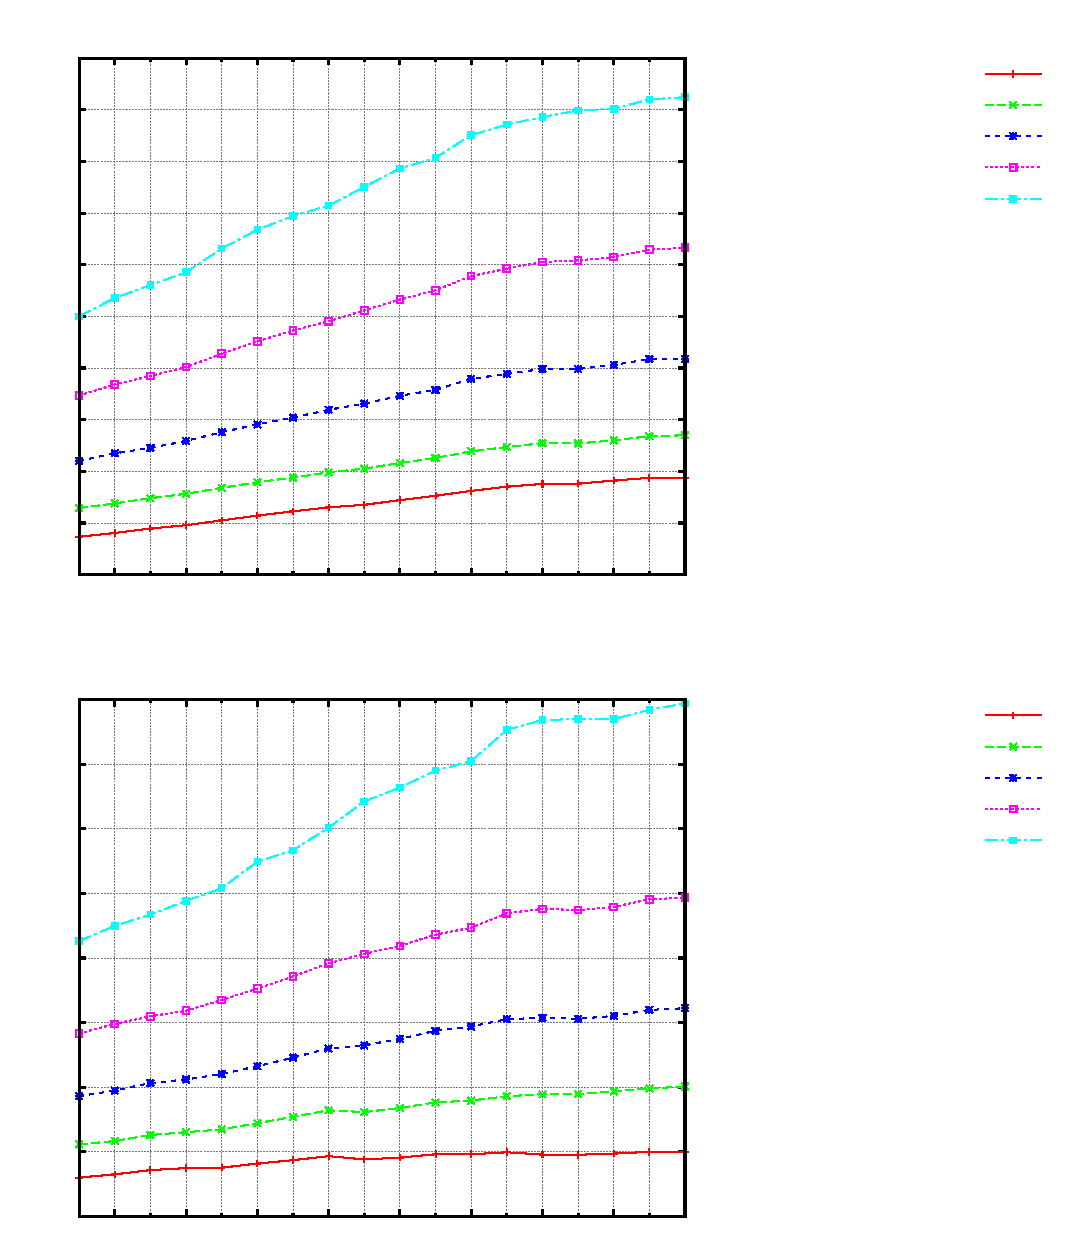
\includegraphics{./plots/wage-percentiles-ftpt/wage-percentiles.eps}}%
    \gplfronttext
  \end{picture}%
\endgroup

\end{sidewaysfigure}
\clearpage
}

\afterpage{
% GNUPLOT: LaTeX picture with Postscript
\begingroup
  \fontfamily{Serif}%
  \selectfont
  \makeatletter
  \providecommand\color[2][]{%
    \GenericError{(gnuplot) \space\space\space\@spaces}{%
      Package color not loaded in conjunction with
      terminal option `colourtext'%
    }{See the gnuplot documentation for explanation.%
    }{Either use 'blacktext' in gnuplot or load the package
      color.sty in LaTeX.}%
    \renewcommand\color[2][]{}%
  }%
  \providecommand\includegraphics[2][]{%
    \GenericError{(gnuplot) \space\space\space\@spaces}{%
      Package graphicx or graphics not loaded%
    }{See the gnuplot documentation for explanation.%
    }{The gnuplot epslatex terminal needs graphicx.sty or graphics.sty.}%
    \renewcommand\includegraphics[2][]{}%
  }%
  \providecommand\rotatebox[2]{#2}%
  \@ifundefined{ifGPcolor}{%
    \newif\ifGPcolor
    \GPcolortrue
  }{}%
  \@ifundefined{ifGPblacktext}{%
    \newif\ifGPblacktext
    \GPblacktexttrue
  }{}%
  % define a \g@addto@macro without @ in the name:
  \let\gplgaddtomacro\g@addto@macro
  % define empty templates for all commands taking text:
  \gdef\gplbacktext{}%
  \gdef\gplfronttext{}%
  \makeatother
  \ifGPblacktext
    % no textcolor at all
    \def\colorrgb#1{}%
    \def\colorgray#1{}%
  \else
    % gray or color?
    \ifGPcolor
      \def\colorrgb#1{\color[rgb]{#1}}%
      \def\colorgray#1{\color[gray]{#1}}%
      \expandafter\def\csname LTw\endcsname{\color{white}}%
      \expandafter\def\csname LTb\endcsname{\color{black}}%
      \expandafter\def\csname LTa\endcsname{\color{black}}%
      \expandafter\def\csname LT0\endcsname{\color[rgb]{1,0,0}}%
      \expandafter\def\csname LT1\endcsname{\color[rgb]{0,1,0}}%
      \expandafter\def\csname LT2\endcsname{\color[rgb]{0,0,1}}%
      \expandafter\def\csname LT3\endcsname{\color[rgb]{1,0,1}}%
      \expandafter\def\csname LT4\endcsname{\color[rgb]{0,1,1}}%
      \expandafter\def\csname LT5\endcsname{\color[rgb]{1,1,0}}%
      \expandafter\def\csname LT6\endcsname{\color[rgb]{0,0,0}}%
      \expandafter\def\csname LT7\endcsname{\color[rgb]{1,0.3,0}}%
      \expandafter\def\csname LT8\endcsname{\color[rgb]{0.5,0.5,0.5}}%
    \else
      % gray
      \def\colorrgb#1{\color{black}}%
      \def\colorgray#1{\color[gray]{#1}}%
      \expandafter\def\csname LTw\endcsname{\color{white}}%
      \expandafter\def\csname LTb\endcsname{\color{black}}%
      \expandafter\def\csname LTa\endcsname{\color{black}}%
      \expandafter\def\csname LT0\endcsname{\color{black}}%
      \expandafter\def\csname LT1\endcsname{\color{black}}%
      \expandafter\def\csname LT2\endcsname{\color{black}}%
      \expandafter\def\csname LT3\endcsname{\color{black}}%
      \expandafter\def\csname LT4\endcsname{\color{black}}%
      \expandafter\def\csname LT5\endcsname{\color{black}}%
      \expandafter\def\csname LT6\endcsname{\color{black}}%
      \expandafter\def\csname LT7\endcsname{\color{black}}%
      \expandafter\def\csname LT8\endcsname{\color{black}}%
    \fi
  \fi
  \setlength{\unitlength}{0.0500bp}%
  \begin{picture}(10080.00,11520.00)(2000,0)%
    \gplgaddtomacro\gplbacktext{%
      \csname LTb\endcsname%
      \put(480,6160){\makebox(0,0)[r]{\strut{} 100}}%
      \csname LTb\endcsname%
      \put(480,6656){\makebox(0,0)[r]{\strut{} 200}}%
      \csname LTb\endcsname%
      \put(480,7152){\makebox(0,0)[r]{\strut{} 300}}%
      \csname LTb\endcsname%
      \put(480,7648){\makebox(0,0)[r]{\strut{} 400}}%
      \csname LTb\endcsname%
      \put(480,8144){\makebox(0,0)[r]{\strut{} 500}}%
      \csname LTb\endcsname%
      \put(480,8640){\makebox(0,0)[r]{\strut{} 600}}%
      \csname LTb\endcsname%
      \put(480,9135){\makebox(0,0)[r]{\strut{} 700}}%
      \csname LTb\endcsname%
      \put(480,9631){\makebox(0,0)[r]{\strut{} 800}}%
      \csname LTb\endcsname%
      \put(480,10127){\makebox(0,0)[r]{\strut{} 900}}%
      \csname LTb\endcsname%
      \put(480,10623){\makebox(0,0)[r]{\strut{} 1000}}%
      \csname LTb\endcsname%
      \put(480,11119){\makebox(0,0)[r]{\strut{} 1100}}%
      \csname LTb\endcsname%
      \put(942,5960){\makebox(0,0){\strut{} 1998}}%
      \csname LTb\endcsname%
      \put(1626,5960){\makebox(0,0){\strut{} 2000}}%
      \csname LTb\endcsname%
      \put(2311,5960){\makebox(0,0){\strut{} 2002}}%
      \csname LTb\endcsname%
      \put(2995,5960){\makebox(0,0){\strut{} 2004}}%
      \csname LTb\endcsname%
      \put(3679,5960){\makebox(0,0){\strut{} 2006}}%
      \csname LTb\endcsname%
      \put(4363,5960){\makebox(0,0){\strut{} 2008}}%
      \csname LTb\endcsname%
      \put(5048,5960){\makebox(0,0){\strut{} 2010}}%
      \csname LTb\endcsname%
      \put(5732,5960){\makebox(0,0){\strut{} 2012}}%
      \csname LTb\endcsname%
      \put(6416,5960){\makebox(0,0){\strut{} 2014}}%
      \put(-340,8639){\rotatebox{-270}{\makebox(0,0){\strut{}Gross Annual Earnings (GBP $\pounds$, not adjusted)}}}%
      \put(3508,5660){\makebox(0,0){\strut{}Year}}%
      \put(3508,11719){\makebox(0,0){\strut{}Employee Earnings, Percentiles, Full--Time}}%
      \put(3508,11419){\makebox(0,0){\strut{}(Tenth, $25\%$, $50\%$, $75\%$ and Nintieth Percentile Boundaries)}}%
      \put(6800,7700){\makebox(0,0)[l]{\strut{}\begin{minipage}[t][][t]{5.5cm}\small
Full--time annual gross non--adjusted employee earnings percentiles. Based on full--time employees receiving adult rates of pay. In this survey, full--time is defined to be more than 30 hours of paid work per week for all professions except teaching, for which more than 25 hours of paid work per week qualifies as full--time. Source: {\it Distribution of gross weekly pay, United Kingdom, April 1997--2014 (Full--Time Respondents)}, {\it Annual Survey of Hours and Earnings (ASHE)}, \textit{\it ONS}.
\end{minipage}}}%
    }%
    \gplgaddtomacro\gplfronttext{%
      \csname LTb\endcsname%
      \put(9176,10969){\makebox(0,0)[r]{\strut{}$10\%$ Earned Less Than}}%
      \csname LTb\endcsname%
      \put(9176,10669){\makebox(0,0)[r]{\strut{}$25\%$ Earned Less Than}}%
      \csname LTb\endcsname%
      \put(9176,10369){\makebox(0,0)[r]{\strut{}$50\%$ Earned Less Than}}%
      \csname LTb\endcsname%
      \put(9176,10069){\makebox(0,0)[r]{\strut{}$75\%$ Earned Less Than}}%
      \csname LTb\endcsname%
      \put(9176,9769){\makebox(0,0)[r]{\strut{}$90\%$ Earned Less Than}}%
    }%
    \gplgaddtomacro\gplbacktext{%
      \csname LTb\endcsname%
      \put(480,0){\makebox(0,0)[r]{\strut{} 0}}%
      \csname LTb\endcsname%
      \put(480,620){\makebox(0,0)[r]{\strut{} 50}}%
      \csname LTb\endcsname%
      \put(480,1240){\makebox(0,0)[r]{\strut{} 100}}%
      \csname LTb\endcsname%
      \put(480,1860){\makebox(0,0)[r]{\strut{} 150}}%
      \csname LTb\endcsname%
      \put(480,2480){\makebox(0,0)[r]{\strut{} 200}}%
      \csname LTb\endcsname%
      \put(480,3100){\makebox(0,0)[r]{\strut{} 250}}%
      \csname LTb\endcsname%
      \put(480,3720){\makebox(0,0)[r]{\strut{} 300}}%
      \csname LTb\endcsname%
      \put(480,4340){\makebox(0,0)[r]{\strut{} 350}}%
      \csname LTb\endcsname%
      \put(480,4960){\makebox(0,0)[r]{\strut{} 400}}%
      \csname LTb\endcsname%
      \put(942,-200){\makebox(0,0){\strut{} 1998}}%
      \csname LTb\endcsname%
      \put(1626,-200){\makebox(0,0){\strut{} 2000}}%
      \csname LTb\endcsname%
      \put(2311,-200){\makebox(0,0){\strut{} 2002}}%
      \csname LTb\endcsname%
      \put(2995,-200){\makebox(0,0){\strut{} 2004}}%
      \csname LTb\endcsname%
      \put(3679,-200){\makebox(0,0){\strut{} 2006}}%
      \csname LTb\endcsname%
      \put(4363,-200){\makebox(0,0){\strut{} 2008}}%
      \csname LTb\endcsname%
      \put(5048,-200){\makebox(0,0){\strut{} 2010}}%
      \csname LTb\endcsname%
      \put(5732,-200){\makebox(0,0){\strut{} 2012}}%
      \csname LTb\endcsname%
      \put(6416,-200){\makebox(0,0){\strut{} 2014}}%
      \put(-220,2480){\rotatebox{-270}{\makebox(0,0){\strut{}Gross Annual Earnings (GBP $\pounds$, not adjusted)}}}%
      \put(3508,-500){\makebox(0,0){\strut{}Year}}%
      \put(3508,5260){\makebox(0,0){\strut{}Employee Earnings, Percentiles, Part--Time}}%
      \put(6800,1500){\makebox(0,0)[l]{\strut{}\begin{minipage}[t][][t]{5.5cm}\small
Part--time annual gross non--adjusted employee earnings percentiles. Based on part--time employees receiving adult rates of pay. In this survey, full--time is defined to be less than 30 hours of paid work per week for all professions except teaching, for which more than 25 hours of paid work per week qualifies as full--time. Source: {\it Distribution of gross weekly pay, United Kingdom, April 1997--2014 (Part--Time Respondents)}, {\it Annual Survey of Hours and Earnings (ASHE)}, \textit{\it ONS}.
\end{minipage}}}%
    }%
    \gplgaddtomacro\gplfronttext{%
      \csname LTb\endcsname%
      \put(9176,4810){\makebox(0,0)[r]{\strut{}$10\%$ Earned Less Than}}%
      \csname LTb\endcsname%
      \put(9176,4510){\makebox(0,0)[r]{\strut{}$25\%$ Earned Less Than}}%
      \csname LTb\endcsname%
      \put(9176,4210){\makebox(0,0)[r]{\strut{}$50\%$ Earned Less Than}}%
      \csname LTb\endcsname%
      \put(9176,3910){\makebox(0,0)[r]{\strut{}$75\%$ Earned Less Than}}%
      \csname LTb\endcsname%
      \put(9176,3610){\makebox(0,0)[r]{\strut{}$90\%$ Earned Less Than}}%
    }%
    \gplbacktext
    \put(0,0){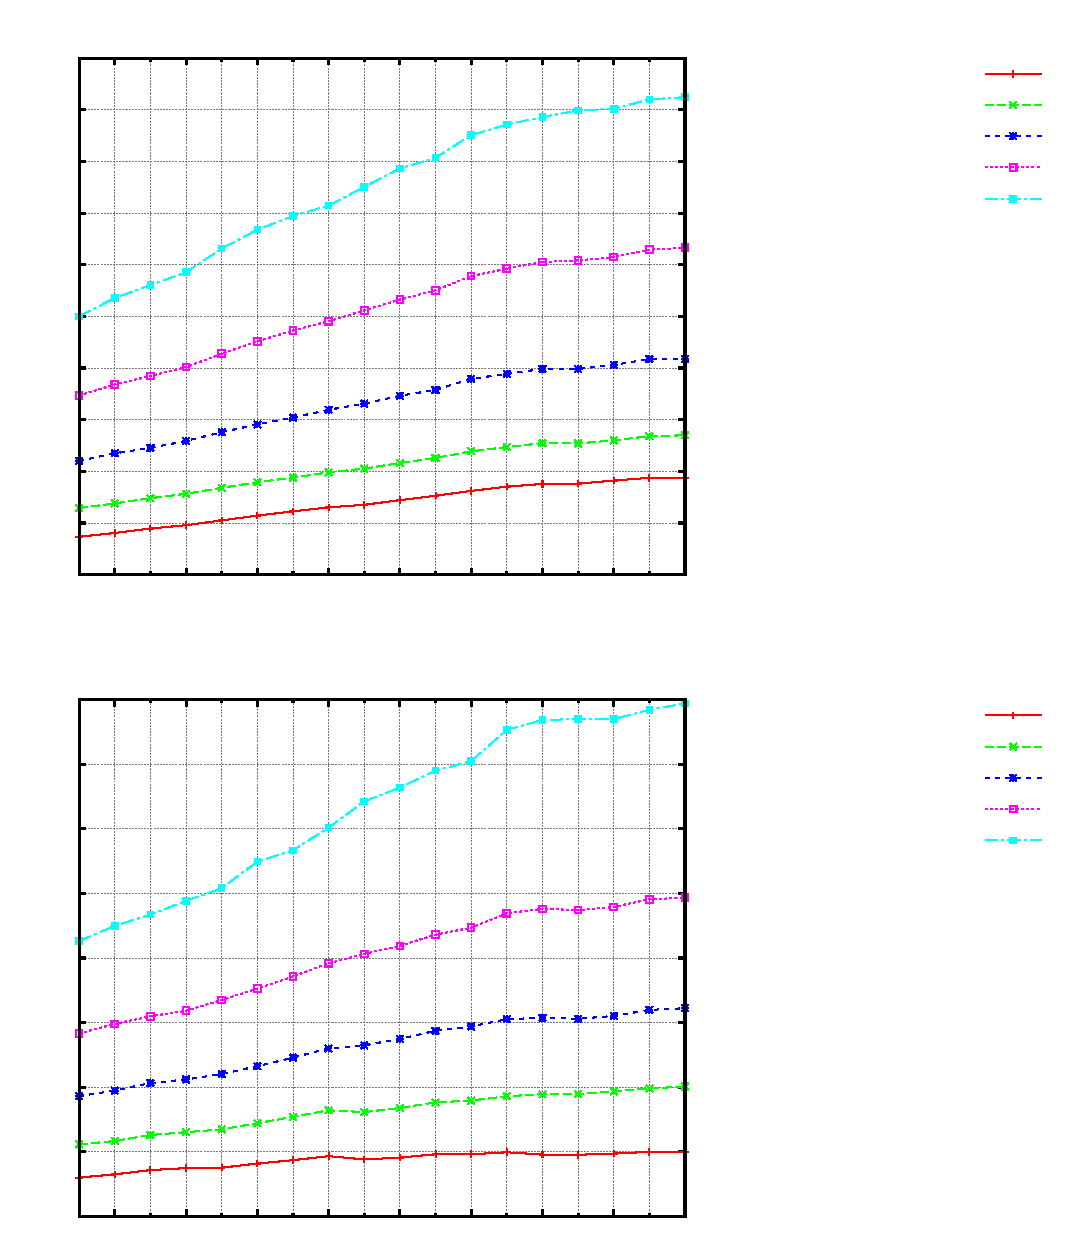
\includegraphics{./plots/wage-percentiles-ftpt/wage-percentiles.eps}}%
    \gplfronttext
  \end{picture}%
\endgroup

\clearpage
}

In 2013 and 2014, survey earnings data indicates that median UK male employees who worked in full--time roles tended to earn about $25\%$ more than their median female counterparts, and median full--time male employees also tend to receive about $\pounds 1.45$ per hour more in remuneration. Among part--time employees in the UK workforce, it is however the case that median female employees tend to earn about $\pounds 0.45$ per hour more than their median male counterparts.\footnote{\textit{Gender pay gap for gross hourly pay (excluding overtime) for full-time and part-time employees, United Kingdom, April 1997 - 2014}, \\ \textit{Annual Survey of Hours and Earnings - 2014 Provisional Results}, ONS, 19 November 2014.}\newline

Concretely: in 2013 among all employees in the UK workforce, the hourly rate of remuneration for median female employees was $19.8\%$ less than the hourly rate received by median male employees. For the average (ie. mean/non--median) employee, female hourly pay rates were $19.1\%$ lower than male rates. Among employees on full-time salaries, median female employees would receive $10.0\%$ less than median male employees and mean female employees would receive $15.7\%$ less. Among part--time employees, median females would receive $5.9\%$ more than males, but mean females would receive $4.6\%$ less than males. In 2014 provisionally: among all employees, median females would receive $19.1\%$ less per hour than males and mean females would receive $17.6\%$ less. Among employees on full--time salaries, median females would receive $9.4\%$ less than median males and mean females would receive $14.2\%$ less than males. Among part--time employees, median females would receive $5.5\%$ more than males and mean females would receive $4.8\%$ less than males.\footnote{Ibid.}\newline

Among regular full--time employees (UK employees who worked at least 30 paid hours per week and who received adult levels of remuneration, or in this survey, employees in teaching professions who received adult levels of remuneration and who worked at least 25 paid hours per week), in 2013 median annual gross earnings per employee were $\pounds 27,011$ per annum ($\pounds 517.40$ median gross weekly earnings per employee, median $\pounds 13.13$ hourly gross). Among male employees in 2013 median gross annual earnings were $\pounds 29,271$ per annum ($\pounds 556.20$ gross weekly, $\pounds 13.73$ hourly gross). Among female employees this was $\pounds 23,584$ ($\pounds 458.90$ gross weekly, $\pounds 12.25$ hourly), just over four fifths ($80.6\%$) of the gross median earnings among males. In 2014 among all employees, median annual gross earnings were $\pounds 27,195$ per annum ($\pounds 518$ median gross weekly earnings per employee, median $\pounds 13.15$ hourly). Among male employees in 2014 this was $\pounds 29,441$ per annum ($\pounds 557.80$ gross weekly, median $\pounds 13.72$ hourly). Among female employees this was $\pounds 23,889$ per annum ($\pounds 461.90$ gross weekly, $\pounds 12.31$ hourly), again just over four fifths of annual gross median earnings among males ($81.1\%$).\footnote{\textit{Full-time employees' pay and paid hours by sex, United Kingdom, April 1997 - 2014, April 1997 - 2014}, \\ \textit{Annual Survey of Hours and Earnings - 2014 Provisional Results}, ONS, 19 November 2014.}\newline

Among part--time employees (UK employees who did not work 30 paid hours per week) comparable annualized and weekly earnings statistics are unavailable. However among all UK part--time employees in 2013, the median hourly remuneration rate was $\pounds 8.26$ (whether or not overtime payments were included in this calculation). Among part--time male employees in the UK workforce, median hourly earnings were $\pounds 7.91$ excluding overtime remuneration and $\pounds 7.90$ including overtime. Among part--time female employees in the UK workforce median hourly earnings were somewhat higher than males at $\pounds 8.37$ per hour (with or without overtime payments). In 2014, provisional median hourly earnings among all part--time UK employees was $\pounds 8.33$ excluding overtime earnings and $\pounds 8.35$ including overtime. Among part--time male employees in 2014, median hourly earnings before and after overtime were $\pounds 8.00$ and $\pounds 8.01$ respectively. Among part--time female employees in 2014 hourly earnings were again somewhat higher than males: median part--time female employees earned $\pounds 8.44$ per hour excluding overtime and $\pounds 8.46$ including overtime.\footnote{\textit{Part-time employees' median hourly pay by sex, United Kingdom, April 1997 - 2014}, \\ \textit{Annual Survey of Hours and Earnings - 2014 Provisional Results}, ONS, 19 November 2014.}\newline

ASHE selected estimates data includes a breakdown of full--time annualized employee pay rates by sector (industry sectors are classified according to the SIC 2007/\textit{Standard Industrial Classification of Economic Activities}\footnote{\textit{UK Standard Industrial Classification of Economic Activities 2007 (SIC 2007)}, \textit{ONS}}). In recent years the UK sector whose employees received the highest median gross annualized earnings was in fact the electricity, gas, steam and air conditioning supply sector (concretely: employees involved in the operation of electricity generation devices including thermal/nuclear/hydro/gas/diesel and renewable generators but not waste incinerators; electricity transmission systems; power lines and meters transmitting electricity from generators to consumers; electricity and/or gas sales and brokerage; producing gas from waste/coal/agriculture by--products; non--long--distance transmission of gas to consumers via networks; and the production and distribution of cooled air, steam, hot water, chilled water or ice for use in cooling\footnote{\textit{Section D, UK SICEA 2007 (Crown Copyright), p.143}} among other professions) followed by median mining and quarrying sector employees\footnote{small/non--confident sample size} (concretely: employees involved in underground or surface mining of hard coal and ligate and alteration of these by various means; underground/surface/underwater mining or quarrying and extraction of crude petroleum oils, bituminous shale, hydrocarbon liquids, iron ores/non--ferrous ores including uranium/thorium, aluminium bauxite, copper, lead, zinc, tin, manganese, chrome, nickel, cobalt and others, and gold/silver/platinum precious metals, clays and kaolin, fertilizer components, salt, sand, limestone, gypsum, chalk, slate and natural gas; gravel pit operation; peat digging; pre--shipment drilling/welling etc.; exploration services and prospecting, and also ancillary extraction site services such as fire--fighters\footnote{\textit{Section B, UK SICEA 2007 (Crown Copyright), p.66}} among other professions) or employees involved in financial and insurance activities (concretely: those involved in central bank activities, including managing state currency, monitoring and regulating money supply, supervising other banks, maintaining the state's international reserves, and government banking; receiving deposits; granting loans, mortgages and credit card services, including at building societies and credit unions; money intermediation by authorized building societies; the activities of various types of holding companies; investment funds and trusts pooling assets on behalf of beneficiaries; life insurance, disability income, accidental death and dismemberment insurance policy underwriters; accident, fire, health, travel, property, vehicle, transport and liability insurance providers; reinsurance; pension funding bodies that supply retirement incomes for their members; administration, supervision and operation of commodity contract/futures/securities/stocks/stock options exchanges; assessment of insurance claims; insurance risk assessment; insurance claim settlements; and for--fee mutual/investment/pension fund management\footnote{\textit{Section K, UK SICEA 2007 (Crown Copyright), p.191}}).\newline

In recent years, after professions in mining/quarrying and the financial sector, the next most profitable full--time professions have been those in information and communications (broadly: employees involved in the publication of books and other like materials including journals, photographic media and software, those who produce and distribute motion pictures/television/videos/music/radio, and also providers of of wired/satellite communications, and computer consultants\footnote{\textit{Section J, UK SICEA 2007 (Crown Copyright), p.183}} among others). At this point, full--time annualized earnings in the next most profitable sectors tend to drop significantly: electricity, gas, steam and air conditioning supply, mining/quarrying, financial services and information and communication sector employees have tended to receive somewhat distinguished rates of remuneration in recent years. In 2013 and in 2014 the next most profitable professions were in professional, scientific and technical activities, and then public administration duties, in that order. Median full--time employees in water supply/sewerage/waste management and remediation activities, construction and education have been the next most well remunerated. Professions receiving the lowest full--time annualized median earnings in recent times have been (a) wholesale and retail traders, repairers of motor vehicles and motorcycles, (b) those in the arts, entertainment and recreation, (c) those in agriculture, forestry and fishing, and (d) those in accommodation and food service activities. Of these, by far the least well--paid median professions were in accommodation and food services\footnote{\textit{full-time employees' pay by industry sector (SIC 2007), United Kingdom, April 2008 - 2014}, \textit{Annual Survey of Hours and Earnings}, ONS}.\newline

In 2014, provisional annual median full--time earnings per employee by sector (ordered highest to lowest) were as follows: electricity, gas, steam and air conditioning supply ($\pounds 37,922$ per annum, not adjusted, among employees working more than 30 hours per week, except in teaching professions, as above), financial and insurance ($\pounds 37,842$ per annum), mining and quarrying ($\pounds 37,539$), information and communication ($\pounds 36,669$), professional, scientific and technical activities ($\pounds 32,781$), public administration, defence and compulsory social security ($\pounds 30,950$), education ($\pounds 29,368$), construction ($\pounds 29,053$), water supply; sewerage, waste management and remediation activities ($\pounds 28,778$), manufacturing ($\pounds 27,763$), transportation and storage ($\pounds 27,716$), real estate activities ($\pounds 25,945$), human health and social work ($\pounds 24,823$), other service activities ($\pounds 23,991$), administrative and support service activities ($\pounds 22,584$), wholesale and retail trade; repair of motor vehicles and motorcycles ($\pounds 21,744$), arts, entertainment and recreation $(\pounds 21,603)$, agriculture, forestry and fishing ($\pounds 21,501$), accommodation and food service activities $(\pounds 16,517)$. In 2013 the corresponding ranking was similar: electricity, gas, steam and air conditioning supply ($\pounds 38,025$ per annum), mining and quarrying ($\pounds 37,589$), financial and insurance ($\pounds 37,330$), information and communication ($\pounds 36,317$), professional, scientific and technical activities $(\pounds 32,800)$, public administration and defence; compulsory social security $(\pounds 30,426)$, water supply; sewerage, waste management and remediation activities $(\pounds 29,389)$, education $(\pounds 29,109)$, construction $(\pounds 28,721)$, transportation and storage $(\pounds 28,008)$, manufacturing $(\pounds 27,433)$, real estate activities $(\pounds 25,452)$, human health and social work activities $(\pounds 24,876)$, other service activities $(\pounds 23,496)$, administrative and support service activities $(\pounds 22,716)$, agriculture, forestry and fishing $(\pounds 21,499)$, wholesale and retail trade; repair of motor vehicles and motorcycles $(\pounds 21,207)$, arts, entertainment and recreation ($\pounds 21,072$), accommodation and food service activities $(\pounds 16,432)$\footnote{Ibid.}.\newline

The highest and lowest extremes of the above distribution can be broken down further (namely, according to granular SIC codes -- note that many professions within each sector receive individual labellings in the standard industrial classification). It should be noted that sample sizes for several of the following professions were small in the most recent edition of the ASHE survey (and accordingly confidence levels in the exact rate or remuneration for these granular professions are lower than is the case for many of the above statistics). In 2014, provisionally the highest paid professions (highest to lowest full--time gross weekly pay, respectively) were: extraction of crude petroleum and natural gas (SIC code 06), manufacture of coke and refined petroleum products (code 19), mining of coal and lignite (code 05), manufacture of tobacco products (code 12), mining support service activities (code 09), financial service activities except insurance and pension funding (code 64), information service activities (code 63), programming and broadcasting activities (code 60), computer programming (code 62), consultancy and related activities and air transportation in that order (code 51). In 2013, the rankings of `mining of coal and lignite' and `manufacture of tobacco products' ware inverted and `financial service activities except insurance and pension funding' was five places lower (and not in the top ten professions). Raw extraction and/or manufacture activities (the top four professions in the above ranking) are estimated to have paid about $\pounds 80$ more gross per week then the next most profitable professions\footnote{\textit{Highest and lowest paid industry groups, United Kingdom, April 2014}, \textit{Annual Survey of Hours and Earnings}, ONS}.\newline

Conversely, at the extreme low end of the pay scale, in 2014 provisionally the least well remunerated full--time professions (lowest to highest full--time gross weekly pay, respectively) were: food and beverage service activities (code 56), accommodation (code 55), residential care activities (code 87), retail trade, except of motor vehicles and motorcycles (code 47), manufacture of wearing apparel (code 14), gambling and betting activities (code 92), fishing and aquaculture (code 03), manufacture of leather and related products (code 15), employment activities (code 78) and other personal service activities (code 96). In 2013 the first six of the above professions received the same ranking and `fishing and agriculture' fell two places behind `employment activities'.\footnote{Ibid.}\newline

The ranks of the above professions can be compared to similar data collected more than a decade ago in 2003. In 2003, \textit{SIC 2007} was yet to be published, so sector classifications were instead based on its predecessor, \textit{SIC 2003}. With respect to this different sector classification (SIC 2003) the ranking of full--time employee professions by sector (employees receiving adult rates of pay in the survey period, in employment in the same job for at least twelve months) was (highest to lowest gross earnings in 2013, respectively): financial intermediation ($\pounds 27,372$ per annum median gross), electricity, gas and water supply ($\pounds 27,343$), mining and quarrying ($\pounds 25,490$), real estate, renting and business activities ($\pounds 24,100$), education ($\pounds 23,026$), public administration and defence, compulsory social security ($\pounds 22,620$), construction ($\pounds 22,490$), transport, storage and communication ($\pounds 21,314$), manufacturing ($\pounds 21,066$), health and social work ($\pounds 19,350$), other community, social and personal service activities ($\pounds 18,634$), wholesale and retail trade; repair of motor vehicles, motorcycles and personal and household goods ($\pounds 17,121$), agriculture, hunting and forestry ($\pounds 15,815$), and then hotels and restaurants ($\pounds 13,293$)\footnote{\textit{Full-time employees' pay by industry sector (SIC 2003), United Kingdom, April 1997 - 2009}, \textit{Annual Survey of Hours and Earnings}, ONS}.\newline

It is commonly assumed that private sector professions are associated with higher gross annual earnings than public sector professions in developed western economies.  This is however not the case for representative full--time employees in the UK (at least, among private sector firms and establishments whose statuses in law are as companies/sole proprietors/partnerships, and public sector entities that are legally regarded as public corporations, central government agencies and local authorities).  Median public sector professions have been associated with significantly higher annual gross earnings than private sector professions since at least the turn of the millennium in the UK. When comparing median gross annual earnings between public and private sector full--time professions, median public sector employees have tended to receive between (around) $7$--$15\%$ more per annum than their peers in the private sector. Since 2010, the difference has been closer to $15\%$ per annum. Excluding overtime remuneration, median hourly earnings per employee have been between about $20$--$30\%$ higher for public sector full--time employees than their private sector peers since comparable records began in 1997, and since 2010 public sector full--time employees have attracted about $30\%$ more per hour excluding overtime. These figures are with respect to full--time employees paid for not less than 30 hours per week (except teaching professions) and annual earnings are based on employees who had been in the same job for at least a year, as above\footnote{\textit{Public / Private sector full-time employees' pay by sex, United Kingdom, April 1997 - 2014}, \textit{Annual Survey of Hours and Earnings}, ONS}.\newline

Among female full--time employees, the public/private sector gross annual earnings difference is twice as pronounced as it is for males: median public sector full--time female employees received about $31$--$35\%$ more than their peers in the private sector per year since 2010 whereas median full--time males in the public sector received around $15\%$ more than their private sector peers in the same period. Prior to 2010 (and since 1997) this annual earnings difference was around $10\%$ for males (public sector males versus private sector males) but was unchanged/similarly high for females: in 1999 the annual earnings gap between public and private sector full--time female employees was $30.5\%$\footnote{Ibid.}.\newline

Concretely: in 2013, among all full--time public sector employees (male and female), median employees collected gross annual earnings of $\pounds 29,487$ per annum ($\pounds 573$ per week median gross, $\pounds 641.50$ gross mean weekly, $\pounds 15.24$ median hourly, $\pounds 15.22$ median hourly excluding overtime earnings). Among private sector full--time employees (of any gender) this was $\pounds 25,797$ per annum ($\pounds 489.90$ median gross weekly, $\pounds 614.40$ mean gross weekly, $\pounds 12.07$ median hourly, $\pounds 11.98$ median hourly excluding overtime earnings). Among male full--time employees, median gross annual earnings in the public sector were $\pounds 32,541$ ($\pounds 623.00$ median gross weekly, $\pounds 714$ mean gross weekly, $\pounds 16.18$ median hourly, $\pounds 16.17$ median hourly excluding overtime). In the private sector median gross full--time make employee earnings were $\pounds 28,201$ ($\pounds 536.10$ median gross weekly, $\pounds 668.70$ mean gross weekly, $\pounds 12.89$ median hourly, $\pounds 12.77$ median hourly excluding overtime earnings). Among full--time female employees in the public sector, median gross annual earnings were $\pounds 27,338$ ($\pounds 535.30$ median gross weekly, $\pounds 585.20$ median gross weekly, $\pounds 14.68$ median hourly, $\pounds 14.63$ median hourly excluding overtime earnings) whereas for private sector full--time female employees, median annual gross earnings were $\pounds 20,698$ ($\pounds 400.90$ median gross weekly, $\pounds 497.40$ mean gross weekly, $\pounds 10.36$ median hourly, $\pounds 10.32$ median hourly excluding overtime)\footnote{\textit{Public / Private sector full-time employees' pay by sex, United Kingdom, April 1997 - 2014}, \textit{Annual Survey of Hours and Earnings}, ONS} (figures not adjusted).\newline

Provisionally, in 2014 the gross annual earnings of median public sector full--time employees was $\pounds 29,785$ per annum ($\pounds 578.60$ per week median gross weekly, $\pounds 643.90$ gross mean weekly, $\pounds 15.45$ median hourly, $\pounds 15.43$ median hourly excluding overtime earnings). Among private sector full--time employees this was $\pounds 26,000$ gross per annum ($\pounds 493.10$ median gross weekly, $\pounds 613.40$ mean gross weekly, $\pounds 12.10$ median hourly, $\pounds 12.00$ median hourly excluding overtime earnings). Among median male full--time employees gross annual public sector earnings were $\pounds 32,890$ ($\pounds 634.90$ median gross weekly, $\pounds 719.60$ mean gross weekly, $\pounds 16.52$ mean hourly, $\pounds 16.48$ median hourly excluding overtime). In the private sector, median male full--time employee earnings were $\pounds 28,420$ ($\pounds 536.20$ median gross weekly, $\pounds 662.90$ mean gross weekly, $\pounds 12.86$ median hourly, $\pounds 12.75$ median hourly excluding overtime). Among full--time female employees in the public sector, median gross annual earnings were $\pounds 27,723$ ($\pounds 539.80$ median gross weekly, $\pounds 588.50$ median gross weekly, $\pounds 14.66$ median hourly, $\pounds 14.66$ median hourly excluding overtime) and for private sector full--time female employees, annual gross earnings were $\pounds 21,025$ ($\pounds 407.30$ median gross weekly, $\pounds 507.20$ mean gross weekly, $\pounds 10.53$ median hourly, $\pounds 10.51$ median hourly excluding overtime)\footnote{Ibid.}.\newline

Annual earnings have tended to be significantly higher in the London region than anywhere else in the UK. In the London region, median gross annual earnings among full--time employees (classified as above) have not been less than $25\%$ higher than gross median earnings among all full--time employees in England at any time since 1999. In 2012, median London region employees earned $30\%$ more than median full--time employees in England as a whole; their earnings have been as much as $40\%$ higher than median full--time employees in Scotland and as much as $50\%$ higher than full--time employees in Wales and Northern Ireland in recent years. Of the major national regions (North--East England, North--West England, Yorkshire and The Humber, the East Midlands, the West Midlands, the East, London, South--East England, South--West England, Wales, Scotland and Northern Ireland), full--time employees in Northern Ireland and Wales have tended to receive the lowest gross annual incomes. In 2014, provisionally the only UK regions whose median employees recieved higher earnings than the national median were the London region and South--East England; employees in all other major regions received less than national median earnings (full--time employees in Scotland earned narrowly less than the UK as a whole)\footnote{\textit{Full-time employees' pay by work region, United Kingdom, April 1997--2014}, \textit{Annual Survey of Hours and Earnings}, ONS}.\newline

In 2014, provisionally the rankings of the major UK regions by gross median full--time employee earnings were as follows (annual earnings highest to lowest): London ($\pounds 35,069$ gross median per annum, $\pounds 660.50$ median gross weekly, $\pounds 17.26$ median hourly), South--East England ($\pounds 28,629$ annually, $\pounds 541.40$ median gross weekly, $\pounds 13.77$ median hourly), (England as a whole: $\pounds 27,487$ annually, $\pounds 523.30$ median gross weekly, $\pounds 13.20$ median hourly; United Kingdom as a whole: $\pounds 27,195$ annually, $\pounds 518$ median gross weekly, $\pounds 13.08$ median hourly) Scotland ($\pounds 27,045$ annually, $\pounds 519.40$ median gross weekly, $\pounds 13.10$ median hourly),
East England ($\pounds 26,830$ annually, $\pounds 505.80$ median gross weekly, $\pounds 12.61$ median hourly), South--West England ($\pounds 25,571$ annually, $\pounds 485$ median gross weekly, $\pounds 12.13$ median hourly), North--West England ($\pounds 25,229$ annually, $\pounds 482.50$ median gross weekly, $\pounds 12.21$ median hourly), the East Midlands ($\pounds 25,027$ annually, $\pounds 477.20$ median gross weekly, $\pounds 11.78$ median hourly),
Yorkshire and The Humber ($\pounds 24,999$ annually, $\pounds 479.10$ median gross weekly, $\pounds 11.78$ median hourly), the West Midlands ($\pounds 24,920$ annually, $\pounds 479.10$ median gross weekly, $\pounds 11.95$ median hourly), North--East England ($\pounds 24,876$ annually, $\pounds 479.10$ median gross weekly, $\pounds 12.13$ median hourly), Wales ($\pounds 24,384$ annually, $\pounds 473.40$ median gross weekly, $\pounds 11.82$ median hourly), and Northern Ireland ($\pounds 24,020$ annually, $\pounds 457.20$ median gross weekly, $\pounds 11.26$ median hourly).\footnote{Ibid.}\newline

In 2013 (not provisional) the regional ranking was as follows (annual earnings highest to lowest): London ($\pounds 35,173$ gross median per annum, $\pounds 654.80$ median gross weekly, $\pounds 17.16$ median hourly), South--East England ($\pounds 28,315$ annually, $\pounds 536.60$ median gross weekly, $\pounds 13.64$ median hourly), (England as a whole: $\pounds 27,372$ annually, $\pounds 520.30$ median gross weekly, $\pounds 13.17$ median hourly; United Kingdom as a whole: $\pounds 27,011$ annually, $\pounds 517.40$ median gross weekly, $\pounds 13.02$ median hourly) East England ($\pounds 26,514$ annually, $\pounds 505.00$ median gross weekly, $\pounds 12.73$ median hourly), Scotland ($\pounds 26,489$ annually, $\pounds 508.70$ median gross weekly, $\pounds 12.87$ median hourly), the West Midlands ($\pounds 25,328$ annually, $\pounds 484.50$ median gross weekly, $\pounds 12.18$ median hourly), South--West England ($\pounds 25,242$ annually, $\pounds 480$ median gross weekly, $\pounds 12.06$ median hourly), North--West England ($\pounds 25,111$ annually, $\pounds 480.80$ median gross weekly, $\pounds 12.20$ median hourly), Yorkshire and The Humber ($\pounds 24,933$ annually, $\pounds 479.10$ median gross weekly, $\pounds 11.91$ median hourly), the East Midlands ($\pounds 24,918$ annually, $\pounds 474.10$ median gross weekly, $\pounds 11.70$ median hourly), North--East England ($\pounds 24,113$ annually, $\pounds 470.10$ median gross weekly, $\pounds 11.93$ median hourly), Wales ($\pounds 24,103$ annually, $\pounds 470.50$ median gross weekly, $\pounds 11.83$ median hourly), and Northern Ireland ($\pounds 23,952$ annually, $\pounds 463.60$ median gross weekly, $\pounds 11.46$ median hourly).\footnote{Ibid.}\newline

It is informative to compare these regional rankings to older earnings statistics, in particular statistics sourced from around the turn of the millennium (namely about 16 years ago, at the time of writing). Employee earnings data from the year 2000 indicates that the extremes of the above regional ranking (in particular in London/South--East England) have remained unchanged for some time. At the turn of the millennium, the only additional region whose median employees earned more than the national median was the East of England. Scottish full--time employees collected the next largest earnings per year at that time also, and the lowest remunerated employees were still in North--East England, Wales and Northern Ireland. Concretely, at the turn of the millennium regional rankings were as follows (annual earnings highest to lowest): London ($\pounds 24,204$ gross median per annum, $\pounds 460$ median gross weekly, $\pounds 11.73$ median hourly), South--East England ($\pounds 19,992$ annually, $\pounds 377.30$ median gross weekly, $\pounds 9.22$ median hourly), (England as a whole: $\pounds 19,107$ annually, $\pounds 364.40$ median gross weekly, $\pounds 8.89$ median hourly), East England ($\pounds 19,020$ annually, $\pounds 358.10$ median gross weekly, $\pounds 8.65$ median hourly), (United Kingdom as a whole: $\pounds 18,848$ annually, $\pounds 359$ median gross weekly, $\pounds 8.76$ median hourly), Scotland ($\pounds 18,029$ annually, $\pounds 338.40$ median gross weekly, $\pounds 8.23$ median hourly), North--West England ($\pounds 17,863$ annually, $\pounds 340.90$ median gross weekly, $\pounds 8.29$ median hourly), South--West England ($\pounds 17,847$ annually, $\pounds 336$ median gross weekly, $\pounds 8.08$ median hourly), the West Midlands ($\pounds 17,812$ annually, $\pounds 340.90$ median gross weekly, $\pounds 8.25$ median hourly), Yorkshire and The Humber ($\pounds 17,503$ annually, $\pounds 335$ median gross weekly, $\pounds 7.95$ median hourly), North--East England ($\pounds 17,430$ annually, $\pounds 329.30$ median gross weekly, $\pounds 8.00$ median hourly), the East Midlands ($\pounds 17,352$ annually, $\pounds 330.80$ median gross weekly, $\pounds 7.91$ median hourly), Wales ($\pounds 17,157$ annually, $\pounds 327.50$ median gross weekly, $\pounds 8.01$ median hourly), and Northern Ireland ($\pounds 16,599$ annually, $\pounds 320.20$ median gross weekly, $\pounds 7.78$ median hourly).\footnote{Ibid.}\newline

\afterpage{
\begin{sidewaysfigure}[ht]
% GNUPLOT: LaTeX picture with Postscript
\begingroup
  \fontfamily{Serif}%
  \selectfont
  \makeatletter
  \providecommand\color[2][]{%
    \GenericError{(gnuplot) \space\space\space\@spaces}{%
      Package color not loaded in conjunction with
      terminal option `colourtext'%
    }{See the gnuplot documentation for explanation.%
    }{Either use 'blacktext' in gnuplot or load the package
      color.sty in LaTeX.}%
    \renewcommand\color[2][]{}%
  }%
  \providecommand\includegraphics[2][]{%
    \GenericError{(gnuplot) \space\space\space\@spaces}{%
      Package graphicx or graphics not loaded%
    }{See the gnuplot documentation for explanation.%
    }{The gnuplot epslatex terminal needs graphicx.sty or graphics.sty.}%
    \renewcommand\includegraphics[2][]{}%
  }%
  \providecommand\rotatebox[2]{#2}%
  \@ifundefined{ifGPcolor}{%
    \newif\ifGPcolor
    \GPcolortrue
  }{}%
  \@ifundefined{ifGPblacktext}{%
    \newif\ifGPblacktext
    \GPblacktexttrue
  }{}%
  % define a \g@addto@macro without @ in the name:
  \let\gplgaddtomacro\g@addto@macro
  % define empty templates for all commands taking text:
  \gdef\gplbacktext{}%
  \gdef\gplfronttext{}%
  \makeatother
  \ifGPblacktext
    % no textcolor at all
    \def\colorrgb#1{}%
    \def\colorgray#1{}%
  \else
    % gray or color?
    \ifGPcolor
      \def\colorrgb#1{\color[rgb]{#1}}%
      \def\colorgray#1{\color[gray]{#1}}%
      \expandafter\def\csname LTw\endcsname{\color{white}}%
      \expandafter\def\csname LTb\endcsname{\color{black}}%
      \expandafter\def\csname LTa\endcsname{\color{black}}%
      \expandafter\def\csname LT0\endcsname{\color[rgb]{1,0,0}}%
      \expandafter\def\csname LT1\endcsname{\color[rgb]{0,1,0}}%
      \expandafter\def\csname LT2\endcsname{\color[rgb]{0,0,1}}%
      \expandafter\def\csname LT3\endcsname{\color[rgb]{1,0,1}}%
      \expandafter\def\csname LT4\endcsname{\color[rgb]{0,1,1}}%
      \expandafter\def\csname LT5\endcsname{\color[rgb]{1,1,0}}%
      \expandafter\def\csname LT6\endcsname{\color[rgb]{0,0,0}}%
      \expandafter\def\csname LT7\endcsname{\color[rgb]{1,0.3,0}}%
      \expandafter\def\csname LT8\endcsname{\color[rgb]{0.5,0.5,0.5}}%
    \else
      % gray
      \def\colorrgb#1{\color{black}}%
      \def\colorgray#1{\color[gray]{#1}}%
      \expandafter\def\csname LTw\endcsname{\color{white}}%
      \expandafter\def\csname LTb\endcsname{\color{black}}%
      \expandafter\def\csname LTa\endcsname{\color{black}}%
      \expandafter\def\csname LT0\endcsname{\color{black}}%
      \expandafter\def\csname LT1\endcsname{\color{black}}%
      \expandafter\def\csname LT2\endcsname{\color{black}}%
      \expandafter\def\csname LT3\endcsname{\color{black}}%
      \expandafter\def\csname LT4\endcsname{\color{black}}%
      \expandafter\def\csname LT5\endcsname{\color{black}}%
      \expandafter\def\csname LT6\endcsname{\color{black}}%
      \expandafter\def\csname LT7\endcsname{\color{black}}%
      \expandafter\def\csname LT8\endcsname{\color{black}}%
    \fi
  \fi
  \setlength{\unitlength}{0.0500bp}%
  \begin{picture}(12960.00,8640.00)%
    \gplgaddtomacro\gplbacktext{%
      \csname LTb\endcsname%
      \put(1100,640){\makebox(0,0)[r]{\strut{} 16000}}%
      \csname LTb\endcsname%
      \put(1100,1380){\makebox(0,0)[r]{\strut{} 18000}}%
      \csname LTb\endcsname%
      \put(1100,2120){\makebox(0,0)[r]{\strut{} 20000}}%
      \csname LTb\endcsname%
      \put(1100,2860){\makebox(0,0)[r]{\strut{} 22000}}%
      \csname LTb\endcsname%
      \put(1100,3600){\makebox(0,0)[r]{\strut{} 24000}}%
      \csname LTb\endcsname%
      \put(1100,4340){\makebox(0,0)[r]{\strut{} 26000}}%
      \csname LTb\endcsname%
      \put(1100,5079){\makebox(0,0)[r]{\strut{} 28000}}%
      \csname LTb\endcsname%
      \put(1100,5819){\makebox(0,0)[r]{\strut{} 30000}}%
      \csname LTb\endcsname%
      \put(1100,6559){\makebox(0,0)[r]{\strut{} 32000}}%
      \csname LTb\endcsname%
      \put(1100,7299){\makebox(0,0)[r]{\strut{} 34000}}%
      \csname LTb\endcsname%
      \put(1100,8039){\makebox(0,0)[r]{\strut{} 36000}}%
      \csname LTb\endcsname%
      \put(1734,440){\makebox(0,0){\strut{} 2000}}%
      \csname LTb\endcsname%
      \put(2763,440){\makebox(0,0){\strut{} 2002}}%
      \csname LTb\endcsname%
      \put(3792,440){\makebox(0,0){\strut{} 2004}}%
      \csname LTb\endcsname%
      \put(4821,440){\makebox(0,0){\strut{} 2006}}%
      \csname LTb\endcsname%
      \put(5850,440){\makebox(0,0){\strut{} 2008}}%
      \csname LTb\endcsname%
      \put(6878,440){\makebox(0,0){\strut{} 2010}}%
      \csname LTb\endcsname%
      \put(7907,440){\makebox(0,0){\strut{} 2012}}%
      \csname LTb\endcsname%
      \put(8936,440){\makebox(0,0){\strut{} 2014}}%
      \put(-10,4339){\rotatebox{-270}{\makebox(0,0){\strut{}Full--Time Employee Earnings}}}%
      \put(280,4339){\rotatebox{-270}{\makebox(0,0){\strut{}(median per employee per annum, gross GBP$\pounds$, not adjusted)}}}%
      \put(5078,-70){\makebox(0,0){\strut{}Year}}%
      \put(5078,8539){\makebox(0,0){\strut{}Regional Employee Earnings (gross annual)}}%
    }%
    \gplgaddtomacro\gplfronttext{%
      \csname LTb\endcsname%
      \put(12056,7889){\makebox(0,0)[r]{\strut{}United Kingdom (Whole)}}%
      \csname LTb\endcsname%
      \put(12056,7589){\makebox(0,0)[r]{\strut{}England (Whole)}}%
      \csname LTb\endcsname%
      \put(12056,7289){\makebox(0,0)[r]{\strut{}North--East England}}%
      \csname LTb\endcsname%
      \put(12056,6989){\makebox(0,0)[r]{\strut{}North--West England}}%
      \csname LTb\endcsname%
      \put(12056,6689){\makebox(0,0)[r]{\strut{}Yorkshire and The Humber}}%
      \csname LTb\endcsname%
      \put(12056,6389){\makebox(0,0)[r]{\strut{}East Midlands}}%
      \csname LTb\endcsname%
      \put(12056,6089){\makebox(0,0)[r]{\strut{}West Midlands}}%
      \csname LTb\endcsname%
      \put(12056,5789){\makebox(0,0)[r]{\strut{}East England}}%
      \csname LTb\endcsname%
      \put(12056,5489){\makebox(0,0)[r]{\strut{}London}}%
      \csname LTb\endcsname%
      \put(12056,5189){\makebox(0,0)[r]{\strut{}South--East England}}%
      \csname LTb\endcsname%
      \put(12056,4889){\makebox(0,0)[r]{\strut{}South--West England}}%
      \csname LTb\endcsname%
      \put(12056,4589){\makebox(0,0)[r]{\strut{}Wales}}%
      \csname LTb\endcsname%
      \put(12056,4289){\makebox(0,0)[r]{\strut{}Scotland}}%
      \csname LTb\endcsname%
      \put(12056,3989){\makebox(0,0)[r]{\strut{}Northern Ireland}}%
    }%
    \put(9600,3300){\makebox(0,0)[l]{\strut{}\small UK Regional Employee Earnings}}%
    \put(9600,1700){\makebox(0,0)[l]{\strut{}\begin{minipage}[t][][t]{6.5cm}\small
Full--time median employee earnings (gross) per annum, not adjusted. Based on full--time employees receiving adult rates of pay. In this survey, full-time is defined to be more than 30 hours of paid work per week for all professions except teaching, for which more than 25 hours of paid work per week qualifies as full--time. Source: {\it Full-time employees' pay by work region, United Kingdom, April 1997--2014}, {\it Annual Survey of Hours and Earnings (ASHE)}, \textit{\it ONS}.
\end{minipage}}}%
    \gplbacktext
    \put(0,0){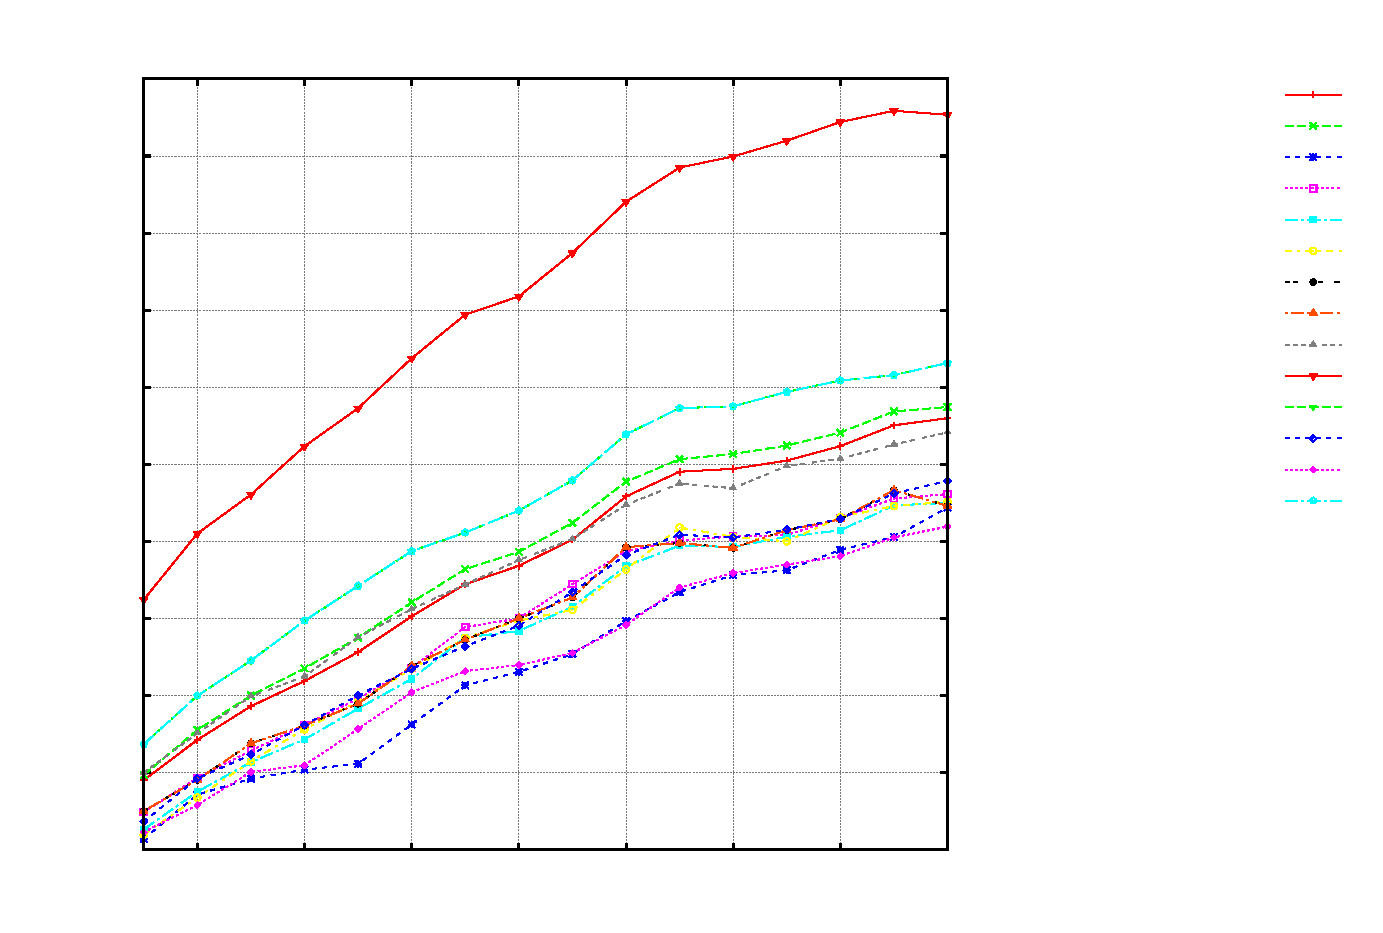
\includegraphics{./plots/regional/regional-rankings.eps}}%
    \gplfronttext
  \end{picture}%
\endgroup

\end{sidewaysfigure}
\clearpage
}

At increased resolution, it can be seen that the local authorities with the highest median annual full--time employee earnings are predominantly based in/around central London, and south--eastern areas close to London, with one exception: in April 2014 Copeland (which is based in the North--West England region, specifically western Cumbria, very far from London) was among the top 3 local authorities whose employees received the highest median annual earnings. Employees in Copeland were among only 3 local authorities for which median full--time gross earnings per week exceeded $\pounds 700$ (a distinction that was shared by the City of London authority, and also Tower Hamlets, London). Median full--time employees in Copeland received more than $\pounds 100$ per week gross than those who worked in Westminster\footnote{\textit{Local authorities with highest and lowest earnings by place of work, Great Britain, April 2014}, \textit{Annual Survey of Hours and Earnings}, ONS}.\newline

The reason for this is likely to be the location of the Sellafield nuclear fuel reprocessing and decommissioning complex, which is based close to Seascale village on the coast of Copeland. This complex employs of the order 10000 persons (which would amount to one in seven persons residing in the whole Copeland region, were it the case that all of these employees lived in Copeland) and is likely to attract specialist engineering professions subject to relatively high rates of remuneration. Many of the local authorities with the lowest earnings (with respect to employee place of work) are not situated in Northern Ireland or Wales. In particular, the local authority with the lowest median rate of full--time employee weekly gross pay is the coastal authority of Rother in South--East England, followed by Torridge in the Cornwall area in far South--West England (low sample size), followed by the coastal authority of Thanet, in the far East of London, and then Arun, another coastal authority south of London. Among Irish (Northern Ireland) and Welsh local authorities, the only authority appearing in the bottom 10 with respect to the above ranking (in April 2014) was Merthyr Tydfil in Wales, which was the tenth lowest\footnote{Ibid.}.\newline

Concretely: with respect to highest median gross weekly earnings among full--time employees, the ten local authorities whose employees (place of work) received the highest rates of remuneration in April 2014 were: the City of London (London region, $\pounds 928$ median gross weekly), Tower Hamlets (London region, $\pounds 900.80$ gross weekly), Copeland (North--West England region, $\pounds 808.20$ gross weekly), Westminster (London region, $\pounds 682.60$ gross weekly), Lambeth (London region, $\pounds 679.80$ gross weekly), Camden (London region, $\pounds 679.40$ gross weekly), Bracknell Forest UA (South--East England region, $\pounds 679.30$ gross weekly), Islington (London region, $\pounds 674.70$ gross weekly), Spelthorne (South--East England region, $\pounds 667.70$ gross weekly, low sample size) and then Southwark (London region, $\pounds 667.60$ gross weekly)\footnote{Ibid.}.\newline

With respect to lowest median gross weekly earnings among full--time employees, the ten local authorities whose employees (place of work) received the lowest rates of remuneration in April 2014 were: Rother (South--East England region, $\pounds 379.3$ median gross weekly), Torridge (South--West England region, $\pounds 390.4$ gross weekly), Thanet (South--East England region, $\pounds 391$ gross weekly), Arun (South--East England region, $\pounds 392.5$ gross weekly), Mansfield (East--Midlands region, $\pounds 395.2$ gross weekly), North East Derbyshire (East--Midlands region, $\pounds 398.3$ gross weekly), Forest Heath (East England region, $\pounds 399.1$ gross weekly), North Norfolk (East England region, $\pounds 402.3$ gross weekly), Melton (East--Midlands region, $\pounds 403$ gross weekly), and then Merthyr Tydfil (Wales, $\pounds 403.1$ gross weekly). These results were subject to low sample sizes.\footnote{Ibid.}.\newline

\afterpage{
\begin{sidewaysfigure}[ht]
% GNUPLOT: LaTeX picture with Postscript
\begingroup
  \fontfamily{Serif}%
  \selectfont
  \makeatletter
  \providecommand\color[2][]{%
    \GenericError{(gnuplot) \space\space\space\@spaces}{%
      Package color not loaded in conjunction with
      terminal option `colourtext'%
    }{See the gnuplot documentation for explanation.%
    }{Either use 'blacktext' in gnuplot or load the package
      color.sty in LaTeX.}%
    \renewcommand\color[2][]{}%
  }%
  \providecommand\includegraphics[2][]{%
    \GenericError{(gnuplot) \space\space\space\@spaces}{%
      Package graphicx or graphics not loaded%
    }{See the gnuplot documentation for explanation.%
    }{The gnuplot epslatex terminal needs graphicx.sty or graphics.sty.}%
    \renewcommand\includegraphics[2][]{}%
  }%
  \providecommand\rotatebox[2]{#2}%
  \@ifundefined{ifGPcolor}{%
    \newif\ifGPcolor
    \GPcolortrue
  }{}%
  \@ifundefined{ifGPblacktext}{%
    \newif\ifGPblacktext
    \GPblacktexttrue
  }{}%
  % define a \g@addto@macro without @ in the name:
  \let\gplgaddtomacro\g@addto@macro
  % define empty templates for all commands taking text:
  \gdef\gplbacktext{}%
  \gdef\gplfronttext{}%
  \makeatother
  \ifGPblacktext
    % no textcolor at all
    \def\colorrgb#1{}%
    \def\colorgray#1{}%
  \else
    % gray or color?
    \ifGPcolor
      \def\colorrgb#1{\color[rgb]{#1}}%
      \def\colorgray#1{\color[gray]{#1}}%
      \expandafter\def\csname LTw\endcsname{\color{white}}%
      \expandafter\def\csname LTb\endcsname{\color{black}}%
      \expandafter\def\csname LTa\endcsname{\color{black}}%
      \expandafter\def\csname LT0\endcsname{\color[rgb]{1,0,0}}%
      \expandafter\def\csname LT1\endcsname{\color[rgb]{0,1,0}}%
      \expandafter\def\csname LT2\endcsname{\color[rgb]{0,0,1}}%
      \expandafter\def\csname LT3\endcsname{\color[rgb]{1,0,1}}%
      \expandafter\def\csname LT4\endcsname{\color[rgb]{0,1,1}}%
      \expandafter\def\csname LT5\endcsname{\color[rgb]{1,1,0}}%
      \expandafter\def\csname LT6\endcsname{\color[rgb]{0,0,0}}%
      \expandafter\def\csname LT7\endcsname{\color[rgb]{1,0.3,0}}%
      \expandafter\def\csname LT8\endcsname{\color[rgb]{0.5,0.5,0.5}}%
    \else
      % gray
      \def\colorrgb#1{\color{black}}%
      \def\colorgray#1{\color[gray]{#1}}%
      \expandafter\def\csname LTw\endcsname{\color{white}}%
      \expandafter\def\csname LTb\endcsname{\color{black}}%
      \expandafter\def\csname LTa\endcsname{\color{black}}%
      \expandafter\def\csname LT0\endcsname{\color{black}}%
      \expandafter\def\csname LT1\endcsname{\color{black}}%
      \expandafter\def\csname LT2\endcsname{\color{black}}%
      \expandafter\def\csname LT3\endcsname{\color{black}}%
      \expandafter\def\csname LT4\endcsname{\color{black}}%
      \expandafter\def\csname LT5\endcsname{\color{black}}%
      \expandafter\def\csname LT6\endcsname{\color{black}}%
      \expandafter\def\csname LT7\endcsname{\color{black}}%
      \expandafter\def\csname LT8\endcsname{\color{black}}%
    \fi
  \fi
  \setlength{\unitlength}{0.0500bp}%
  \begin{picture}(10800.00,8640.00)%
    \gplgaddtomacro\gplbacktext{%
      \csname LTb\endcsname%
      \put(1100,640){\makebox(0,0)[r]{\strut{} 10000}}%
      \csname LTb\endcsname%
      \put(1100,1313){\makebox(0,0)[r]{\strut{} 12000}}%
      \csname LTb\endcsname%
      \put(1100,1985){\makebox(0,0)[r]{\strut{} 14000}}%
      \csname LTb\endcsname%
      \put(1100,2658){\makebox(0,0)[r]{\strut{} 16000}}%
      \csname LTb\endcsname%
      \put(1100,3331){\makebox(0,0)[r]{\strut{} 18000}}%
      \csname LTb\endcsname%
      \put(1100,4003){\makebox(0,0)[r]{\strut{} 20000}}%
      \csname LTb\endcsname%
      \put(1100,4676){\makebox(0,0)[r]{\strut{} 22000}}%
      \csname LTb\endcsname%
      \put(1100,5348){\makebox(0,0)[r]{\strut{} 24000}}%
      \csname LTb\endcsname%
      \put(1100,6021){\makebox(0,0)[r]{\strut{} 26000}}%
      \csname LTb\endcsname%
      \put(1100,6694){\makebox(0,0)[r]{\strut{} 28000}}%
      \csname LTb\endcsname%
      \put(1100,7366){\makebox(0,0)[r]{\strut{} 30000}}%
      \csname LTb\endcsname%
      \put(1100,8039){\makebox(0,0)[r]{\strut{} 32000}}%
      \csname LTb\endcsname%
      \put(1220,440){\makebox(0,0){\strut{} 2004}}%
      \csname LTb\endcsname%
      \put(2763,440){\makebox(0,0){\strut{} 2006}}%
      \csname LTb\endcsname%
      \put(4306,440){\makebox(0,0){\strut{} 2008}}%
      \csname LTb\endcsname%
      \put(5850,440){\makebox(0,0){\strut{} 2010}}%
      \csname LTb\endcsname%
      \put(7393,440){\makebox(0,0){\strut{} 2012}}%
      \csname LTb\endcsname%
      \put(8936,440){\makebox(0,0){\strut{} 2014}}%
      \put(160,4339){\rotatebox{-270}{\makebox(0,0){\strut{}Median Full--Time Earnings (per annum gross, GBP $\pounds$, not adjusted)}}}%
      \put(5158,8709){\makebox(0,0){\strut{}Full--Time Employee Earnings by Age Group}}%
      \put(5158,8439){\makebox(0,0){\strut{}(full-time median annual gross earnings by employee age bracket)}}%
      \put(11000,7200){\rotatebox{-270}{\makebox(0,0){\strut{}Age Bracket}}}%
    \put(9600,1700){\makebox(0,0)[l]{\strut{}\begin{minipage}[t][][t]{5.5cm}\small
Full--time median employee earnings (gross) per annum by age group, not adjusted. Based on full--time employees receiving adult rates of pay. In this survey, full--time is defined to be more than 30 hours of paid work per week for all professions except teaching, for which more than 25 hours of paid work per week qualifies as full--time. Source: {\it Full--time employees' pay by age, United Kingdom, April 2004--2014}, {\it Annual Survey of Hours and Earnings (ASHE)}, \textit{\it ONS}.
\end{minipage}}}%
    }%
    \gplgaddtomacro\gplfronttext{%
      \csname LTb\endcsname%
      \put(9896,7889){\makebox(0,0)[r]{\strut{}18--21}}%
      \csname LTb\endcsname%
      \put(9896,7589){\makebox(0,0)[r]{\strut{}22--29}}%
      \csname LTb\endcsname%
      \put(9896,7289){\makebox(0,0)[r]{\strut{}30--39}}%
      \csname LTb\endcsname%
      \put(9896,6989){\makebox(0,0)[r]{\strut{}40--59}}%
      \csname LTb\endcsname%
      \put(9896,6689){\makebox(0,0)[r]{\strut{}50--59}}%
      \csname LTb\endcsname%
      \put(9896,6389){\makebox(0,0)[r]{\strut{}60+}}%
    }%
    \gplbacktext
    \put(0,0){\includegraphics{./plots/age-wage/earnings-by-age-group.eps}}%
    \gplfronttext
  \end{picture}%
\endgroup

\end{sidewaysfigure}
\clearpage
}

\afterpage{
\begin{sidewaysfigure}[ht]
% GNUPLOT: LaTeX picture with Postscript
\begingroup
  \fontfamily{Serif}%
  \selectfont
  \makeatletter
  \providecommand\color[2][]{%
    \GenericError{(gnuplot) \space\space\space\@spaces}{%
      Package color not loaded in conjunction with
      terminal option `colourtext'%
    }{See the gnuplot documentation for explanation.%
    }{Either use 'blacktext' in gnuplot or load the package
      color.sty in LaTeX.}%
    \renewcommand\color[2][]{}%
  }%
  \providecommand\includegraphics[2][]{%
    \GenericError{(gnuplot) \space\space\space\@spaces}{%
      Package graphicx or graphics not loaded%
    }{See the gnuplot documentation for explanation.%
    }{The gnuplot epslatex terminal needs graphicx.sty or graphics.sty.}%
    \renewcommand\includegraphics[2][]{}%
  }%
  \providecommand\rotatebox[2]{#2}%
  \@ifundefined{ifGPcolor}{%
    \newif\ifGPcolor
    \GPcolortrue
  }{}%
  \@ifundefined{ifGPblacktext}{%
    \newif\ifGPblacktext
    \GPblacktexttrue
  }{}%
  % define a \g@addto@macro without @ in the name:
  \let\gplgaddtomacro\g@addto@macro
  % define empty templates for all commands taking text:
  \gdef\gplbacktext{}%
  \gdef\gplfronttext{}%
  \makeatother
  \ifGPblacktext
    % no textcolor at all
    \def\colorrgb#1{}%
    \def\colorgray#1{}%
  \else
    % gray or color?
    \ifGPcolor
      \def\colorrgb#1{\color[rgb]{#1}}%
      \def\colorgray#1{\color[gray]{#1}}%
      \expandafter\def\csname LTw\endcsname{\color{white}}%
      \expandafter\def\csname LTb\endcsname{\color{black}}%
      \expandafter\def\csname LTa\endcsname{\color{black}}%
      \expandafter\def\csname LT0\endcsname{\color[rgb]{1,0,0}}%
      \expandafter\def\csname LT1\endcsname{\color[rgb]{0,1,0}}%
      \expandafter\def\csname LT2\endcsname{\color[rgb]{0,0,1}}%
      \expandafter\def\csname LT3\endcsname{\color[rgb]{1,0,1}}%
      \expandafter\def\csname LT4\endcsname{\color[rgb]{0,1,1}}%
      \expandafter\def\csname LT5\endcsname{\color[rgb]{1,1,0}}%
      \expandafter\def\csname LT6\endcsname{\color[rgb]{0,0,0}}%
      \expandafter\def\csname LT7\endcsname{\color[rgb]{1,0.3,0}}%
      \expandafter\def\csname LT8\endcsname{\color[rgb]{0.5,0.5,0.5}}%
    \else
      % gray
      \def\colorrgb#1{\color{black}}%
      \def\colorgray#1{\color[gray]{#1}}%
      \expandafter\def\csname LTw\endcsname{\color{white}}%
      \expandafter\def\csname LTb\endcsname{\color{black}}%
      \expandafter\def\csname LTa\endcsname{\color{black}}%
      \expandafter\def\csname LT0\endcsname{\color{black}}%
      \expandafter\def\csname LT1\endcsname{\color{black}}%
      \expandafter\def\csname LT2\endcsname{\color{black}}%
      \expandafter\def\csname LT3\endcsname{\color{black}}%
      \expandafter\def\csname LT4\endcsname{\color{black}}%
      \expandafter\def\csname LT5\endcsname{\color{black}}%
      \expandafter\def\csname LT6\endcsname{\color{black}}%
      \expandafter\def\csname LT7\endcsname{\color{black}}%
      \expandafter\def\csname LT8\endcsname{\color{black}}%
    \fi
  \fi
  \setlength{\unitlength}{0.0500bp}%
  \begin{picture}(10800.00,8640.00)%
    \gplgaddtomacro\gplbacktext{%
      \csname LTb\endcsname%
      \put(1100,640){\makebox(0,0)[r]{\strut{} 10000}}%
      \csname LTb\endcsname%
      \put(1100,1313){\makebox(0,0)[r]{\strut{} 12000}}%
      \csname LTb\endcsname%
      \put(1100,1985){\makebox(0,0)[r]{\strut{} 14000}}%
      \csname LTb\endcsname%
      \put(1100,2658){\makebox(0,0)[r]{\strut{} 16000}}%
      \csname LTb\endcsname%
      \put(1100,3331){\makebox(0,0)[r]{\strut{} 18000}}%
      \csname LTb\endcsname%
      \put(1100,4003){\makebox(0,0)[r]{\strut{} 20000}}%
      \csname LTb\endcsname%
      \put(1100,4676){\makebox(0,0)[r]{\strut{} 22000}}%
      \csname LTb\endcsname%
      \put(1100,5348){\makebox(0,0)[r]{\strut{} 24000}}%
      \csname LTb\endcsname%
      \put(1100,6021){\makebox(0,0)[r]{\strut{} 26000}}%
      \csname LTb\endcsname%
      \put(1100,6694){\makebox(0,0)[r]{\strut{} 28000}}%
      \csname LTb\endcsname%
      \put(1100,7366){\makebox(0,0)[r]{\strut{} 30000}}%
      \csname LTb\endcsname%
      \put(1100,8039){\makebox(0,0)[r]{\strut{} 32000}}%
      \csname LTb\endcsname%
      \put(1220,440){\makebox(0,0){\strut{} 2004}}%
      \csname LTb\endcsname%
      \put(2763,440){\makebox(0,0){\strut{} 2006}}%
      \csname LTb\endcsname%
      \put(4306,440){\makebox(0,0){\strut{} 2008}}%
      \csname LTb\endcsname%
      \put(5850,440){\makebox(0,0){\strut{} 2010}}%
      \csname LTb\endcsname%
      \put(7393,440){\makebox(0,0){\strut{} 2012}}%
      \csname LTb\endcsname%
      \put(8936,440){\makebox(0,0){\strut{} 2014}}%
      \put(160,4339){\rotatebox{-270}{\makebox(0,0){\strut{}Median Full--Time Earnings (per annum gross, GBP $\pounds$, not adjusted)}}}%
      \put(5158,8709){\makebox(0,0){\strut{}Full--Time Employee Earnings by Age Group}}%
      \put(5158,8439){\makebox(0,0){\strut{}(full-time median annual gross earnings by employee age bracket)}}%
      \put(11000,7200){\rotatebox{-270}{\makebox(0,0){\strut{}Age Bracket}}}%
    \put(9600,1700){\makebox(0,0)[l]{\strut{}\begin{minipage}[t][][t]{5.5cm}\small
Full--time median employee earnings (gross) per annum by age group, not adjusted. Based on full--time employees receiving adult rates of pay. In this survey, full--time is defined to be more than 30 hours of paid work per week for all professions except teaching, for which more than 25 hours of paid work per week qualifies as full--time. Source: {\it Full--time employees' pay by age, United Kingdom, April 2004--2014}, {\it Annual Survey of Hours and Earnings (ASHE)}, \textit{\it ONS}.
\end{minipage}}}%
    }%
    \gplgaddtomacro\gplfronttext{%
      \csname LTb\endcsname%
      \put(9896,7889){\makebox(0,0)[r]{\strut{}18--21}}%
      \csname LTb\endcsname%
      \put(9896,7589){\makebox(0,0)[r]{\strut{}22--29}}%
      \csname LTb\endcsname%
      \put(9896,7289){\makebox(0,0)[r]{\strut{}30--39}}%
      \csname LTb\endcsname%
      \put(9896,6989){\makebox(0,0)[r]{\strut{}40--59}}%
      \csname LTb\endcsname%
      \put(9896,6689){\makebox(0,0)[r]{\strut{}50--59}}%
      \csname LTb\endcsname%
      \put(9896,6389){\makebox(0,0)[r]{\strut{}60+}}%
    }%
    \gplbacktext
    \put(0,0){\includegraphics{./plots/age-wage/earnings-by-age-group.eps}}%
    \gplfronttext
  \end{picture}%
\endgroup

\end{sidewaysfigure}
\clearpage
}

Throughout the last decade in the UK, gross annual earnings have tended to rise among employees until they reach age $40$--$49$, beyond which annual incomes tend to fall. In particular among median full--time employees receiving adult rates of pay, the age bracket for which annual median gross incomes are highest has invariably been $40$--$49$.  Median full--time employees in this age bracket tend to receive between $2\%$--$5\%$ more per annum than their peers in the age bracket $30$--$39$ (which is the demographic that has received the second--highest gross median earnings every year since 2004), and between $6\%$--$11\%$ more per annum than their peers in the older demographic $50$--$59$ (who have received the third--highest gross median annual earnings every year since 2004). After age 59, median gross annual incomes tend to be around $17$--$25\%$ lower than peak earnings among representative employees aged $40$--$49$.\newline

In the last decade this trend has diminished: among representative full--time employees in $2014$, salaries tended to be $17\%$ (or so) lower for employees aged $60$+ than for employees aged $40$--$49$, whereas in $2004$ the same difference was more than $25\%$. Note that these figures refer to persons that remain in full--time employment after the age of $59$, not persons who have left full--time employment and whose annual incomes consist of pension funds. With respect to gross annual earnings the employee demographic whose incomes are lowest is by far among those aged $18$--$21$ (there are typically insufficient survey respondents in this category to compare the age group $18$--$21$ with younger employees, including those who do not receive adult rates of remuneration). Gross median annual earnings among full--time employees in the demographic $18$--$21$ have been less than half of median incomes for full--time employees in the demographic $40$--$49$ every year since 2004. In particular, full--time median employees in the age bracket $18$--$21$ have tended to earn between $51\%$--$55\%$ less gross per year than their peers in in the age bracket $40$--$49$ since 2004.\newline

Concretely: in 2013 median gross annual earnings among all full--time employees was $\pounds 27,011$ regardless of employee age.  This amounted to median weekly gross earnings of $\pounds 517.40$ and $\pounds 13.02$ per hour (excluding overtime) per full--time employee regardless of employee age. Survey respondent sample sizes among full--time employees in the demographic $16$--$17$ have typically been too small to report every year since comparable records began in 2004.  However, in $2013$, with low confidence, the median gross annual earnings of full--time employees in the demographic $16$--$17$ was $\pounds 8,781$. This amounted to median weekly gross earnings of $\pounds 156.80$ and median hourly earnings (excluding overtime) of $\pounds 4.25$.  Among full--time employees aged $18$--$21$, median gross annual earnings were $\pounds 13,763$ and $\pounds 287.50$ gross median weekly. This was $\pounds 7.20$ per hour for full--time employees in the demographic $18$--$21$. Median full--time employees in the demographic $22$--$29$ received $\pounds 21,209$ gross per annum.  This was equivalent to $\pounds 420$ gross weekly. Excluding overtime, median full--time representatives in the demographic $22$--$29$ collected $\pounds 10.60$ per hour. Median full--time representatives in the demographic $30$--$39$ collected $\pounds 28,930$ gross per annum. This amount to $\pounds 562.90$ gross median weekly, and (excluding overtime) $\pounds 14.37$ per hour.  For full--time median employees in the demographic $40$--$49$, gross annual earnings were $\pounds 30,142$ per annum, weekly median earnings were $\pounds 579.90$ and hourly earnings excluding overtime were $\pounds 14.63$. Among older full--time employee demographics: median employees aged $50$--$59$ received $\pounds 28,672$ per annum gross, $\pounds 551$ gross weekly and $\pounds 13.89$ per hour excluding overtime. Median full--time employees aged $\pounds 60+$ received $\pounds 25,248$ per annum gross, $\pounds 490.40$ gross weekly and $\pounds 12.13$ per hour before overtime\footnote{\textit{Full-time employees' pay by age, United Kingdom, April 2004 - 2014}, \textit{Annual Survey of Hours and Earnings}, ONS}. Accordingly median full--time employee earnings in 2013 can be approximated at $\pounds 27,000$ per annum, $\pounds 107$ per working day (as there are $253$ working days per year in the UK) and $\pounds 74$ per day (working days or otherwise).\newline

The UK unemployment rate was $5.5\%$ as of May 2015 (this statistic was measured in the period January--March 2015)\footnote{\textit{UK Labour Market, May 2015}, ONS}. The official UK unemployment rate is the ratio of persons who are `employed' to those who are `unemployed' not including persons who are classified as `economically inactive'. For instance, persons who could work were it not for disabilities or illness are classified as economically inactive. Unemployed persons must be over $16$ years of age and have been out of work (pending a new position already obtained or otherwise) for a minimum of $4$ weeks in order to contribute to the unemployment rate. The UK unemployment rate was $6.8\%$ in the same period in 2014\footnote{Ibid.}.\newline

In the period $2014$--$15$, private sector employment grew everywhere in the UK except in the East--England region\footnote{Ibid., Figure 8: Change in private sector employment, by region, Q1 2014--Q1 2015, not seasonally adjusted.}. The regions with the largest public sector workforce as a faction of total regional workforce are Northern Ireland, Wales and Scotland in that order. The region with the lowest public sector workforce as a fraction of total regional workforce was London\footnote{Ibid., Figure $9$: Proportion of total employment employed in the public sector, by region, Q1 2014, not seasonally adjusted.}\newline

Of non--economically inactive persons aged over $16$, men are somewhat more unemployed ($5.7\%$) than women ($5.3\%$) in the UK. In the period February--April 2015, the number of unemployed men who had been unemployed for a period not exceeding six months ($477,000$) was roughly the same size as the group of men who had been unemployed for more than six months but less than $2$ years ($561,000$). $216,000$ men had been unemployed for over $2$ years. Of unemployed women, almost the same number had been unemployed for less than $6$ months ($470,000$) as had been unemployed for any period longer than $6$ months ($477,300$) including long--term unemployment among women lasting $2+$ years. All figures are seasonally adjusted\footnote{\textit{UK Labour Market Statistical Bulletin}, June $2015$, ONS, Unemployment by Age and Duration, Table $9(1)$.}. Of the non--economically inactive population aged $25$--$49$, women ($4.4\%$) are somewhat more unemployed than men ($4.0\%$) in the UK\footnote{Ibid., Unemployment by Age and Duration, Table $9(2)$.}.

\end{enumerate}

\subsubsection{Calibration Objectives}\label{CalibrationObjectives}

When calibrating a simulation the (scalar) calibration objective is a normalized sum of squared residuals. This expression involves a collection of simulation observations ($s_i$) and a corresponding collection of physical statistics ($m_i$) that the simulation observations are to agree with:

\begin{equation}
C(S) = \frac{1}{N}\displaystyle\sum_i\left( \frac{s_i - m_i}{m_i} \right)^2.
\end{equation}

\noindent In this expression:
\begin{enumerate}
\item $S$ is an instance of a simulation,
\item $C$ is a scalar simulation calibration objective. $C(S) = 0$ occurs when and only when observations of $S$ correspond perfectly with the calibration objectives,
\item $m_i$ ($1$ $\leq$ $i$ $\leq$ $N$) is a set of observable calibration objectives (for instance those discussed in the previous section), and
\item $s_i$ is the value of the corresponding objective $m_i$ as observed in the running simulation.
\end{enumerate}

Note that the above observations $s_i$ are functions of the simulation time $t$. Consequently, $C(S) = C(S, t)$ also changes as the simulation evolves.\newline

The measurement $C$ is processed as a recorder source entry in the same way as all other measurements by the recorder source framework (\S\ref{recorderSourcesSection}). In order to definitively measure the fitness of a simulation, $S$ would normally be allowed to evolve until the transient period has passed ($t \gg 0$), at which point $C(S, t)$ would be smoothed for a large number of timesteps $t$.

\section{Financial Sector}\label{FinancialSector}

The financial sector is the part of the simulation that models banking activities but not central bank activities, monetary policies or government financing.  It includes commercial bank and shadow bank activities, the mechanisms though which commercial loans are formed and processed, the interactions between non--financial entities (such as \code{Firms}, \code{Funds}, and \code{Households}) and regular banks, and also the interactions banks and themselves. For the most part, agents in the financial system have type \code{Bank}.\newline

It should be noted that \code{Bank} agents typically exhibit very different behaviour to their non-\code{Bank} agent counterparts. In particular:

\begin{enumerate}
\item It is expected that the total number of \code{Bank} agents in a simulation ought to be far fewer than the total number of (eg.) \code{Household} agents or \code{Firms}. This is despite the fact that \code{Firms} and \code{Households} are generally modelled on the macroeconomic scale.\newline

The number of large non--shadowbanking banks in the United Kingdon (eg. high street banks) is relatively small. For this reason \code{Bank} agents in the financial sector very can often be modelled on an exact 1:1 scale with real national banks, including in larger geographies such as the USA.

\item For this reason it is usually possible to label individual \code{Bank} agents with representative names (eg. \textit{HSBC}, \textit{Lloyds} and so on).

\item Equities and cash reserve assets among \code{Bank} agents are typically very high compared to other agents in a simulation. For this reason, in cases of \code{Bank} negative equity/insolvency, the sums involved in processing bankruptcies can be exceptionally large.\newline

In the absence of well--defined \code{Government} agents and/or public funds from which to finance (unbounded) bailout bankruptcy policies, it is possible for \code{Bank} agents in a simulation to be liquidated and removed from the simulation world. Complete liquidation of the financial system is one of the only mechanisms though which a simulation world can terminate. With bailout policies in effect, the likelihood of premature simulation termination due to a sequence of bank liquidations is somewhat lower.\newline

\code{Bank} bankruptcy resolution is a more involved process than \code{Firm} bankruptcy resolution, and the impact of this action on the economy (including the simulation stock market) may be significant and lasting.

\item \code{Bank} agents tend to have avenues of financial appeal that are unavailable to regular firms. For instance a \code{Bank} agent can request liquidity directly from the central bank agent, if it is present, or seek interbank loans via dedicated markets.

\item \code{Banks} must be cautious against the possibility that they are insufficiently solvent to satisfy withdrawals and cash transactions made by their clients. In the existing model, \code{Bank} agents tend to apply for emergency liquidity in the event of a cash withdrawal crises.\newline
\end{enumerate}

The financial system outlined below is relatively abstract.  The discussion of the interbank market is deferred until \S\ref{interbankSection}.\newline

It should be noted that an earlier version of the financial sector was based on a limit--order book market mechanism.  As discussed in an earlier report, we conducted an international contest in which various groups designed and implemented their own \code{Bank} agents, and this exercise did illuminate some deficiencies in the limit--order book model. In particular, even when subjected to ideal conditions, equilibria between interest rates and stock prices were not formed, and furthermore return rates on banks assets typically exhibited strong and unrealistic autocorrelations.  This motivated us to convert to a system based on market clearing, as described throughout this document.

\subsection{Balance sheets}\label{bankBalanceSheets}

The financial sector is composed of a set of financial intermediaries. Intermediaries are characterized by their balance sheets, their investment strategies and any regulatory requirements to which they are subject. Intermediaries hold a portfolio of various types of assets, but the most common of these in the case of \code{Bank} agents are: (a) the \code{Bank} cash reserve, (b) commercial loan contracts with \code{Firms}, (c) stocks in \code{Firms}, (d) stocks in other \code{Banks}, and (e) bonds and gilts, if applicable. In general cash is viewed by \code{Bank} agents as a non-interest bearing risk--free asset. Both stocks and loans are viewed risky assets. In the improbable special case that loan default probability is zero, loans can be considered to be an interest bearing risk-free asset comparable to treasury bonds or highly ranked commercial paper. The asset side of the intermediary balance sheet is therefore given by:

\begin{eqnarray*}
\mathcal{A}_{j,t} &=& c_{j,t} + \mathbf{s}_{j,t}^T \mathbf{p}_t + \sum_{i=1}^{N_f} l_{ji,t}, \\[1ex]
\mathbf{s}_{j,t} &=& \left(s_{j1,t},...,s_{jN_f,t} \right)^T,\\[2ex]
\mathbf{p}_{t} &=& \left(p_{1,t},...,p_{N_f,t} \right)^T,
\end{eqnarray*}

where $c_{j,t}$ is the cash investment, $\mathbf{s}_{j,t}$ the vector of stock ownership, $\mathbf{p}_t$ is vector of share prices, $N_f$ is the number firms in the productive sector and $l_{ji,t}$ is the book value at time $t$ of a loan extended from intermediary $j$ to firm $i$.\newline

The agent balance sheet and its records can be manipulated using the following methods. It should be noted, as with various other legacy and semi--legacy design elements of the simulation, that the following API has never been regarded as satisfactory:

\begin{enumerate}
\item \code{void addAsset(final Contract asset)}\newline\newline
Register a \code{Contract} asset with the agent whose balance sheet this is. The argument must be non--null.  The specified asset will be registered with the balance sheet in such a way that its value contributes positively to the balance sheet equity. Registering the same asset twice will result in duplicated balance sheet entries. If the asset expires, matures, or is not longer relevant to the agent whose balance sheet this is, it must be explicitly removed from this balance sheet. Some \code{Contracts} automatically deregister themselves from balance sheets on which they are registered upon termination.

\item \code{boolean removeAsset(final Contract asset)}\newline\newline
Deregister a \code{Contract} asset from the agent whose balance sheet this is. The argument may be null, but if so then this method does nothing and returns \code{false}.  The specified asset, if it is present on the balance sheet, will no longer contribute positively to the balance sheet equity. This method will inspect all assets already registered on the balance sheet in sequence and remove the asset matching the argument that is encountered first. If an asset has been registered two times or more on this balance sheet, then multiple calls to \code{removeAsset} will be required in order to remove all of these. This method returns \code{true} when and only when an asset matching the argument was identified on the balance sheet and removed. If an asset expires, matures, or is not longer relevant to the agent whose balance sheet this is, it is appropriate to call this method to remove it from the balance sheet.

\item \code{List<Contract> getAssets()}\newline\newline
Retrieve an unmodifiable view of the full collection of assets (of all types) recorded on the agent balance sheet at the instant of the call. Note that the return value is an unmodifiable list collection of mutable contract objects, not an unmodifiable container of immutable objects, an unmodifiable container of unreferenced contract object copies, or a mutable container of immutable elements.\newline

It is permitted to modify the state of individual \code{Contract} objects in the return value (because preventing this form of mutability is tortuous) but it is not permitted to add or remove existing \code{Contracts} from the balance sheet via \code{getAssets}() (and this includes the possibility that a \code{Contract} is terminated as a byproduct of modification); for this purpose, use the methods \code{addAsset(Contract)} or \code{removeAsset(Contract)} instead.\newline

Note that this method returns an instantaneous view of all assets recorded on the balance sheet. In the event that a concurrent processing unit installs or removes elements from the balance sheet after a call to \code{getAssets()} is made, it is possible that the \code{List} returned by this method is no longer representative of the updated state of the balance sheet.

\item \code{void addLiability(final Contract liability)}\newline\newline
Register a \code{Contract} liability with the agent whose balance sheet this is. The argument must be non--null.  The specified liability will be registered with the balance sheet in such a way that its value contributes negatively to the balance sheet equity. Registering the same liability twice will result in duplicated balance sheet entries. If the liability expires, matures, or is not longer relevant to the agent whose balance sheet this is, it must be explicitly removed from this balance sheet. Some \code{Contracts} automatically deregister themselves from balance sheets on which they are registered upon termination.

\item \code{boolean removeLiability(final Contract liability)}\newline\newline
Deregister a \code{Contract} liability from the agent whose balance sheet this is. The argument may be null, but if so then this method does nothing and returns \code{false}.  The specified liability, if it is present on the balance sheet, will no longer contribute negatively to the balance sheet equity. This method will inspect all liabilities already registered on the balance sheet in sequence and remove the liability matching the argument that is encountered first. If an liability has been registered two times or more on this balance sheet, then multiple calls to \code{removeLiability} will be required in order to remove all of these. This method returns \code{true} when and only when a liability matching the argument was identified on the balance sheet and removed. If a liability expires, matures, or is not longer relevant to the agent whose balance sheet this is, it is appropriate to call this method to remove it from the balance sheet.

\item \code{List<Contract> getLiabilities()}\newline\newline
Retrieve an unmodifiable view of the full collection of liabilities (of all types) recorded on the agent balance sheet at the instant of the call. Note that the return value is an unmodifiable list collection of mutable contract objects, not an unmodifiable container of immutable objects, an unmodifiable container of unreferenced contract object copies, or a mutable container of immutable elements.\newline

It is permitted to modify the state of individual \code{Contract} objects in the return value but it is not permitted to add or remove existing \code{Contracts} from the balance sheet via \code{getLiabilities()}() (and this includes the possibility that a \code{Contract} is terminated as a byproduct of modification); for this purpose, use the methods \code{getLiability(Contract)} or \code{removeLiability(Contract)} instead.\newline

Note that this method returns an instantaneous view of all liabilities recorded on the balance sheet. In the event that a concurrent processing unit installs or removes elements from the balance sheet after a call to \code{getLiabilities()} is made, it is possible that the \code{List} returned by this method is no longer representative of the updated state of the balance sheet.

\item \code{void addOrder(final Order order)}\newline

This method was used chiefly in the era of limit--order book market processing. In this era, orders were objects that were required to formalize the participation relationship between an agent and its markets. The argument should be non-null.\newline

In some cases these orders were manually installed so that the agent state included information about outstanding/unresolved market intentions; in other cases these orders were automatically installed by the markets to which the agent signalled its intentions to participate. This method may have been called by limit--order book markets and/or by external algorithms, model entities and economic structures that had need to register additional orders with the agent state. \newline

Note that this method provides no concurrency guarantees. This method should not be considered atomic.

\item \code{boolean removeOrder(final Order order)}\newline

This method was chiefly used in the era of limit--order book market processing. As with \textsf{addOrder(Order order)}, there were various use cases in which orders were uninstalled by the agent (and/or its peers) and use cases in which markets would automatically remove orders from the agents that had signalled their intentions to participate.\newline

For instance, some legacy limit--order book markets systematically purged outstanding or unsatisfiable orders upon completion of the market processing session (the simulation cycle) in which they were submitted. This method removes from the agent the \textsf{Order} object specified by its argument. The argument must be non-null.\newline

In the event that (at the time of the call) an order it found to exist on the agent order book that exactly matches the order specified by the argument, then this order is removed from the agent book and this method returns \code{true}. Otherwise this method does nothing and returns \code{false}.\newline

Note that this method provides no concurrency guarantees. This method should not be considered atomic. For this reason, if the above method has been called by a multithreaded application and if the calling code expects the result to be \textsf{true} as a result of its previous interactions with the agent, then this result cannot be assumed to hold.

\item \code{List<Loan> getAssetLoans()}\newline\newline
Get an unmodifiable \code{List} view of all assets of type \code{Loan} that are registered on the agent balance sheet at the time of the call. Note that the return value may not be null, but may be empty.\newline

Note that this method returns an instantaneous view of all \code{Loan} assets recorded on the balance sheet at the time of the call. In the event that a concurrent processing unit installs or removes additional \code{Loan} assets from the balance sheet after a call to \code{getAssetLoans()} is made, it is possible that the \code{List} returned by this method is no longer representative of the updated state of the balance sheet. Note further that the return value is an unmodifiable list collection of mutable \code{Loan} \code{Contract} objects, not an unmodifiable container of immutable objects, an unmodifiable container of unreferenced contract object copies, or a mutable container of immutable elements.

\item \code{List<Loan> getLiabilitiesLoans()}\newline\newline
Get an unmodifiable \code{List} view of all liabilities of type \code{Loan} that are registered on the agent balance sheet at the time of the call. Note that the return value may not be null, but may be empty.\newline

Note that this method returns an instantaneous view of all \code{Loan} liabilities recorded on the balance sheet at the time of the call. In the event that a concurrent processing unit installs or removes additional \code{Loan} liabilities from the balance sheet after a call to \code{getLiabilitiesLoans()} is made, it is possible that the \code{List} returned by this method is no longer representative of the updated state of the balance sheet. Note further that the return value is an unmodifiable list collection of mutable \code{Loan} \code{Contract} objects, not an unmodifiable container of immutable objects, an unmodifiable container of unreferenced contract object copies, or a mutable container of immutable elements.

\item \code{List<StockAccount> getAssetStockAccounts()}\newline\newline


\item \code{List<DepositAccount> getAssetDeposits()}\newline\newline


\item \code{List<DepositAccount> getLiabilitiesDeposits()}\newline\newline


\item \code{double getEquity()}\newline\newline


\item \code{double getTotalLiabilities()}\newline\newline


\item \code{List<? extends Order> getOrders()}\newline\newline

\end{enumerate}

Note that the total number of shares of a given firm is normalized to $1$ such that:
\begin{equation*}
\sum_{j=1}^{N_b} s_{ji,t} = 1 \hspace{0.5cm}\forall i,t.
\end{equation*}
Also note that intermediaries face a long only constraint, i.e. $s_{ji,t} \geq 0$. This implies that intermediaries cannot short an asset which they consider overpriced. This limits the extent of arbitrage that is possible in this setting. Mispricings may therefore be able to persists longer than in the case of permitted short selling.

By definition the equity of the intermediary is given by:
\begin{equation*}
\mathcal{E}_{j,t} = \mathcal{A}_{j,t} -\mathcal{L}_{j,t},
\end{equation*}
where $\mathcal{L}_{j,t}$ generically represents all liabilities of intermediary $j$ at time $t$. We abstract from modelling these liabilities in any more detail. Furthermore we assume, for simplicity, that the intermediaries do not face funding restrictions, i.e. should the intermediary decide to increase its liabilities it always finds willing lenders. In a future, more realistic version of this model, it will be crucial to model funding constraints explicitly due to the importance of liquidity and roll-over risk for systemic stability, see \cite{Shin2010} or \cite{Caccioli2013}.

Finally, we define the intermediary's leverage as:
\begin{equation*}
\lambda_{j,t} = \frac{\mathcal{A}_{j,t}-c_{j,t}}{\mathcal{E}_{j,t}}.
\end{equation*}

\subsection{Unconventional policy operations}\label{centralBankUnconventionalPolicyOperations}

Central bank interventions in times of financial crisis (oft referred to as `unconventional' monetary policies) are implemented in the standard model primarily via bankruptcy resolution policy modules.

\subsubsection{Crisis Resolution}

The central bank agent encapsulated four default strategies for bank insolvencies.
Two of them ('liquidation' and 'purchase \& assumption') provide an ordered way to terminate a failed bank.
The other two crisis resolution techniques lead to a continuation of the failed bank's operations -- 'bailin' and 'bailout'.
Two other agents are introduced to execute these default strategies, the {\it government} and a {\it bad bank}.
The government collects taxes from firms, households, and other banks.
These funds are then used to assist failing banks.
The bad bank agent assumes a failing bank's foul assets and sells them off in an ordered way.
More details on these two agents will be provided below.

\begin{enumerate}
\item{\bf Liquidate}\newline
When an institution is liquidated, it is closed and its assets are sold over time to pay its liabilities to depositors or other creditors.
This is modelled by transferring the institution's assets to the bad bank and receiving immediately the funds equaling the face value of the sold assets.
These funds are then used to pay off the institution's debtors as far as possible.
Secured debtors (e.g. through repurchase agreements) take priority, the remaining funds are distributed {\it pro rata} among unsecured debtors.
The negative equity of the bank leads to a capital loss of the bank's debtors and depositors.
Households and firms, who held their deposits at the liquidated bank, open up a new deposit at a randomly chosen competing bank.

\item{\bf Bailin}\newline
A bailin is a balance sheet restructuring of the troubled institution.
 Loans and deposits are converted into bank equity.
 To implement this debt-to-equity conversion, we compute the size of the bailin as the negative equity of the failing bank, plus an overhead ensuring continuity of operations after the bailin.
 These funds are then subtracted from each deposit or loan {\it pro rata} and converted into capital.
\end{enumerate}

\subsection{Budget constraint}
Following \cite{LeBaron2012} and \cite{Hommes}, the budget constraint of the intermediary is given by:
\begin{eqnarray*}
\mathcal{E}_{j,t} &=& c_{j,t} + \mathbf{s}_{j,t}^T \mathbf{p}_t + \sum_{i=1}^{N_f} l_{ji,t} - \mathcal{L}_{j,t} \\
&=& c_{j,t-1} + \mathbf{s}_{j,t-1}^T \left( \mathbf{p}_t + \boldsymbol{\pi}_{t-1} \right)+ \sum_{i=1}^{N_f} l_{ji,t-1} (1+ r_{ji,t-1}) - \mathcal{L}_{j,t-1}(1+r_{L,t-1}),
\end{eqnarray*}
where $\boldsymbol{\pi}_{t-1}$ is the $N_f \times 1$ vector of profits generated by the firms in the productive sector at time $t-1$, $r_{ji,t-1}$ is the interest rate at which intermediary $j$ lent to firm $i$ at time $t-1$ and finally $r_{L,t-1}$ is a generic funding cost for the intermediary.

We postulate that, on average, the intermediaries' income through dividends and interest payments should be comparable to its funding cost. This is a strong assumption and simplifies the decision problem of the intermediary significantly. Since we do not model the intermediaries liabilities it is difficult to model its funding cost. Hence this assumption is very useful. In the long run this assumption can be justified by requiring that money flows in the economy are conserved, i.e. the financial system cannot be a sink of money flows. Instead, payments from the real economy to the financial system have to be recycled into the real economy. We satisfy this requirement on every time step by assuming that dividend and interest income are equal to the intermediary's funding cost.

This implies that equity only changes via changes in the prices of the stocks in which the intermediary holds long positions. In particular, this assumption yields the following simplified budget constraint:
\begin{equation}
\label{budgetConst}
\begin{aligned}
\mathcal{E}_{j,t} &= c_{j,t} + \mathbf{s}_{j,t}^T \mathbf{p}_t + \sum_{i=1}^{N_f} l_{ji,t} - \mathcal{L}_{j,t}  \\
&= c_{j,t-1} + \mathbf{s}_{j,t-1}^T \mathbf{p}_t + \sum_{i=1}^{N_f} l_{ji,t-1} - \mathcal{L}_{j,t-1}.
\end{aligned}
\end{equation}

\subsection{Leverage dynamics}
\label{leverageDynamics}
Leverage, in particular the so called leverage cycle, has played an important role in the past financial crisis. The existence of the leverage cycle has been documented in, among others, \cite{Adrian2010} and \cite{Shin2012}. Theoretical models of the leverage cycle have been developed in \cite{Adrian2012} and \cite{Geanakoplos2010}. Despite not modelling leverage explicitly in the results that are presented in the simulator deliverable 8.3, we have explored three approaches to modelling leverage dynamics:
\begin{itemize}
\item We impose no constraints or targets on leverage (as in the results presented for deliverable 8.3). This is an unrealistic assumption but serves as a good benchmark case.
\item We impose a target leverage. The intermediary will expand or contract its balance sheet to achieve the target leverage by taking on more debt or liquidating assets. This is confirmed for commercial banks in an empirical study done by \cite{Adrian2010}.
\item We impose a Value-at-Risk constraint. It is widely believed that adherence to a Value-at-Risk (VaR) constraint leads to the procyclical leverage observed for investment banks as described in \cite{Adrian2010}.
\end{itemize}

The third approach is most interesting and will be briefly outlined below. The $\VaR$ of a portfolio of size $\mathcal{A}$ at a certain confidence level $c$ is defined as the smallest non-negative number such that probability that the value of the portfolio falls below a particular threshold $\mathcal{A}_0 - \VaR$ is less than $1-c$, i.e.
\begin{equation*}
P(\mathcal{A} < \mathcal{A}_0 - \VaR) \leq 1-c.
\end{equation*}
As outlined in \cite{Shin2010} and \cite{Adrian2010}, due to regulatory requirements an intermediary's $\VaR$ is typically related to its economic capital or equity by some factor of proportionality; in particular intermediaries must ensure that their $\VaR$ does not exceed their equity. Effectively this leads to a VaR constraint of the form $\VaR \leq \mathcal{E}$. Assuming normally distributed asset returns\footnote{Of course, it is well known that asset returns are heavy tailed, see for example \cite{Cont2001} for a review.} we have for the $\VaR$ of intermediary $j$ at time $t$:
\begin{equation*}
\VaR_{j,t} =   a \mathbf{w}_{j,t}^T \Sigma_t \mathbf{w}_{j,t}  \mathcal{A}_{j,t} \leq \mathcal{E}_{j,t},
\end{equation*}
where $a$ is a parameter. $\mathbf{w}_{j,t}$ is the vector of portfolio weights and $\Sigma_t$ is the covariance matrix of asset returns. Therefore, ignoring cash holdings and assuming that the VaR constraint is binding\footnote{For a profit maximising intermediary the VaR constraint is binding as shown in \cite{Corsi2013}.}, the per-dollar $\VaR$ is simply the inverse of the intermediary's leverage, i.e.
\begin{equation}
\frac{\VaR_{j,t}}{\mathcal{A}_{j,t}} =  a \mathbf{w}_{j,t}^T \Sigma_t \mathbf{w}_{j,t} \approx \frac{1}{\lambda_{j,t}}.
\end{equation}
Therefore, an intermediary with VaR constraint will reduce its leverage as its portfolio variance increases and increase its leverage in the opposite case. This behaviour is generally referred to as procyclical leverage.

\subsection{Portfolio Optimization}

Problem: for asset types $\mathcal{A} = \left\{ A_i \right\}$ (instruments in which to invest) and liabilities $\mathcal{L} = \left\{ L_j \right\}$ (eg. borrowing options) identify (a) optimal investments $\{ I^A_i \}$ and (b) optimal debts $\left\{ I^L_j \right\}$ such that net returns over thes portfolio are maximized. Total investment is subject to a capital constraint (an upper bound, $\Omega$, on $\sum_i I^A_i$) and the equity of the investor should remain unchanged before and after the formation of the portfolio (namely, assets are paid for).

\begin{eqnarray*}
\max_{I}\left(\sum_i r^A_i(I^A_i)I^A_i - \sum_j r^L_j(I^L_j)I^L_j\right) & & (*) \\[1mm]
\mathrm{s.t.}\hspace*{3mm}I^A_i \geq I^A_{i,\hspace*{1mm}\text{min}}, I^L_j \geq I^L_{j,\hspace*{1mm}\text{min}} \hspace*{3mm}\forall I^A_i, I^L_j,\hspace*{5mm} & & \\[2mm]
\sum_i I^A_i \leq \Omega, & & \\
\sum_i I^A_i - \sum_j I^L_j \hspace*{1mm}=\hspace*{1mm} \Delta E & & \\[1mm]
r^A_i(x) = c^A_i + \alpha_A \cdot x\hspace*{5mm} c^A_i \geq 0, \alpha^A_i \leq 0, & & \\[2.5mm]
r^L_j(x) = c'^L_j + \alpha'_L \cdot x\hspace*{5mm} c^L_j \geq 0, \alpha^L_j \geq 0, & &
\end{eqnarray*}

where $\Delta E$ might be the cash $C \geq 0$ already availiable to the investor. In practice the lower bounds $I^A_{i, \text{min}}$ can be subtracted from $\Omega$ and the return rates $r^A, r^L$ adjusted to account for the mandatory sums $I^A_{i, \text{min}}$, $I^L_{j, \text{min}}$. In which case wlog. $I^A_{\text{min}} = 0$, $I^L_{j\text{min}} = 0$ and $\Delta E = C$.

\subsection{Portfolio decision}
\label{portDec}
In the following we present simple portfolio allocation strategies for risk neutral and risk averse investors. These allocation strategies are coupled to two distinct expectation formation methods: fundamentalist and trend following expectations. Note that expectations are adaptive and investors are myopic. In general a combination of portfolio allocation strategy and expectation formation method yields a set of portfolio weights for the investment assets (stocks, loans - we assume that cash is, if present, a residual). We have for the vector of portfolio weights:
\begin{equation*}
\mathbf{w}_{j,t} = \mathbf{F} \left(\e{\mathbf{r}_{t+1}} \right),
\end{equation*}
where $\mathbf{r}_{t+1}$ is the vector of asset returns. Both $\mathbf{r}$ and $\mathbf{w}$ are $N_f +1 \times 1$ vectors. The definition of the asset returns may differ between allocation strategy and will be further explained below. Note that the expectation $\e{\mathbf{r}_{t+1}}$ is defined as the conditional mean of the return process:
\begin{equation*}
\e{\mathbf{r}_{t+1}} = \e{\mathbf{r}_{t+1} | \mathcal{F}_t},
\end{equation*}
where $\mathcal{F}_t$ is information set including all relevant information up to time $t$. We use $\e{\mathbf{r}_{t+1}}$ for notational simplicity.

\paragraph{Risk neutral investors}

We define two risk neutral investors: a so-called ``logit'' investor and a so-called ``mean-deviation'' investor. The logit investor allocates its assets according to:
\begin{equation}
w_{kj,t} = \frac{e^{\beta \e{r_{k,t+1}} }}{\sum_l^{N_f+1} e^{\beta \e{r_{l,t+1} }}},
\end{equation}
where $\beta \geq 0$ is the intensity of choice parameter. $w_{kj,t}$ and $\e{r_{l,t+1} }$ are the portfolio weight and expected return of the $k$th asset, respectively. In the limit $\beta \rightarrow 0$ we have $w_{kj,t} \rightarrow \frac{1}{N_f+1}$ and for $\beta \rightarrow \infty$ we have:
\begin{equation*}
w_{kj,t} = \begin{cases}
1 & \text{if $k = \operatorname{arg\,max}_l \e{r_{l,t+1} }$;}\\
0 & \text{otherwise.}
\end{cases}
\end{equation*}
The no-shorting constraint that intermediaries face is automatically enforced. The mean-deviation investor compares every asset's return to the average return. It then increases or decreases the portfolio weight relative to the difference to the average return. In particular we have:
\begin{equation}
\mathbf{w}_{j,t} = \mbox{min} \left[ \mathbf{w}_{j,t-1} + \gamma \left( \e{\mathbf{r}_{t+1}} - \frac{1}{N_f+1} \sum_l^{N_f+1} \e{r_{l,t+1}} \right), w_{min} \mathbf{1} \right],
\label{mean-dev}
\end{equation}
where $\gamma > 0$ is a learning rate, $w_{min}<1$ is the minimum investment weight, ``min'' is the element wise minimum operator and $\mathbf{1}$ the $N_f+1 \times 1$ vector of $1$s. The minimum operator enforces the no-shorting constraint. The portfolio weight adjustment does not ensure normalization, therefore we normalize:
\begin{equation*}
\mathbf{w}_{j,t} \leftarrow \frac{\mathbf{w}_{j,t}}{\sum_l^{N_f+1} w_{lj,t}}.
\end{equation*}
The idea of the mean-deviation investor is that it incrementally shifts his position towards the asset with the higher return. Eventually this incremental portfolio update pushes the returns to convergence. However, in order to achieve a parity between the dividend-price ratio and the interest rate we have to ``iterate'' the portfolio adjustment of the mean-deviation trader in a given time step to reach. The iteration is necessary to make the step size of the portfolio weight sufficiently large for the returns to balance.

\paragraph{Risk averse investors}
\label{riskAverse}
The standard approach to modelling risk averse investors follows a mean-variance approach, see for example \cite{Campbell2003}. A prototype version of a mean variance investor was implemented. However, stability problems in the portfolio allocation have not yet been brought under control; this is reflective of fundamental problems in estimating risk.   While we still aim to develop the mean variance investor further, we have also implemented a prototype risk averse investor that takes a more simple form. Below we briefly present the mean-variance and the ``simple risk-averse'' investor for completeness:

\subparagraph{Mean-variance investor:}
In general intermediaries solve:
\begin{equation}
\label{constopt}
\begin{aligned}
& \underset{\mathbf{w}_{j,t}}{\text{max}}
& & \mathbf{w}_{j,t}^T \left( \e{\mathbf{r}_{t+1}} - r_f  \mathbf{1} \right)  - \frac{k}{2} \mathbf{w}^T_{j,t} \mathbf{\Sigma}_{t} \mathbf{w}_{j,t} \\
& \text{subject to}
& & w_{ji,t} > 0 \mbox{, for all $i$} \\
& & & \sum_i w_{ji,t} \leq 1
\end{aligned}
\end{equation}
where $\mathbf{r}_{t+1}$ is the vector of risky asset return, $r_f$ is the return of the risk free asset, $k$ is a parameter controlling the investor's level of risk aversion and $\mathbf{\Sigma}_t$ is the sample covariance matrix of risky asset returns. Note that we approximate the expected sample covariance matrix at time $t+1$ by the sample covariance matrix at time $t$ conditional on all information available up to that point, see below for more detail. The accompanying constraints impose the no-shorting constraint. For our purposes we distinguish between two cases:
\begin{itemize}
\item Loans to the productive sector are considered risk free. In this case the vector of portfolio weights $\mathbf{w}$ has $N_f$ elements, $r_f$ is simply the interest rate paid on these loans and the investment into loans is the residual investment given by: $w_{j,t}^{loan} = 1 - \sum_i w_{ji,t}$.
\item Loans are risky. In this case the risk free asset is cash and the vector of portfolio weights $\mathbf{w}$ has $N_f+1$ elements. $r_f=0$ and investor's cash holding is again given by the residual.
\end{itemize} 

In the absence of no-shorting constraints the above maximisation problem can be solved analytically, \cite{Campbell2003}. The optimal portfolio choice is given by:
\begin{equation*}
\mathbf{w}_{j,t} = \frac{1}{k} \mathbf{\Sigma}_{t}^{-1} \left( \e{\mathbf{r}_{t+1}} - r_f  \mathbf{1} \right),
\end{equation*}
where $\mathbf{\Sigma}_t^{-1}$ is the inverse of the sample covariance matrix of returns. However due to the no-shorting constraint we need solve the portfolio problem in eq. \ref{constopt} numerically. This is a quadratic optimization problem for which we can use efficient, pre-implemented algorithms. We use the truncated Newton Conjugate-Gradient minimizer of the \texttt{minimize} function in Scipy - a scientific software package implemented in Python, \cite{Scipy01}.

\subparagraph{Simple risk averse investor:}
The idea was to implement an investor that responds to perceived risk in a straightforward and controllable way. For simplicity we assume that the investor is only interested in the risk of each individual asset and treats each asset as independent\footnote{In fact this assumption is not unrealistic in a financial system only populated with fundamentalist investors. In this case all noise in the return time series originates in the production noise of the individual firms which is uncorrelated.}

The investor uses a portfolio allocation rule as defined in Eq. \ref{mean-dev}. However the investor discounts the expected asset returns by their estimated variance. In particular we have for an expected asset return $r$ and corresponding estimated variance $\sigma^2$:
\begin{equation}
r \leftarrow r e^{ - \theta \sigma^2},
\end{equation}
where $\theta$ is a risk aversion parameter. The variance is either estimated as outlined below or taken as constant assuming that the investors have fixed beliefs of the assets' risk. In the report on Deliverable 8.3 we briefly discuss the results produced by this investment strategy.

\paragraph{Estimation of the sample covariance matrix}
There are many techniques for volatility and correlation forecasting ranging from simple data filtering such as exponential moving averages to GARCH models, \cite{Andersen2006}. Here we follow a simple approach comparable to the RiskMetrics described in \cite{Morgan1996} and \cite{Andersen2006}. We estimate the sample covariance matrix as follows: We estimate the conditional sample mean of the return process by:
\begin{equation}
\label{expR}
\hat{\boldsymbol{\mu}}_t = \e{\mathbf{r}_t} = \alpha \mathbf{r}_{t-1} + (1- \alpha) \hat{\boldsymbol{\mu}}_{t-1},
\end{equation}
where $\alpha < 1$ determines the horizon of this exponential moving average. We now estimate the conditional sample covariance matrix of returns by:
\begin{equation}
\mathbf{\Sigma}_t = \delta \left(\mathbf{r}_{t-1} - \hat{\boldsymbol{\mu}}_{t} \right) \left(\mathbf{r}_{t-1} - \hat{\boldsymbol{\mu}}_{t} \right)^T +(1-\delta) \mathbf{\Sigma}_{t-1},
\end{equation}
again with $\delta < 1$. We now approximate the sample covariance matrix at time $t+1$ by our estimate, i.e.
\begin{equation*}
\mathbf{\Sigma}_{t+1} \approx \mathbf{\Sigma}_t.
\end{equation*}


\subsection{Return forecasts}\label{stockReturnForecasts}

We consider two different strategies for future return forecasts. These strategies differ in how the stock return is defined reflecting the intermediaries' underlying assumptions about the asset return process. However, all strategies take the return on loans equal to the interest rate paid on the these loans. The strategies considered can be classified as: (1) fundamentalist and (2) trend following. These strategies, or slight variations of them, have been discussed in \cite{Hommes}, \cite{Hommes2006}, \cite{Farmer2002} and \cite{LeBaron2012}. The authors demonstrate that these stylized representations of investment strategies of real market participants can lead to rich stock market dynamics and have been selected for this purpose.

\paragraph*{Fundamentalist} In this context fundamentalist investors can be understood as investors who hold long positions in stock in order to benefit from the dividend stream; income due to stock price movements is not relevant to their decision making. A real world equivalent of such an investor could be a pension fund. The fundamentalist investor defines the return of a stock $i$ as the dividend-price ratio, i.e.:
\begin{equation}
r_{i,t} = \frac{\Pi_{i,t}}{p_{i,t}},
\end{equation}
where $\Pi_{i,t}$ is the profit generated by firm $i$ at time $t$.

\subparagraph*{Trend follower} 
Trend followers believe that past price movements will continue in the future, i.e. they believe prices have inertia. The trend follower estimates the return on a stock over a certain time horizon $\tau$. Thus we have for the return of a stock $i$:
\begin{equation}
r_{i,t} = \frac{p_{i,t} - p_{i,t-\tau}}{p_{i,t-\tau}}.
\end{equation}

\subparagraph{} Future expected returns are estimated as in eq. \ref{expR}. For risk neutral investors we simplify eq. \ref{expR} even further and take $\alpha = 1$, i.e. the risk neutral investor expects the one period ahead return to be well approximated by the current return.

\subsection{Market mechanism}
\label{marketMech}
In the following we will outline a simple market clearing approach that determines stock prices and interest rates. Our approach follows closely the market mechanisms outlined in \cite{Hommes} and \cite{LeBaron2012}, however we extend it to multiple assets. In assuming market clearing we abstract from a number of potentially important features such as rationing on the commercial loan markets. Using more sophisticated price formation mechanisms, such as modelling stock markets via limit order books, would allow modelling the microstructure of financial markets and any resulting implications for systemic risk. However, the macro-perspective of this work and the analytical tractability that the market clearing approach provides in certain cases justify this approach at this stage. Later versions of this model may well use limit order books for price formation.

\subsubsection{Stock market}
In the market clearing approach we equate supply and demand and solve for the stock price. First consider a single stock. As mentioned earlier the total supply of shares of a given stock is normalised to $1$. In monetary units the supply of stocks, i.e. the number of shares in the market times their price, is therefore simply given by the market clearing price. The demand, in monetary units, for stock $i$ is the sum over all intermediaries' portfolio allocations to this stock, i.e.
\begin{equation*}
\mbox{Demand}_{i,t} = \sum_{j=1}^{N_b} w_{ji,t}^{s} \lambda_{j,t} \mathcal{E}_{j,t} = \sum_{j=1}^{N_b} w_{ji,t}^{s} \mathcal{A}_{j,t}^{ill},
\end{equation*}
where $w_{ji,t}^{s}$ are portfolio weights for stocks only and $\mathcal{A}_{j,t}^{ill}$ represents the amount of illiquid assets (stocks and loans) owned by intermediary $j$ at time $t$. This equation tells us that the total demand for a stock $i$ is equal to the sum of demands of all intermediaries. The demand of a given intermediary is just given by how much of his illiquid asset portfolio he wants to allocate to that particular stock. We have therefore for the stock price:
\begin{equation*}
p_{i,t+1} = \sum_{j=1}^{N_b} w_{ji,t+1}^{s} \left( \mathbf{s}_{j,t}^T \mathbf{p}_{t+1} + \sum_{i=1}^{N_f} l_{ji,t} \right),
\end{equation*}
where we have re-expressed $\mathcal{A}_{j,t}^{ill}$ as a sum over its asset classes. Note that the intermediaries' demand depends on the price of the stock as it determines the wealth of the intermediary. We assume that the investor chooses the portfolio weights prior to the market clearing, i.e. weights are not a function of the price computed in market clearing. This approximation linearises the problem. 

Expressed in matrix form we have:
\begin{equation}
\mathbf{p}_{t+1} = \mathbf{W}_{t+1}^s \left(\mathbf{S}_t \mathbf{p}_{t+1} + \mathbf{l}_t \right),
\end{equation}
where $\mathbf{W}^s$ is the $N_f \times N_b$ matrix of stock portfolio weights, $\mathbf{S}$ is the $N_b \times N_f$ stock ownership matrix and $\mathbf{l}$ is the vector of loan investments such that $l_{j,t} = \sum_i l_{ji,t}$. Thus the market clearing vector of stock prices is given by:
\begin{equation}
\label{marketClearingPrice}
\begin{aligned}
\mathbf{p}_{t+1} &= \mathbf{X}_{t+1}^{-1} \mathbf{W}_{t+1}^s \mathbf{l}_t \\
\mathbf{X}_{t+1} &= \mathbb{1} - \mathbf{W}_{t+1}^s\mathbf{S}_t
\end{aligned}
\end{equation}
Note that for the stock prices to be well defined two conditions have to be satisfied: (1) There must exist a bank $i$ such that $l_{i,t} \neq 0$ and (2) the matrix $\mathbf{X}$ must be invertible. In the following we will assume that both these conditions are satisfied. 

Also note that if we are assuming fixed intermediary equity we have simply:
\begin{equation}
\mathbf{p}_{t+1} = \mathbf{W}_{t+1}^s \lambda_{j,t} \mathcal{E}_{j,t}.
\end{equation}

\subsubsection{Loan market}
We perform the loan market clearing in a similar fashion to the stock market. The credit supply is given by:
\begin{equation*}
\mbox{Supply}_{t} = \sum_{j=1}^{N_b} w_{j,t}^{l} \lambda_{j,t} \mathcal{E}_{j,t} = \sum_{j=1}^{N_b} w_{j,t}^{loan} \mathcal{A}_{j,t}^{ill},
\end{equation*}
where $w_{j,t}^{l}$ is the investment into commercial loans of intermediary $j$ at time $t$. 

\paragraph{Clearing for Cobb-Douglas economy:}
Recall the credit demand function of the firms in the productive sector given by Eq. \ref{creditDemand} and the simplifying assumptions in section \ref{simplAssump}. The total demand of the productive sector for loans of maturity $\tau$ and at interest rate $r$ is then given by:
\begin{equation*}
\mbox{Demand}_{t} = D(r_t) =\sum_{i=1}^{N_f} \left[ \left( \frac{r_t}{{A_{i,t}\alpha\left(1-\left(1+r_{t}\right)^{-\tau}\right)}} \right)^{\frac{1}{\alpha-1}} - (1-d)K_{i,t} \right].
\end{equation*}
The market clearing interest rate is hence given by:
\begin{equation}
r_{t+1} = D^{-1}\left(\sum_{j=1}^{N_b} w_{j,t+1}^{l} \left( \mathbf{s}_{j,t}^T \mathbf{p}_{t+1} + \sum_{i=1}^{N_f} l_{ji,t} \right) \right),
\end{equation}
where $D^{-1}(\cdot)$ is the inverse aggregate credit demand function. For $\tau = 1$ we can solve analytically for $r_t$; in general however we need to solve numerically for the market clearing interest rate through a simple iterative procedure. Note that we may restrict the range of permissible interest rates such that $r_t \in \left[ r_{min}, r_{max} \right]$.

\paragraph{Clearing for Input-Output economy:}
Recall the credit demand function of the firms. The total demand for credit will be given by:
\begin{equation}
\mbox{Demand}_{t} = D(r_t) = \sum_{i=1}^{N_f} \frac{L_{d}^i}{r_{max}^i - r_{min}} (r_{max}^i - r),
\end{equation}
where $L_{d}^i$ and $r_{max}^i$ are the firm specific liquidity shortfall and the reservation interest rate respectively. $r_{min}$ is constant across firms. Note that this demand function is insensitive to different loan maturities. As above the clearing interest rate is then given by:
The market clearing interest rate is hence given by:
\begin{equation}
r_{t+1} = D^{-1}\left(\sum_{j=1}^{N_b} w_{j,t+1}^{l} \left( \mathbf{s}_{j,t}^T \mathbf{p}_{t+1} + \sum_{i=1}^{N_f} l_{ji,t} \right) \right),
\end{equation}
where $D^{-1}(\cdot)$ is the inverse aggregate credit demand function. We solve this equation using a simple numerical solution algorithm.

\subsection{Value At Risk (VaR) Constraints and Procyclical Leverage}
%
CRISIS can now demonstrate procyclical leverage dynamics as a result of Value--at--Risk (VaR) type financial constraints. In our model, financial institutions estimate their Value-at-Risk position based on historical portfolio returns. Thus the banks' perceived portfolio risk determines the VaR. In turn, the VaR constrains leverage as we will demonstrate below. In times of low perceived risk banks will try to achieve high levels of leverage. Conversely, at times of high perceived risk, banks will aim to reduce leverage.\newline

We have introduced VaR constraints in order to (a) reflect Basel II risk regulation and (b) apply destabilising feedback to the financial sector. The VaR constraint is not enabled by default in the simulator. This feature can be switched on if desired by the researcher.\newline

In order to derive an expression for the banks' VaR we begin by outlining an estimation strategy for the portfolio covariance matrix. Based on the covariance matrix and the banks' beliefs about the return distribution (we assume Gaussian returns for simplicity) we can then derive a simple expression for the VaR.\newline

Given the stock price $p_{i, t}$ at time $t$ for each stock type $i$, a (vector) estimate $\Omega_t$ is made of the stock return for each possible stock investment. When the return estimate $\Omega_t$ is known, a moving mean $\Omega^*$ of this quantity is updated:
%
\begin{eqnarray*}
\Omega_t & = & \left(\begin{array}{c}
\log(\displaystyle\frac{p_{1, t}}{p_{1, t - 1}}) \\[3ex]
\log(\displaystyle\frac{p_{2, t}}{p_{2, t - 1}}) \\[3ex]
\vdots
\end{array}\right)\text{  ,} \\
\Omega^* & = & m\cdot \Omega_t + (1 - m)\cdot \Omega^*\text{  ,} 
\end{eqnarray*}
%
\noindent where $m$ is a customisable memory parameter ($0 \leq m \leq 1$) indicating the sensitivity of the moving mean $\Omega^*$ to the most recent sample $\Omega_t$.\newline

A covariance matrix $\Sigma_t$ of stock returns in excess of the mean return $\Omega^*$ is computed, and a moving (matrix) mean $\Sigma^*$ is updated similarly:
%
\begin{eqnarray*}
\Sigma_t & = & (\Omega_t - \Omega^*) (\Omega_t - \Omega^*)^\mathrm{T}, \\
\Sigma^* & = & m\cdot\Sigma_t + (1 - m)\cdot \Sigma^*.
\end{eqnarray*}
%
\noindent Write $w_\text{L}$ for the proportion ($0 \leq w_\text{L} \leq 1$) of the available portfolio that a bank chooses to allocate to new loan investments. Write $w_{\text{S}, i}$ ($0 \leq w_{\text{S}, i} \leq 1$ for all $i$) for the same proportion that the bank allocates to new stock investments of type $i$. Typically $w_\text{L} + \sum_i w_{S, i} = 1$.\newline 

The variance $\sigma^2_\text{S}$ of stock returns is computed as:
%
\begin{eqnarray*}
\sigma_\text{S}^2 & = & w_\text{S}^\mathrm{T}\,\Sigma^*\, w_\text{S}.
\end{eqnarray*}
%
\noindent For simplicity we assume that the variance $\sigma_\text{L}^2$ of loan returns is $\sigma_\text{L}^2 = w_\text{L}^2\sigma_\text{S}^2$. As a result the standard devision $\sigma$ of the entire bank portfolio is
%
\begin{eqnarray*}
\sigma & = & \sigma_\text{S}\sqrt{1 + w_\text{L}^2}.
\end{eqnarray*}
%
Now that we have determined the portfolio variance $\sigma^2$, we can compute the Value-at-Risk. Assuming Gaussian beliefs about the return distribution we have for the per-dollar VaR:
%
\begin{equation}
\VaR_{\alpha} = \sqrt{2} \sigma \erf^{-1}(2\alpha-1),
\end{equation}
where $\alpha$ is the VaR quantile. The VaR constraint implies that
\begin{equation}
\hspace*{5mm}\VaR_{\alpha} A \leq E\hspace*{5mm}(*)
\end{equation}
where $A$ is the total size of the banks' assets and $E$ is its equity. For a bank that maximizes returns on equity $(*)$ will be binding. The bank then has the following target leverage:
\begin{equation}
\lambda = \VaR_{\alpha}^{-1} = \left( \sqrt{2} \sigma \erf^{-1}(2\alpha-1) \right)^{-1} = \frac{z}{\sigma},
\end{equation}
where we collect all terms except the standard deviation in the multiplier $z$. We calibrate the multiplier $z$ in order establish a reasonable numerical relationship between the banks leverage and the perceived portfolio variance. The implied confidence level is not necessarily the same as is typically used in bank regulation because the Crisis model may operate in regimes where the return variance is not calibrated to actual market variances.\newline

Our simulations show that the VaR constraint, and the resulting inverse relationship between perceived portfolio risk and bank leverage, can result in cyclical behaviour in which banks increase their leverage in times of low risk. Once leverage has reached relatively high levels the system becomes susceptible to small fluctuations leading to sudden increases in perceived portfolio risk and decreases in leverage. This triggers a downward spiral in which falling prices lead to higher perceived risk and decreasing leverage, which in turn further depresses prices. At some point the market recovers and perceived risk begins to decline. This turning point initiates a new the leverage cycle.\newline

The multiplier $z$ plays an important role in the cyclical dynamics resulting from the VaR constraint. A large value of $z$ will result in hyperaggressive leverage fluctuations with $\lambda \gg 1$. Conversely a small value of $z$ will result in low average bank leverage $\lambda \sim 0$ with low variability. In practice we compute $z$ by disabling the VaR constraint until the simulation transient has passed. In the period in which the VaR constant is not active, the simulator computes $\sigma$ and observes the existing bank leverage $\lambda$, forming a tentative multiplier $z_t = \lambda_t\sigma_t$ for each time step $t$. $z$ is subsequently selected as the median of the measurements $\left\{z_t\right\}$. This ensures that a reasonable numerical relationship exists between the bank leverage and the endogenous return variance that the simulation generates.


%\subsection{Agents}
%
%Here we briefly summarize the components of the integrated model framework which were used to validate the functions of the central bank agent and its monetary policy operations.
%There are three sets of agents: households, banks, and firms.
%They interact on various markets in the following order.
%(i) Firms and banks interact on the credit market.
%(ii) Banks interact among each other on the interbank market.
%(iii) Households and firms interact first on the job market, (iv) then on the consumption good market.
%Afterwards bankrupted firms are replaced by new ones and insolvent banks are taken care of by the monetary authority.
A schematic overview of the flows in this integrated model (without crisis resolution) is given in Fig. \ref{Model}.

\begin{figure}
\begin{center}
 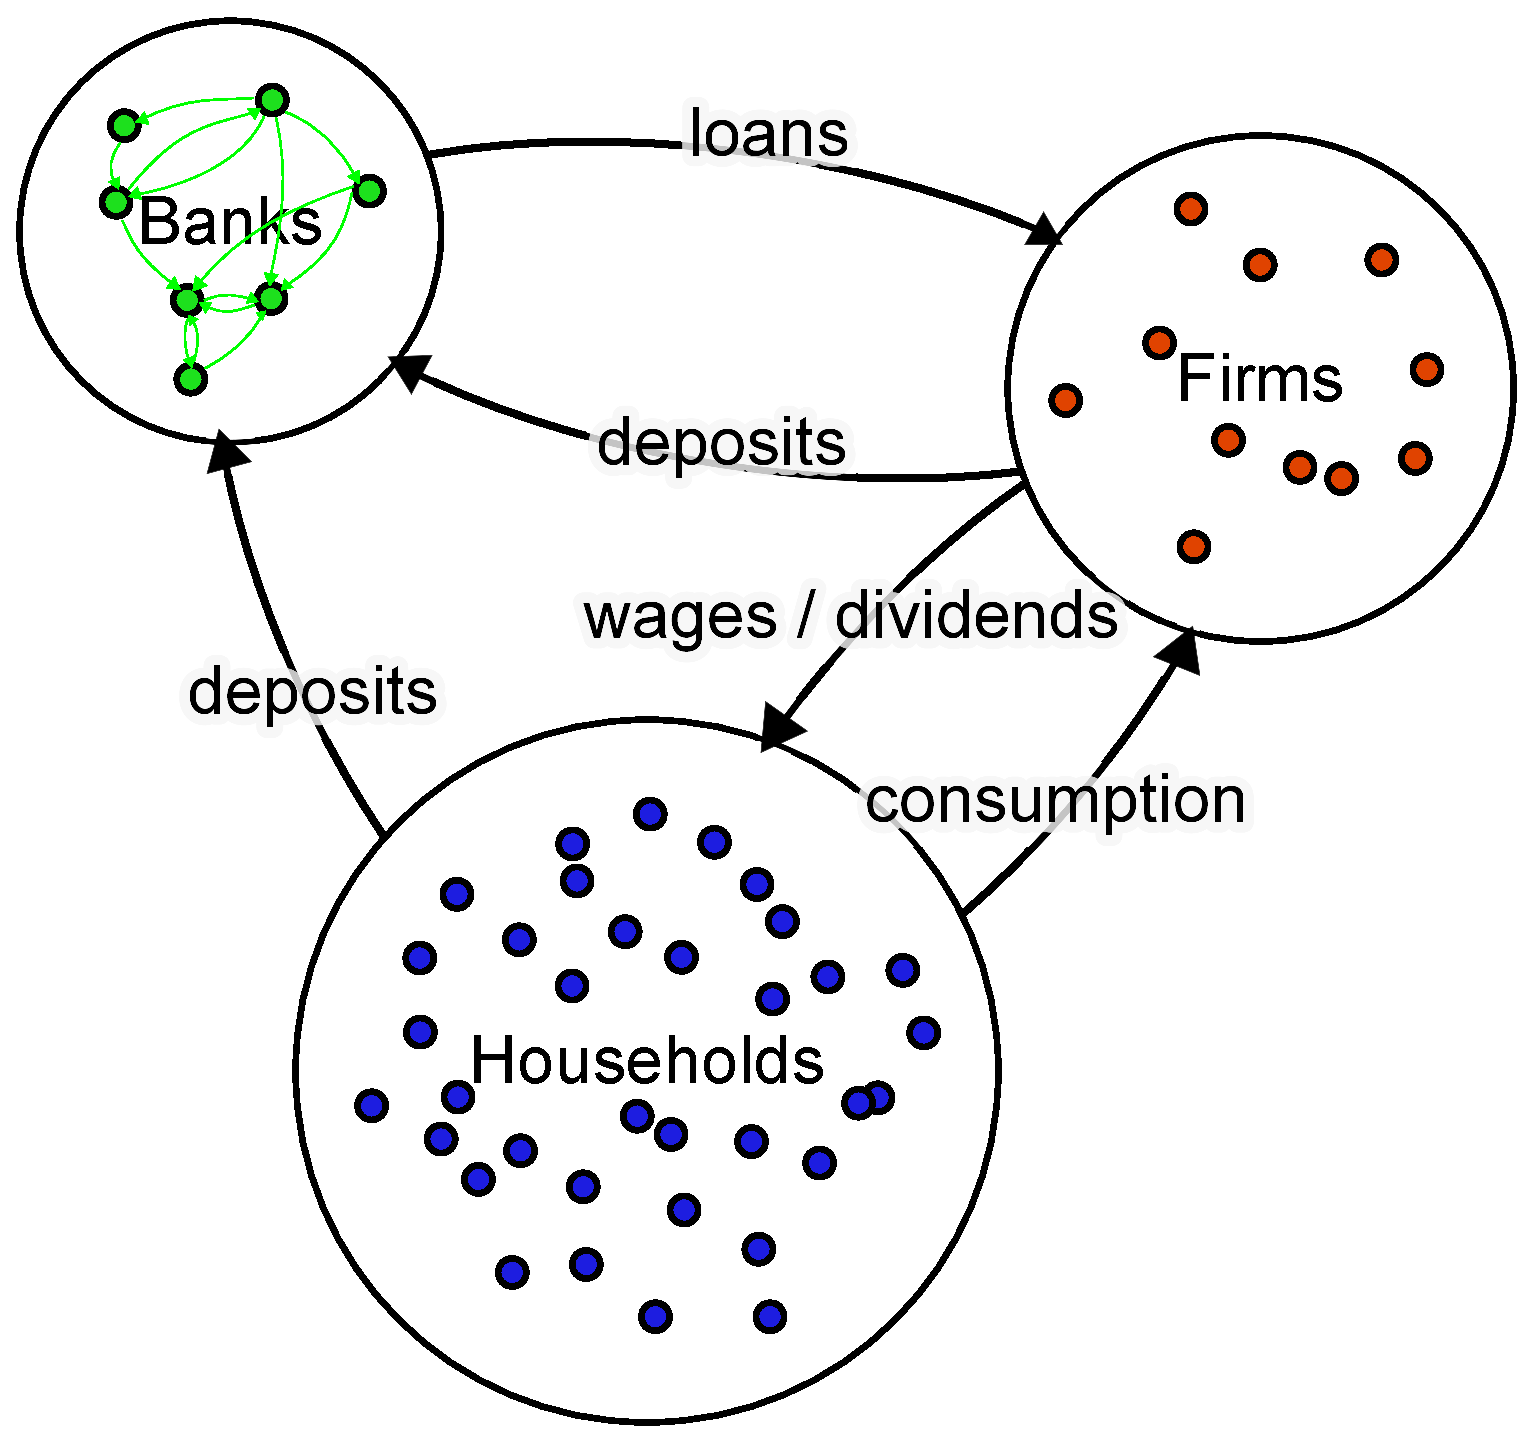
\includegraphics[width=120mm]{model}
\end{center}
 \caption{A schematic overview of the integrated model structure shows the three sets of agents -- banks, firms, and households -- and their interactions. Firms pay their owners dividends and their workers loans, the households consume goods produced by the firms. Households and firms deposit money with the banks, the banks grant loans to the firms.}
 \label{Model}
\end{figure} 

%\subsubsection{Households.}
%There are two sets of households, $I$ firm owners and $J$ workers.
%Each of them has a personal account $PA(j,t)$ at one of the $B$ banks chosen at random.
%Workers apply at $z$ different firms. 
%If hired, they receive a fixed income $w$ per time step and supply a fixed labor productivity $\alpha$.
%Firm owners receive their income as dividends from their firm's profits.
%Each household computes its consumption budget as a fixed percentage $c$ of its current personal account and spends $c PA(j,t)$ on the goods market.
%They compare the prices of goods from $z$ randomly chosen firms and buy the cheapest ones.
%
%\subsubsection{Firms.}
%There are $I$ firms producing perfectly substitutable goods with average price $\bar p(t)$. 
%Let $y_(i,t)$ be the current production stock of the company.
%Each time step they change their desired demand $d(i,t)$ and estimated price $p(i,t)$ according to the rule (or leave them unchanged otherwise)
%\begin{eqnarray}
%\textrm{ if } & y(i,t-1) = 0, \ p(i,t-1)\geq \bar p(t-1) &  \ \textrm{ then } \ d(i,t) = d(i,t-1) (1+\eta) \ \nonumber, \\
%\textrm{ if }& y(i,t-1) = 0, \ p(i,t-1)<\bar p(t-1) & \ \textrm{ then } \ p(i,t) = p(i,t-1) (1+\eta) \ \nonumber, \\
%\textrm{ if } & y(i,t-1) > 0, \ p(i,t-1)>\bar p(t-1) & \ \textrm{ then } \ p(i,t) = p(i,t-1) (1-\eta) \ \nonumber, \\
%\textrm{ if } & y(i,t-1) > 0, \ p(i,t-1)\leq\bar p(t-1) & \ \textrm{ then }\ d(i,t) = d(i,t-1) (1-\eta) \ \nonumber,
%\end{eqnarray}
%with $\eta$ being a random number drawn from $(0,0.1)$.
%Each firm computes the number of required workers to achieve the desired demand.
%If the wages for this workforce exceed the firm's current liquidity, it applies for a credit of the needed size to close the finance gap.
%Firms approach $n$ randomly chosen banks and choose the credit with the most favorable rate.
%If this rate exceeds a threshold rate $r_{max}$, the firm only asks for $\phi$ percent of the original loan volume.
%Based on the outcome of this application the firms recompute their desired workforce and hire the needed number of workers or fire their excess workforce.
%Afterwards they sell their goods on the consumption goods market.
%Firms go bankrupt if they have negative liquidity after the goods market closes.
%Each of the bankrupted firm's debtors incurs a capital loss in proportion to their investment in the company.
%Finally the firm owner immediately starts a new company with his/her personal account as equity and $d(i,t)$ and $p(i,t)$ equal to their current population average.
%
%\subsubsection{Banks.}
%Bank $b$ offers firm $i$ loans at rates $r_{bi}$ taking the individual firms' leverages into account, 
%\begin{equation}
%r_{bi} = r_{cb} (1+\epsilon) * (1+\tanh(\alpha d_i)) \quad,
%\end{equation}
%where $r_{cb}$ is the refinancing rate provided by the central bank, $d_i$ is the leverage of firm $i$, $\alpha$ a constant, and $\epsilon$ is a random number drawn from the uniform distribution between zero and one.
%Banks try to provide the loans requested by the firms and grant it if they have enough liquid resources. 
%If they do not have enough cash, they approach other banks in the interbank market and try to get the amount from them assuming zero interest rates.
%The interbank relation network is modeled as a  fully connected networks. If a bank does not have enough cash and can not raise the full amount for the requested firm-loan on the IB market, it does not pay out the loan.
%Each time step firms reimburse $\tau$ percent of their outstanding debt.
%If a bank's equity becomes negative it is insolvent and undergoes one of three possible crisis resolution procedures, (i) purchase \& assumption (P\&A), (ii) bailout, (iii) or bailin.

\section{Interbank market}\label{interbankSection}

As before banks have strategies which aim at maximising profits from capital allocation in the credit, stock and interbank market and are subject to the balance sheet identity and some regulatory constraints.  Banks set lending rates to firms and borrowing rates  to other banks in the interbank market.  Banks prefer to lend to firms and invest in the stock market, thus lending on the interbank market is residual.  

Note that the interbank lending scheme here is the one that we are planning on implementing in the integrated model, not the one that is already implemented.  In particular there are extensions to the credit market described here that allow banks to quote different interest rates to different firms, as well as different interest rates to each other.  While the ability to quote different interest rates to different firms is available in the Mark I macro model, it is not available in the other two.  We plan to implement and make the interbank lending model described here fully compatible with the rest of the integrated model at a later date.  The currently implemented interbank facility is much simpler, and only allows banks to lend and borrow at a single interest rate.

\medskip
\subsection{Definitions}
\begin{itemize}

\item $E_j(t):$ bank  equity
\item $D_j(t):$ bank deposits
\item $C_j(t):$ bank cash
\item $L_j(t):$ total bank liabilities
\item $L_j^f(t): $  total bank loans to firms
\item $L_{i,j}^f(t): $   bank $j$ loans to firm $i$
\item $I_j^l(t): $ bank total interbank lending
\item $I_j^b(t): $  bank total interbank borrowing (including from central bank)
%\item $A_j(t) = L_j^f(t) + I_j^l(t) + C_j(t):$  bank total assets
%\item $ L_j(t)=E_j(t)+D_j(t) + I_j^b(t):$ bank total liabilities 

\item  $T_f:$ maturity of loans to firms.
\item  $T_b:$ maturity of interbank loans.

\item $r_D:$ interest rate to depositors
\item $r_E:$ interest rate to banks shareholder $r_E$
\item   $r_f:$ the risk-free rate in the economy. This is the rate at which the central banks borrows from other banks
\item $r_H:$ marginal lending rate  (fixed rate at which the central bank lends to other banks)
\item  $r^f_{i,j}(t):$ interest rate offered by bank $j$ to firm $i$,  
\item  $r^l_{i,j}(t):$  interest rate asked  by bank $j$ to bank $i$,  
\item  $r^b_{i,j}(t):$ interest rate paid  by bank $j$ to bank $i$, 
\item $r^l_j(t)$ and $r^b_j(t):$ respectively the average interest rate at which bank $j$ lends and borrows in the interbank market at time $t$
\item $r^f_j(t):$  average interest rate at which bank $j$ lends to firms at time $t$
\item $p_i$ is the probability of default of firm  $i$.
\item  $\lambda_j=  \frac {A_j(t)}{E_j(t)}: $ bank leverage ratio
\item $w_{jk}(t): $ bank target level of exposure to stock $k$
\item $K_j(t): $ bank target level of exposure to private sector loans
\end{itemize}



\subsection{Sequence of Events}


At the beginning of each trading day
\begin{itemize}
 \item Banks pay interest to depositors
  \item  Banks repay their interbank loans and loans to the Central Bank
   \item Banks receive dividend payments on the stocks
    \item Banks receive interest (and principal) back on their  loans to firms (unless firm defaults)  
     \item Banks receive interest (and principal) back on their  loans to other banks  (unless bank defaults) 
      \item Banks receive interest on the cash deposited in central bank accounts 
      \item Banks pay interest to shareholder, if appropriate,  at rate $r_E$
       \item  Bank's equity is adjusted     
       \item Regulatory checks are performed and banks with negative equity are deemed to be in default 
 \end{itemize}
  After checks on banks' solvability have been performed:
\begin{itemize}
 \item Banks choose their leverage ratio $\lambda$
 \item Banks choose the weights of their asset portfolios (loans + stocks) 
\item Banks receive firms demand for loans and information about firms  probability of bankruptcy $\rho$  (firms demand is determined  in the MABM, in the tests the demand  is random and $\rho$ exogenous and the same for all firms).
\item Banks lend to firms and invest in the stock market.
\end{itemize}
After investment has taken place:
\begin{itemize}
\item Banks receive an exogenous shock on deposits (deposit fluctuations are determined  in the MABM, in the tests  the shocks are  random).
\item In case banks end up with negative positions on their central bank accounts after the shock, they enter the interbank market. If they cannot lend all they need on the IB market they borrow from the central bank at $r_H$
\end{itemize}

\subsection{Balance sheets}
 The asset side of the bank  balance sheet is  given by:
\begin{eqnarray*}
{A}_{j}(t) &=& C_{j}(t) + \mathbf{s}_{j,t}^T \mathbf{p}(t) + \sum_{i=1}^{N_f} L^f_{j,i}(t) + \sum_{i=1}^{N_b} I^l_{j,i}(t), \\
\mathbf{s}_{j}(t) &=& \left(s_{j1}(t),...,s_{jN_f}(t) \right)^T,\\
\mathbf{p}({t}) &=& \left(p_{1}(t),...,p_{N_f}(t) \right)^T,
\end{eqnarray*}
where $C_{j}(t)$ is the cash investment, $\mathbf{s}_{j}(t)$ the vector of stock ownership, $\mathbf{p}(t)$ the vector of share prices, $N_f$ is the number of shares and $L_{j,i}(t)$ is the book value at time $t$ of a loan extended from bank  $j$ to firm $i$, and $I^l_{j,i}(t)$ is the book value at time $t$ of a loan extended from bank  $j$ to bank $i$.
Intermediaries face a long only constraint, i.e. $s_{j,i}(t) \geq 0$. This implies that intermediaries cannot short an asset which they consider overpriced. This limits the extent of arbitrage that is possible in this setting. Mispricings may therefore be able to persists longer than in the case of permitted short selling.
\\\\
The liability side of the bank  balance sheet is  given by:
\begin{equation*}
{L}_{j}(t) = D_{j}(t) +  \sum_{i=1}^{N_b} I^b_{j,i}(t), \\
\end{equation*}
where $D_{j}(t)$ is the size  of deposits of bank $j$, and $I^b_{j,i}(t)$ is the book value at time $t$ of a loan extended from bank  $i$ to bank $j$.
By definition the equity of the intermediary is given by:
\begin{equation*}
{E}_{j}(t) ={A}_{j}(t) -{L}_{j}(t),
\end{equation*}
where ${L}_{j}(t)$ generically represents all liabilities of intermediary $j$ at time $t$. We assume, for simplicity, that the intermediaries do not face funding restrictions, i.e. should the intermediary decide to increase its liabilities it always finds willing lenders.

\subsection{Beginning of day regulatory check}
At the beginning of the trading day banks pay interest to depositors,  repay their interbank loans and loans to the Central Bank, receive dividend payments on the stocks, receive interest (and principal) back on their  loans to firms (unless firm defaults),  receive interest (and principal) back on their  loans to other banks  (unless bank defaults), receive interest on the cash deposited in central bank accounts. Bank's equity is adjusted as follows 

\begin{equation*}
{E}_{j}(t) = {E}_{j}(t-1) +  d{E}_{j}(t)
\end{equation*}
where 
$$
d{E}_{j}(t) = C_{j}(t-1) r_f +  \sum_{k=1}^{N_f} s_{j,k}(t-1){d_k}(t)+ 
\sum_{i=1}^{N_f} L^f_{j,i}(t) r^f _{j,i}(t-1)+
$$$$
 \sum_{i=1}^{N_b} I^l_{j,i}(t) r^l _{j,i}(t-1) -  \sum_{i=1}^{N_b} I^b_{j,i}(t)  r^l _{j,i}(t-1)-  D_{j}(t-1) r_D.  \\
$$
If Bank equity is negative at this point the bank goes into default. 

\subsection{Credit Market}

We present here a possible model for the credit market that allows for cross-sectional interest rate dispersion in both the loans and interbank market.  The model allows for a predetermined connectivity network between firms and banks and in the interbank market. The modelling choice for the interbank credit market mimics the behaviour of the e-Mid interbank market  which is a transparent trading platform.   Alternative mechanisms, based on over the counter trading  (OTC)  are of course  possible.  


\subsection{Lending to firms}

 Once banks have determined the proportion of loans in their portfolio $w_{j,L}$ they submit loan offers to firms for a total of $\hat L^f_j(t) = w_{j,L} \lambda_j E_j(t)$. 
 Banks take into account the  their financing costs and the firm probability of default when determining their lending rates (the probability of firm default  is an input from the MABM). 
 We assume here that firms are equally risky  (extension to heterogenous firms will be consider at a later stage). The  bank to firm rate is  bounded from below by  the interest rate to depositors (that we assume to be higher  than  the risk-free rate). Additionally the reservation (lowest)  price  at which bank $j$  is willing to lend to firm $i$ take into account the risk of firm default and   is  
determined  by the condition
\begin{equation}
(1+r^{min}{ij}(t))(1-p_i) +  \gamma p_i=(1+ E[r^b_{j}(t)])  > (1+r_f) \quad \forall j,
\end{equation}
or
\begin{equation}
r^{min}_{ij}(t)= \frac{1+E[r^b_{j}(t)] -\gamma p_i}{1-p_i}  -1 ,
\end{equation}
 where $p_i$ is the probability of default of firm $i$,  $\gamma$ is  the recovery rate in case of firm default  (we currently  assume that  $\gamma=0$,   in Basel $\gamma=45\%$). 
 
 $E[r^b_{j}(t)]$ is the rate at which  bank $j$ expects to borrow in the interbank market at day $t$. $E[r^b_{j}(t)]$  calculated as a volume weighted average of past rates obtained in the interbank market 
 \begin{equation}
E[r^b_j(t)]= {\sum_{\tau= 1}^n   r^b_j(t- \tau) \frac{I^b_j(t-\tau)}{\sum_{\tau= 1}^n {I^b_j(t-\tau)}}}.
\end{equation}
This rule reflects the assumption  that the bank lends to firms at least at the rate it expects to borrow in the interbank market in case of a  negative liquidity shock.  The  expected rate incorporates the liquidity risk.
In the above equation, if the bank has not borrowed in one of the previous period we set  $r^b_j(t- \tau)=0$ in the sum.  If a bank receives shocks that are small compared to the exposure level, so that the bank does not need to borrow in the interbank market, it can afford to  set lower rates to firms. As a result (the precise mechanism is explained later), such bank will also try and  increase  its leverage target $\lambda_j$.  Vice versa a bank that has large deposit fluctuations given its level of chosen leverage, has to charge higher rates to firms.  Eventually bank learn to choose  $\lambda_j$ compatibly with the volatility of their deposits. 

We assume that firms are price takers but have a stepwise demand function and do not accept rates higher that $r_{max}$ (linked to the CB policy rate).
 Note that the bank may not achieve the desired level of  lending to firms (for example if $w_{j,L}$ is too high or the rates offered to firms are too high). $L^f_j(t)$ represents the actual amount of loans to firms provided by banks $j$ at time $t$.
 
  Firms approach first banks (possibly only a subset to which the are connected) that offer them  the best rate.   Banks lending  to firms occurs on a first come first served basis.


\subsection{Shocks to deposits}
After banks have committed to  lend to firms and invest in the stock market, a shock, $dD_j(t)$, on banks' deposit  occurs (this is determined by the macro model, though for testing purposes we replace this by exogenous shocks).

In case the shock on deposit on bank $j$  is such that $D_j((t) >  C_j((t)$  then bank $j$ enters the interbank market and requests an interbank  loan of size
\begin{equation}
I^b_j((t)= dD_j(t) - C_j((t) 
\end{equation}

  On the contrary, if the shock  on deposits  is positive, or if  it is sufficiently small that the bank is left with cash reserves, $C_j(t)>0$, the bank will try and   lend $C_j(t)$ in the interbank market.


\subsection{The interbank market}
 Given the amount of loans committed by banks to firms and the bank equity  (information as we mentioned is public)  the probability of defaults of each banks can calculated  from the probably of defaults of loans to firms (i.e. probability that losses on firm lending exceed equity). Currently we use a normal approximation to the binomial distribution of losses which assumes each loan is the same size, has the same probability of default,  and the defaults are  independent.
 
In the case of correlated defaults, we plan to use the one factor Vasicek model used to calculate the Internal Ratings-Based (IRB) approach of Basel II. To this purpose we assume that banks  make loans that are all the same in size and to firms who have the same  probability of default. Denote by $p^f$  the (time independent) fraction of loans to banks that may default.
The cumulative distribution of the random variable $p^f$   under the Vasicek model is
\begin{equation}
F(p^f) = N \left( \frac{\sqrt{1-\rho} N^{-1}(p^f) -  N^{-1}( p)}{\sqrt {\rho} }\right )
\label{conditional}
\end{equation}
 where $p$ is the unconditional probability of each loan (or firm) defaulting (we assume $p_i=p$ for all firms) and $\rho$ is the loans exposure to the systematic risk factor in the Vasicek model.
 
 Thus the probability of a bank $i$ default is
\begin{equation}
p_i^b=P\left( p^f  \geq  \frac{E_j(t)}{L_j(t) }\right) = 1- N \left( \frac{\sqrt{1-\rho} N^{-1}\left( \frac{E_j(t)}{L_j(t) }\right) -  N^{-1}(p_i)}{\sqrt {\rho} }\right )
\label{DefaultProbability}
\end{equation}

The assumption in the model is that the probability of default of each bank is common knowledge in the market. The implicit assumption is that a credit rating agency provides this information to the market, or CDS spreads are available for any potential counterpart. Various weakened and more realistic versions could be considered. For example banks may know other banks probability of default with some uncertainty, or may be looking at the historical probability of defaults. 

Once the shock to deposits has been realised, lending on the interbank market does not bear liquidity risk and  banks are willing to lend  all their excess cash, as long as they can make an expected  profit (accounting for the risk of default of borrowers) at least comparable to leave money in central banks deposits. This is  a strong assumption that limit the possibility of strategic liquid it hoarding of liquidity. In the future we can generalise to deposit shocks and demand for loans  happening at random times during the day so that banks have to take their interbank lending  decision while facing this uncertainty. Initially, for simplicity,  interbank lending is left until the end of the business day. 

Lenders reservation prices are determined by the conditions 
 \begin{equation}
(1+r^l_{i,j}((t))(1-p^b_i) + \gamma p^b_i=(1+r_f) \quad \forall i,j,
 \end{equation}
Lender $i$  accepts any offer from a borrower $j$ as long as its reservation rice is lower that the rate offered by the borrower:
 \begin{equation}
r^l_{i,j}((t)= \frac{(1+r_f - \gamma p^b_j)}{1-p^b_j }- 1 <  r^b_{j}((t))
 \end{equation}
%Each lender $i$ charges an additional  spread to the reservation price trying to maximising profits so that the rate bank $i$  is willing to accept from bank $j$ is 
% \begin{equation}
% r^l_{i,j}(t)  =\frac{(1+r_f - \gamma p^b_j)}{1-p^b_j } -1 + \Delta r_i(t)
% \label{interbank rate}
%  \end{equation}
  
  Borrowers  compete for liquidity  and they post bids at the rate 
   \begin{equation}
 r^b_{j}(t)  =\frac{(1+r_f - \gamma p^b_j)}{1-p^b_j } -1 + \Delta r_j((t)
 \label{interbank rate}
  \end{equation}

Borrowers try and learn which is the lowest  spread they can  offer in order  to satisfy their demand  for loans. 
 
 
We assume that lending is restricted to an exogenous pre-determined network (to model market frictions). This is currently done via a fixed (for each simulation) Erdos-Reyni random graph. This allows us to go from the extreme of an anonymous fully connected market (i.e. $p = 1$) to a very weakly connected market.


Borrowers post their bids and lenders, in random order: observe their neighbours borrowers bids, compute the profitability of each bid as
  \begin{equation}
\pi_{i,j}(t) = [ r^b_{j}(t) - r^l_{i,j}(t)] = \Delta r_j(t),
\end{equation}
 rank them and fill them in order of profitability. 
 
\subsection{Learning}
\label{learning}
\subsection*{Bank rates to firms}
The lending rate to firm is updated so to try and achieve the target level $\hat L^f_j(t)$.
 If the bank has not been able to lend all the desired level to firms it reduces the rate following the rule
 \begin{equation}
r^f_{i,j}(t) =\min \left\{ r^{max}, \max \left\{r_D, r^{min}_{i,j}(t-1),  r^f_{i,j}(t-1)
\left[1 + \epsilon^f \frac{L^f_j(t-1) - \hat L_{j}(t-1)}{\hat L_{j}(t-1)}\right] \right\} \right\}
\end{equation}
where $\epsilon_r>0$.
 If the bank has  been able to lend all the desired level to firms, with probability $p$  it increases  the rate to 
 \begin{equation}
r^f_{i,j}(t) =\min \left\{ r^{max},  r^f_{i,j}(t-1) \left[1 + \epsilon^f \right] \right\} 
\end{equation}


  \subsection{Interbank market spreads}
  Spreads on interbank market are updated following a similar rule as to bank rates to firms.
%   Lenders calculate how much they have managed to lend in the previous period, $\tilde I^l_j(t-1)$ and compare it to their available liquidity $I^l_j(t-1)$and adjust the rate as follows
% \begin{equation}
%\Delta r^l_{j}(t) = r^l_{j}(t-1)\left[1 - \epsilon_r \frac{I^l_j(t-1) -\tilde I^l_j(t-1)}{I^l_j(t-1)}\right] 
%\end{equation}
Borrowers  calculate how much they have managed to borrow in the previous period (without recurring to CB),
 $\tilde I^b_j(t-1)$ and compare it to their  liquidity demand  $I^b_j(t-1)$ and adjust the rate as follows
 
 \begin{equation}
\Delta r^b_{j}(t) = \Delta  r^b_{j}(t-1)\left[1 + \epsilon^b  \frac{I^b_j(t-1) -\tilde I^b_j(t-1)}{I^b_j(t-1)}\right] 
\end{equation}
If the bank has  been able to borrow all the desired liquidity, with probability $p$  it decreases  its interbank borrowing rate   to 
 \begin{equation}
\Delta r^b_{j}(t) = \max \left\{ 0, \Delta r^b_{j}(t-1) \left[1 - \epsilon^b \right] \right\} 
\end{equation}

\subsection{Bank leverage target}
 After $P$ steps the banks  revise their leverage target in the following way. Different updating strategies are possible. 
 Here we illustrate a possible one. They calculate the average  profit over the  $P/2$ previous steps (to allow time to learn the rate) as follow:
  
$$
 \Pi (\lambda_j) =  {2\over P} \sum_{\tau =1}^{P/2} [ \sum_{k =1}^{N_f}s_{j,k}(t-\tau)r_k(t-\tau) +
 \sum_{k =1}^{N_f}L^f_{j,i}(t-\tau) *r^f_{j,i}( t-\tau) -
 $$$$
 \sum_{k =1}^{N_b}I^l_{j,i}(t-\tau) *r^l_{j,i}( t-\tau) 
 - \sum_{k =1}^{N_b}I^b_{j,i}(t-\tau) *r^b_{j,i}( t-\tau)  ]
$$
Each banks they select a new value for $\lambda_j$ (from a  discrete possible set of values) with probability 
  \begin{equation}
p(\lambda_j) = \frac{e^{\beta \Pi(\lambda_j)}}{\sum_i e^{\beta \Pi(\lambda_i)}}
  \end{equation}
  This rule may possibly lead to unrealistic large strategy jumps which we may control by adding  an inertia term.

Overall the strategy optimisation is against fixed historical data, and does
not incorporate any strategic consideration regarding how other banks would react. Further development in this direction will be considered.

\bibliography{Refs,crisis_82} 
\bibliographystyle{chicago}

\newpage
\chapter{Planned Future Direction}\label{Chapter2}
\tikz[remember picture,overlay]
\node[rotate=0,opacity=0.15,inner sep=0pt,right=1cm,above=-12cm] at (current page.center){\includegraphics[scale=1.0]{./CRISIS-full.big.png}};
\clearpage
\newpage

\section{Introduction}
In this document we outline a draft proposal for the development of the CRISIS framework stimulated by our meetings and discussions with the Bank of England. It incorporates inputs from the following internal CRISIS documents:
\begin{itemize}
  \item Strawman Specs (Ross, Milan, Olaf, Doyne) \cite{Richardson14a}
  \item Specification for CRISIS Development (Ross, Doyne) \cite{Richardson14b}
  \item BoE Action Plan (Christoph, David, Doyne) \cite{Aymanns14}
  \item Shadow banking proposal (Gerald) \cite{Gurtner14}
  \item Bank strategy proposal (Christoph) \cite{Aymanns14a}
  \item Proposal for securitized lending to households (David, Olaf) \cite{Pugh14}
  \item Integration Report.
\end{itemize}
The primary goal of these changes is to allow our model to capture a more complete and accurate description of the (UK) economy based on the feedback we got on the current model (see \cite{Burrows14}).

\subsection{Summary of Proposed Changes}

In the following we organize changes into three categories, corresponding to which of the three basic types of agents are most affected: households, firms, and financial agents (i.e. banks, funds and shadow banks). There are also structural changes corresponding to heterogeneity in risk and timescales.  Figure~\ref{fig:plumodel} illustrates the money flows and interactions in the new scheme. 

\begin{enumerate}
\item
\textbf{\textit{Changes primarily affecting households}}.
\begin{enumerate}
\item
{\it Housing market}.  We  introduce home ownership so that the household decision involves how much to save, consume, or spend on housing.  Banks lend to households to allow them to purchase housing.
\item
{\it Ownership of the economy}.  Households will be the ultimate owners of both firms and banks.  This ownership is mediated through funds.  Households split their savings between bank deposits and mutual funds.  Each household is initially randomly matched to a fund, but afterward can change funds based on performance.  Dividends and loan payments are passed back automatically through the mutual funds to the households owning their shares. Households can redeem their mutual fund investments to meet their consumption needs.
\item
{\it Life cycle}.  We will allow for the possibility that households have ages.  Households can die and new households are injected, and decision making may depend on the age of the household.
\end{enumerate}
\item

\textbf{\textit{Changes primarily affecting the financial sector}}
\begin{enumerate}
\item
{\it Stock trading} will be primarily done by funds.  It can also be done by banks, but we will be able to control the fraction of stocks held in a bank's portfolio, including the possibility that the fraction is zero.
\item
{\it Mutual funds} trade shares in stocks and also issue loans (which should be thought of as bonds) to banks.  Each household will be associated with a mutual fund; households put their savings into mutual funds and can remove them if they need them, e.g. to buy a house.
\item
{\it Pension funds}
\item
{\it Banks borrow} from funds.  This is modeled as a bond.  New bonds can be issued and existing bonds can be sold. 
\item
{\it Risk weighted capital constraints} as done in Basel III will be introduced in order to make risk management more realistic.
\item
{\it Banks' portfolio allocation decisions} will be handled via an improved algorithm.
\item
{\it Liquidity constraints} will be introduced as well as the current solvency constraints.
\item
{\it Interbank market}.  A project has been underway for some time to add an interbank market.  That should reach completion soon.  Interbank trading will focus on overnight lending and interactions with the central bank.
\item
{\it Secondary market for loans}.  One of the open issues we have struggled with is whether to implement a secondary market for loans.  The argument against this is that it involves pricing loans with a continuous range of maturities and variable risks; the arguments in favor are that otherwise both funds and banks may be constrained from liquidating their assets.  This is particularly problematic for banks as it makes it very difficult for them to deleverage (and we may miss important contagion effects if we cannot do this).  We are deferring a decision on this point while seeking more advice.
\end{enumerate}
\item
\textbf{\textit{Changes primarily affecting firms}}.\\
The decision making rules for firms will act over a longer horizon and will change more slowly, corresponding to longer period optimization.
\item
\textbf{\textit{Heterogeneity}}
\begin{enumerate}
\item
{\it Heterogeneous risks}.  We will allow both firms and banks idiosyncratic risks yielding heterogenous interest rates.
\item
{\it Heterogenous timescales}.  We will create {\it realistic timescales for contracts}, both in terms of their maturity and repayment schemes.  We will do this by matching the profile of loans actually given, with the goal of obtaining an accurate representation of {\it maturity transformation}. Furthermore, the horizons of agents' decision-making will be adjusted based on the typical timescales for agents to act.
\item
{\it Heterogeneous market clearing}.  We will use a method developed by our collaborator Gerald Gurtner \cite{Gurtner14} as way to achieve heterogenous interest rate pricing, and clear the bond market and the stock market simultaneously once a day.
\end{enumerate}
\item
\textbf{\textit{Scale and the use of heterogeneous representative agents}}.\\
Due to computational limitations agents will be modeled on different scales with varying degrees of heterogeneity.  In particular:
\begin{enumerate}
\item
{\it Financial agents}. Given that there are less than 20 important banks in the UK and the number of funds is relatively small, we should be able to model them at one-to-one scale.
\item
{\it Households}.  There are roughly 20 million households in the UK and so it is computationally infeasible to model them all.  Since the number of households we can reasonably simulate is in the range of $1,000 - 10,000$, we will therefore plan on having each simulated household represent $2,000 - 20,000$ real households.  These households will be heterogeneous, in that they will correspond to households with different wealth, income and age (and in the future possibly other variables).
\item
{\it Firms}.  There are the order of three million firms in the UK.  However most of these are small, so we propose to model a few hundred of the largest firms on one-to-one scale and then model the remaining firms in terms of representative agents.  The precise breakdown remains to be determined after gathering more data.   The number of firms must also be chosen in concert with the number of goods as in some cases we want to allow multiple firms per good.
\end{enumerate}
\end{enumerate}

Figure~\ref{fig:plumodel} illustrates the money flows and interactions in the new scheme. 
\begin{figure} %[b]
\caption{The basic elements of CRISIS 3.0.  Arrows illustrate the direction of money flow in the new scheme to pay for goods, services and financial assets. For contracts such as bonds, where money initially flows in one direction and then returns, the arrow indicates the initial flow of money.  The dashed arrow indicates an optional flow that can be switched on and off.}
\centering
\includegraphics[scale=0.6]{CRISIS-full.png}
\label{fig:plumodel}
\end{figure}

\subsection{Plumbing vs. decisions}

When reading this document it is sometimes useful to distinguish \emph{Plumbing} vs. \emph{Decisions}:

\textbf{\emph{Plumbing}} refers to features of the framework that are primarily structural and do not depend on behavioral assumptions.  The plumbing is intended to relatively static and not expected to change significantly over timescales of six months to a year.  Examples include the introduction of new markets, new types of agents and new types of contracts that can be held on the balance sheets. Plumbing also encompasses necessary changes to introduce heterogeneous timescales into the framework. For example, we want contracts such as bonds to have multiple maturities and variable repayment schemes. 

\textbf{\emph{Decisions}} on the other hand are encapsulated plug-ins allowing us to specify and vary the behaviour of agents in the model. This includes the behavioural rules of agents and typical timing of their decisions. Such changes are often experimental, and determining the most appropriate decision rules typically involves open research questions, and we plan to be changing these on a regular basis.  The decision rules given here should we regarded as default examples, which at this stage are just plausible choices to allow us to make simulations and test the models.  Refinement of the decision rules will be one of the main activities during the remainder of the project.

While we do not spell these out, the difference should be clear and it is useful to bear in mind that the decision rules are in general quite malleable.

We now give further details on the proposed changes.


\section{Changes primarily affecting households \label{householdModel}}

There are roughly 20 million households in the UK and it is computationally infeasible to model them all.  Since the number of households we can reasonably simulate is in the range of $1,000 - 10,000$ each simulated household represents $2,000 - 20,000$ real households.  Note that each of the households in our model are heterogeneous in that, at a minimum, have different levels of wealth and income.\footnote{Households will also likely have different behavioral parameters.}

In previous versions of the CRISIS model household behavior was incredibly simple: each household devoted a constant fraction of its wealth to consumption expenditures and saved the remaining fraction as bank deposits. The most recent version of the CRISIS extends the household behavior along a number of dimensions.

In addition to bank deposits, households now have access to two additional savings vehicles: housing and mutual funds. In most developed countries a house is the most valuable asset of the majority of households. Empirically, secured lending to households accounts for between 2/3 and 3/4 of all bank lending in the UK. While households are the ultimate owners of both firms and banks, this ownership is mediated through mutual funds. Our primary justification for including mutual funds is institutional realism: households commonly own shares in firms and banks indirectly via mututal funds and mututal funds are an important source of medium to long term financing for banks.
%Secured lending against either commercial or residential real estate accounts for around two-thirds of all bank lending in the UK \cite{Burrows14, Turner14}. In \cite{Pugh14} we introduce a stylised residential housing model into the CRISIS framework. Our approach builds on previous work by \cite{kiyotaki1997credit} and \cite{iacoviello2005house}.

In what follows, we sketch a basic framework for introducing mutual funds as well as secured lending to households. Our model of secured lending is inspired by \cite{hart1994theory,iacoviello2005house,kiyotaki1997credit}.\footnote{
%
The gory details of the model are discussed in \cite{Pugh14}.}
%
The primary research focus of our stylised model is on the role of loan-to-value (LTV) and income-to-value (ITV) constraints in generating housing price cycles in a model with substantial household heterogeneity. Thoughout we assume a fixed supply of housing and a fixed population of households.\footnote{
%
An extended version of our model will incorporate a construction sector which will allow for variable housing supply and population. Our extended model will allow us to study credit refinancing cycles and first time home owner transitions induced by age dependent consumption and generation-driven turnover of assets.}
%

\subsection{Household preferences}

We begin by supposing that household $i$ wishes to choose levels of borrowing, $b_{i,t}$, deposits, $d_{i,t}$, aggregate non-durable consumption, $C_{i,t}$, housing, $h_{i,t}$, and mutual funds, $m_{i,t}$ in order to maximize
\begin{equation}
    V_t = E_t\left\{\sum_{s=0}^{\infty} \beta_i^s \min \left(\omega_i C_{i,t+s}, (1-\omega_i) h_{i,t+s}\right)\right\}
\end{equation}
where $0 < \omega_i < 1$ is a utility weight for consumption relative to ownership of housing stock, and $0 < \beta_i < 1$ is the household discount factor and the expecations operator $E_t$ is a subjective expectations operator.\footnote{
%
The upshot of our assumption that aggregate consumption goods and housing are perfect complements is that households will prefer to hold consumption goods and housing in fixed proportions.  Recall that CRISIS households have Dixit-Stiglitz preferences over individual consumption goods and that the decision of how best to allocate resources across the various consumption goods can be treated separately from the housing decision discussed here.
\begin{equation}
  C_i(h_t) = \left(\frac{1-\omega_i}{\omega_i}\right)h_{i,t} \notag
\end{equation}} 
%
Motivated by empirical work by John Muellbauer, we assume that household expectations of future variables are formed using either adaptive or extrapolative rules. Our households do not have rational expectations. 

Note that our approach to housing assumes that housing is a fluid good, so that a given``household'' can purchase a little more or sell a little housing at any given point in time.  To understand why this makes sense recall that our households actually represent a bin with thousands of individual households who have similar values of income, wealth and possibly other characteristics (such as age).  Thus we expect that at any given time a few houses may be buying or selling, and the overall amount of ``housing'' contained in the bin may change incrementally on a day by day basis.

\subsection{Household constraints}

Household $i$ faces a number of constraints that substantially restricts the levels of borrowing (i.e., mortgage debt), deposits, and housing that it can acquire. Consider the balance sheet of household $i$ at the start of date $t$.
\begin{table}[h]
    \begin{center}
    \begin{tabular}[H]{ c | c }
         Assets & Liabilities  \\
        \hline
         $q_{h,t} h_{i,t-1}$ & $R_{t-1}b_{i, t-1}$ \\
         & \\
         $q_{m,t} m_{i,t-1}$ & \\
         & \\
         $R_{f, t-1}d_{i,t-1}$ & Equity\\
    \end{tabular}
    \end{center}
\end{table}
From the household balance sheet we have three sources of funds: housing wealth, $q_{h,t} h_{i,t-1}$, mutual fund wealth, $q_{m,t}m_{i,t-1}$, and bank deposits, $R_{f, t-1}d_{i,t-1}$. Household $i$ also has two additional sources of funds: its nominal income $y_{i,t}$, and new borrowing $b_{i,t}$. Together total household available resources (i.e., ``sources'' of funds) are as follows.\footnote{
%
The way that I have currently specified the decision problem assumes that mutual fund shares, $m_{i,t}$, is a choice variable for the household. An alternative specification would to assume that the quantity of mutual fund shares is effectively fixed in which case total household resources are
\begin{equation}
  y_{i,t} + q_{h,t} h_{i,t-1} + \Pi_{i,t} + R_{f, t-1}d_{i,t-1} + b_{i,t} \notag
\end{equation} 
where $\Pi_{i,t}$ represents the value of mutual funds shares owned by household $i$.}
%

\begin{equation}
  y_{i,t} + q_{h,t} h_{i,t-1} + q_{m,t} m_{i,t-1} + R_{f, t-1}d_{i,t-1} + b_{i,t}
\end{equation} 

Total household expenditures consist of new housing purchases $q_{h,t} h_{i,t}$, repayment of accumulated debt of $R_{t-1}b_{i, t-1}$, the purchase of consumption goods, $P_t C_{i,t}$, the purchase of additional mutual fund shares, $q_{m,t}m_{i,t}$, and any desired residual deposits $d_{i,t}$. The following summarizes total household expenditures (i.e., ``uses'' of funds).
\begin{equation}
  P_t C_{i,t} + q_{h,t} h_{i,t} + q_{m,t}m_{i,t} + R_{t-1}b_{i,t-1} + d_{i,t}
\end{equation}

A household's flow-of-funds constraint simply requires that total household expenditures in a given period equal a household's total available resources. 
\begin{align}
    \text{Uses} \equiv &P_t C_{i,t} + q_{h,t} h_{i,t} + q_{m,t}m_{i,t} + R_{t-1}b_{i,t-1} + d_{i,t} =\notag\\ &y_{i,t} + q_{h,t} h_{i,t-1} + q_{m,t} m_{i,t-1} + R_{f, t-1}d_{i,t-1} + b_{i,t} \equiv \text{Sources}
\end{align}

In addition to the flow of funds constraint, we assume that household $i$ faces both loan-to-value (LTV) and income-to-value (ITV) constraints which further restrict its borrowing and housing purchases.\footnote{
%
Empirical relevance of both LTV and ITV constraints is documented by the BoE data from Katy's talk. Need more formal citation. }
%In addition to the empirical justification, there are a number of theoretical justifications for LTV constraints.  For example \cite{hart1994theory} argue that households can not borrow against future labour income because it is not possible to credibly pre-commit to work in the future. This in ability to pre-commit means that borrowers must post seizable collateral in order to borrow. Currently we do not know whether or not there is some microeconomic justification for an LTV constaint such a constraint independent of the LTV constraint.
%
We implement an LTV constraint similar to the one used by \cite{kiyotaki1997credit} and \cite{iacoviello2005house}. Specifically, we assume that a bank will take care to insure that the total value of the loan (i.e., principle and interest) to household $i$ is less than some fraction of the market value of its stock of durable housing at end of date $t$. Note that our formulation allows the asset being purchased to function as the collateral for the loan.
\begin{equation}
    R_t b_{i,t} \le (1 - \theta_{i,t}) q_t h_{i,t}
\end{equation}
The parameter $0 < \theta_{i,t} < 1$ denotes the `haircut'' which in principle can vary across both households and time. Similarly, our implementation of the income-to-value (ITV) constraint assumes that the lender will take care to insure that the value of housing purchased by household $i$ does not exceed some multiple $\mu_{i,t} > 1$ of its income.
\begin{equation}
    q_t h_{i,t} \le \mu_{i,t} y_{i,t}
\end{equation}
The ability to analyze the endogenous interaction between the LTV and ITV constraints in a model with substantial household heterogeneity is a key feature of our model.

An additional feature of housing stock, one that differentiates it from deposits and mutual funds, is that housing stock is a relatively illiquid asset. Whilst a household can always demand its deposits and sell shares in mutual funds it is decidedly more difficult to sell a house. To capture the relative illiquidity of money we follow \cite{kiyotaki2012liquidity} and make a reduced form assumption that a household can only sell a fraction $0 < \phi < 1$ of its housing stock in any given period. 
\begin{equation}
    h_{i,t} \ge \phi h_{i,t-1}
\end{equation}
 We assume that $\phi$ is a constant. The overall liquidity of the housing market does not vary across time or households.

Finally, we assume that household $i$ faces non-negativity constraints on borrowing (i.e. we do not allow households to lend) and mutual fund holdings (i.e., we do not all households to short mutual funds); and positive lower bounds on both deposits and housing stock. Note that the assumed lower bound on housing stock implies a lower bound on consumption as well.
\begin{align}
  b_{i,t} \ge& 0 \\
  C_{i,t} \ge& \left(\frac{1-\omega_1}{\omega_i}\right)\underline{h} \\
  d_{i,t} \ge& \underline{d} \\  
  h_{i,t} \ge& \underline{h}
\end{align}

\subsection{Household decision rules}
Our model of household, though stylised, is capable of generating rich behavioral dynamics. Key state variables for households in our model are income and net worth (i.e., equity). In this section, in order to give some intuition on the type of behavioral rules being used by households in the model, we discuss four behavioral regimes that the Bank of England mentioned as being particularly relevant given their data: loan-to-value (LTV) constrained household, income-to-value (ITV) constrained households, renters, and cash-buyers.\footnote{In general, households will coexist in each of these behavioral regimes simultaneously.} 

\subsubsection{Loan-to-value (LTV) constrained households}
Loan-to-value (LTV) constrained households are leveraged home-owners. In fact, LTV constrained households are sufficiently leveraged that they will have upward sloping demand curves for housing!\footnote{In her presentation, Katy specifically mentioned that they can observe these upward sloping demand curves in the data.} With upward sloping demand curves, LTV constrained households will want to expand their holdings of housing as much as possible meaning that they will choose to run down their deposit and mutual fund accounts. 

Formally, LTV constrained households use the following decision rules for choosing borrowing, consumption, deposits, housing, mutual fund holdings:
\begin{align}
    b_i(n_{i,t-1}, y_{i,t}) =&\left(\frac{1-\theta_{i,t}}{R_t}\right)q_{h,t} h_{i}(n_{i,t-1}, y_{i,t}) \\
    C_i(n_{i,t-1}, y_{i,t}) =& \left(\frac{1-\omega_i}{\omega_i}\right) h_{i}(n_{i,t-1}, y_{i,t}) \\
    d_i(n_{i,t-1}, y_{i,t})=& \underline{d} \\
    h_i(n_{i,t-1}, y_{i,t}) =& \left(\frac{1}{P_t \left(\frac{1-\omega_i}{\omega_i}\right) + \left(\frac{(R_t - 1) + \theta_{i,t}}{R_t}\right)q_{h,t}}\right)\bigg[y_{i,t} + n_{i,t-1} - \underline{d}\bigg] \\
    m_i(n_{i,t-1}, y_{i,t}) =& 0
 \end{align}
where $n_{i,t-1}$ denotes the net worth (i.e, equity) of household $i$.
\begin{equation}
  n_{i,t-1} = q_{h,t} h_{i,t-1} + R_{f,t-1}d_{i,t-1} + q_{m,t}m_{i,t-1} - R_{t-1}b_{i,t-1}
\end{equation}

\subsubsection{ITV constrained households}
Income-to-value (LTV) constrained households are also leveraged home-owners. However, unlike LTV constrained households, ITV constrained households do not have upward sloping demand curves for housing.\footnote{Again, Katy's presentation said that they can observe ITV constrained households in the data and that the data support a textbook downward sloping demand curve.} 

Formally, ITV constrained households use the following decision rules for choosing borrowing, consumption, deposits, housing, mutual fund holdings:
\begin{align}
  b_i(n_{i,t-1}, y_{i,t}) =& \left(P_t \left(\frac{1-\omega_i}{\omega_i}\right) + q_{h,t}\right) (n_{i,t-1}, y_{i,t}) - \bigg[y_{i,t} + n_{i,t-1} - \underline{d}\bigg] \\
  C_i(n_{i,t-1}, y_{i,t}) =& \left(\frac{1-\omega_i}{\omega_i}\right) h_i(n_{i,t-1}, y_{i,t})  \\
  d_i(n_{i,t-1}, y_{i,t}) =& \underline{d} \\
  h_i(n_{i,t-1}, y_{i,t}) =& \frac{\mu_{i,t}y_{i,t}}{q_{h,t}} \\
  m_i(n_{i,t-1}, y_{i,t}) =& 0
\end{align}
Note that here we are assuming, for ease of exposition, that ITV households choose to hold minimal deposits and no mutual funds shares.\footnote{With a downward sloping demand curve it is possible that ITV constrained households might also choose to save by holding significant deposits and/or mutual funds (it all depends on behavioral parameters!).} 

\subsubsection{``Renters''}
In our model we define ``renters'' to be those households who choose to purchase the minimum amount of housing stock and build up stocks of either deposits or mutual funds in anticipation of entering the housing market more aggressively in the future.

Formally, ``renters'' use the following decision rules for choosing borrowing, consumption, deposits, housing, mutual fund holdings:
\begin{align}
  b_i(n_{i,t-1}, y_{i,t}) =& 0 \\
  C_i(n_{i,t-1}, y_{i,t}) =& \left(\frac{1-\omega_i}{\omega_i}\right) \underline{h}  \\
  d_i(n_{i,t-1},y_{i,t}) =& \underline{d} \\
  h_i(n_{i,t-1}, y_{i,t}) =& \underline{h} \\
  m_i(n_{i,t-1}, y_{i,t}) =& \frac{1}{q_{m,t}}\bigg[y_{i,t} + n_{i,t-1} - \underline{d}\bigg] - \left(\frac{P_t}{q_{m,t}} \left(\frac{1-\omega_i}{\omega_i}\right) + \frac{q_{h,t}}{q_{m,t}}\right)\underline{h}
\end{align}
Note that here we are assuming, for ease of exposition, that ``renters'' choose to hold minimal deposits and significant shares in the mutual funds.\footnote{An alternative formulation would have ``renters'' choose to hold significant deposits and no mutual fund shares. I do not think that ``renters'' will choose to hold both deposits and mutual funds simultaneously.} 

\subsubsection{``Cash buyers''}
In our model ``cash buyers'' are households who purchase substantial housing stock using only deposits and selling shares in mutual funds. By definition ``cash buyers'' do not borrow funds from banks to purchase housing.

Formally, ``cash buyers'' use the following decision rules for choosing borrowing, consumption, deposits, housing, mutual fund holdings:
\begin{align}
  b_i(n_{i,t-1}, y_{i,t}) =& 0 \\
  C_i(n_{i,t-1}, y_{i,t}) =& \left(\frac{1-\omega_i}{\omega_i}\right) h_i(n_{i,t-1}, y_{i,t})  \\
  d_i(n_{i,t-1},y_{i,t}) =& \underline{d} \\
  h_i(n_{i,t-1}, y_{i,t}) =&  \left(\frac{1}{P_t \left(\frac{1-\omega_i}{\omega_i}\right) + q_{h,t}}\right)\bigg[y_{i,t} + n_{i,t-1} - \underline{d}\bigg] \\
  m_i(n_{i,t-1}, y_{i,t}) =& 0
\end{align}

\subsection{Markets}
The addition of housing and mutual fund decisions to the CRISIS model introduces three new markets whose structure needs to be specified: the mortgage market, the housing market, and the market for mutual fund shares.

Where possible we try to implement some form of market clearing. In the housing market for example, where we assume fixed aggregate supply of housing (i.e., no construction sector), the market price for housing equates aggregate demand across households with aggregate supply.  For the purposes of clearing the housing market we take the interest rate on mortgages as fixed at a temporary value.  Specifically, a bank chooses the interest rate offered on home mortgages to be a referenced to five year commercial lending rates.  We will do further research to understand what the right markup is.

\subsection{Extension: Household life-cycle model}\label{lifecycle}
In our current model we do not keep track of the age of households and there is no life-cycle: households are effectively immortal.  This is fine for some purposes, but in discussions at the Bank of England it became clear that they believe that the life-cycle is an important part of the dynamics of housing markets.  There are also other situations where life-cycle dynamics may be important and so we will add a version of the household model that includes a life cycle.  This will be an optional plug-in, to be used depending on whether or not it is needed.

To implement a life cycle we will first initialize households to match observed demography.  This will include the age of the household, but also income, wealth and employment.  The life cycle will be implemented as follows:
\begin{itemize}
\item {\it Age.}
The age of each household will be incremented once a year.
\item
{\it Death}.  A fraction of older households will be removed every year, to simulate the death of the head of household.  The fraction eliminated and the ages of the houses that are eliminated will be chosen to match demographic statistics.  On death the house will be sold and its assets will be inherited.
\item
{\it Household creation}.  New households will be created to correspond roughly to children leaving and creating their own households.
\item
{\it Retirement}.  At retirement age a household will retire, in which case it becomes unemployed and draws from its pension fund.
\item
{\it Inheritance}.  As a simple approximation, as households die we can create new households inheriting the assets of the old households.  However this is certainly a poor approximation, as the descendants receiving inheritance are typically of a much older age than those starting a household.  A better approximation will be to randomly choose household to receive inheritance by matching to the ages that receive inheritance according to demographic data.
\end{itemize}

Olaf has proposed an alternative life cycle model presented in Du and Kamakura \cite{DuKamakura}.  This model was calibrated for the US using data from the census.  However, this model is quite complicated, involving 13 different stages of life cycle development, and treating states such as divorce.  While it would be more accurate than the crude model given above, I suggest that we defer it to the future.

\subsection{Household bankruptcy}

Households have no regulatory constraints on solvency. However, there can be liquidity situations that may force a household to default on loans. Household bankruptcy handling is limited to unwinding loans and liquidating collateral. For simplicity we assume houses can be liquidated immediately and consumption/housing can be scaled down to zero.

\section{Changes primarily affecting the financial sector}

\subsection{Funds}


\subsubsection{Structure of funds}

At the beginning of the simulation households will be assigned fund shares.  (The assignments of fund shares and housing will be set in order to match demography).  The total number of shares will be fixed to be one, so that household $i$'s share at time $t$ is a simple fraction $m_{it}$, where $\sum_i m_{it} = 1$.  Mutual funds will not automatically pay dividends; however, when a firm pays dividends the mutual funds will pass these through to their clients on a pro-rata basis, i.e. proportional to the number of shares for each household who is their client.

Funds will be unleveraged and will use trading rules to attempt to maximize their returns.  (In the future we can easily extend this to allow hedge funds that can use leverage, but for now we will not do this).  Funds are long only investors whose assets consist of stocks, bonds and cash. 

Funds can be either trend followers or fundamentalists with the respective standard forms for expectation formation. The presence of trend following investment strategies and endogenous switching between strategies can then lead to booms and busts on the stock market.

\subsubsection{Valuation and liquidation of shares}

At any point in time the value of a share can be determined by the aggregate value of the assets.  This can be done using mark to market accounting based on the last traded share price.  For bonds this will be done by looking at a corresponding bond with a similar maturity and risk weighting.  (In practice the maturity of a bond may involve fractions of a year; we will round this as needed when bonds are traded).  If a household requests a redemption the fund will pay it out of cash if there is sufficient cash available, and if not will sell shares of its stocks or bonds as required in order to raise the necessary capital.  On redemptions or contributions the fractional share of each shareholder will be adjusted accordingly.  (If we do not have a secondary market then there are potentially problematic situations in which a fund cannot fully redeem shares due to the lack of liquidity of its bonds).

\subsubsection{Portfolio allocation}
In principle we could use an off the shelf algorithm for the fund's portfolio problem such as mean-variance. Unfortunately due to the long only constraint the optimisation problem would have to be solved numerically making it an unattractive choice. Instead we suggest a heuristic allocation, where the demand function for a particular asset $i$ is given by:
  \begin{equation}
S(\hat{r}_i)= (1-w_c) \frac{e^{\beta \hat{r}_i}}{\sum_j{e^{\beta \hat{r}_j}}} A',
\end{equation}
where $\hat{r}_i$ is defined either as the expected return on asset $i$ or the corresponding Sharpe ratio where $\hat{r} \rightarrow \hat{r} / \sigma$. $A'$ is size of the balance sheet that can be reallocated. $w_c$ is the fund's cash reserve weight. Given this heuristic rule the fund reallocates the assets that are not locked up due to longer maturities. It reserves a certain fraction of its assets in cash in order to be able to make dividend payments and redeem shares from its investors. The logit investment allocation will favour assets with higher returns/Sharpe ratio, doing so more aggressively for larger $\beta$. In fact, $\beta$ can be calibrated such that the portfolio weights resulting from the logit rule and Sharpe ratio input resemble the qualitative behaviour of the weights obtained from mean variance portfolio allocation.

In practice the portfolio of funds will consist of stocks, bonds and cash. Since both banks and funds reconsider their portfolio decision on a daily basis the new bonds issued at any given time may be relatively small in value as they reflect the incremental adjustments of both fund and bank portfolios. We restrict the banks' and funds' decision cycle to daily frequencies in order to simplify their portfolio problems. However, once a fund has committed to issue a bond to a bank the funds are locked up for the entire maturity of the bond.

%Recall that we have no secondary market for loans. In order to be able to redeem investors at short notice, funds have to hold a certain fraction of liquid reserves (stocks and cash). This will be achieved primarily via the cash weight $w_c$. If necessary we can introduce an additional weight requiring that a minimum fraction of the portfolio is invested in stocks.

\subsubsection{Pension funds}

\subsection{Banks}

Banks face a portfolio allocation problem that has to satisfy both regulatory and internal constraints.  The main regulatory constraint is the capital adequacy requirement. Internal constraints are related to liquidity and maturities of the bank's assets. In the following we will assume that banks invest either exclusively or primarily into loans, which may also be sold in secondary markets (including possibly to funds), and thus can be considered to be bonds.   

\subsubsection{Heuristic rule}
A benchmark portfolio strategy for bank that invests only in loans is based on a simple heuristic rule similar to the rule proposed for funds. In this case the supply function for a particular loan $i$ is given by:
  \begin{equation}
\label{bankSupply}
S(\hat{r}_i)= (1 - w_c) \frac{e^{\beta \hat{r}_i}}{\sum_j{e^{\beta \hat{r}_j}}} (A^*-A)^+,
\end{equation}
where $\hat{r}_i$ is defined either as the expected return on the bond $i$ or the corresponding Sharpe ratio where $\hat{r} \rightarrow \hat{r} / \sigma$. $A^*$ is the target size of the bank balance sheet. The $+$ operator is simply: $\text{max} (x,0) = x^+$. The means that the bank only expands its loan portfolio if it is below its target portfolio size. If it is above its target portfolio size the bank will not issue new loans and wait until its balance sheet has shrunk below its target (due to repayment of loans). $w_c$ is the cash reserve requirement of the bank. The bank holds a cash reserve in order to accommodate unanticipated deposit withdrawals. 

While this allocation strategy only works for loans, extensions of this strategy can be developed for stocks. In this case the banks would be able to reduce its portfolio by selling stocks. The strategy would then have to specify how much to sell of each stock. Also, this strategy does not specify a demand function for bank funding (e.g. deposits, loans from funds). These questions will be addressed in the following bank strategy which is derived from profit maximization considerations.


\subsubsection{Profit maximization}

In the following we will outline a strategy for the management of the bank's balance sheet, i.e. for \emph{both assets and liabilities}. At a given point in time, the bank takes its balance sheet as given. Then, subject to a capital adequacy constraint and a liquidity constraint, it will maximise its expected profit over the maturity of the newly purchased assets. I.e. the bank chooses the assets and liabilities that maximize its expected profit. The bank's decision variables are changes in its liquid portfolio rather than its actual portfolio position as typically done in one period models of the bank problem. This is necessary since at any given time, part of the bank's balance sheet cannot be changed due to long term maturities. 

Note that banks only consider the profit over the maturity of the assets it is investing into at this time step rather than maximizing over an infinite horizon. Further note that banks are risk neutral in this decision problem.

Below we define a Lagrangian that sums up the bank's decision problem. The bank's objective function is the expected incremental profit it can earn by altering its portfolio today. As mentioned above the bank is subject to a number of constraints: 
\begin{itemize}
\item Liquidity constraint: The liquidity constraint is always binding and ensures that all assets that the bank purchases are funded in some way - either through additional borrowing or through the sale of other assets (note that $a_i$ may be negative).
\item Capital constraint: The capital constraint forces banks to have a ratio of risk weighted assets to equity below a certain threshold. The capital constraint may be slack.
\item Lower bounds: Finally the bank is subject to a number of lower bound constraints which reflect the fact that parts of its balance sheet (such as loans) cannot be altered on a given times step as they have not yet matured. 
\end{itemize}
These constraints result naturally from the decision problem and the regulatory environment. Given these constraints and the objective function the full Lagrangian is:
\begin{equation}
\mathcal{L} =
\underbrace{\mathbf{a} \cdot \hat{\mathbf{r}}_A - \mathbf{l} \cdot \hat{\mathbf{r}}_L }_{\text{Expected profit}}+
\underbrace{\mu \left( \overline{\lambda} - \frac{\mathbf{A} \cdot \mathbf{w}}{ E }\right)}_{\text{Capital constraint}} +
\underbrace{\nu \left( \sum_i a_i - \sum_j l_j \right)}_{\text{Liquidity constraint}} +
\underbrace{
\pmb{\gamma} \cdot \left(\underline{\mathbf{a}} - \mathbf{a} \right) +
\pmb{\xi} \cdot \left(\underline{\mathbf{l}} - \mathbf{l} \right)
}_{\text{Lower bounds}}.
\end{equation}
Let's define a few terms:
\begin{itemize}
\item Let $A'_i(t)$ and $L'_j(t)$ be the assets and liabilities at the beginning of time step $t$. At this time all assets maturing at time $t$ will have disappeared from the bank's balance sheet. Similarly any associated deposits will have disappeared (e.g. consider a firm paying back its loan with money in its deposit account). This is our starting point of the bank's decision problem.
\item $a_i = A_i(t) - A'_i(t)$: change in asset $i$. These are the components of the vector $\mathbf{a}$. Similarly we collect the $A_i$'s in the vector $\mathbf{A}$. There is a lower bound on the change in asset: $a_i \geq \underline{a}_i$, where $\underline{a}_i \in [-A'_i(t),0]$. We collect the lower bounds in the vector $\underline{\mathbf{a}}$. The lower bound will depend on the fraction of the asset that can be traded. For example for loans, this lower bound will be $0$ since all maturing loans have already been taken into account in $A'_i(t)$.
\item $l_j = L_j(t) - L'_j(t)$: change in liability $j$. These are the components of the vector $\mathbf{l}$. There is a lower bound on the change in liability: $l_j \geq \underline{l}_j$, where $\underline{l}_j \in [-L'_j(t),0]$. Again, the lower bound will depend on the type of asset. We collect the lower bounds in the vector $\underline{\mathbf{l}}$.
\item $r_{Ai}$ is the return on asset $i$ over its maturity. $\hat{r}_{Ai}$ is the expected return on asset $i$ over its maturity. $\hat{\mathbf{r}}_A$ is the vector of these returns.
\item $r_{Lj}$ is the interest rate paid on liability $j$. $\hat{r}_{Lj}$ is the expected interest rate paid on liability $j$ over some characteristic maturity (e.g. the average maturity of the asset side of the balance sheet). $\hat{\mathbf{r}}_DL$ is the vector of these interest rates.
\item Capital ratio: $\lambda = \sum_i A_i(t) w_i / E = \mathbf{A} \cdot \mathbf{w} / E $, where $w_i$ are risk weights and $E$ is the bank's equity. $w_i$ are the components of $\mathbf{w}$.
\item Capital adequacy constraint: $\overline{\lambda}$.
\end{itemize}

The decision problem is linear and can be solved analytically. For brevity we will not present the explicit solution (demand functions for assets and liabilities) here. The full solution to the problem can be found in \cite{Aymanns14a}. However, to develop some intuition on the outcome of this decision problem note the following (based on simple numerical test cases):
\begin{itemize}
\item If all assets have the same risk weights and expected return the bank will distribute its investment equally across assets.
\item If an asset has a low risk weight relative to other assets, it will be favoured in the allocation.
\item If the margin between asset return and funding cost is very small the bank may choose to remain below its maximal capital ratio.
\item Shocks to the funding cost spill over into the equilibrium returns on assets. E.g. if liabilities become more expensive the bank supplies less loans to the real economy which drives interest rates up. 
\end{itemize}

Alternative specifications of the decision problem are available in \cite{Aymanns14a} that take into account portfolio risk explicitly. However due to the non-linearity of these problems (and the existence of no shorting constraints), we cannot solve these problems in closed form.

In practice the majority of the bank's asset will consist of long term loans to firm and households, overnight interbank loans and potentially a small amount of stocks. We can tune the relative investments into the different assets by adjusting the corresponding risk weights. Even without tuning however, the investment into stocks is likely to be low due their high risk weight assigned by the regulator.

An open question remains whether banks will have the ability to adjust the risk weights based on internal risk models.

The bank's liabilities will consist of deposits, relatively long term loans from funds and ovenight interbank loans. While the changes in the amount of deposits and long term loans will be determined by bank's decision problem, we take interbank loans as residual. All banks will be subject to idiosyncratic deposit fluctuations leaving some banks either long or short in liquidity at the end of the day. The interbank market then redistributes the liquidity in the banking system via unsecured overnight loans. Should a bank not be able to find liquidity on the interbank market it will be able to access an overnight lending facility at the central bank at a penalty rate provided the bank can provide collateral. If it fails to provide collateral the bank will fail.

As outlined above, banks will transform relatively short maturity liabilities to longer term assets. The maturities of assets and liabilities will be set exogenously as outlined below. It can of course occur that liabilities cannot be rolled over. Then, if the bank does not have sufficient liquid assets to compensate for such a decline in funding and cannot find alternative sources of funding, the bank will fail. This reflects the perils of maturity transformation.

In principle we could also include short term secured interbank lending. The supply and demand on this market could be determined via the bank's decision problem. However, for simplicity we restrict us to these two sources of bank funding and defer secured interbank lending to a later version of this model.



\subsubsection{Credit risk}

Despite the fact that banks are risk neutral we can still incorporate credit risk into the bank's decision problem via the expected return on loans. The idea is that default risk plays a more important role in longer maturity loans. Therefore banks will charge a premium for longer maturity loans to compensate for the increased credit risk. This should naturally give rise to a yield curve. Below we outline a simple model of credit risk that takes maturity into account.

Suppose firms fail with some probability $p$ per time step. Let $L$ be the principal of the loan, $r$ the per period interest rate and $\tau$ the maturity. Then, if the firm does not fail, by the end of the maturity a payment of $(1+r\tau)L$ was made. Furthermore suppose that in the failure case a fraction $0 \leq z \leq 1 + \tau r$ of the principal can be recovered - independent of when the failure occurs. Unsecured loans probably have $z \sim 0$ while secured loans will have a $z$ value determined by the expected liquidation value of the collateral. The per period expected return for a loan of maturity $\tau$ is simply:
\begin{equation}
\hat{r}(r,\tau,p,z) = \left( (1-p)^{\tau}(1+\tau r) + (1 - (1-p)^{\tau}) z - 1 \right) / \tau.
\end{equation}
More sophisticated models to compute the expected return are conceivable that take into account the dependency of consecutive states of the world (i.e. failure would no longer be result of some iid random variable). However the main conclusion, namely that the expected return decreases in $\tau$ (for constant $r$), should remain unchanged. Thus the bank will charge a premium for longer maturity loans, i.e. it will be indifferent between two loans $1$ and $2$ with $\tau_1 > \tau_2$ if $r_1 > r_2$.

Of course the default probability is non-trivial to determine in the model. In particular it will probably be tough for default probabilities to be model consistent. Therefore we should think of the default probability as a perceived quantity, i.e. a belief rather than an actual property of the firm. In this case we can postulate some map $F(o) \rightarrow [0,1]$ that maps a vector of observables $o$ to the unit interval. This map then encapsulates how the bank uses its available information to estimate a firm's default probability. An obvious choice for an observable would be the firm's leverage.
%\footnote{Leverage ratio was also used as a proxy for the probability of default in the earlier Mark I model. However, we know from Haldane (2011) that this is a poor indicator, so we will revisit this issue at a later stage.}.

\subsubsection{Heterogeneity}
Banks may differ along several dimensions. Below we list a few aspects of bank heterogeneity. 
\begin{itemize}
\item Risk aversion: A simple way to parametrise a bank's risk aversion is via its perception of default probability of firms. Suppose for example that the bank bases its estimate of the firm's default probability on the firm's leverage $\lambda$ in the following way:
\begin{equation*}
p(\lambda) = \frac{1}{1 + \exp(-\beta \lambda + \gamma)}.
\end{equation*}
The offset $\gamma$ and the intensity parameter $\beta$ will then determine the bank's risk aversion.
\item Expectations: If banks invest into stocks they may form expectations based on different rules (e.g. fundamentalist, trend-follower).
\item Relationship banking: Banks have access to a fixed or slow changing subset of the population of firms and depositors. Then heterogeneity in the population of firms and depositors will affect the banks lending and funding opportunities. This will naturally introduce heterogeneity in the banks balance sheets.
\item Risk weights: Under certain circumstances the regulator may want to allow banks to choose their own risk weights in the capital constraint.
\end{itemize}

\subsubsection{Dividend payment}
A proper dividend payment scheme remains to be developed. Dividend payments play an important role in the bank's leverage management.  In particular, if the banks do not have any salable assets, then in order to deleverage they must do a combination of refraining from issuing new loans and refraining from paying dividends.  K.P. is developing strategies for dividend payment schemes that maximize dividend payment taking into account constraints on leverage and the trade between current dividends and future profits. Note that the need to deleverage may be another factor forcing us to implement a secondary market for loans.

Note Gerald  \cite{Gurtner14} has been experimenting with other alternatives involving simple heuristics for some of these decisions that we will not describe here.


\subsection{Loans}

Loan contracts will be generalized to provide multiple maturities and flexible repayment schemes. Loan maturities will range from short-term to long-term and will be calibrated based on the empirical distributions of loan maturities. Long-term loans will be used in particular for funds' long-term investments into banks; such loans can be viewed as "bonds" -- this becomes literally true if we implement a secondary market.  Housing loans will be handled differently because in our scheme the changes in lending every day should be thought of as adjustments in the quantity of long-term loans.

Loans will have flexible {\it repayment schemes}, ranging from amortised payments to bullet payments. Loan contracts are currently designed as fixed-rate mortgages, where the loan is paid off in equal amounts at multiple steps throughout the maturity of the loan, such that the earlier payments primarily cover the interest on the principal, whilst the latter payments consist of more principal repayment than interest. We will add a repayment scheme more typical of bonds in which the entire principal of loan is due at the end of the term (i.e., bullet payment) and there are also interim (e.g., semi-annual) payments of interest (coupon) throughout the maturity.

\subsection{Secondary market for loans?}

One of the questions that at this point remains open is whether we need to implement a secondary market.  If we did implement a secondary market, this would mean that we would allow a bank or a fund to sell its loans to other parties.  It is not clear to us who those parties should be:  The most natural thing would seem to be to allow both banks and funds to buy each others' loans, however, it is not clear if that is realistic.

The pros and cons of implementing a secondary market are:
\begin{itemize}
\item {\it Pros:} If we do not implement a secondary market then all loans are completely illiquid.  Given that banks will (generally) have only loans as assets, this means that banks will only be able to deleverage very slowly.  This may be unrealistic -- real banks own a significant fraction of liquid assets like bonds.  This also creates a problem for funds.
\item {\it Cons:}  Pricing bonds is a bit tricky.  In order to implement a secondary market we have to be able to price loans of variable maturities, which can be fractions of a year.  We may need to lump bonds into bins based on their maturities.
\end{itemize}

Note that if we implement secondary markets, this leaves the questions of which assets are eligible, e.g. do we want to allow home loans?  Also who can participate, e.g. can funds buy home loans?  (This could be a way to effectively have mortgage securities, but this may not be realistic for the UK).

%\subsubsection{Long-term Lending}
%
%\begin{itemize}
%\item
%Banks: long-term lending to Firms and Households (mortgages).
%\item
%%Firms: long-term lending from Banks and Funds in the form of Bonds.
%Firms: long-term borrowing from Banks.
%\item
%%Funds: long-term lending to Banks and Firms in the form of Bonds.
%Funds: long-term lending to Banks in the form of bonds.
%\item
%Households: long-term fixed-rate mortgage borrowing.
%\end{itemize}


\subsection{Summary of maturities of loans}

\begin{itemize}
\item
\textbf{Banks:} Various maturity loans to firms and long-term loans to households (mortgages). Long-term loans from funds ('bonds').
\item
\textbf{Firms:} Various maturity loans from banks.
\item
\textbf{Funds:} Long to medium term loans to banks ('bonds').
\item
\textbf{Households:} Long-term loans from banks, but with the quantity adjusted daily.
\end{itemize}

\subsection{Interbank market}
For now the interbank market will be a residual market that redistributes liquidity in the banking system after idiosyncratic shocks to bank deposits. The interbank market will be modelled as an OTC market in which banks charge a risk premium based on the counter-party's leverage ratio.


\section{Changes primarily affecting firms}


\subsection{Firm model}

%Firms produce perishable or durable differentiated goods through a production function (see Section~\ref{production}), using intermediate goods (produced by other firms) and labour (provided by households) as inputs. They have limited market power and decide production quantity and selling price using adaptive heuristics, as previously described.  These decision rules can easily be changed via plugins and we intend to experiment with them, in particular trying out various forms of longer term optimization.  Given the production goals and needed inputs, the firms calculate their liquidity needs. The difference between the needed liquidity and the available internal liquidity determines their credit demand. 
%
%\subsubsection{Production structure}
%\label{production}
%Each firm has a Cobb-Douglas (or, alternatively, a Leontief) production function:
%\begin{equation}
%x_i = z_i^\alpha l_i^\alpha \prod_{j = 1}^{J}x_{i,j}^{(1-\alpha)w_{ij}}
%\end{equation}
%where the $z_i^\alpha$ is the total factor productivity, $l_i$ is labour hired by firm $i$, $x_{ij}$ is the amount of good $j$ (produced by firm~$j$) used in the production of good $i$, $(1-\alpha)w_{i,j}$ is a technological parameter defining the productivity of input $j$ in the production of $i$ and $\alpha$ is the labour productivity. We assume that $w_{ij} \geq 0$ and constant return to scale, i.e. $\sum_j x_{ij} = 1$. The values of $w_{ij}$ define the input-output network in the economic system. 
%Depending on the desired production in period~$t$, $q^d_{i,t}$, the firm~$i$ determines its demand for labor, $l^d_{i,t}$, and its demand for all needed input goods $j$, $x^d_{ij,t}$. If the demand is higher than the supply, rationing can occur on both the labor market and the goods market, meaning that firms may not be able to get all the inputs for the production or hire all the workers they desire.

\subsubsection{Firm decisions}
%\label{firm_heuristics}

The main change to the existing model of firm's production will be in the planning horizon. We want firms to make strategic decisions about production over longer, more realistic time horizons (e.g., a quarter or longer), which will be linked to the heterogenous maturities of their production loans. At the same time, the firms will need to continue producing and supplying their goods to the market every day to ensure the constant flow of goods to the households and other firms that need them as production inputs.

We have recently made several changes to the firms' decision making; however since these were not driven by discussions with Bank of England, and since they are already completed, we will not discuss them here but rather refer the reader to \cite{IntegrationDoc}. As part of our future changes we will be developing new algorithms for firm decision making with longer time horizons.  One line of decision rules will be based around multi-period optimisation.  These are not yet fully developed and will be described elsewhere, and since they can be implemented by plug-ins it is not important to specify them at this stage.


\section{Heterogeneity}

\subsection{Heterogeneous risks}

We will allow both firms and banks idiosyncratic risks yielding heterogenous interest rates. These heterogenous risks will be taken into account in the clearing mechanism explained in Section~5.4.
 
\subsection{Heterogeneous timescales}

One of the major extensions of the existing model involves a departure from the current myopic (one-step-ahead) model into a model with more realistic and heterogeneous timescales. These timescales are related to:
\begin{itemize}
  \item Multi-period contracts of various maturities and repayment schemes (see Section~\ref{contract_timescales}).
  \item Maturity transformation (see Section~\ref{transformation}).
  \item Agents' decision-making -- the financial part of the model works mostly on a daily scale, while macro decisions typically occur less frequently, e.g. quarterly (see Section~\ref{heterogeneous_timescales}).
 \end{itemize}



The model currently works on a single homogeneous timescale, where one time-step is defined to correspond to one day.  For example, all labour and loan contracts last for one day, banks' investment decisions are updated daily, firms' production is updated daily, and the cycle repeats. To build a more realistic model, we need to allow processes to operate on different characteristic timescales and allow contracts to have maturities on different timescales. In general, the financial system (financial markets, banks, funds) will operate on a daily timescale, while the macroeconomic sectors (firms and households) typically operate on longer timescales ranging from a month, to a quarter and even up to several years.

{\bf Calibration}.  To calibrate the model, we will try to match the profile of loans 
 observed in reality, both in terms of volume and yields.  %Data sources used by Banks and Firms in reality to construct the yield curve include overnight index swaps (OIS) at the short end, LIBOR up to 1 year, and then Swap Rates for longer maturities up to around 30 years (the swap market is more liquid than the bond market and thus the preferred measure) and this information is readily available, whilst the volume of debt securities (i.e. bonds) of the largest firms should be easy to obtain.  Bilateral loans e.g. repo may be harder to observe.
To calibrate for the volume of loans per maturity, we will assign maturities to loans by pulling random numbers from the empirical distribution of loan maturities. We will include maturity into %the supply function of lenders,
 the decision-making of lenders, so that the endogenous yield curve (obtained by the clearing mechanism) corresponds qualitatively (if not quantitatively) to the empirical yield curve.

We intend to capture  {\it maturity transformation}, where there is interaction and transmission between economic information (prices and yields) at different timescales, with lending at long timescales supported by borrowing at short time scales.

\subsubsection{Contract timescales}
\label{contract_timescales}

We will incorporate realistic timescales for contracts, not only in terms of their maturities (e.g., house mortgages have multi-year maturities) but also in terms of the frequency of the cash-flow they generate.  Note this depends on the level of aggregation, e.g. since our households are aggregates of households making transfers every day makes sense. Various maturities are important to capture the concept of maturity transformation, while realistic repayment schemes (cash-flow frequencies) are relevant from a liquidity perspective.

Typical maturities and cash-flow frequencies of the main contracts are provided below:
%\subsubsection{Contracts}
%\label{subsubsec:contracts}
\begin{itemize}
  %\item[Loans] Maturities quarterly and longer. Repayments scheduled monthly.
  \item \textbf{Loans:} Multiple maturities. Various repayment schemes.
  %\item[Bonds] Maturities yearly and longer. Repayments (semi)annually.
  \item \textbf{Labour:} Employment contract yearly and longer. Wage payments monthly.
  \item \textbf{Stocks:} Non-expiring contract. Dividend payments quarterly.
  \item \textbf{Deposit:} Pays interest monthly.
\end{itemize}

%\subsubsection{Distribution of loan maturities}
%%We separate agents into Borrowers and Lenders and model the supply of loans as fixed.  As loans are initiated by demanders (rather than suppliers) of money, the loan market of any maturity (including bonds) is demand-side driven.  For example, it is a Firm that initiates a loan based on its cash shortfall after deciding on a production target, it is also a Household that decides to change its stock of housing (it wants to buy a house) and so initiates a mortgage.  (To some extent, all agents are borrowers or lenders.  For example, Funds can regulate the amount of deposits they receive from Households by varying the interest rate they offer to depositors, however as Funds do not initiate the loans (deposits), we do not consider them as in the Borrower class.)
%
%Borrower Agents (Firms, Banks, Households) demand loans across a distribution of maturities from quarterly to multi-year. We would like to obtain from the Bank of England the distribution of the volume of loans and bonds by maturity and agent class -- different agent classes will have different borrowing habits, for example Households may have a preference to borrow at specific maturities (long-term mortgages) compared to Banks or Firms.  We determine the loan maturity of the next loan contract initiated by an agent by generating a random number with the corresponding loan volume distribution.
%
%The idea is that it may prove to be useful if production decisions are synchronised with lending decisions to minimise the exception calls due to Firms running out of cash during the production lifecycle.  Otherwise, we must decide on some logic for how Agents respond to cash shortfall exceptions -- in the event, what maturity should Agents borrow?  Until the next decision time-step, or some other maturity?
%
%Ross: Some background: Production is set-up so that a Firm initiates what could be described as a factory, with all related decisions such as borrowing enough money to fund the operations over the lifetime of the factory taken at the initiation.  These decisions use expectations about the price of input goods (decided by other Firms and unknown when the decisions are being taken). In this sense, the uncertainty is comparable to the multi-period case where Firms can adjust prices of inputs during the production period without another Firm able to adjust its output price.

\subsubsection{Maturity transformation}
\label{transformation}

Banks lend out money to firms at a variety of maturities.  Banks are involved in both money creation and maturity transformation - they try to make a profit from the spread between long-term and short-term debt by borrowing short-term (from other banks and money market funds) and lending long-term (to firms).

\subsection{Timescales of agent decisions}
\label{heterogeneous_timescales}

Each agent can perform strategic operations and decision-making on multiple timescales -- some decisions may be short-term and are updated every day (one time-step in our model), whereas other decisions can be mid to long-term e.g. updated monthly, quarterly, yearly, all the way up to multi-yearly. When referring to heterogeneous timescales and multiple maturities, we are mainly considering the timing of regular decision-making operations by the agents and the length of related contracts such as loans.

The flow of money in the simulation is encapsulated by contracts of different maturities and repayment schemes.
Once set up, contracts control the transfers between agents (e.g., a lender and a borrower) according to their own schedule and without additional actions required from agents. This means that the focus of agent decision-making is on deciding when and what type of contracts to create.
%All agents will revisit their decision on a daily basis and decide whether they need to create new contracts.

For example consider a firm's decision about whether or not to borrow to finance production.  Firms' strategic decisions about borrowing will not occur every day, but less frequently (e.g., quarterly). However, we will not schedule those decision to occur with an exact frequency. Instead, in each period, the firms will be queried if they want to take new loans, and their decision will depend on a set of rules, such as: Does the firm need more money? Has the firm already repaid the existing loan? Does the firm want to expand its production? In most time periods this will result in a negative answer. However, when the answer is positive, a new loan will be issued with a maturity pulled from an empirical distribution of loan maturities.

If a firm at any time runs into financial troubles (e.g., insufficient funds to repay loans) this will be dealt with separately, through \emph{bankruptcy handling} procedures (i.e., this is not part of the regular firm's decision-making process).

%\subsubsection{Agents and Their Typical Timescales}
%\subsection{Decisions Grouped first by Agent Class and then by Time-scale}


%\textbf{\emph{Typical Agent Timescales}} are as follows:
%
%\begin{itemize}
%
%\renewcommand\labelitemi{--}
%\renewcommand\labelitemii{$\circ$}
%
%%\item []\textbf{\emph{Typical Agent Timescales}}
%
%\item \textbf{Households}
%\begin{itemize}
%  \item \textbf{Daily:} {\it{Goods flow:}} Buy/consume goods.  Adjust mortgages. 
%  \item \textbf{Monthly:} {\it{Money flow:}} Receive wages. Pay mortgage. Deposit savings and/or invest in Funds.
%  \item \textbf{Quarterly:} {\it{Money flow:}} Receive dividends from mutual funds. %and redemptions from Funds.
%%  \item \textbf{(Multi-)Annually:} {\it{Decisions:}} Re-allocate fund investments. Take housing loans (mortgages) from Banks.
% \item \textbf{Annually:} {\it{Decisions:}} Re-allocate mutual fund investments.
%   \item \textbf{As needed}: {\it{Money flow:}} Redeem investments from funds.
%
%\end{itemize}
%
%\item \textbf{Firms}
%\begin{itemize}
%  \item \textbf{Daily:} {\it{Goods flow:}} Produce goods, sell goods to households and other firms, consume input goods from other firms.
%  \item \textbf{Monthly:} {\it{Money flow:}} Pay wages.
%  \item \textbf{Quarterly:} {\it{Money flow:}} Pay dividends to stockholders.
%  %\item \textbf{(Semi-)Annually:}  {\it{Money flow:}} Pay interest (and principal) to funds [loan contract].
%  %\item[(Multi-)Annually] {\it{Decisions:}} Issue bonds.
%  \item \textbf{Roughly quarterly:} {\it{Decisions:}} Decide production goals, needed input goods and employment. Take loans to finance production.  (We say ``roughly quarterly" because in some circumstances firms may be required to act more often, but barring exceptional circumstances firms will make decisions quarterly).
%
%\end{itemize}
%
%\item \textbf{Banks}
%\begin{itemize}
%  \item \textbf{Daily:} {\it{Decisions:}} Update investment decisions in loan market and stock market, take long-term loans from funds. {\it{Money flow:}} interbank market borrowing/lending, lending to firms/households, deposits operations for their clients.
%  %\item[Weekly] /
%  \item \textbf{Monthly:} {\it{Money flow:}} Pay interest on deposits.
%  \item \textbf{Quarterly:} {\it{Money flow:}} Pay dividend to stockholders.
%  \item \textbf{(Semi-)Annually:} {\it{Money flow:}} Pay interest (and principal) to funds.
% % \item \textbf{(Multi-)Annually:} {\it{Decisions:}} Take long-term loans from funds.
%\end{itemize}
%
%
%\item \textbf{Funds}
%\begin{itemize}
%  \item \textbf{Daily:} {\it{Decisions:}} Update investment decisions in stocks (of banks and firms) and long-term loans (to banks).
%  \item \textbf{Quarterly:} {\it{Money flow:}} Receive dividends (from banks and firms) and pass them to investors (households).
%  \item \textbf{(Semi-)Annually:} {\it{Money flow:}} Receive interest and principal (from banks) and pass them to investors (households).
%  \item \textbf{As needed} Sell/buy shares to/from households when they want to invest/redeem.
%\end{itemize}
%
%\end{itemize}


\subsection{Heterogenous market clearing\label{clearing}}


Many of the changes we are contemplating require heterogeneous markets, in which it is necessary to set prices for related but non-identical goods.  Following \cite{Gurtner14} we will use a simultaneous market clearing approach which allows heterogeneous interest rates. Agents are represented by nodes in a multiplex network such that each directed edge represents a borrower-lender/buyer-seller relationship between agents, and each layer in the network represents a particular contract type (e.g., a loan, a repo, a stock). The clearing minimises the following function:

\begin{equation}\label{clearing}
    f(\textbf{x})= \sum_{i,j}(D_{ij}(\textbf{x}) - S_{ij}(\textbf{x}))^2,
\end{equation}

where \textbf{x} is the vector of returns (interest rates or stock returns) on all edges and layers, $D_{ij}(\textbf{x})$ is the demand of agent/borrower~$i$ and $S_{ij}(\textbf{x})$ is the supply of agent/lender~$j$.

\section{Scale and the use of heterogeneous representative agents}

Due to computational limitations agents will be modeled on different scales with varying degrees of heterogeneity.  In particular:

\begin{enumerate}
  \item {\it Financial agents}. Given that there are less than 20 important banks in the UK and the number of funds is relatively small, we should be able to model the number of financial agents at one-to-one scale.
  \item {\it Households}.  There are roughly 20 million households in the UK and so it is computationally infeasible to model them all.  Since the number of households we can reasonably simulate is in the range of $1,000 - 10,000$, we will therefore plan on having each simulated household represent $2,000 - 20,000$ real households.  These households will be heterogeneous, in that they will correspond to households with different wealth, income and age (and in the future possibly other variables).
  \item {\it Firms}.  There are the order of three million firms in the UK.  However most of these are small, so we propose to model a few hundred of the largest firms on one-to-one scale and then model the remaining firms in terms of representative agents.  The precise breakdown remains to be determined after gathering more data.   The number of firms must also be chosen in concert with the number of goods. as we will want to allow multiple firms per good.
\end{enumerate}


\section{Open issues}

We still have the following open issues:

\begin{enumerate}
%\item
%How to determine interest rates for home loans?  This is a tricky question, as we are adjusting the housing ownership of each household bin daily, but we want to view the loans as long term.  We could consider referencing household interest rates off of core rates, but does this make sense given that housing is 2/3 or more of total credit demand?
%\item
%How do we handle mutual fund vs. bank deposit account allocation?
%\item
%Do we include a life cycle option?
%\item
%How do we handle liquidity failures for banks?  For firms?  Households?
%\item
%Do we want more control over portfolio balance between loans and stocks?
%\item
%How does the interbank market interact with banks' other portfolio decisions?  In particular how does each bank decide how much borrowing and lending to do?
\item
Should we implement a secondary market for loans and if so which types of loans and which agents can participate?
\item
In order to get the proper maturity transformation, do we need to include short term loans for banks other than those they can obtain in the interbank market?  If so, who is lending to banks on short timescales?  (e.g. funds?)  
\item
How do we decide when a bank asks for a loan from a fund?
\end{enumerate}

% FDL

\newpage
\section*{\hspace*{17mm}GNU Free Documentation License}
\phantomsection  % so hyperref creates bookmarks
\addcontentsline{toc}{chapter}{GNU Free Documentation License}
%\label{label_fdl}

 \begin{center}

       Version 1.3, 3 November 2008


 Copyright \copyright{} 2000, 2001, 2002, 2007, 2008  Free Software Foundation, Inc.
 
 \bigskip
 
     \texttt{<http://fsf.org/>}
  
 \bigskip
 
 Everyone is permitted to copy and distribute verbatim copies
 of this license document, but changing it is not allowed.
\end{center}


\begin{center}
{\bf\large Preamble}
\end{center}

The purpose of this License is to make a manual, textbook, or other
functional and useful document ``free'' in the sense of freedom: to
assure everyone the effective freedom to copy and redistribute it,
with or without modifying it, either commercially or noncommercially.
Secondarily, this License preserves for the author and publisher a way
to get credit for their work, while not being considered responsible
for modifications made by others.\newline

This License is a kind of ``copyleft'', which means that derivative
works of the document must themselves be free in the same sense.  It
complements the GNU General Public License, which is a copyleft
license designed for free software.\newline

We have designed this License in order to use it for manuals for free
software, because free software needs free documentation: a free
program should come with manuals providing the same freedoms that the
software does.  But this License is not limited to software manuals;
it can be used for any textual work, regardless of subject matter or
whether it is published as a printed book.  We recommend this License
principally for works whose purpose is instruction or reference.

\begin{center}
{\Large\bf 1. APPLICABILITY AND DEFINITIONS\par}
\phantomsection
\addcontentsline{toc}{section}{1. Applicability And Definitions}
\end{center}

This License applies to any manual or other work, in any medium, that
contains a notice placed by the copyright holder saying it can be
distributed under the terms of this License.  Such a notice grants a
world-wide, royalty-free license, unlimited in duration, to use that
work under the conditions stated herein.  The ``\textbf{Document}'', below,
refers to any such manual or work.  Any member of the public is a
licensee, and is addressed as ``\textbf{you}''.  You accept the license if you
copy, modify or distribute the work in a way requiring permission
under copyright law.\newline

A ``\textbf{Modified Version}'' of the Document means any work containing the
Document or a portion of it, either copied verbatim, or with
modifications and/or translated into another language.\newline

A ``\textbf{Secondary Section}'' is a named appendix or a front-matter section of
the Document that deals exclusively with the relationship of the
publishers or authors of the Document to the Document's overall subject
(or to related matters) and contains nothing that could fall directly
within that overall subject.  (Thus, if the Document is in part a
textbook of mathematics, a Secondary Section may not explain any
mathematics.)  The relationship could be a matter of historical
connection with the subject or with related matters, or of legal,
commercial, philosophical, ethical or political position regarding
them.\newline

The ``\textbf{Invariant Sections}'' are certain Secondary Sections whose titles
are designated, as being those of Invariant Sections, in the notice
that says that the Document is released under this License.  If a
section does not fit the above definition of Secondary then it is not
allowed to be designated as Invariant.  The Document may contain zero
Invariant Sections.  If the Document does not identify any Invariant
Sections then there are none.\newline

The ``\textbf{Cover Texts}'' are certain short passages of text that are listed,
as Front-Cover Texts or Back-Cover Texts, in the notice that says that
the Document is released under this License.  A Front-Cover Text may
be at most 5 words, and a Back-Cover Text may be at most 25 words.\newline

A ``\textbf{Transparent}'' copy of the Document means a machine-readable copy,
represented in a format whose specification is available to the
general public, that is suitable for revising the document
straightforwardly with generic text editors or (for images composed of
pixels) generic paint programs or (for drawings) some widely available
drawing editor, and that is suitable for input to text formatters or
for automatic translation to a variety of formats suitable for input
to text formatters.  A copy made in an otherwise Transparent file
format whose markup, or absence of markup, has been arranged to thwart
or discourage subsequent modification by readers is not Transparent.
An image format is not Transparent if used for any substantial amount
of text.  A copy that is not ``Transparent'' is called ``\textbf{Opaque}''.\newline

Examples of suitable formats for Transparent copies include plain
ASCII without markup, Texinfo input format, LaTeX input format, SGML
or XML using a publicly available DTD, and standard-conforming simple
HTML, PostScript or PDF designed for human modification.  Examples of
transparent image formats include PNG, XCF and JPG.  Opaque formats
include proprietary formats that can be read and edited only by
proprietary word processors, SGML or XML for which the DTD and/or
processing tools are not generally available, and the
machine-generated HTML, PostScript or PDF produced by some word
processors for output purposes only.\newline

The ``\textbf{Title Page}'' means, for a printed book, the title page itself,
plus such following pages as are needed to hold, legibly, the material
this License requires to appear in the title page.  For works in
formats which do not have any title page as such, ``Title Page'' means
the text near the most prominent appearance of the work's title,
preceding the beginning of the body of the text.\newline

The ``\textbf{publisher}'' means any person or entity that distributes
copies of the Document to the public.\newline

A section ``\textbf{Entitled XYZ}'' means a named subunit of the Document whose
title either is precisely XYZ or contains XYZ in parentheses following
text that translates XYZ in another language.  (Here XYZ stands for a
specific section name mentioned below, such as ``\textbf{Acknowledgements}'',
``\textbf{Dedications}'', ``\textbf{Endorsements}'', or ``\textbf{History}''.)  
To ``\textbf{Preserve the Title}''
of such a section when you modify the Document means that it remains a
section ``Entitled XYZ'' according to this definition.\newline

The Document may include Warranty Disclaimers next to the notice which
states that this License applies to the Document.  These Warranty
Disclaimers are considered to be included by reference in this
License, but only as regards disclaiming warranties: any other
implication that these Warranty Disclaimers may have is void and has
no effect on the meaning of this License.


\begin{center}
{\Large\bf 2. VERBATIM COPYING\par}
\phantomsection
\addcontentsline{toc}{section}{2. Verbatim Copying}
\end{center}

You may copy and distribute the Document in any medium, either
commercially or noncommercially, provided that this License, the
copyright notices, and the license notice saying this License applies
to the Document are reproduced in all copies, and that you add no other
conditions whatsoever to those of this License.  You may not use
technical measures to obstruct or control the reading or further
copying of the copies you make or distribute.  However, you may accept
compensation in exchange for copies.  If you distribute a large enough
number of copies you must also follow the conditions in section~3.\newline

You may also lend copies, under the same conditions stated above, and
you may publicly display copies.


\begin{center}
{\Large\bf 3. COPYING IN QUANTITY\par}
\phantomsection
\addcontentsline{toc}{section}{3. Copying In Quantity}
\end{center}


If you publish printed copies (or copies in media that commonly have
printed covers) of the Document, numbering more than 100, and the
Document's license notice requires Cover Texts, you must enclose the
copies in covers that carry, clearly and legibly, all these Cover
Texts: Front-Cover Texts on the front cover, and Back-Cover Texts on
the back cover.  Both covers must also clearly and legibly identify
you as the publisher of these copies.  The front cover must present
the full title with all words of the title equally prominent and
visible.  You may add other material on the covers in addition.
Copying with changes limited to the covers, as long as they preserve
the title of the Document and satisfy these conditions, can be treated
as verbatim copying in other respects.\newline

If the required texts for either cover are too voluminous to fit
legibly, you should put the first ones listed (as many as fit
reasonably) on the actual cover, and continue the rest onto adjacent
pages.\newline

If you publish or distribute Opaque copies of the Document numbering
more than 100, you must either include a machine-readable Transparent
copy along with each Opaque copy, or state in or with each Opaque copy
a computer-network location from which the general network-using
public has access to download using public-standard network protocols
a complete Transparent copy of the Document, free of added material.
If you use the latter option, you must take reasonably prudent steps,
when you begin distribution of Opaque copies in quantity, to ensure
that this Transparent copy will remain thus accessible at the stated
location until at least one year after the last time you distribute an
Opaque copy (directly or through your agents or retailers) of that
edition to the public.\newline

It is requested, but not required, that you contact the authors of the
Document well before redistributing any large number of copies, to give
them a chance to provide you with an updated version of the Document.


\begin{center}
{\Large\bf 4. MODIFICATIONS\par}
\phantomsection
\addcontentsline{toc}{section}{4. Modifications}
\end{center}

You may copy and distribute a Modified Version of the Document under
the conditions of sections 2 and 3 above, provided that you release
the Modified Version under precisely this License, with the Modified
Version filling the role of the Document, thus licensing distribution
and modification of the Modified Version to whoever possesses a copy
of it.  In addition, you must do these things in the Modified Version:

\begin{itemize}
\item[A.] 
   Use in the Title Page (and on the covers, if any) a title distinct
   from that of the Document, and from those of previous versions
   (which should, if there were any, be listed in the History section
   of the Document).  You may use the same title as a previous version
   if the original publisher of that version gives permission.
   
\item[B.]
   List on the Title Page, as authors, one or more persons or entities
   responsible for authorship of the modifications in the Modified
   Version, together with at least five of the principal authors of the
   Document (all of its principal authors, if it has fewer than five),
   unless they release you from this requirement.
   
\item[C.]
   State on the Title page the name of the publisher of the
   Modified Version, as the publisher.
   
\item[D.]
   Preserve all the copyright notices of the Document.
   
\item[E.]
   Add an appropriate copyright notice for your modifications
   adjacent to the other copyright notices.
   
\item[F.]
   Include, immediately after the copyright notices, a license notice
   giving the public permission to use the Modified Version under the
   terms of this License, in the form shown in the Addendum below.
   
\item[G.]
   Preserve in that license notice the full lists of Invariant Sections
   and required Cover Texts given in the Document's license notice.
   
\item[H.]
   Include an unaltered copy of this License.
   
\item[I.]
   Preserve the section Entitled ``History'', Preserve its Title, and add
   to it an item stating at least the title, year, new authors, and
   publisher of the Modified Version as given on the Title Page.  If
   there is no section Entitled ``History'' in the Document, create one
   stating the title, year, authors, and publisher of the Document as
   given on its Title Page, then add an item describing the Modified
   Version as stated in the previous sentence.
   
\item[J.]
   Preserve the network location, if any, given in the Document for
   public access to a Transparent copy of the Document, and likewise
   the network locations given in the Document for previous versions
   it was based on.  These may be placed in the ``History'' section.
   You may omit a network location for a work that was published at
   least four years before the Document itself, or if the original
   publisher of the version it refers to gives permission.
   
\item[K.]
   For any section Entitled ``Acknowledgements'' or ``Dedications'',
   Preserve the Title of the section, and preserve in the section all
   the substance and tone of each of the contributor acknowledgements
   and/or dedications given therein.
   
\item[L.]
   Preserve all the Invariant Sections of the Document,
   unaltered in their text and in their titles.  Section numbers
   or the equivalent are not considered part of the section titles.
   
\item[M.]
   Delete any section Entitled ``Endorsements''.  Such a section
   may not be included in the Modified Version.
   
\item[N.]
   Do not retitle any existing section to be Entitled ``Endorsements''
   or to conflict in title with any Invariant Section.
   
\item[O.]
   Preserve any Warranty Disclaimers.
\end{itemize}

If the Modified Version includes new front-matter sections or
appendices that qualify as Secondary Sections and contain no material
copied from the Document, you may at your option designate some or all
of these sections as invariant.  To do this, add their titles to the
list of Invariant Sections in the Modified Version's license notice.
These titles must be distinct from any other section titles.\newline

You may add a section Entitled ``Endorsements'', provided it contains
nothing but endorsements of your Modified Version by various
parties---for example, statements of peer review or that the text has
been approved by an organization as the authoritative definition of a
standard.\newline

You may add a passage of up to five words as a Front-Cover Text, and a
passage of up to 25 words as a Back-Cover Text, to the end of the list
of Cover Texts in the Modified Version.  Only one passage of
Front-Cover Text and one of Back-Cover Text may be added by (or
through arrangements made by) any one entity.  If the Document already
includes a cover text for the same cover, previously added by you or
by arrangement made by the same entity you are acting on behalf of,
you may not add another; but you may replace the old one, on explicit
permission from the previous publisher that added the old one.\newline

The author(s) and publisher(s) of the Document do not by this License
give permission to use their names for publicity for or to assert or
imply endorsement of any Modified Version.

\begin{center}
{\Large\bf 5. COMBINING DOCUMENTS\par}
\phantomsection
\addcontentsline{toc}{section}{5. Combining Documents}
\end{center}

You may combine the Document with other documents released under this
License, under the terms defined in section~4 above for modified
versions, provided that you include in the combination all of the
Invariant Sections of all of the original documents, unmodified, and
list them all as Invariant Sections of your combined work in its
license notice, and that you preserve all their Warranty Disclaimers.\newline

The combined work need only contain one copy of this License, and
multiple identical Invariant Sections may be replaced with a single
copy.  If there are multiple Invariant Sections with the same name but
different contents, make the title of each such section unique by
adding at the end of it, in parentheses, the name of the original
author or publisher of that section if known, or else a unique number.
Make the same adjustment to the section titles in the list of
Invariant Sections in the license notice of the combined work.\newline

In the combination, you must combine any sections Entitled ``History''
in the various original documents, forming one section Entitled
``History''; likewise combine any sections Entitled ``Acknowledgements'',
and any sections Entitled ``Dedications''.  You must delete all sections
Entitled ``Endorsements''.\newline

\begin{center}
{\Large\bf 6. COLLECTIONS OF DOCUMENTS\par}
\phantomsection
\addcontentsline{toc}{section}{6. Collections Of Documents}
\end{center}

You may make a collection consisting of the Document and other documents
released under this License, and replace the individual copies of this
License in the various documents with a single copy that is included in
the collection, provided that you follow the rules of this License for
verbatim copying of each of the documents in all other respects.\newline

You may extract a single document from such a collection, and distribute
it individually under this License, provided you insert a copy of this
License into the extracted document, and follow this License in all
other respects regarding verbatim copying of that document.


\begin{center}
{\Large\bf 7. AGGREGATION WITH INDEPENDENT WORKS\par}
\phantomsection
\addcontentsline{toc}{section}{7. Aggregation With Independent Works}
\end{center}


A compilation of the Document or its derivatives with other separate
and independent documents or works, in or on a volume of a storage or
distribution medium, is called an ``aggregate'' if the copyright
resulting from the compilation is not used to limit the legal rights
of the compilation's users beyond what the individual works permit.
When the Document is included in an aggregate, this License does not
apply to the other works in the aggregate which are not themselves
derivative works of the Document.\newline

If the Cover Text requirement of section~3 is applicable to these
copies of the Document, then if the Document is less than one half of
the entire aggregate, the Document's Cover Texts may be placed on
covers that bracket the Document within the aggregate, or the
electronic equivalent of covers if the Document is in electronic form.
Otherwise they must appear on printed covers that bracket the whole
aggregate.


\begin{center}
{\Large\bf 8. TRANSLATION\par}
\phantomsection
\addcontentsline{toc}{section}{8. Translation}
\end{center}


Translation is considered a kind of modification, so you may
distribute translations of the Document under the terms of section~4.
Replacing Invariant Sections with translations requires special
permission from their copyright holders, but you may include
translations of some or all Invariant Sections in addition to the
original versions of these Invariant Sections.  You may include a
translation of this License, and all the license notices in the
Document, and any Warranty Disclaimers, provided that you also include
the original English version of this License and the original versions
of those notices and disclaimers.  In case of a disagreement between
the translation and the original version of this License or a notice
or disclaimer, the original version will prevail.\newline

If a section in the Document is Entitled ``Acknowledgements'',
``Dedications'', or ``History'', the requirement (section~4) to Preserve
its Title (section~1) will typically require changing the actual
title.


\begin{center}
{\Large\bf 9. TERMINATION\par}
\phantomsection
\addcontentsline{toc}{section}{9. Termination}
\end{center}


You may not copy, modify, sublicense, or distribute the Document
except as expressly provided under this License.  Any attempt
otherwise to copy, modify, sublicense, or distribute it is void, and
will automatically terminate your rights under this License.\newline

However, if you cease all violation of this License, then your license
from a particular copyright holder is reinstated (a) provisionally,
unless and until the copyright holder explicitly and finally
terminates your license, and (b) permanently, if the copyright holder
fails to notify you of the violation by some reasonable means prior to
60 days after the cessation.\newline

Moreover, your license from a particular copyright holder is
reinstated permanently if the copyright holder notifies you of the
violation by some reasonable means, this is the first time you have
received notice of violation of this License (for any work) from that
copyright holder, and you cure the violation prior to 30 days after
your receipt of the notice.\newline

Termination of your rights under this section does not terminate the
licenses of parties who have received copies or rights from you under
this License.  If your rights have been terminated and not permanently
reinstated, receipt of a copy of some or all of the same material does
not give you any rights to use it.


\begin{center}
{\Large\bf 10. FUTURE REVISIONS OF THIS LICENSE\par}
\phantomsection
\addcontentsline{toc}{section}{10. Future Revisions Of This License}
\end{center}


The Free Software Foundation may publish new, revised versions
of the GNU Free Documentation License from time to time.  Such new
versions will be similar in spirit to the present version, but may
differ in detail to address new problems or concerns.  See
\texttt{http://www.gnu.org/copyleft/}.\newline

Each version of the License is given a distinguishing version number.
If the Document specifies that a particular numbered version of this
License ``or any later version'' applies to it, you have the option of
following the terms and conditions either of that specified version or
of any later version that has been published (not as a draft) by the
Free Software Foundation.  If the Document does not specify a version
number of this License, you may choose any version ever published (not
as a draft) by the Free Software Foundation.  If the Document
specifies that a proxy can decide which future versions of this
License can be used, that proxy's public statement of acceptance of a
version permanently authorizes you to choose that version for the
Document.


\begin{center}
{\Large\bf 11. RELICENSING\par}
\phantomsection
\addcontentsline{toc}{section}{11. Relicensing}
\end{center}


``Massive Multiauthor Collaboration Site'' (or ``MMC Site'') means any
World Wide Web server that publishes copyrightable works and also
provides prominent facilities for anybody to edit those works.  A
public wiki that anybody can edit is an example of such a server.  A
``Massive Multiauthor Collaboration'' (or ``MMC'') contained in the
site means any set of copyrightable works thus published on the MMC
site.\newline

``CC-BY-SA'' means the Creative Commons Attribution-Share Alike 3.0
license published by Creative Commons Corporation, a not-for-profit
corporation with a principal place of business in San Francisco,
California, as well as future copyleft versions of that license
published by that same organization.\newline

``Incorporate'' means to publish or republish a Document, in whole or
in part, as part of another Document.\newline

An MMC is ``eligible for relicensing'' if it is licensed under this
License, and if all works that were first published under this License
somewhere other than this MMC, and subsequently incorporated in whole
or in part into the MMC, (1) had no cover texts or invariant sections,
and (2) were thus incorporated prior to November 1, 2008.\newline

The operator of an MMC Site may republish an MMC contained in the site
under CC-BY-SA on the same site at any time before August 1, 2009,
provided the MMC is eligible for relicensing.


\begin{center}
{\Large\bf ADDENDUM: How to use this License for your documents\par}
\phantomsection
\addcontentsline{toc}{section}{ADDENDUM: How to use this License for your documents}
\end{center}

To use this License in a document you have written, include a copy of
the License in the document and put the following copyright and
license notices just after the title page:

\bigskip
\begin{quote}
    Copyright \copyright{}  YEAR  YOUR NAME.
    Permission is granted to copy, distribute and/or modify this document
    under the terms of the GNU Free Documentation License, Version 1.3
    or any later version published by the Free Software Foundation;
    with no Invariant Sections, no Front-Cover Texts, and no Back-Cover Texts.
    A copy of the license is included in the section entitled ``GNU
    Free Documentation License''.
\end{quote}
\bigskip
    
If you have Invariant Sections, Front-Cover Texts and Back-Cover Texts,
replace the ``with \dots\ Texts.''\ line with this:

\bigskip
\begin{quote}
    with the Invariant Sections being LIST THEIR TITLES, with the
    Front-Cover Texts being LIST, and with the Back-Cover Texts being LIST.
\end{quote}
\bigskip
    
If you have Invariant Sections without Cover Texts, or some other
combination of the three, merge those two alternatives to suit the
situation.\newline

If your document contains nontrivial examples of program code, we
recommend releasing these examples in parallel under your choice of
free software license, such as the GNU General Public License,
to permit their use in free software.

%---------------------------------------------------------------------
\end{document}


\bibliographystyle{plain}
\bibliography{References}


\end{document}
